\documentclass[11pt]{article} %フォントサイズ指定
\usepackage{times}
\usepackage{plext}
\usepackage{cite}
\usepackage{setspace}
\usepackage{float}
\usepackage{lineno}
\usepackage{color}
\usepackage[dvipdfmx]{graphicx}
\usepackage{array, booktabs}
\usepackage[top=25truemm,bottom=25truemm,left=25truemm,right=25truemm]{geometry} %マージン指定
\usepackage{threeparttable}
\usepackage{ulem}
\usepackage{amsmath}
\renewcommand{\figurename}{図}
\renewcommand{\tablename}{Table}

\makeatletter
\def\mojiparline#1{
\newcounter{mpl}
\setcounter{mpl}{#1}
\@tempdima=\linewidth
\advance\@tempdima by-\value{mpl}zw
\addtocounter{mpl}{-1}
\divide\@tempdima by \value{mpl}
\advance\kanjiskip by\@tempdima
\advance\parindent by\@tempdima
}
\makeatother
\def\linesparpage#1{
\baselineskip=\textheight
\divide\baselineskip by #1
}

\begin{document}
%\setcounter{page}{1}
%\renewcommand\citeleft{(} 
%\renewcommand\citeright{)}

\mojiparline{40} %X:一行あたり文字数の指定
\linesparpage{50} %Y:1ページあたり行数の指定


\flushleft{\textbf{\LARGE{2020年底魚類現存量調査結果}}}\\
\flushleft{金森由妃$^{\ast}$, 成松庸二, 冨樫博幸, 鈴木勇人, 森川英祐, 時岡 駿, 三澤 遼, 櫻井慎大, 永尾次郎\\(水産資源研究所)}\\
%\ \\
%$^{\ast}$ Email: kana.yuki@fra.affrc.go.jp\\

\begin{linenumbers}
\section{はじめに}
我が国が1996年に批准した国連海洋法条約では,批准国は領海内の水産資源を適切に管理することが義務付けられている.このため水産研究・教育機構では,1995年から東北地方太平洋岸沖において毎年秋季に底魚類の資源量調査を実施し,主要底魚類の資源状態を調査している.本報告は,2020年秋季に行った調査結果から主要魚種(スケトウダラ,マダラ,イトヒキダラ,キチジ,ズワイガニ,アカガレイ,サメガレイ,およびババガレイ)の現存量,分布および体長組成を推定し,過去の結果と比較することで東北地方太平洋岸沖における主要底魚類の資源状況を的確に把握することを目的とした.

\section{材料と方法}
%2020年10月1日から11月13日に,青森県尻屋崎沖(北緯$\textrm{41.2}^\circ$)から茨城県日立沖(北緯$\textrm{36.5}^\circ$)までの海域において,調査船若鷹丸(水産研究・教育機構所属,692トン)による着底トロール調査を実施した.
2020年10月1日~11月13日に青森県尻屋崎沖(北緯$\textrm{41}^\circ \textrm{14}^\prime$)から茨城県日立沖(北緯$\textrm{36}^\circ \textrm{29}^\prime$)までの海域で調査船若鷹丸(水産研究・教育機構所属,692トン)を用いた着底トロール調査を実施した.
等深線を横切る8本の調査ライン(A~Hライン)を設定し,A~Dラインを北部海域,E~Hラインを南部海域とした.各調査ラインにおいて水深100~1000mの間に調査点を設定し,合計153地点で調査を実施した(図1).なおCラインとDラインの浅海域については,地形が曳網に適さないこと,定置網や刺網の漁場となっていることから210m以深に調査点を設定した.またズワイガニの現存量推定の精度向上を目的として,Dライン以南の各ライン間(DE〜GHライン)に水深250-510m帯の調査点を設定した.

\ \ \ \ \ \ \ \ \ \ 
調査には袖網長13.0m,身網長26.1m,網口幅5.4m,コッドエンド長5.0mのトロール網を使用した.またこの網のコッドエンドは内網,外網,擦れ防止網の三重構造で,目合はそれぞれ50mm,8mm,および60mmである.

\ \ \ \ \ \ \ \ \ \ 
昼夜で鉛直分布が変化する魚種の遭遇率や採集効率を一定にするため,調査は日の出から日没までの間に行なった.1調査点あたりの曳網時間は原則30分とし,漁業者への影響や破網,漁獲物の大量入網などの可能性がある場合には曳網時間を短縮した.曳網面積等を算出するために,網の離着底時,ワープセット時,揚網開始時には緯度経度,水深,ワープ長およびオッターボード間隔を計測した.曳網距離は網の着底から離底までとし,北川・服部(1998)に基づき計算した.網の袖先間隔はオッター間隔センサー(Marport社製,トロールフィッシュシステム)で計測したオッターボード間隔より推定した.これらの数値を用いて各調査点における曳網面積を推定した.

\ \ \ \ \ \ \ \ \ \ 
漁獲物は船上で魚種別に分類し,採集された全魚種の尾数と重量を測定した.スケトウダラ,マダラ,イトヒキダラ,キチジ,ズワイガニ,スルメイカ,ベニズワイ,アカガレイ,サメガレイ,およびババガレイは体サイズ(魚類は全長TLと標準体長SL,スルメイカは外套長ML,カニ類は甲幅CW)を計測した.体サイズより,スケトウダラは0歳魚と1歳魚以上,マダラは0歳魚,1歳魚および2歳魚以上に区別した.ズワイガニとベニズワイは腹節の形状から雌雄を区別した.

\ \ \ \ \ \ \ \ \ \ 
漁獲尾数と曳網面積から,各調査点における分布密度を魚種別に推定した.なお, DE,EF,FG,GHラインはそれぞれE,F,G,Hラインに統合した.A~Dラインを北部海域,E~Hラインを南部海域とし,面積-密度法を用いて南北海域別に現存量と現存尾数を推定した.また体長組成は,現存尾数で引き延ばして算出した.これらの推定値を過去の結果と比較した.なお全魚種において,採集効率は1と仮定した.

\ \ \ \ \ \ \ \ \ \ 
以下では主要8魚種(スケトウダラ,マダラ,イトヒキダラ,キチジ,ズワイガニ,アカガレイ,サメガレイ,およびババガレイ)の結果のみ報告するが,スルメイカ,ベニズワイ雌,ベニズワイ雄,およびキアンコウの結果はこちら(https://github.com/Yuki-Kanamori/TohokuSokouo/tree/master/results/figures)で参照することができる.また本報告の図が見にくい場合も先のリンク先から原図を確認することができる.本報告の計算と作図はこちら(https://github.com/Yuki-Kanamori/TohokuSokouo/tree/master/R)のRコードを用いた.

\section{結果と考察}
\subsection{スケトウダラ0歳魚}
スケトウダラ0歳魚の分布密度は,例年,北部海域の水深250-350m帯で高い(図2).しかし2020年は北部海域の水深250-350m帯でも密度の高い調査点は見られず,東北海域全体で分布密度が低くなっていた.

\ \ \ \ \ \ \ \ \ \ 
現存量と現存尾数は年変動が大きい傾向にある(図3).2020年の現存量と現存尾数は,どちらも調査開始以降最も低い値となり,海域全体でそれぞれ1.7トンと17万尾であった.

\ \ \ \ \ \ \ \ \ \ 
\textcolor{red}{見えん!2018年の体長組成を見ると最頻値は北部海域で10cm, 南部海域で15cmとなり,2017年よりもやや小型の個体が中心となった(図4).}

\ \ \ \ \ \ \ \ \ \ 
東北海域のスケトウダラは北海道太平洋側の資源と同一系群とされており,主産卵場である噴火湾周辺で産出された卵稚仔はその一部が東北海域の北部まで移送されると考えられている(大迫ほか 1986,橋本・石戸 1987).しかし東北海域での加入量は親潮第一分枝の流入強度が強い年に増加することが示唆されている一方で(Hattori et al. 2006),親潮平均南限位置と0歳魚の現存尾数との関係は明瞭ではない(時岡ほか 2016).したがって,東北海域におけるスケトウダラの加入量と海洋関係との関係性については,さらなる研究が必要である.
%\textcolor{red}{これまでの原稿ではどんな解析をしていたのかがよく分からない.($r^2$は線形回帰から得られた決定係数$R^2$の間違い?(線形回帰なら回帰式も必要)あるいは,相関係数$r$の間違い?$p$値を添えてるので相関係数かなと.)決定係数$R^2$だった場合,$R^2$は非常に小さい値であるため,親潮の位置(x軸.説明変数)は0歳魚尾数(y軸.応答変数)をほとんど説明できていない.また相関関係$r$だった場合,親潮と0歳魚尾数に関係性があると言えるほど相関係数は大きくない.いずれにせよ,解析方法をきちんと記述せずに結果を考察に入れ込むのは不適切ですし,この結果が無くても(先行研究だけで)「さらなる研究が必要である」とは言えるので,削除しました.}

\subsection{スケトウダラ1歳魚以上}
スケトウダラ1歳魚以上の密度の分布密度は,例年,A〜Cラインの水深250~350m帯で高い.2020年においても,Aラインの水深350m帯において10千尾/$km^2$以上の高密度な調査点が見られた(図5).

\ \ \ \ \ \ \ \ \ \ 
2020年の現存量と現存尾数は,どちらも調査開始以降最も高い値となり,海域全体でそれぞれ11,200トンと5,800万尾であった(図6).現存量と現存尾数は北部海域と南部海域の両海域で増加したが,北部海域の方が増加が顕著であった.

\ \ \ \ \ \ \ \ \ \ 
体長組成の経年変化をみると,2020年は北部海域にて20cm台の中型個体が大きく増加していた(図7).この増加は,現存尾数が多かった2019年の0歳魚であると考えられる.


\subsection{マダラ0歳魚}
マダラ0歳魚の分布密度は,例年,海域全体で水深250m帯を中心に高い傾向がある.しかし2020年は海域全体でどの水深帯においても密度の高い調査点は見られず,東北海域全体で分布密度が低くなっていた(図8).

\ \ \ \ \ \ \ \ \ \ 
現存量と現存尾数は2012年から2016年にかけて増加が続き,その後は減少に転じている(図9).2020年においても,現存量と現存尾数はどちらも調査開始以降最も低い値となり,海域全体でそれぞれ1.7トンと14万尾であった.

\ \ \ \ \ \ \ \ \ \ 
体長組成の経年変化をみると,\textcolor{red}{少なすぎて見えん!例年南部海域の最頻値が北部海域より大きい値を示していたが,2015年,2016年では南部海域で小型化した(図10)。2018年の最頻値は北部海域では10cm,南部海域では11cmであり,南北で同程度となった。東北海域のマダラの満3歳における成熟率は体長に依存している(Narimatsu et al. 2010)。また,満3歳時の体長は0歳時の体長と正の相関があることが知られている(成松 2006)。したがって0歳時の体長はその後の成熟率に影響するとみられ,2015年と2016年にみられたの南部海域の0歳魚の小型化による資源動向への影響を今後注視する必要がある。}

\subsection{マダラ1歳魚}
マダラ1歳魚の分布密度は,例年,海域全体で水深250m~350m帯を中心に高い傾向がある(図11).2011年3月の東日本大震災(以下,震災)以降は,より深い水深550m帯まで分布範囲が広がるとともに,南部海域で分布密度が高い傾向が認められている.2020年においても,海域全体で水深250m~350m帯を中心に密度が高い調査点が見られたが,GラインとHラインの分布密度は例年に比べてやや低い傾向にあった.

\ \ \ \ \ \ \ \ \ \ 
現存量と現存尾数は2011年に急増したが,その後は減少傾向にある(図12).2020年の現存量と現存尾数は2011年以降最も低い値となり,海域全体でそれぞれ1000トンと500万尾であった.海域別にみると,現存量は北部海域と南部海域の両方で減少した一方,現存尾数は南部海域で減少していた.

\ \ \ \ \ \ \ \ \ \ 
2020年の体長組成は例年と同様で,20cm台にモードがあった(図13).また体長組成の海域差はほとんどなかった.

\subsection{マダラ2歳魚以上}
マダラ2歳魚以上の分布密度は,例年,海域全体で水深250m-550m帯を中心に高い(図14).震災以降では,2012年から2016年まで海域全体で分布密度が非常に高い状態となっていたが,2017年以降は海域全体で分布密度が低い状態となっている.2020年はAラインとBラインで分布密度が高い調査点が見られたが,Eラインよりも南側では分布密度は低かった.

\ \ \ \ \ \ \ \ \ \ 
現存量と現存尾数は2012年に急増した後,減少傾向が続いていた(図16).しかし2020年の現存量と現存尾数は2012年以降初めて増加し,海域全体の現存量と現存尾数はそれぞれ3100トンと270万尾であった.なお2012年の急増は,良好な加入による増加ではなく,震災の影響による漁獲圧の減少により生残率が増加したことが原因と考えられている(Narimatsu et al. 2017).

\ \ \ \ \ \ \ \ \ \ 
体長組成

\subsection{イトヒキダラ}
イトヒキダラの分布密度は,例年,海域全体で水深350m~900m帯を中心に高い傾向がある(図17).しかし2020年はAラインとHラインでやや高密度な調査点が見られたが,海域全体では例年よりも分布密度は低かった.

\ \ \ \ \ \ \ \ \ \ 
2020年の現存量と現存尾数は,どちらも減少し,海域全体でそれぞれ7000トンと1700万尾であった.現存量と現存尾数は北部海域で減少した一方,南部で増加していた.

\ \ \ \ \ \ \ \ \ \ 
体長組成を見ると,北部海域では例年体長30cm以上の個体がほとんどを占める傾向にあったが,2018年の調査では体長30cm以下の小型個体が多く出現した(図20)。2018年調査において,例年南部海域で見られる小型魚の高密度分布が北部海域で出現した理由は明らかではない。この小型魚の分布の北偏が今後も継続するかどうか,注視していく必要がある。なお,本種は底層だけでなく海底から数10mの近底層まで分布する(Yokota and Kawasaki 1990)ことから,着底トロール調査のみからは資源の全容をとらえきれていない可能性があることには注意が必要である。

\ \ \ \ \ \ \ \ \ \ 
イトヒキダラの産卵海域は東北南部海域から関東沖にあり,そこで生まれた仔稚魚と小型魚の成育場はHライン付近の東北南部海域にあるとされている(野別 2002, Hattori et al. 2009).2020年の分布密度はHラインでやや高かった(図17).また南部海域では,体長10cmあたりにモードをもつコホートが確認された(図19).これらの結果は,卓越年級とまではいかないが,再生産があったことを示唆する.

\subsection{キチジ}
キチジの分布密度は,例年,北部海域の水深250-900m帯を中心に高い傾向がある(図20).2020年も同様に,A-Dラインにおいて10千尾/$km^2$以上の高密度な調査点が見られた.

\ \ \ \ \ \ \ \ \ \ 
現存尾数と現存量は,どちらも年変動があり減少傾向を示す時があるものの,長期的には高い水準を維持している(図21).2020年の現存量と現存尾数は,2019年と同定度で,海域全体でそれぞれ9900トンと6000万尾であった.現存量と現存尾数は南部海域で減少した一方,北部で増加していた.

\ \ \ \ \ \ \ \ \ \ 
体長組成の推移をみると,1999年~2003年頃には体長10cm未満の小型魚の山が出現している(図23)。1999年以降の現存量増加はこれらの山の成長によるものと考えられる。2014年以降,体長10㎝未満に再び分布の山が認められてきたが,2018年ではそれらの山が不明瞭となっており,今後の動向を注視する必要がある。

\ \ \ \ \ \ \ \ \ \ 
キチジは本調査を開始した1990年代後半に比べて現存尾数,現存量ともに高い水準を維持しているものの,2018年は現存尾数,現存量ともに減少傾向となり,小型魚の山も不明瞭となった。本海域のキチジの再生産成功率は2004年以降低い状態が続いており(森川ほか2019),親魚量は増加しているものの加入量の増加につながっていない。本種の加入量は初期生活期の生残に強く影響されることが示唆されていることから(服部ほか 2006),今後仔稚魚期の生態を調査し,加入量を左右する要因を明らかにする必要があると考えられる。

\subsection{ズワイガニ雌}
ズワイガニ雌の分布密度は,例年,水深250m~650m帯で高く,南部海域で高密度な調査点が確認される傾向がある(図23).しかし2020年は南部海域で密度の高い調査点は見られず,東北海域全体で分布密度が低くなっていた.

\ \ \ \ \ \ \ \ \ \ 
現存量と現存尾数は,どちらも2019年に増加したが,2015年以降は減少傾向にある(図24).2020年においても,現存量と現存尾数はどちらも減少し,海域全体でそれぞれ54トンと100万尾であった.海域別にみると,現存量と現存尾数は南部海域よりも北部海域で顕著に減少していた.

\ \ \ \ \ \ \ \ \ \ 
甲幅組成を見ると2018年調査では雌は甲幅6.5~7cm,雄は7~8 cmが中心であるが,雌雄ともに甲幅5cm以下の小型個体が少なかった(図26および29)。小型個体は2011年や2014年に多く出現した例があるが,近年は小型個体の大きな山は出現していない。

\ \ \ \ \ \ \ \ \ \ 
東北海域のズワイガニは大部分が福島県で漁獲されている。震災以降は福島県船による操業は試験操業のみとなっており,漁獲圧が非常に低い状態が続いているにも関わらず,本種の資源は低い水準で推移している。資源が増加しない原因は特定されていないが,震災後は自然死亡係数が増加していることが示唆されている(柴田ほか2018)。自然死亡係数が増加している理由としては,高水温による斃死や分布域の変化,高次捕食者の増加による捕食圧の高まりなどが考えられている(伊藤ほか2014, 柴田ほか2018)が,その実態は明らかになっておらず,今後の研究が望まれる。

\subsection{ズワイガニ雄}
ズワイガニ雄の分布密度はズワイガニ雌と類似しており,例年,水深250m~650m帯で高く,南部海域で高密度な調査点が確認される傾向がある(図26).しかし2020年は南部海域で密度の高い調査点は見られず,東北海域全体で分布密度が低くなっていた.

\ \ \ \ \ \ \ \ \ \ 
現存量と現存尾数は,どちらも2015年以降は減少傾向にある(図27).2020年においても,現存量と現存尾数はどちらも減少し,海域全体でそれぞれ130トンと140万尾であった.海域別にみると,現存量と現存尾数は南部海域では2019年と同程度であったが,北部海域で顕著に減少していた.

\ \ \ \ \ \ \ \ \ \ 
甲幅組成を見ると2018年調査では雌は甲幅6.5~7cm,雄は7~8 cmが中心であるが,雌雄ともに甲幅5cm以下の小型個体が少なかった(図26および29)。小型個体は2011年や2014年に多く出現した例があるが,近年は小型個体の大きな山は出現していない。

\ \ \ \ \ \ \ \ \ \ 
東北海域のズワイガニは大部分が福島県で漁獲されている。震災以降は福島県船による操業は試験操業のみとなっており,漁獲圧が非常に低い状態が続いているにも関わらず,本種の資源は低い水準で推移している。資源が増加しない原因は特定されていないが,震災後は自然死亡係数が増加していることが示唆されている(柴田ほか2018)。自然死亡係数が増加している理由としては,高水温による斃死や分布域の変化,高次捕食者の増加による捕食圧の高まりなどが考えられている(伊藤ほか2014, 柴田ほか2018)が,その実態は明らかになっておらず,今後の研究が望まれる。

\subsection{アカガレイ}
アカガレイの分布密度は,例年,D-Hラインの水深450-750m帯で高い(図29).しかし2020年はいずれの調査ラインでも密度の高い調査点は見られず,東北海域全体で分布密度が低くなっていた.

\ \ \ \ \ \ \ \ \ \ 
現存量と現存尾数は,どちらも震災以降減少傾向にある(図30).2020年においても,現存量と現存尾数はどちらも2019年よりも減少し,海域全体でそれぞれ170トンと40万尾であった.
%アカガレイは震災以降,現存量,現存尾数ともに減少傾向にあり,2016,2017年は2年連続で過去最低水準となった。2018年はやや回復したものの,現存量では調査開始以来2番目に低い水準,現存尾数では調査開始以来3番目に低い水準となった。

\ \ \ \ \ \ \ \ \ \ 
体長組成

\subsection{サメガレイ}
サメガレイの分布密度は,特定の水深帯や地理的位置で高くなるのではなく,年によって大きく変化する傾向にある(図32).2020年はCラインの900m帯とHラインの550m帯において高密度な調査点が見られた.

\ \ \ \ \ \ \ \ \ \ 
現存量と現存尾数は年変動が大きい傾向にある(図33).2020年の現存量と現存尾数は,どちらも2019年よりも増加し,海域全体でそれぞれ950トンと70万尾であった.
%サメガレイは2016年,2017年には現存尾数,現存量ともに北部海域で高い水準となったが,2018年はそのような高密度点は見られず,北部海域の現存量,現存尾数は大幅に減少した。一方,南部海域では現存尾数は前年と同程度を維持し,現存量は前年比2.6倍に増加した(前年比2.6倍)。

\ \ \ \ \ \ \ \ \ \ 
体長組成

\subsection{ババガレイ}
ババガレイの分布密度は,例年,海域全体で水深250m-450m帯を中心に高い(図35).2020年においても,Bラインの水深350m帯において高密度な調査点が見られたが,例年に比べると東北海域全体で分布密度が低くなっていた.

\ \ \ \ \ \ \ \ \ \ 
2020年の現存量と現存尾数は,どちらも2019年よりも減少し,海域全体でそれぞれ570トンと180万尾であった(図36).海域別にみると,現存量と現存尾数は北部海域よりも南部海域で顕著に減少していた.


\ \ \ \ \ \ \ \ \ \ 
体長組成

%ババガレイは2006年頃までは現存量,現存尾数ともに北部海域で分布が多く見られていた。震災以降は南部海域で増加し,近年は高水準となっていたが,2018年は南部海域において現存量,現存尾数ともに前年から大きく減少し,震災前と同程度の水準となった。

\ \ \ \ \ \ \ \ \ \ 
%\flushleft{\textbf{\large{参考文献}}}\\
\section{参考文献}
\hangindent=30pt
\noindent
橋本良平, 石戸芳男 (1987) 東北海区のスケトウダラ卵・稚仔の分布. 漁業資源研究会議北日本底魚部会報 20:1-11

\hangindent=30pt
\noindent
Hattori T,Narimatsu Y,Nobetsu T,Ito M (2009) Recruitment of threadfin hakeling \textit{Laemonema longipes} off the Pacific coast of northern Honshu, Japan. Fish Sci 75:517-519

\hangindent=30pt
\noindent
服部 努, 成松庸二, 伊藤正木, 上田祐司, 北川大二 (2006) 東北海域におけるキチジの
資源量と再生産成功率の経年変化. 日本水産学会誌 72:374 -381

\hangindent=30pt
\noindent
伊藤正木, 服部 努, 成松庸二, 柴田泰宙 (2014) 東北沖太平洋におけるマダラによるズ
ワイガニの捕食について. 東北底魚研究 34:123-132

\hangindent=30pt
\noindent
北川大二, 服部努 (1998) 調査船による底魚類の資源評価とモニタリング. 水産海洋研究 62:32-36

\hangindent=30pt
\noindent
\textcolor{red}{森川英祐, 成松庸二, 柴田泰宙, 鈴木勇人, 時岡 駿, 永尾次郎 (2019) 平成30 (2018) 年度キチジ太平洋北部の資源評価. 我が国周辺海域の漁業資源評価 1232-1263}

\hangindent=30pt
\noindent
Narimatsu Y,Shibata Y,Hattori T,Yano T,Nagao J (2017) Effects of a marine-protected area occurred incidentally after the Great East Japan Earthquake on the Pacific cod (\textit{Gadus macrocephalus}) population off northeastern Honshu, Japan. Fish Oceanogr 26(2):181-192

\hangindent=30pt
\noindent
Narimatsu Y,Ueda Y,Okuda T,Hattori T,Fujiwara K,Ito M (2010) The effect of temporal changes in life-history traits on reproductive potential in an exploited population of Pacific cod, \textit{Gadus macrocephalus}. ICES J mar sci 67:1659-1666.

\hangindent=30pt
\noindent
成松庸二 (2006) マダラの生活史と繁殖生態―繁殖特性の年変化を中心に―. 水産総合
研究センター研究報告(別冊) 4:137 -146

\hangindent=30pt
\noindent
野別貴博 (2002) イトヒキダラ \textit{Laemonema longipes} (Schmidt) の生活史および生態に関する
研究. 北海道大学学位論文 145pp

\hangindent=30pt
\noindent
大迫正尚, 加賀吉栄, 藤井 浄 (1986) 襟裳以西海域のスケトウダラ卵を経年的に量的比
較を行うために試みた一方法について. 漁業資源研究会議 北日本底魚部会報 19:53-66

\hangindent=30pt
\noindent
鈴木勇人, 成松庸二, 柴田泰宙, 森川英祐, 時岡 駿, 永尾次郎 (2019) 平成30 (2018) 年度イトヒキダラ太平洋系群の資源評価.我が国周辺海域の漁業資源評価 1028-1047

\hangindent=30pt
\noindent
柴田泰宙, 成松庸二, 鈴木勇人, 森川英祐, 時岡 駿, 永尾次郎 (2019) 平成30 (2018) 
年度ズワイガニ太平洋北部系群の資源評価. 我が国周辺海域の漁業資源評価 493-556

\hangindent=30pt
\noindent
Yokota M, Kawasaki T (1990) Population biology of the forked hake, \textit{Laemonema longipes} 
 (Schmidt), off the eastern coast of Honshu, Japan. Tohoku J Agric Res 
\textcolor{red}{ページ数は?}

\section{質疑応答}
森(岩手県): 資源評価をやっている主要な底魚類が減少しているような印象を受けた.それぞれの魚種について、肥満度の減少などは認められるか?

成松: マダラでは肥満度が減少している.

櫻井: ヒラメではあまり大きな変化は見られていない.

木所: 資源の長期的な減少について情報はあるか?  

金森: ない.今後の検討課題.

木所: 漁獲がないのに減少している資源としてズワイガニなどが特徴的か?調査バイアスもあるか?

金森: 調査のバイアスというのはあると思う.

森(水研): 浅いところにいる魚の資源が減ってきているように見える.全体としてのバイオマスなど,この海域の生態系について分析等すすめていただければと思う.

\begin{figure}[h]
  \centering
  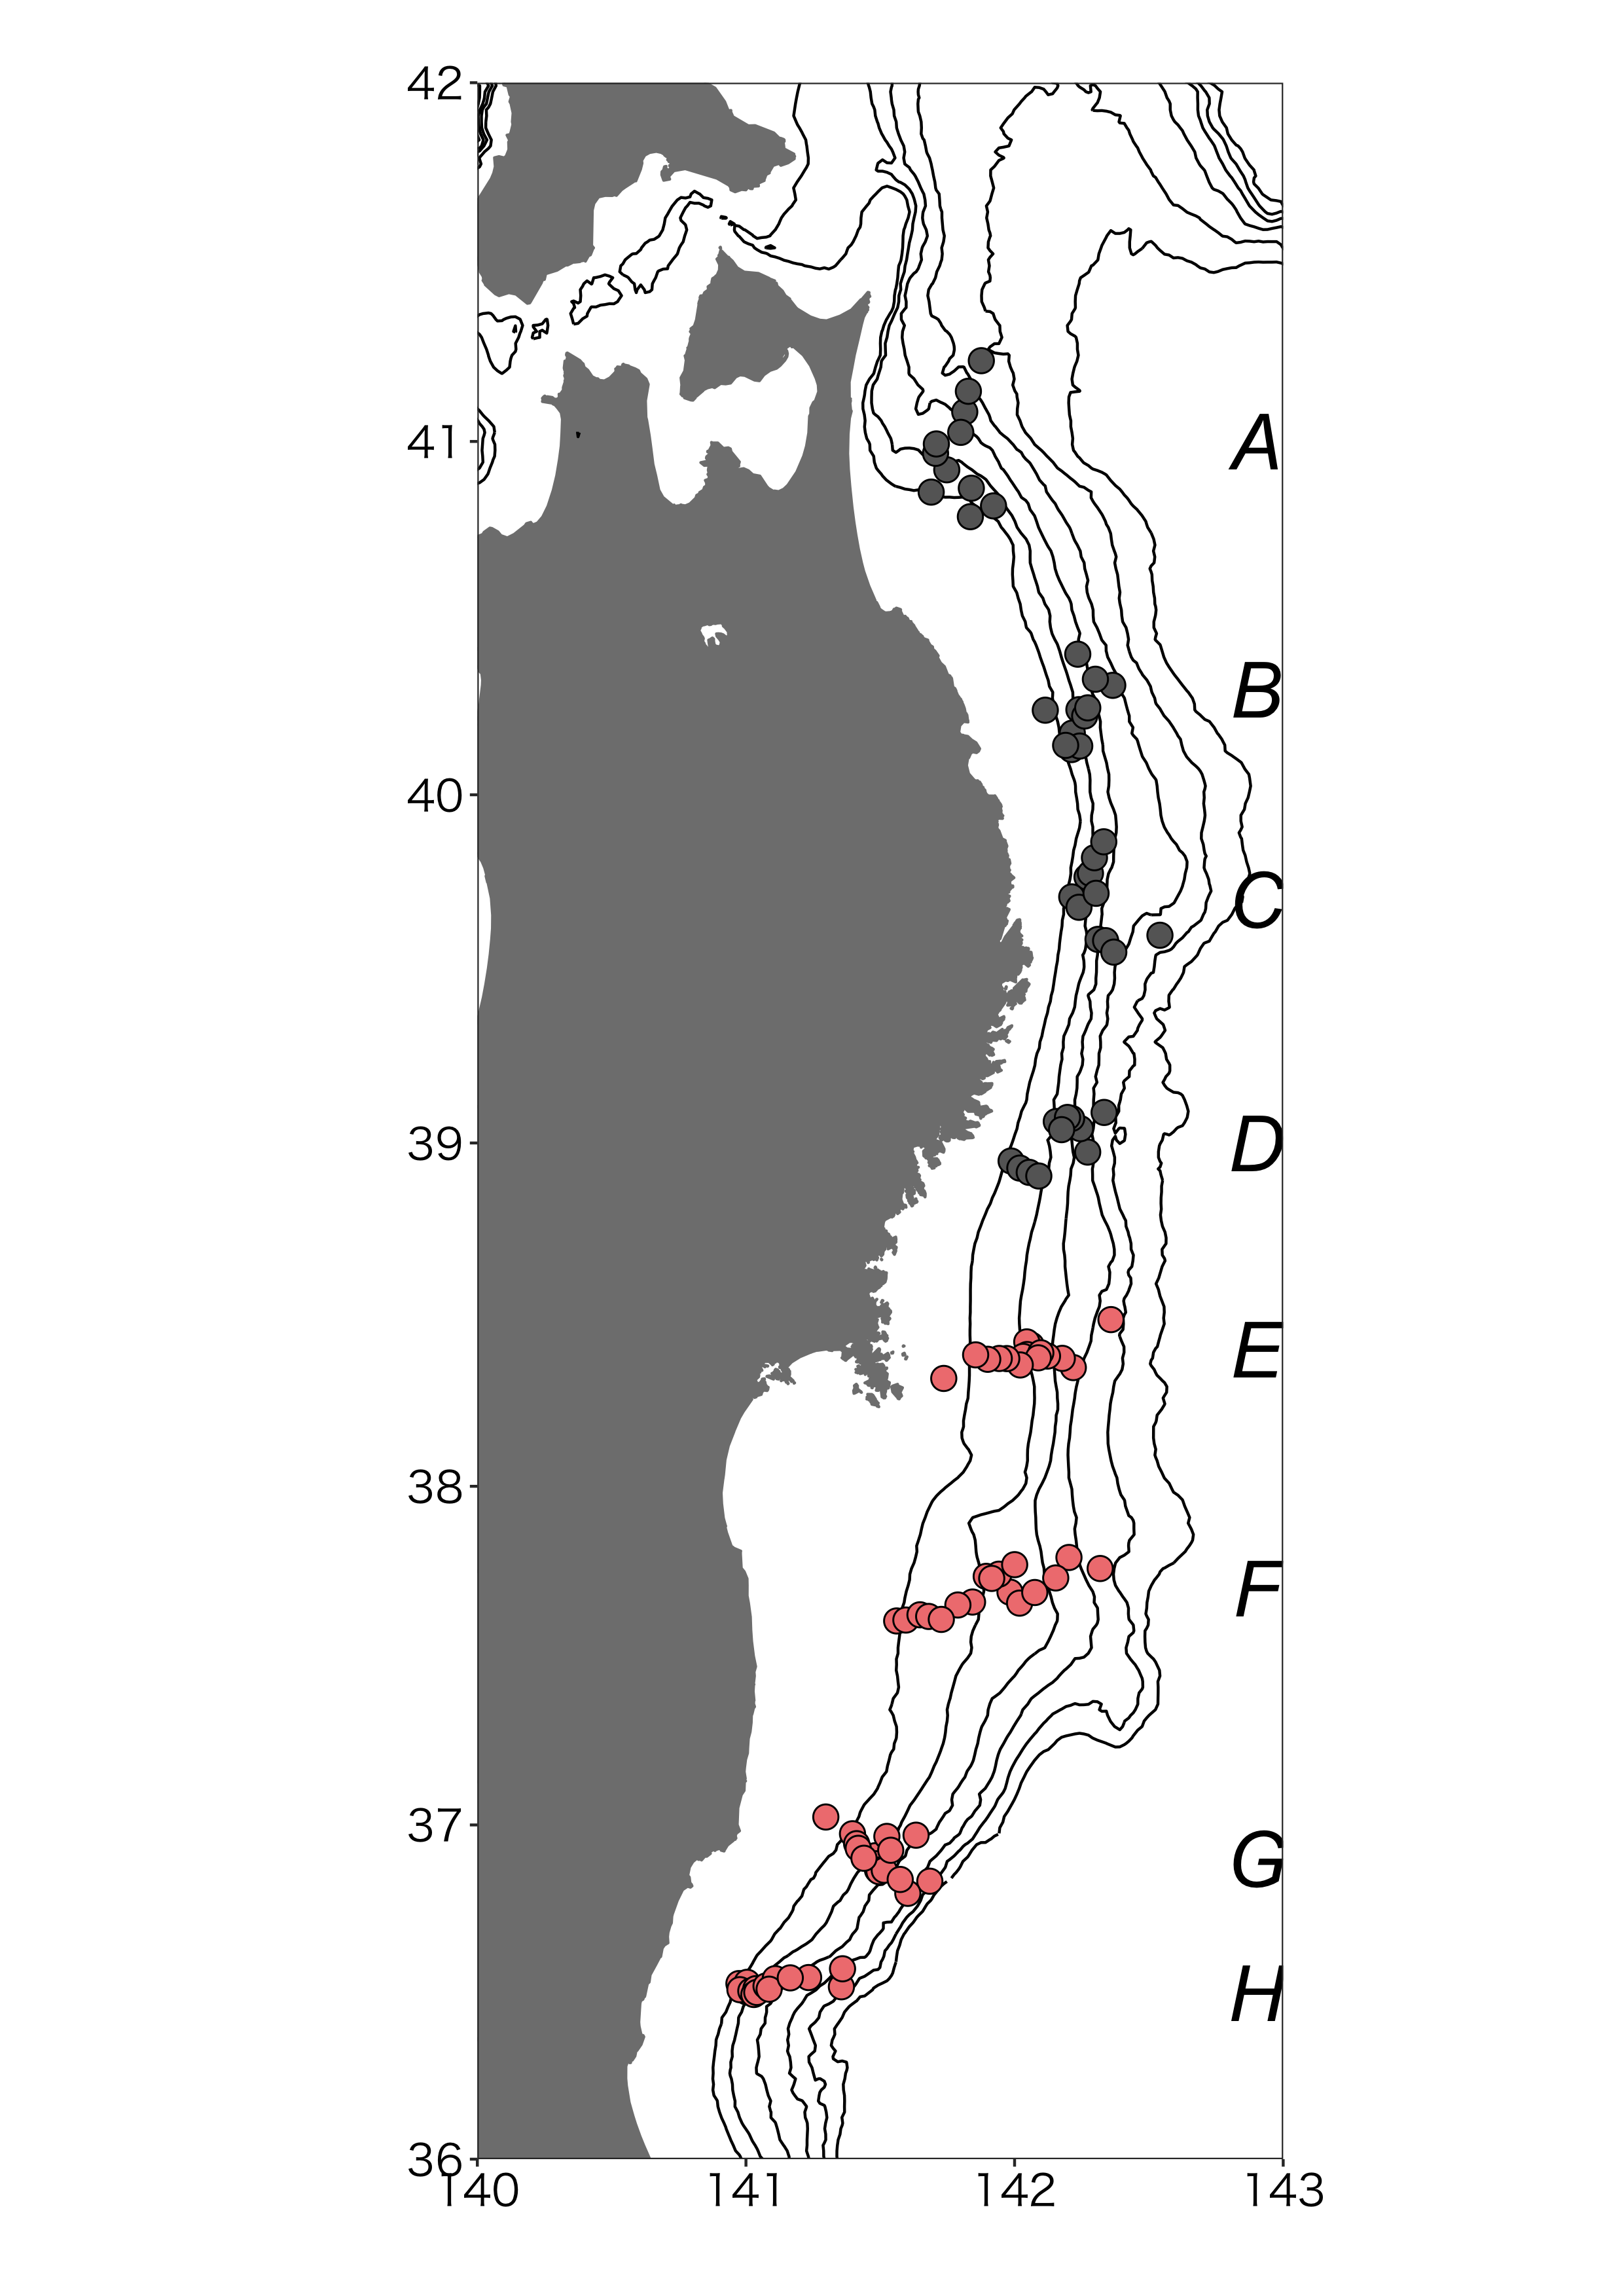
\includegraphics[width = 6cm]{fig1.png}
  \caption{若鷹丸による調査点.黒丸は北部海域,赤丸は南部海域を表す}
\end{figure}

\begin{figure}[h]
  \centering
  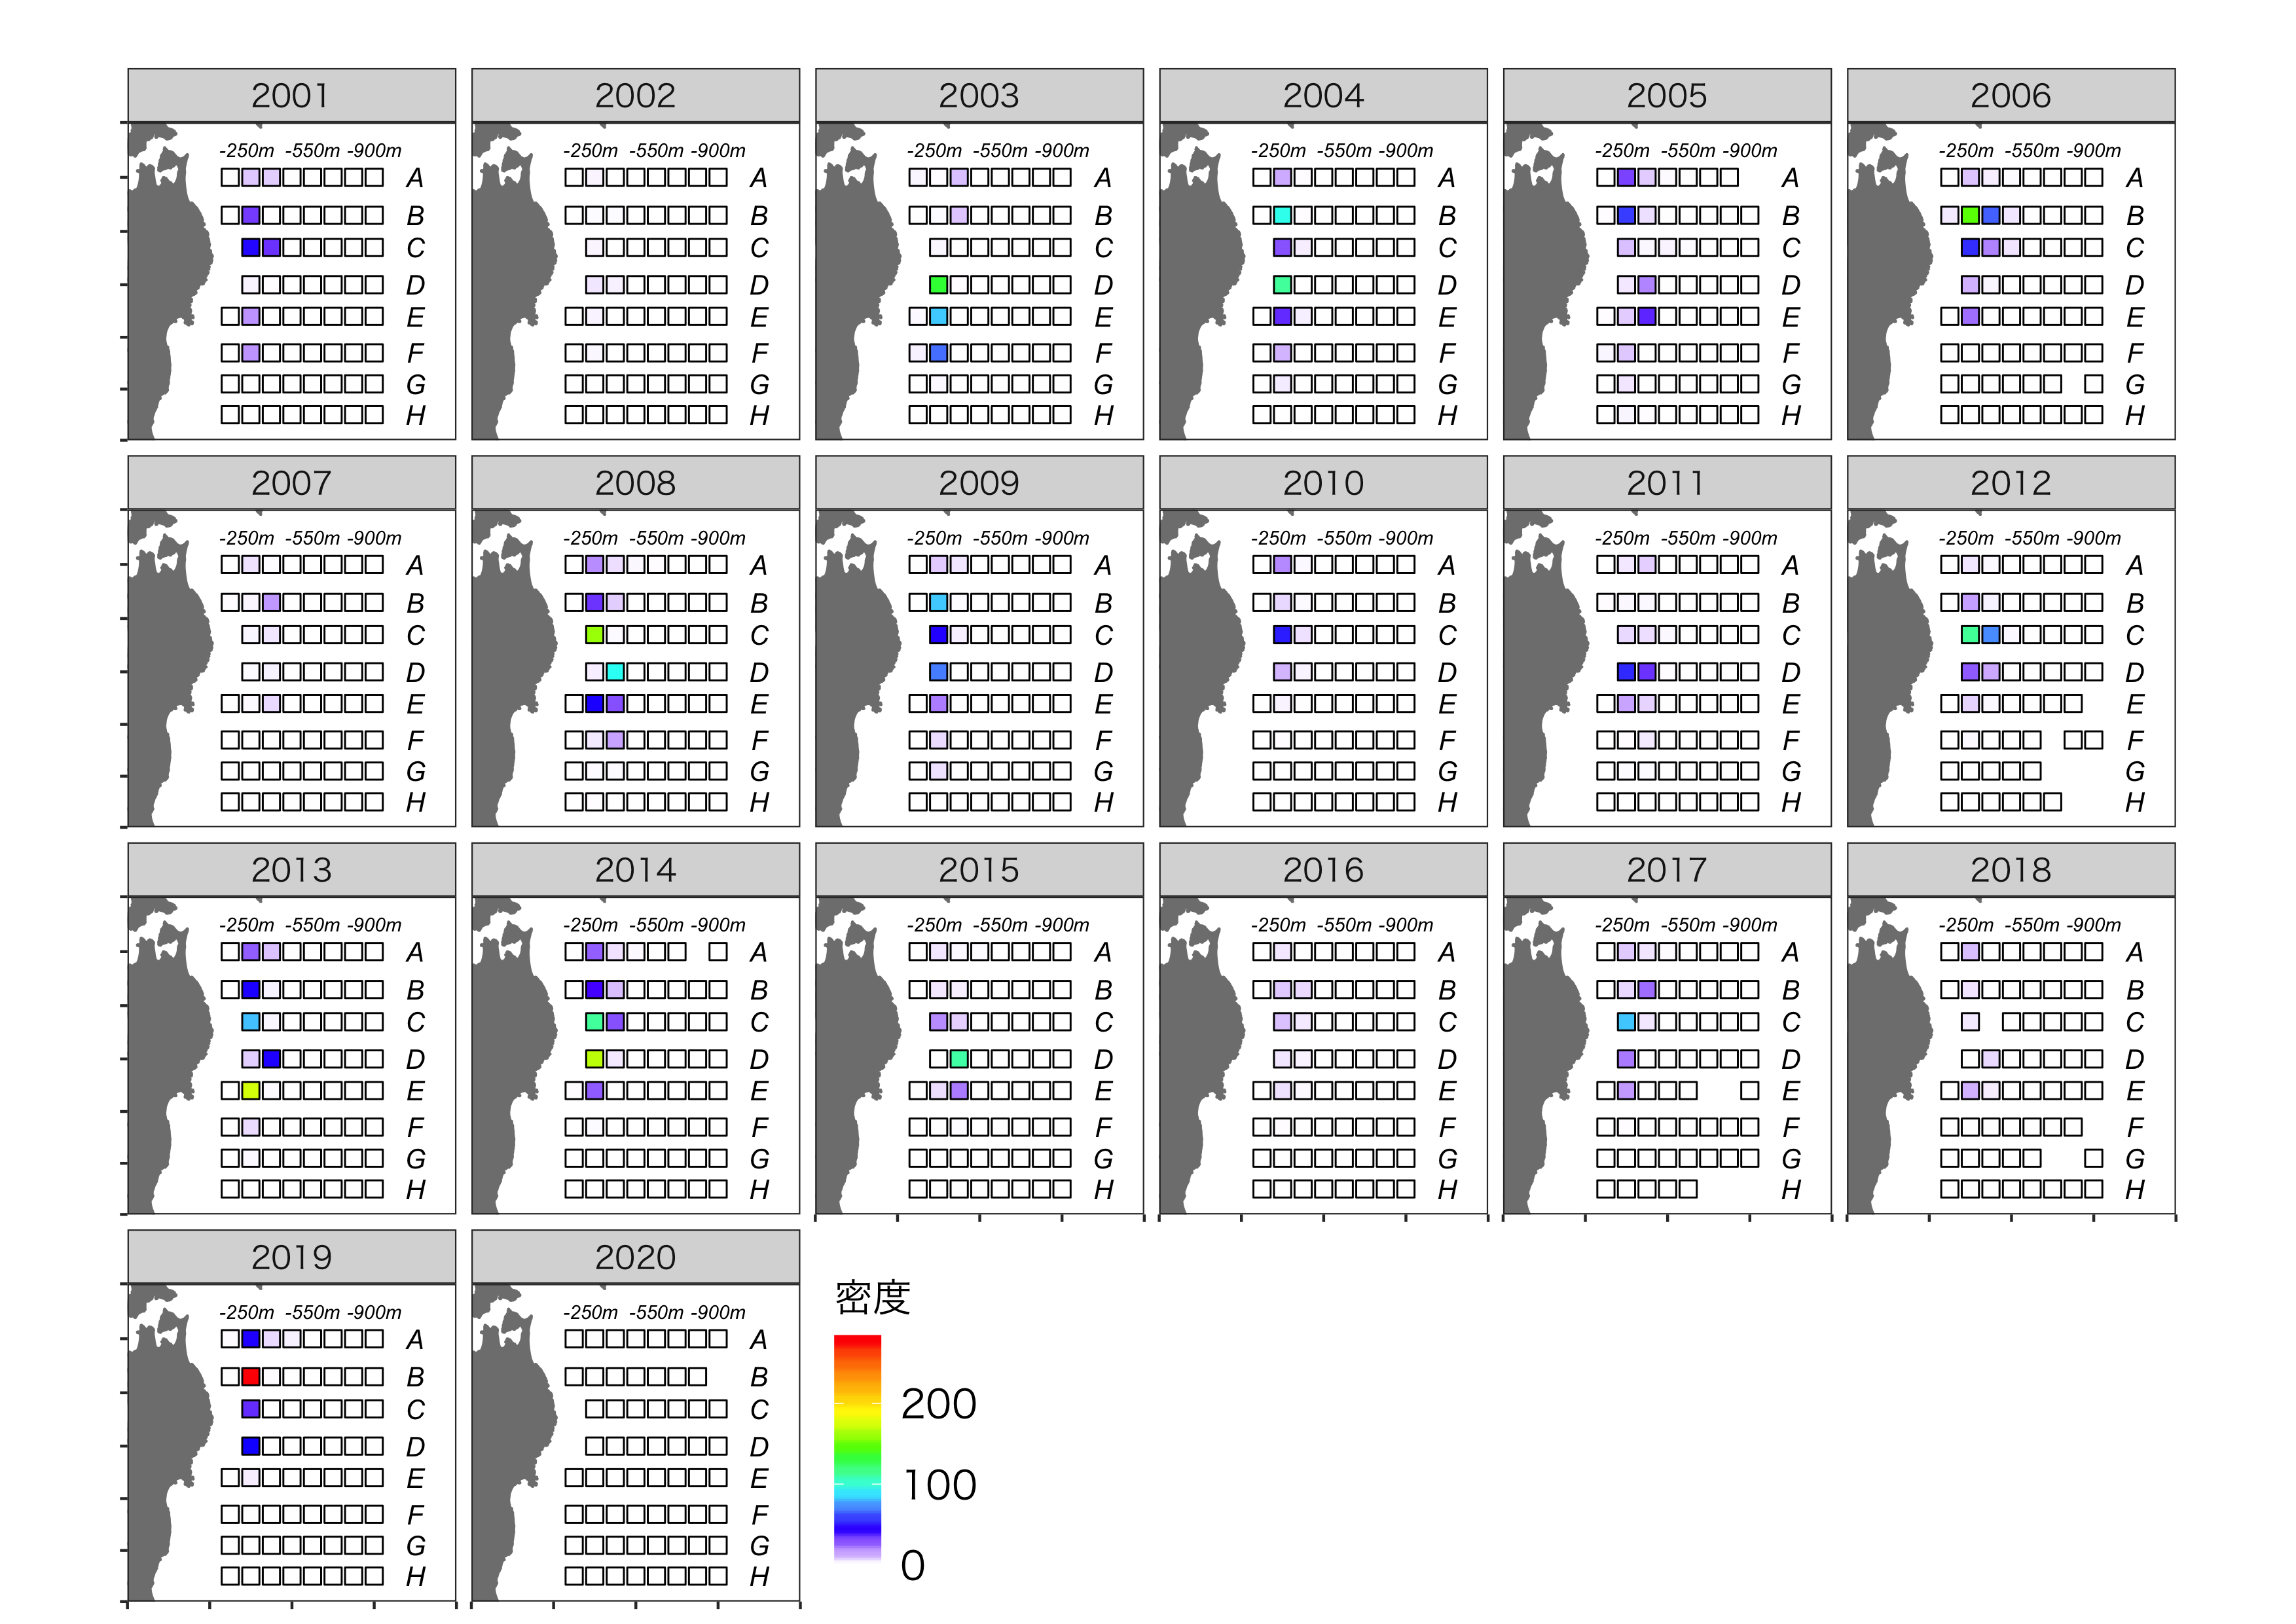
\includegraphics[width = 14cm]{スケトウダラ0+dens.png}
  \caption{スケトウダラ0歳魚の分布密度(千尾/km2)の経年変化}
\end{figure}

\begin{figure}[h]
  \centering
  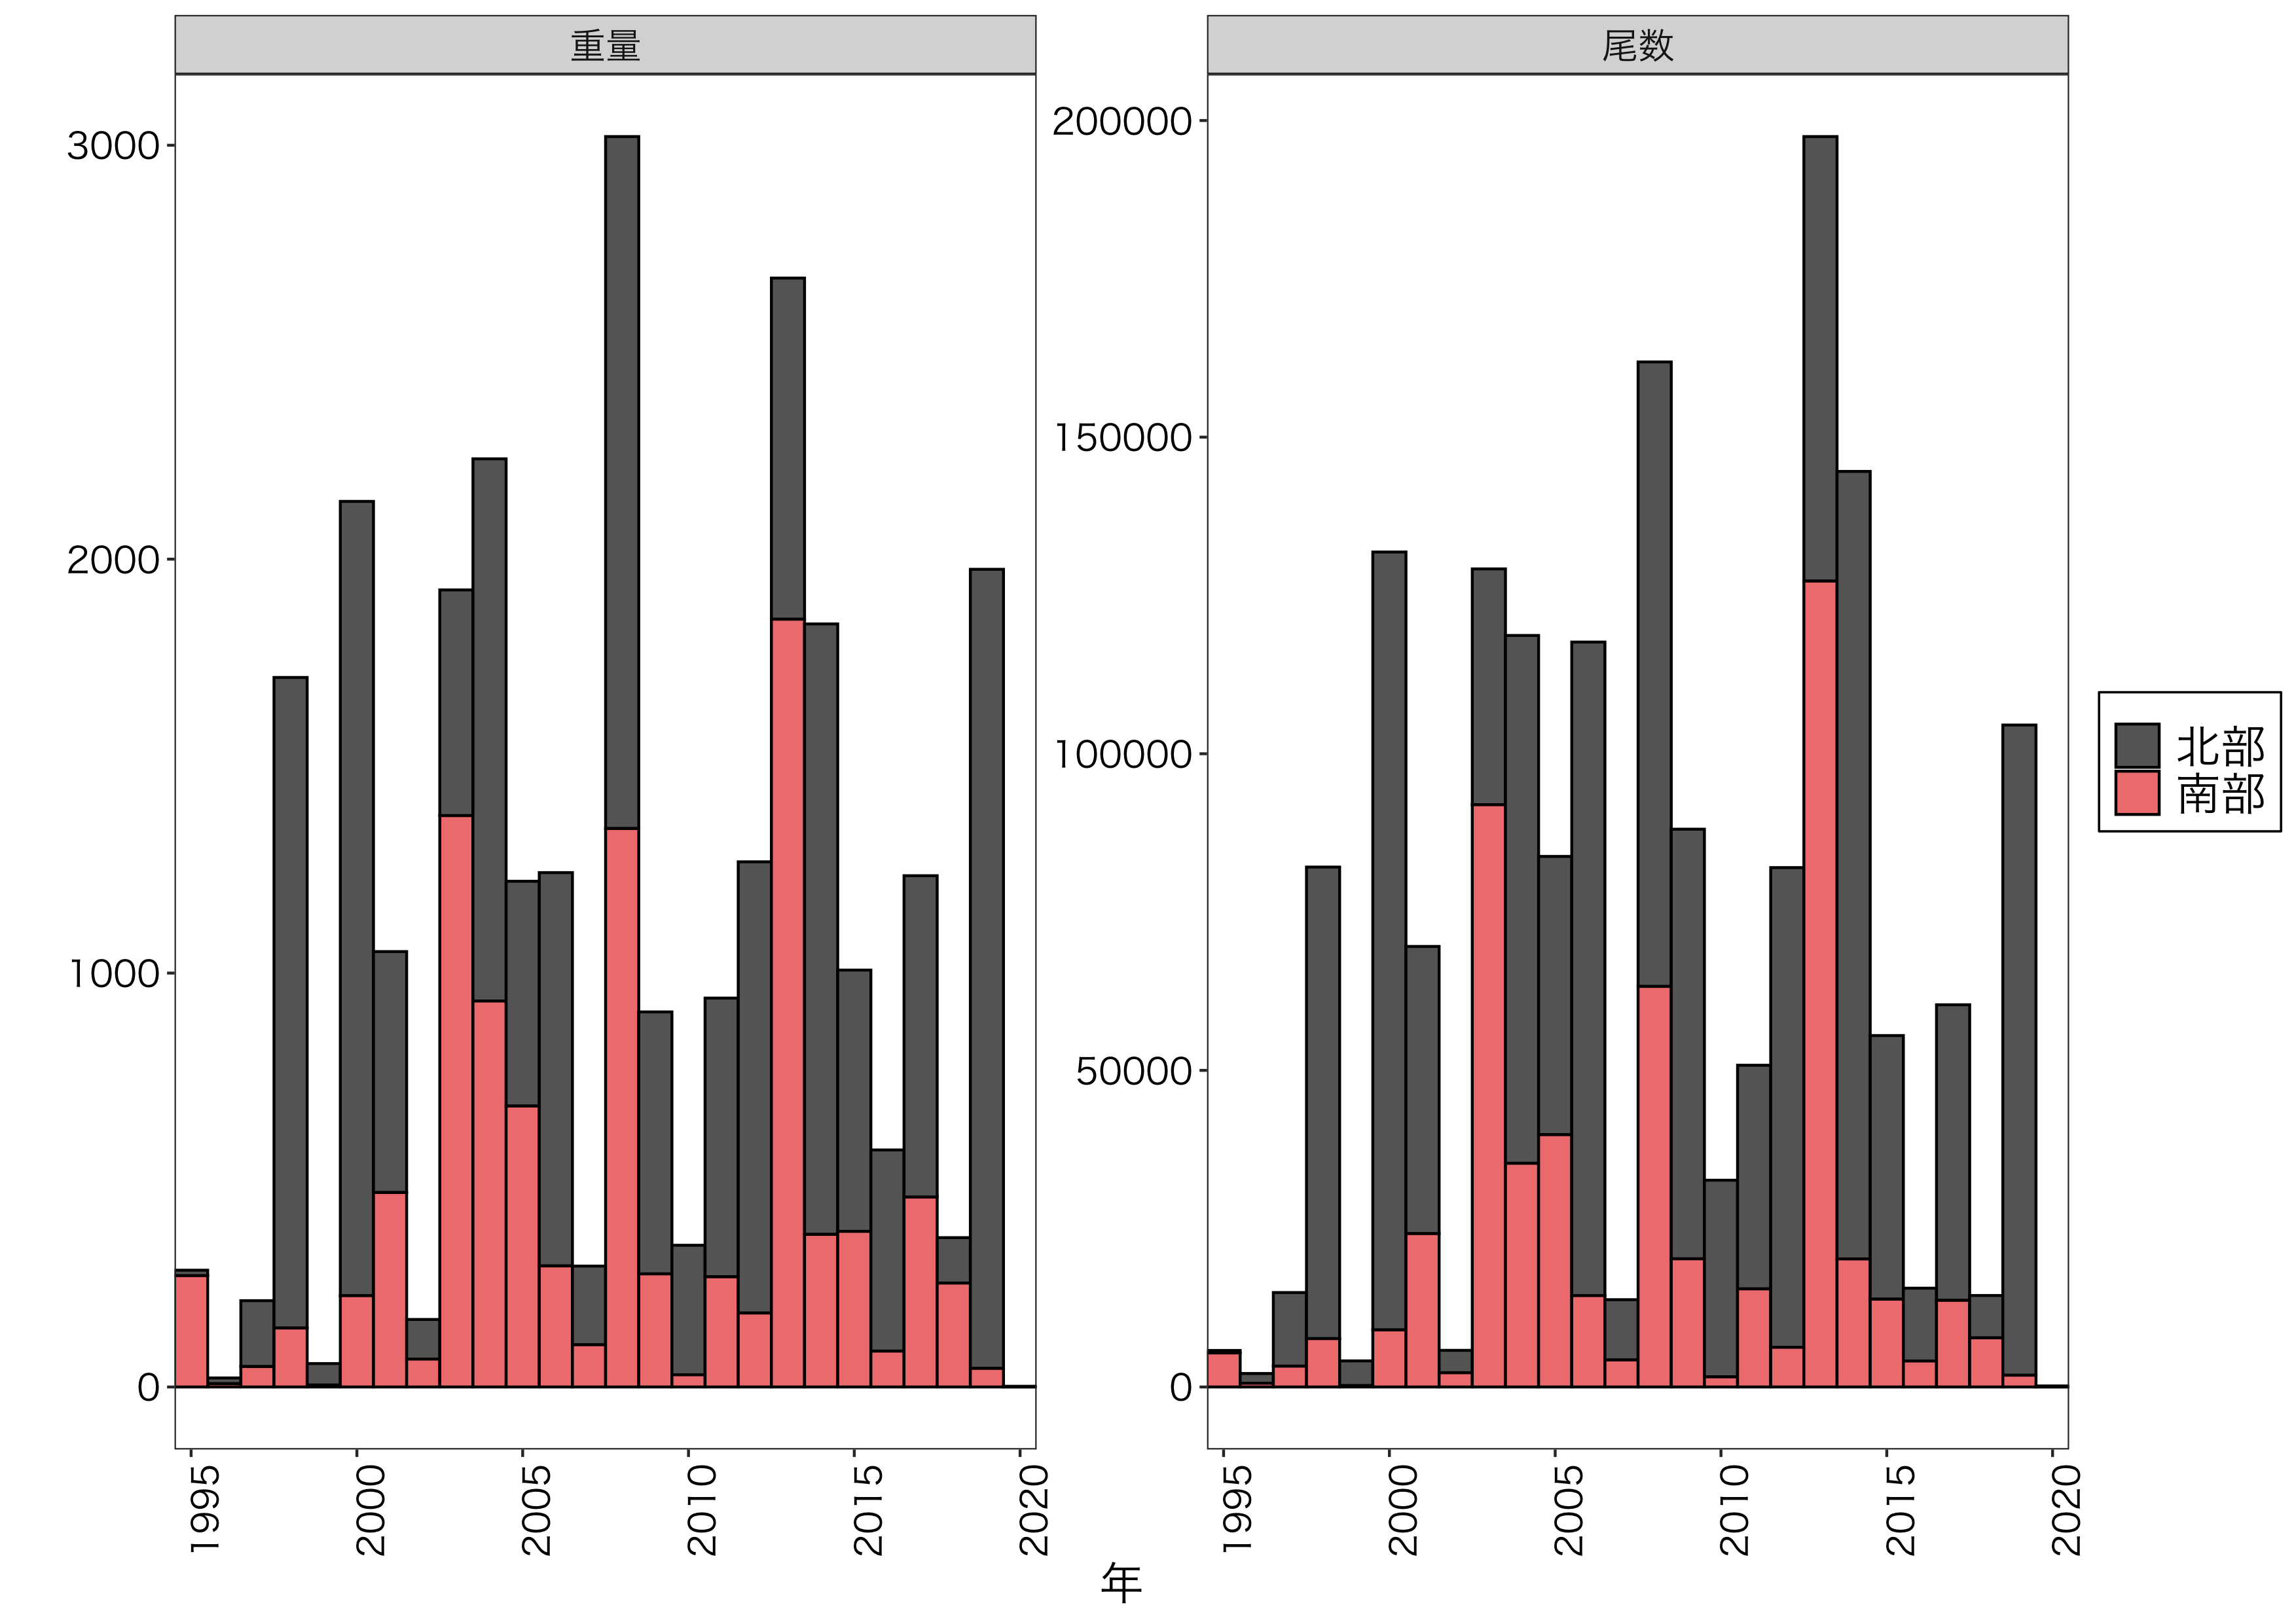
\includegraphics[width = 14cm]{スケトウダラ0+trend.png}
  \caption{スケトウダラ0歳魚の現存量(右; 単位は千トン)と現存尾数(左; 単位は百万尾)の経年変化}
\end{figure}

\begin{figure}[h]
  \centering
  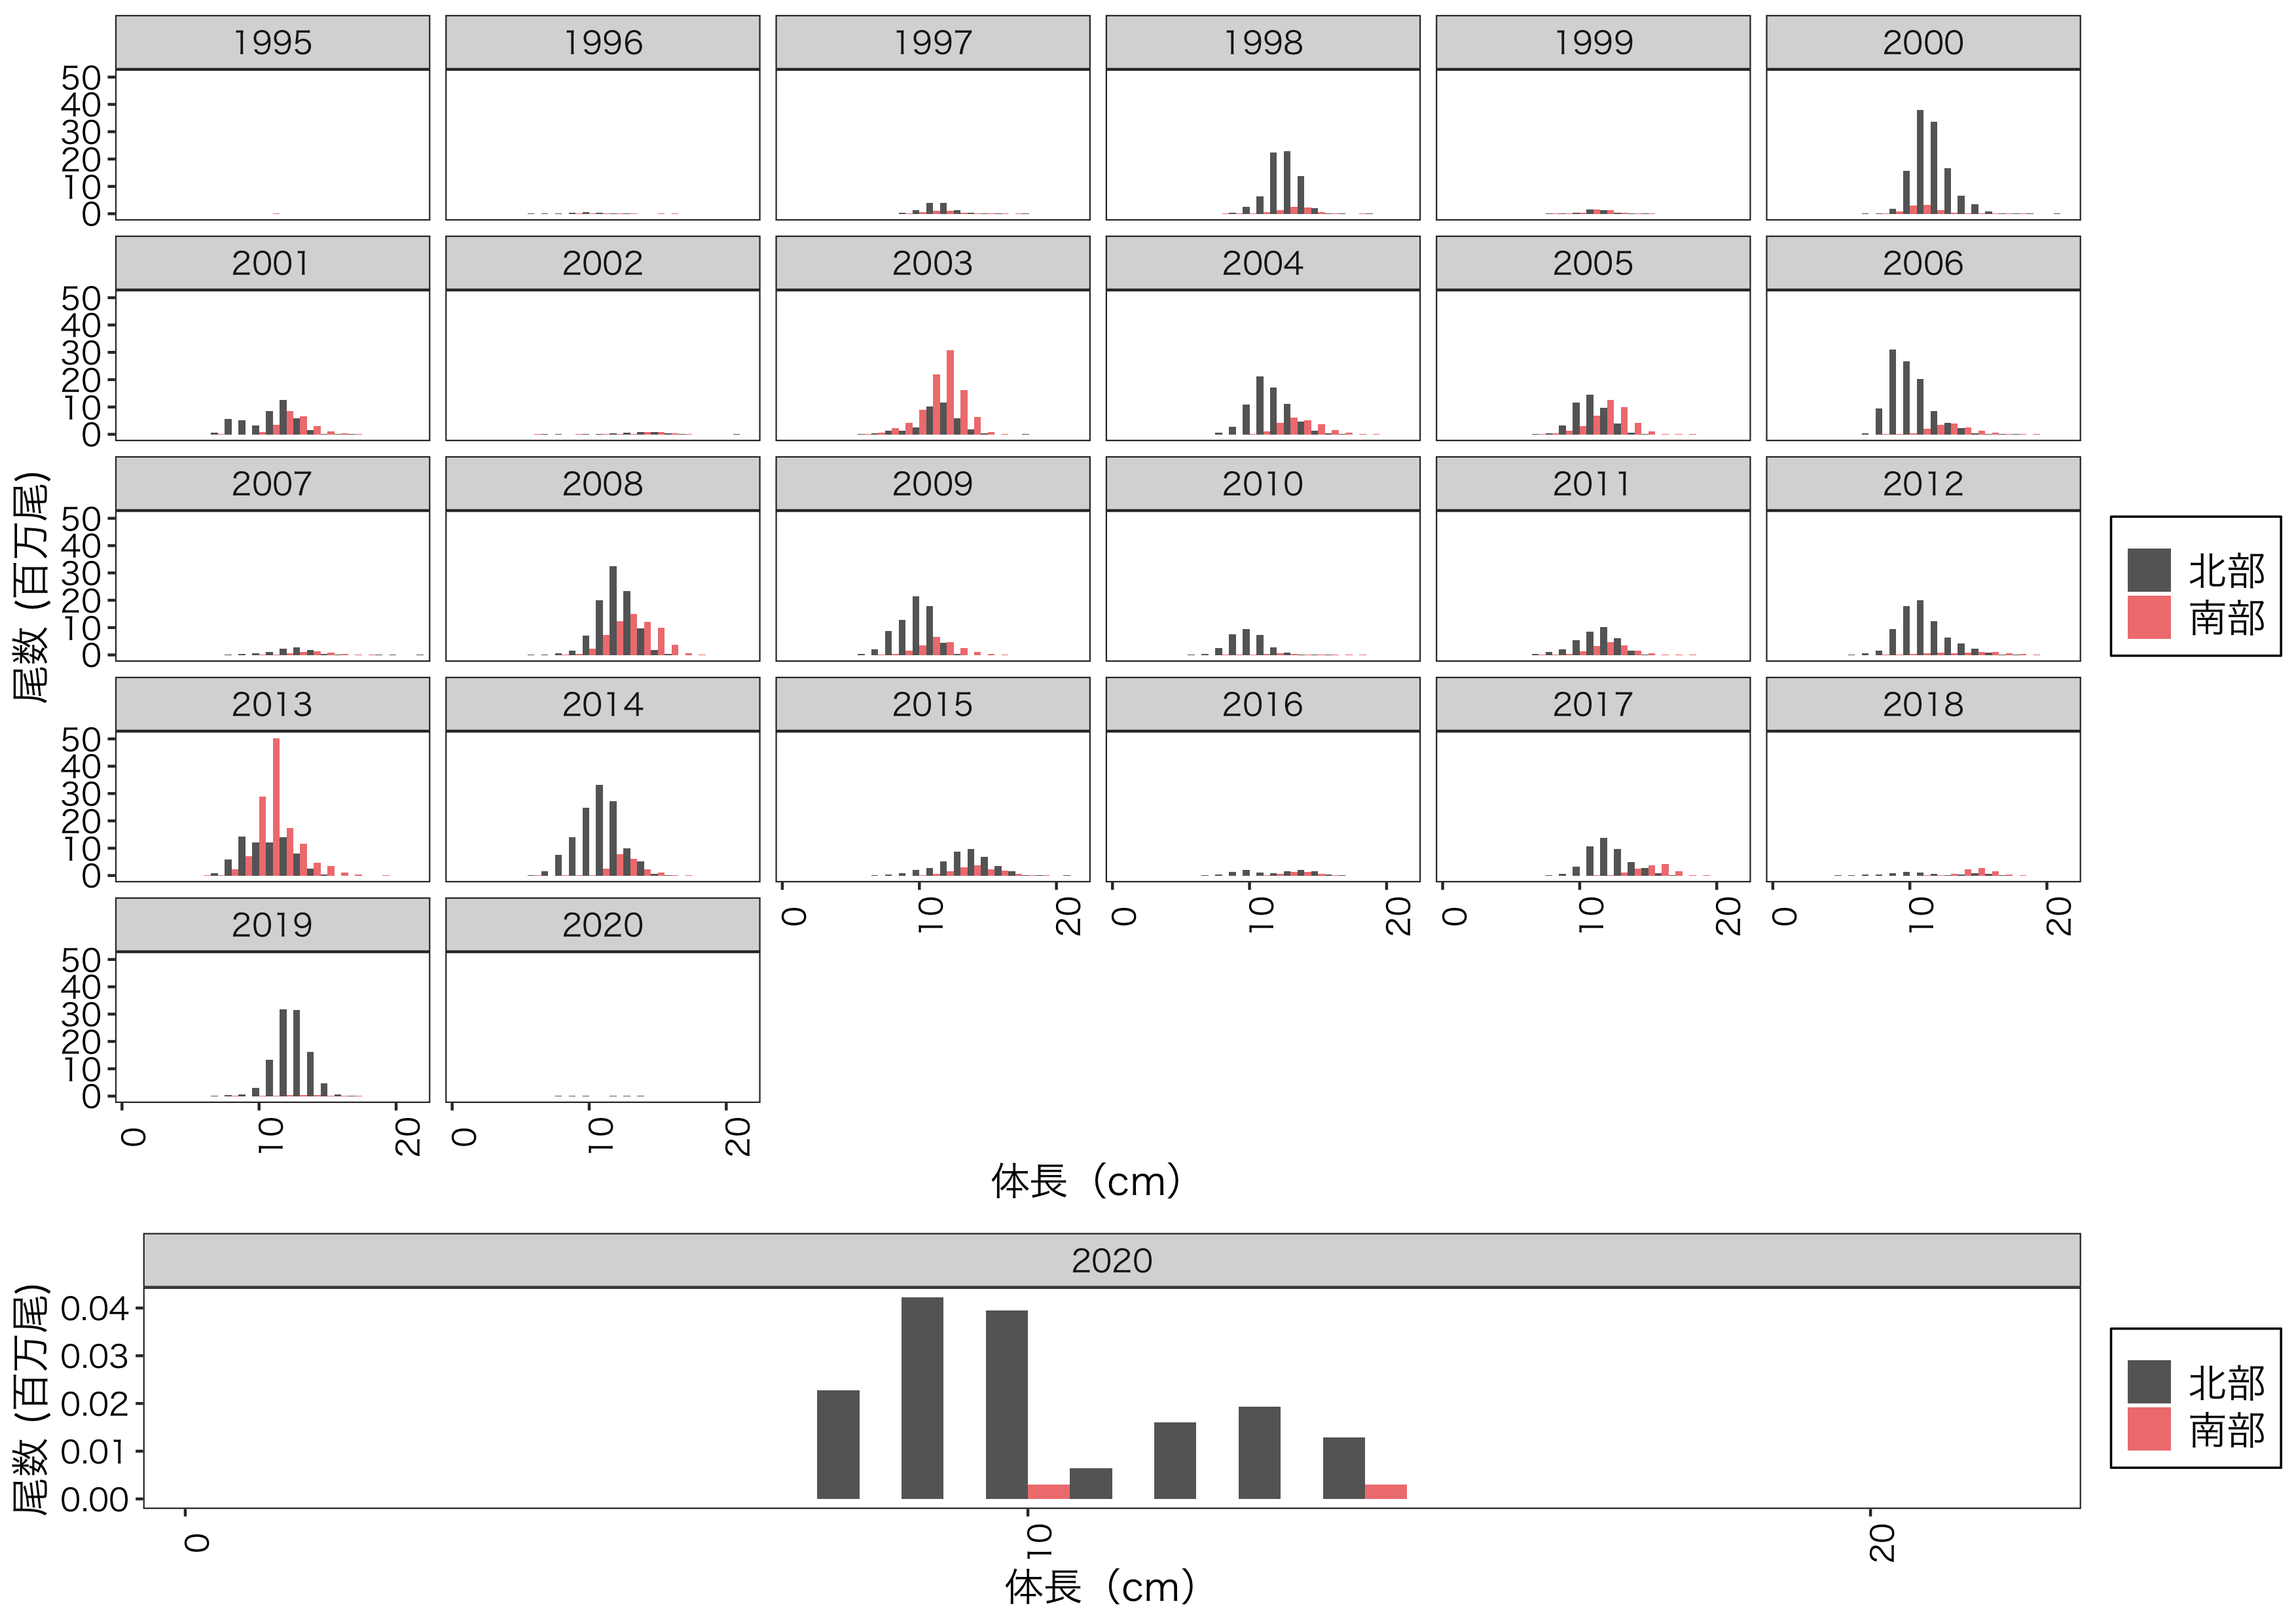
\includegraphics[width = 14cm]{スケトウダラ0+length.png}
  \caption{スケトウダラ0歳魚の体長組成の経年変化}
\end{figure}

\begin{figure}[h]
  \centering
  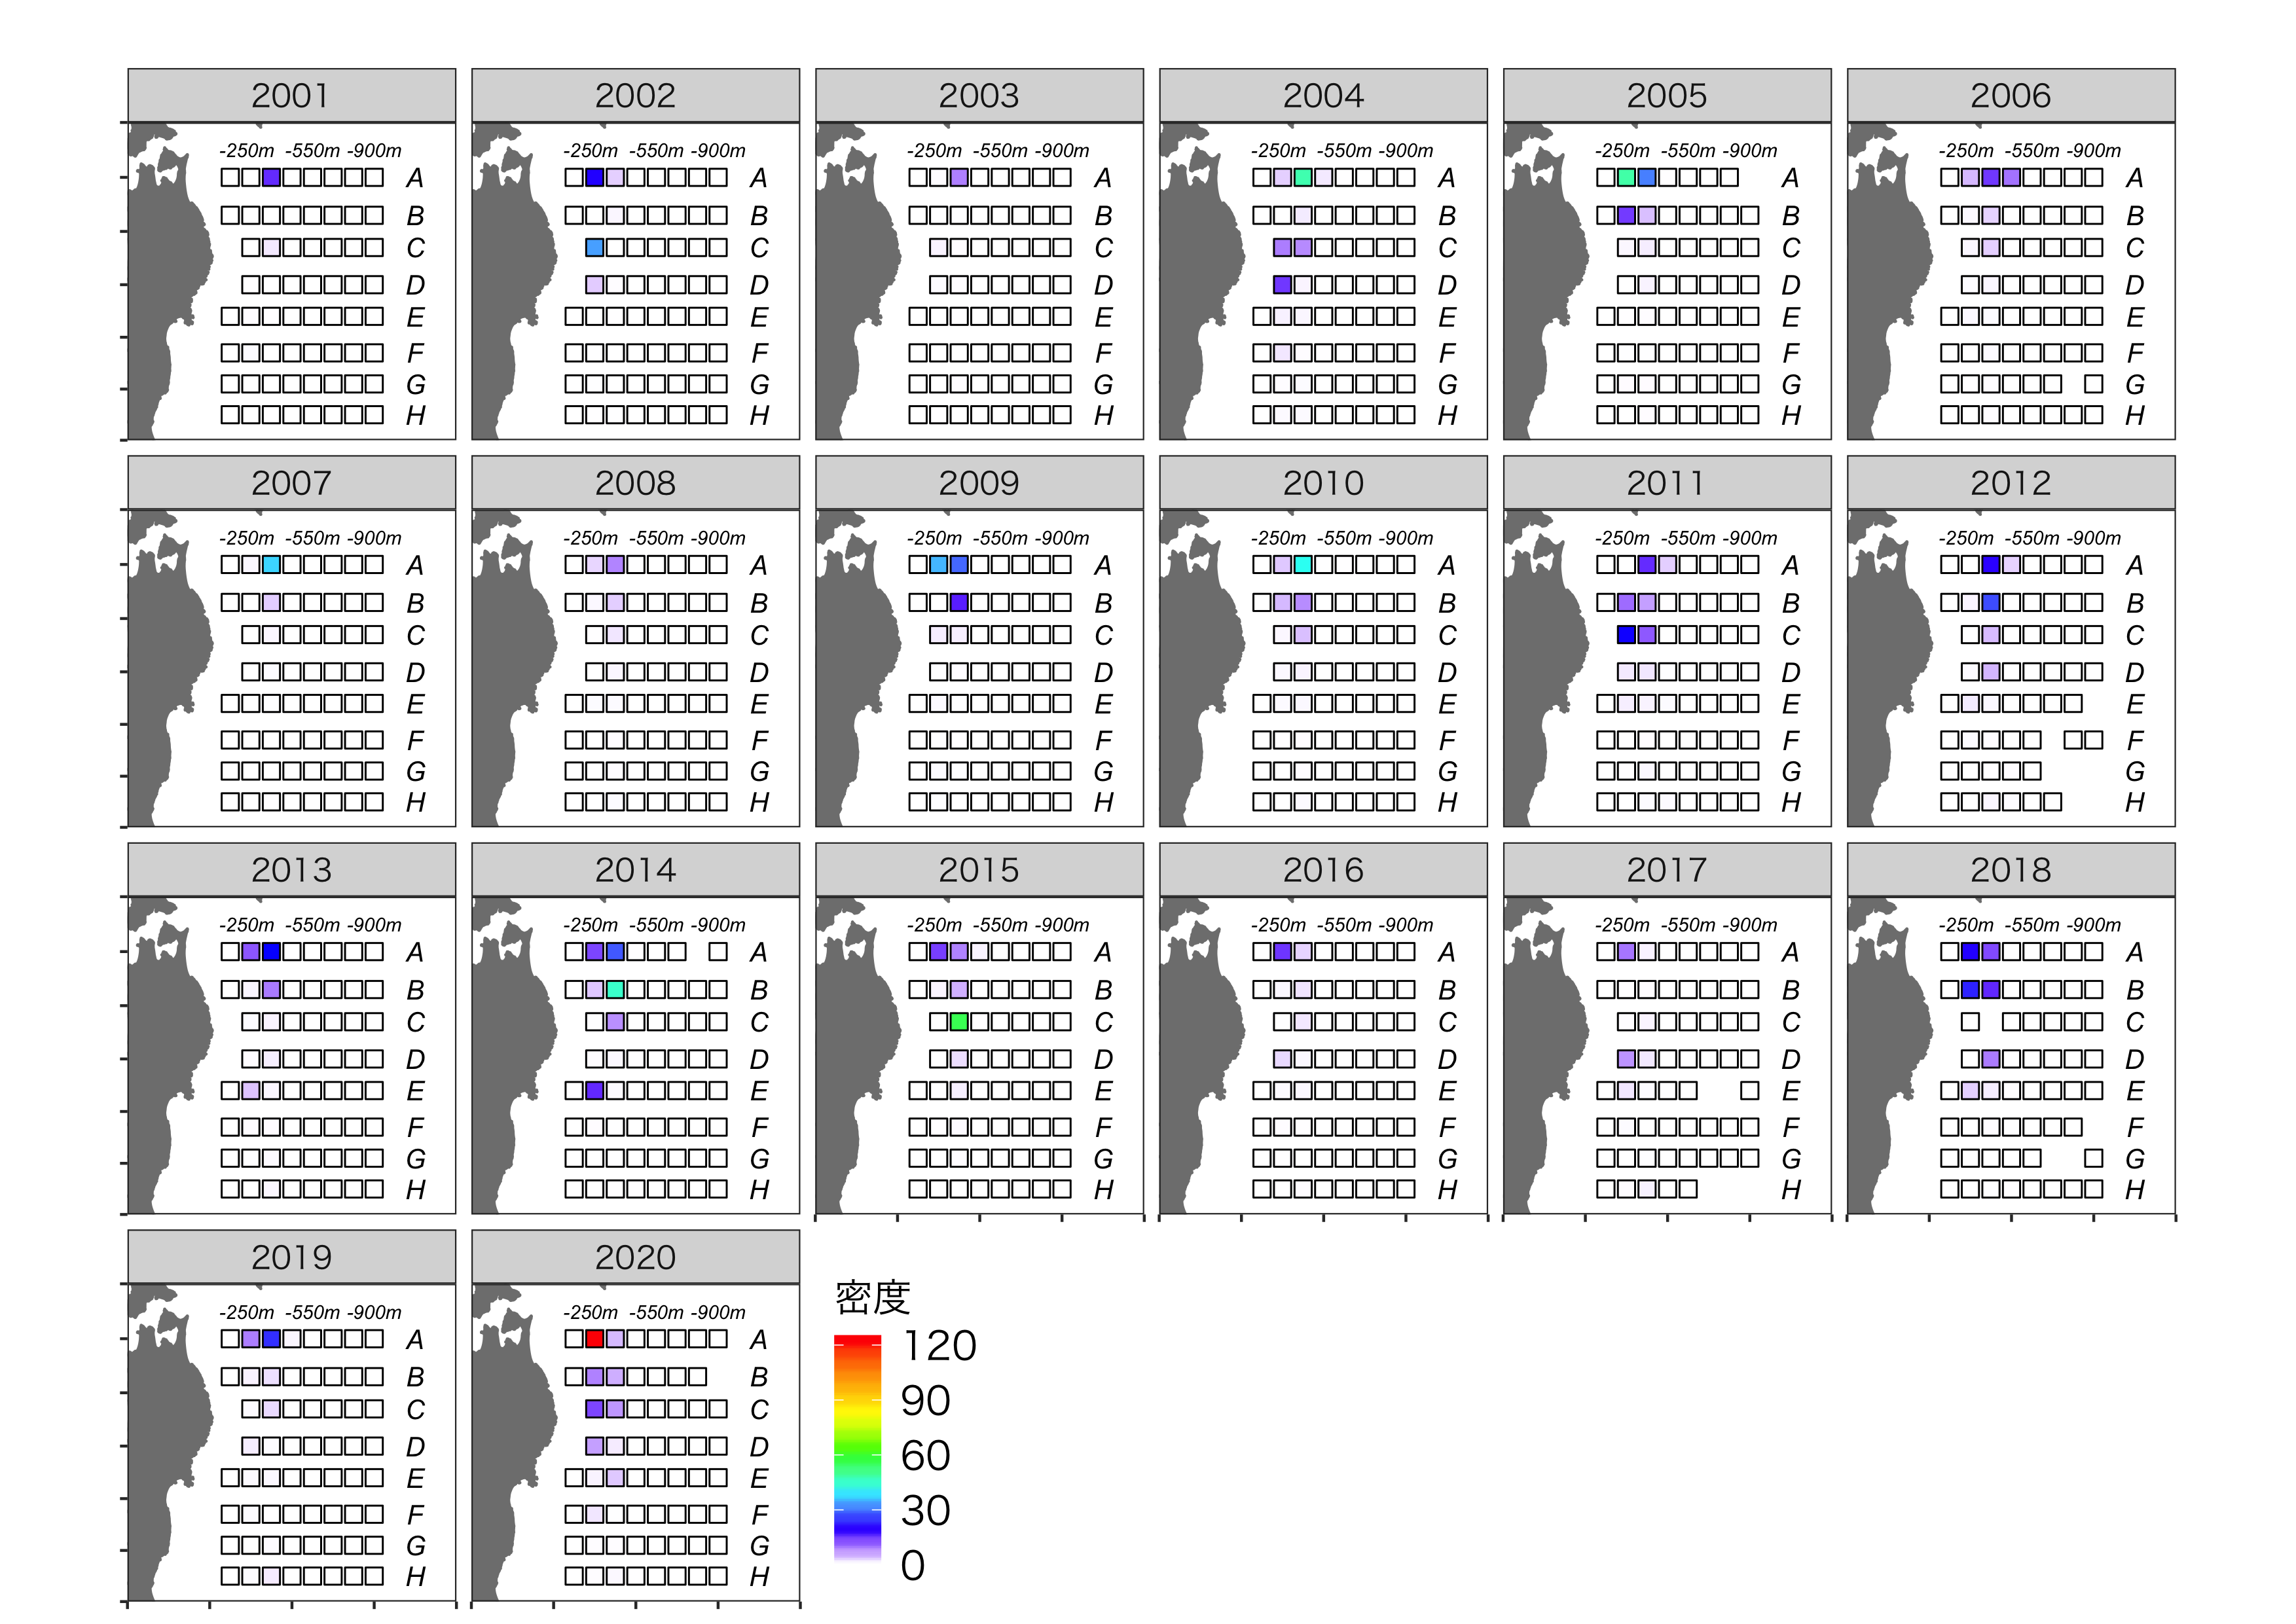
\includegraphics[width = 14cm]{スケトウダラ1+dens.png}
  \caption{スケトウダラ1歳魚以上の分布密度(千尾/km2)の経年変化}
\end{figure}

\begin{figure}[h]
  \centering
  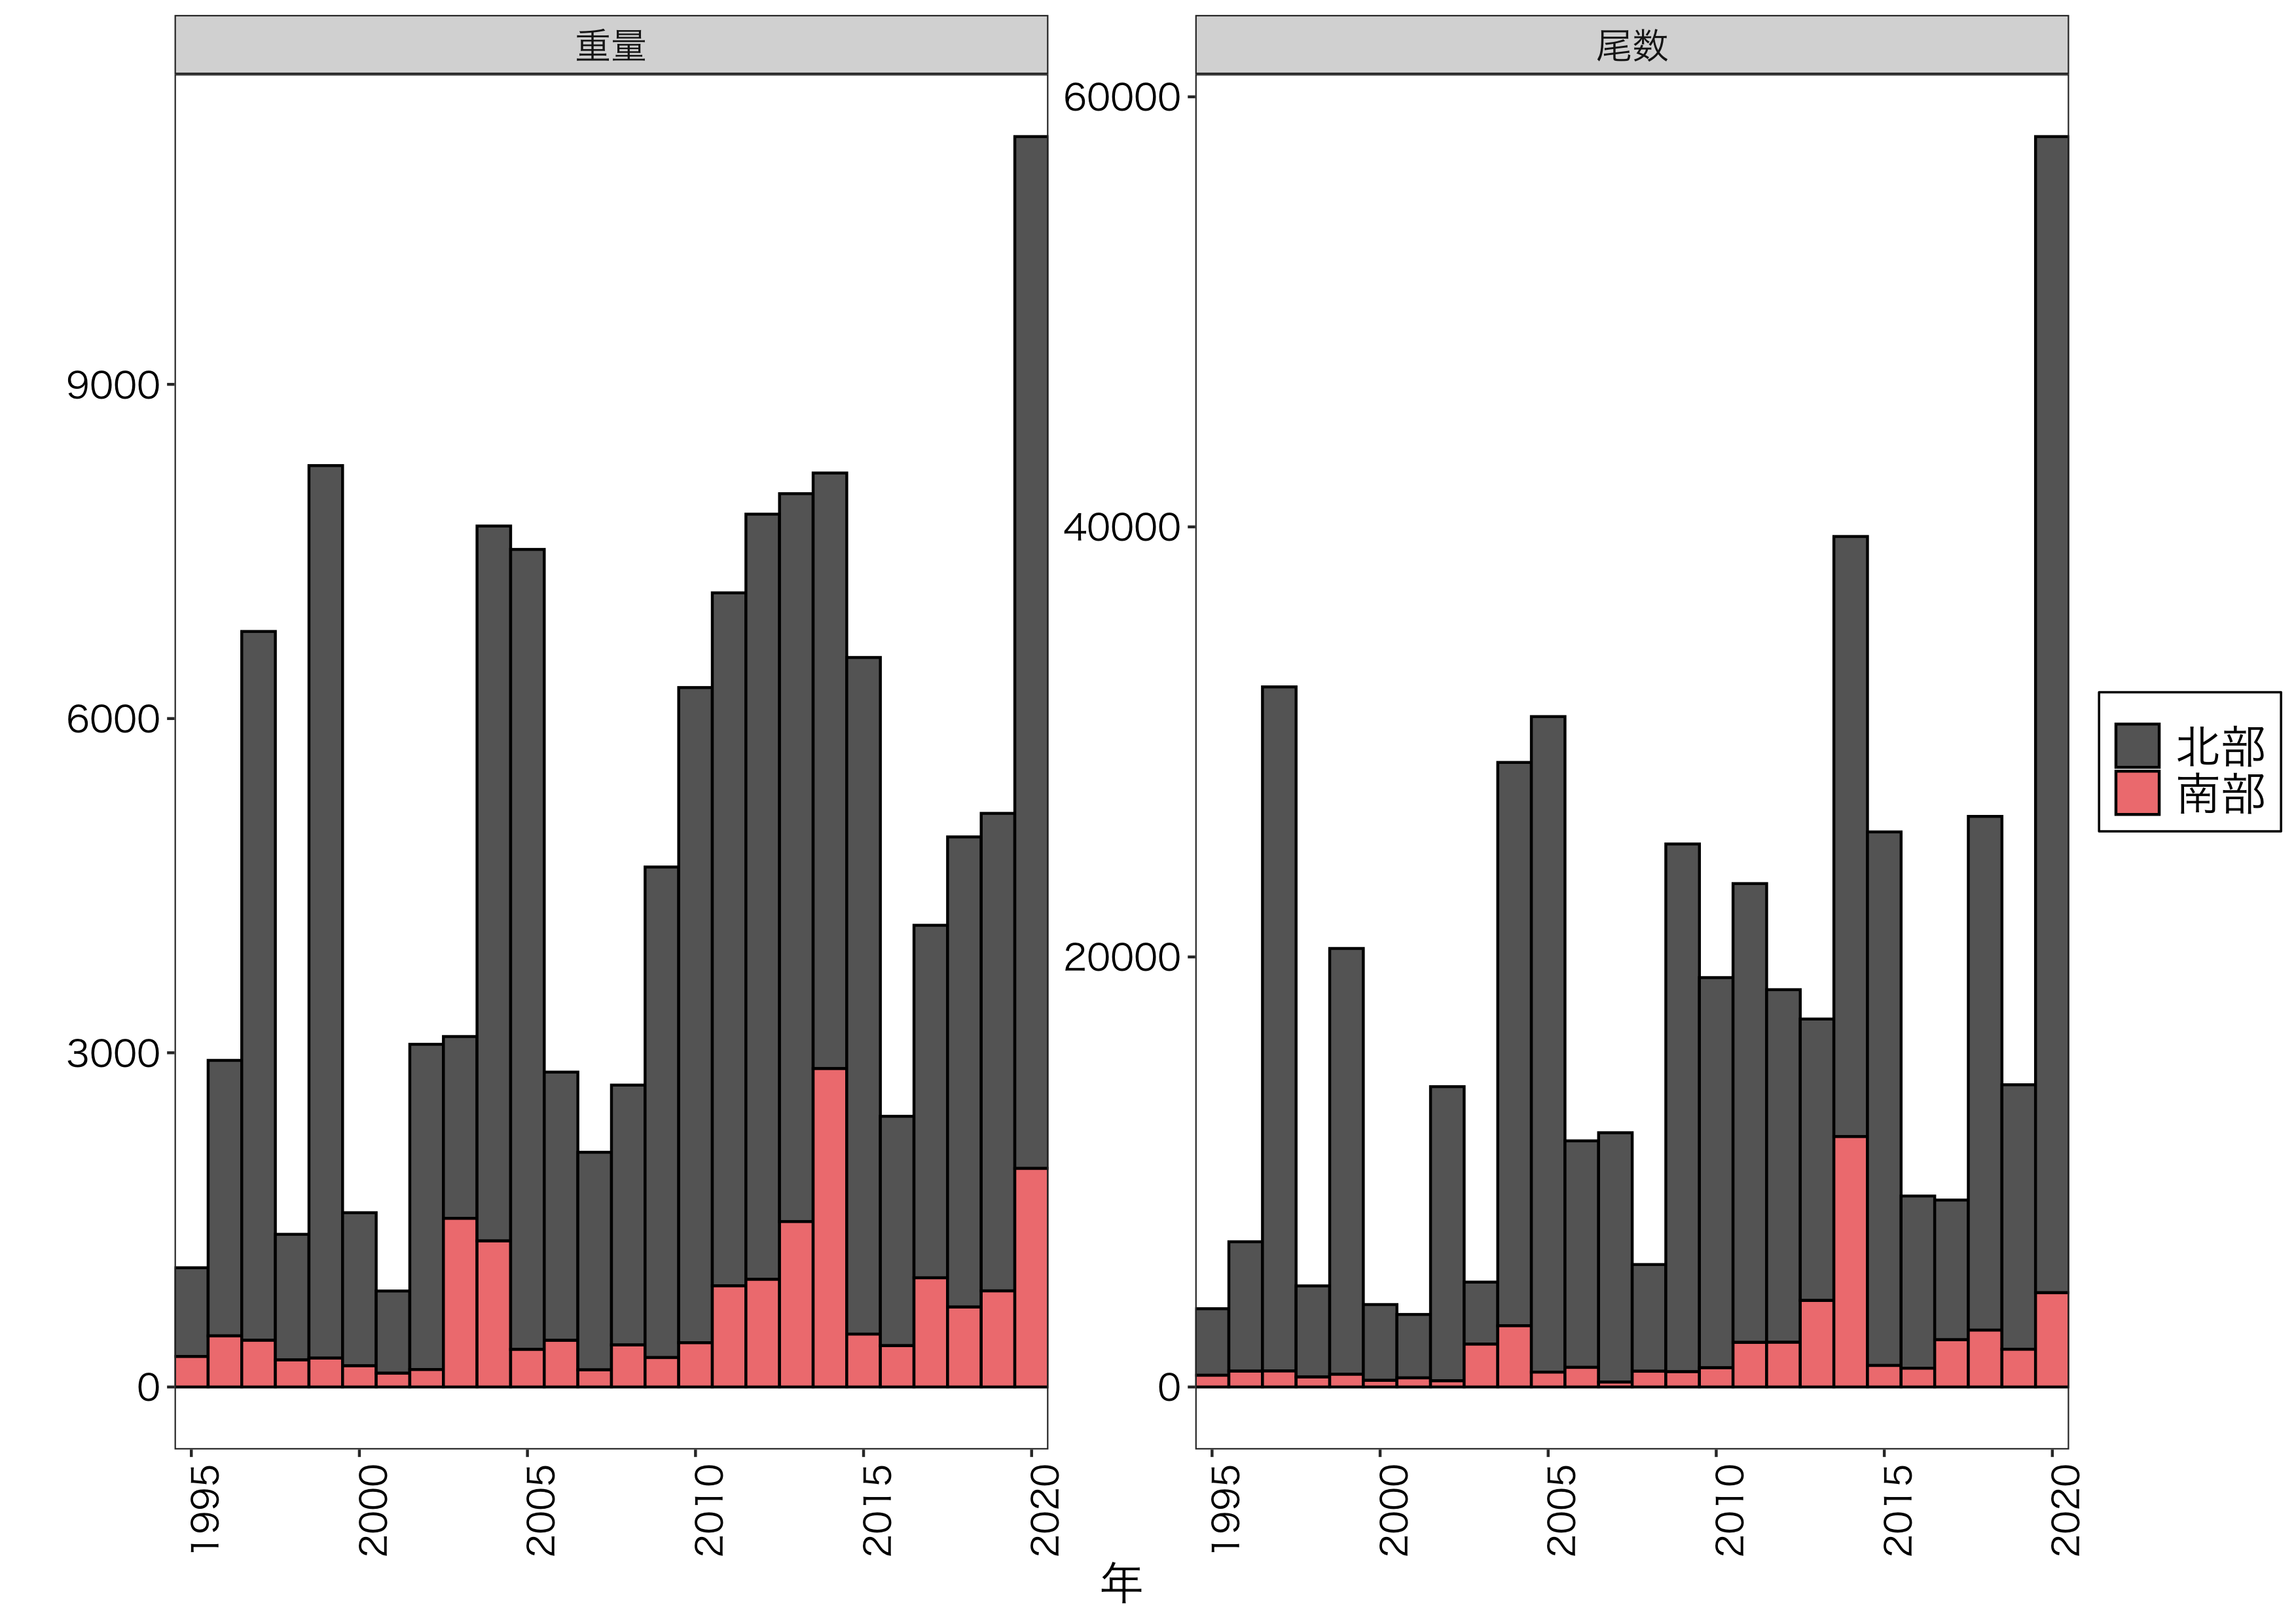
\includegraphics[width = 14cm]{スケトウダラ1+trend.png}
  \caption{スケトウダラ1歳魚以上の現存量(右; 単位は千トン)と現存尾数(左; 単位は百万尾)の経年変化}
\end{figure}

\begin{figure}[h]
  \centering
  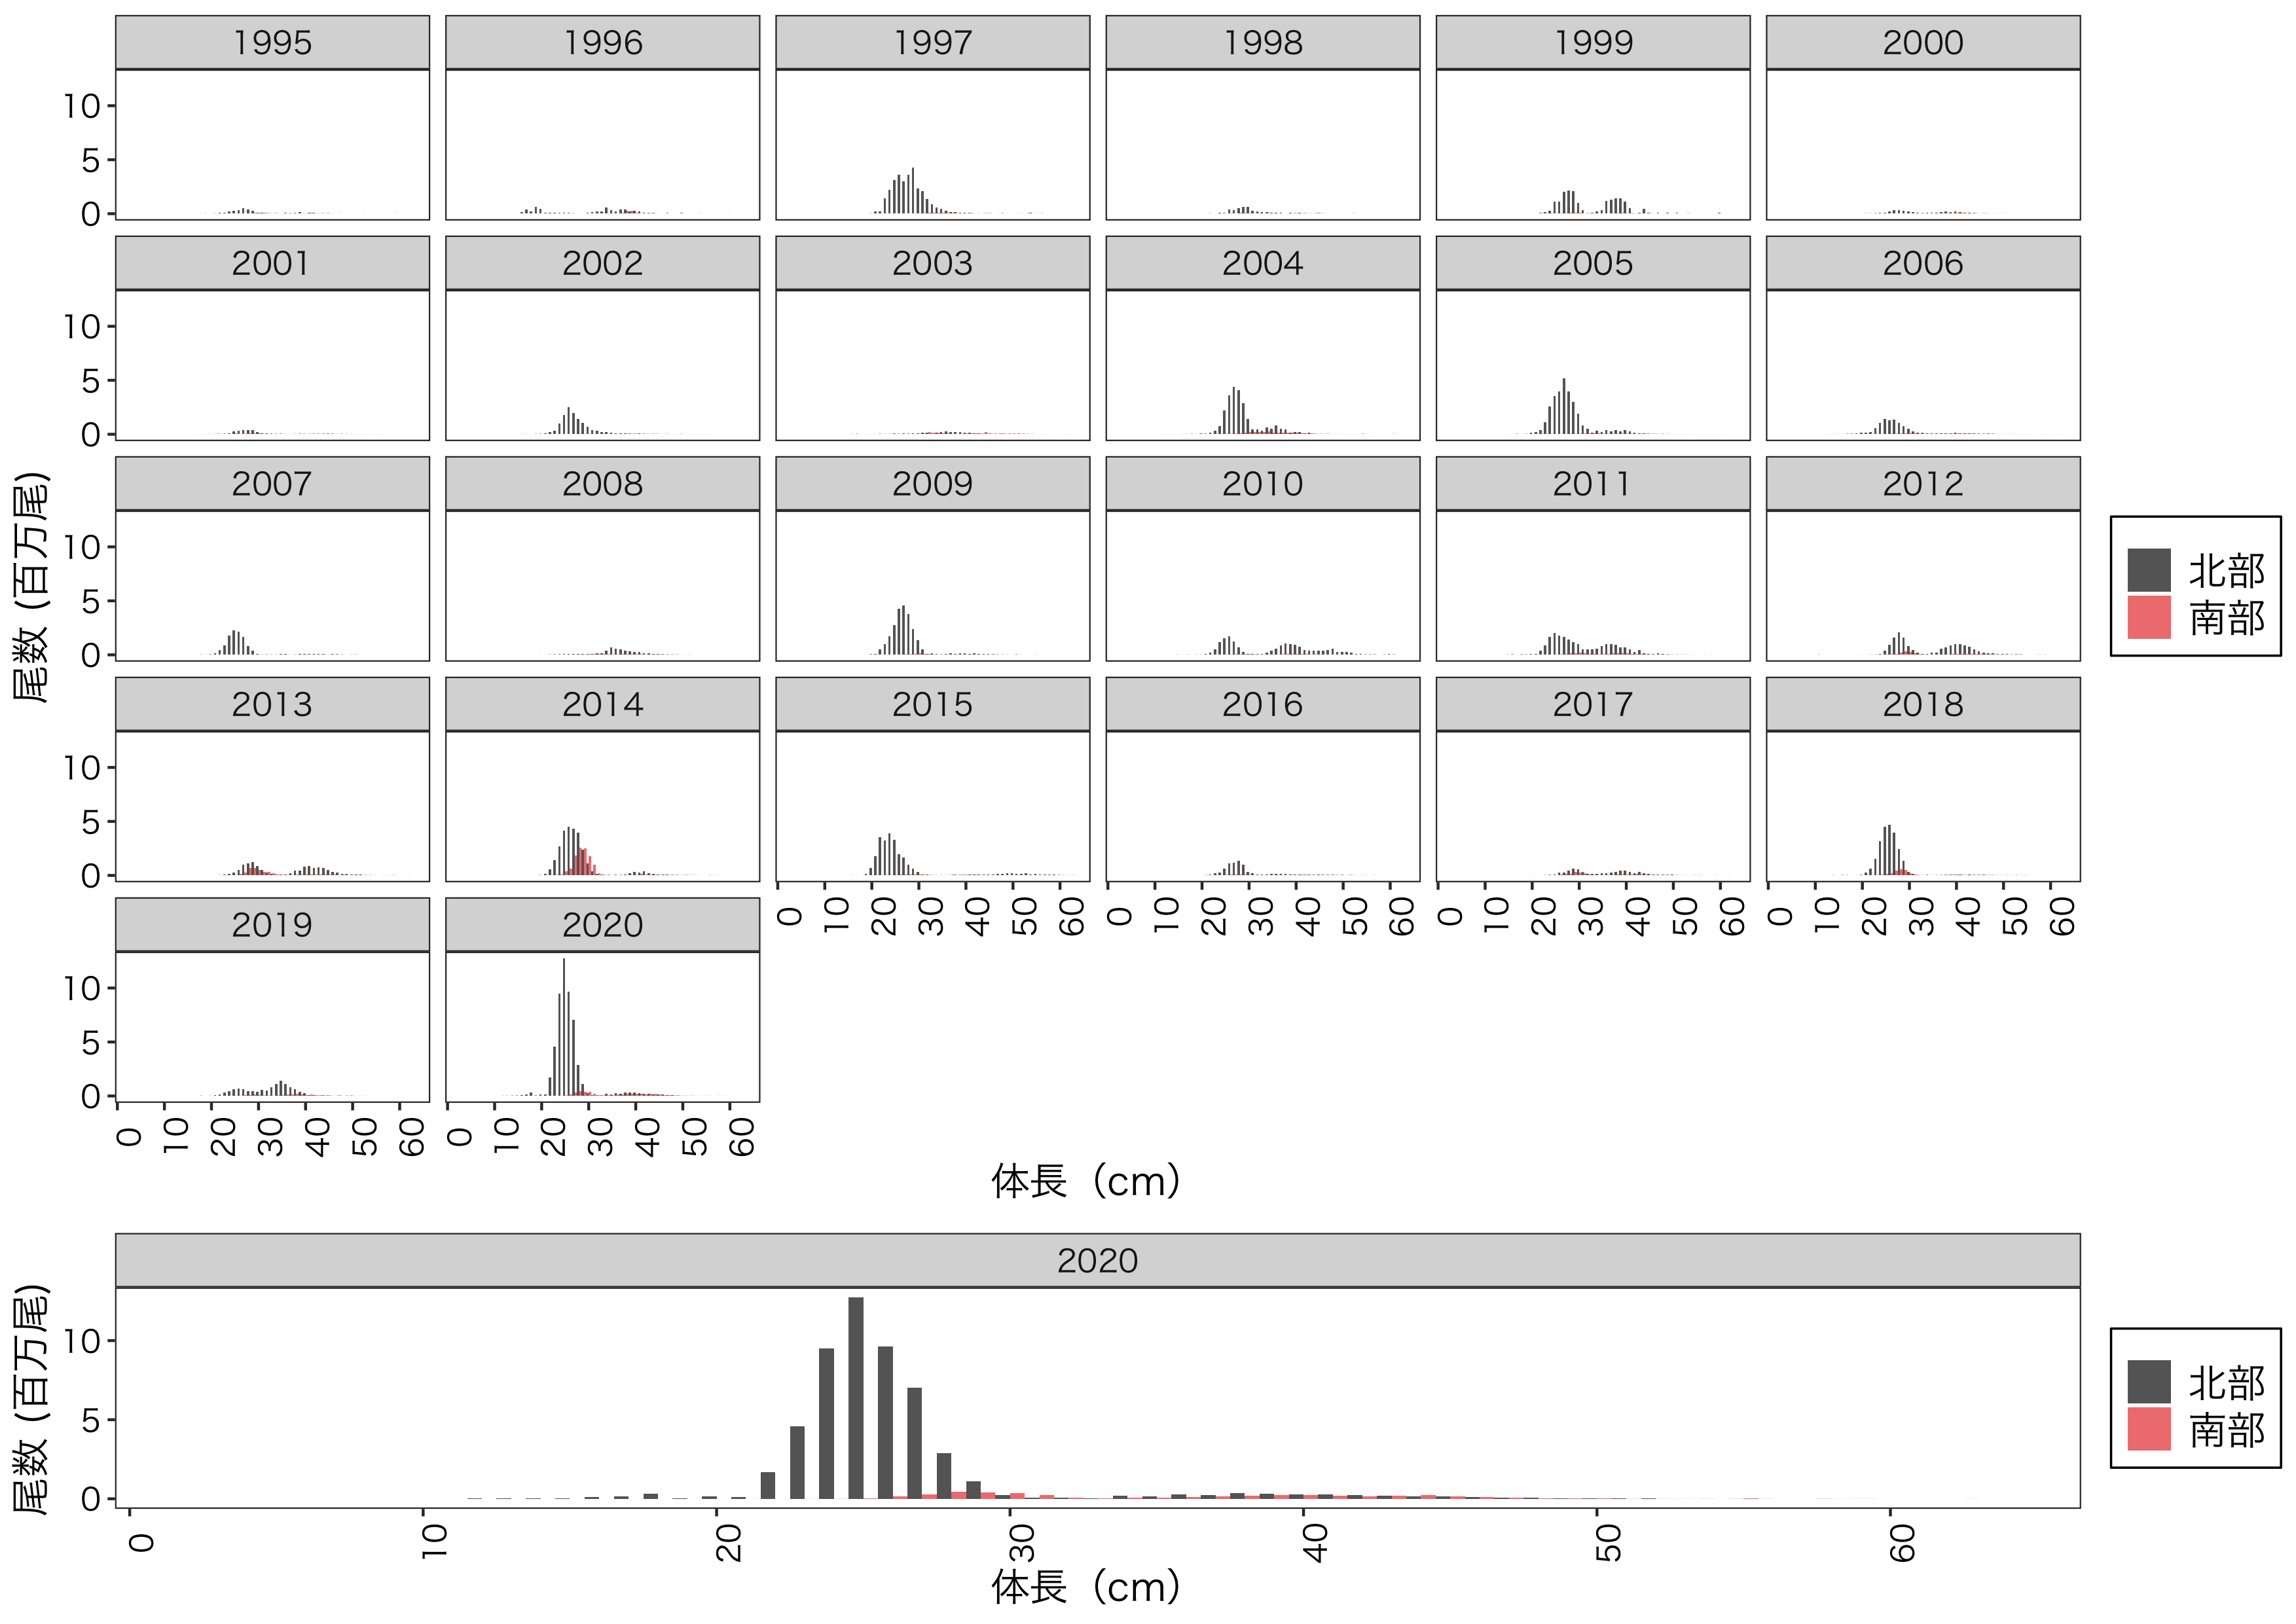
\includegraphics[width = 14cm]{スケトウダラ1+length.png}
  \caption{スケトウダラ1歳魚以上の体長組成の経年変化}
\end{figure}

\begin{figure}[h]
  \centering
  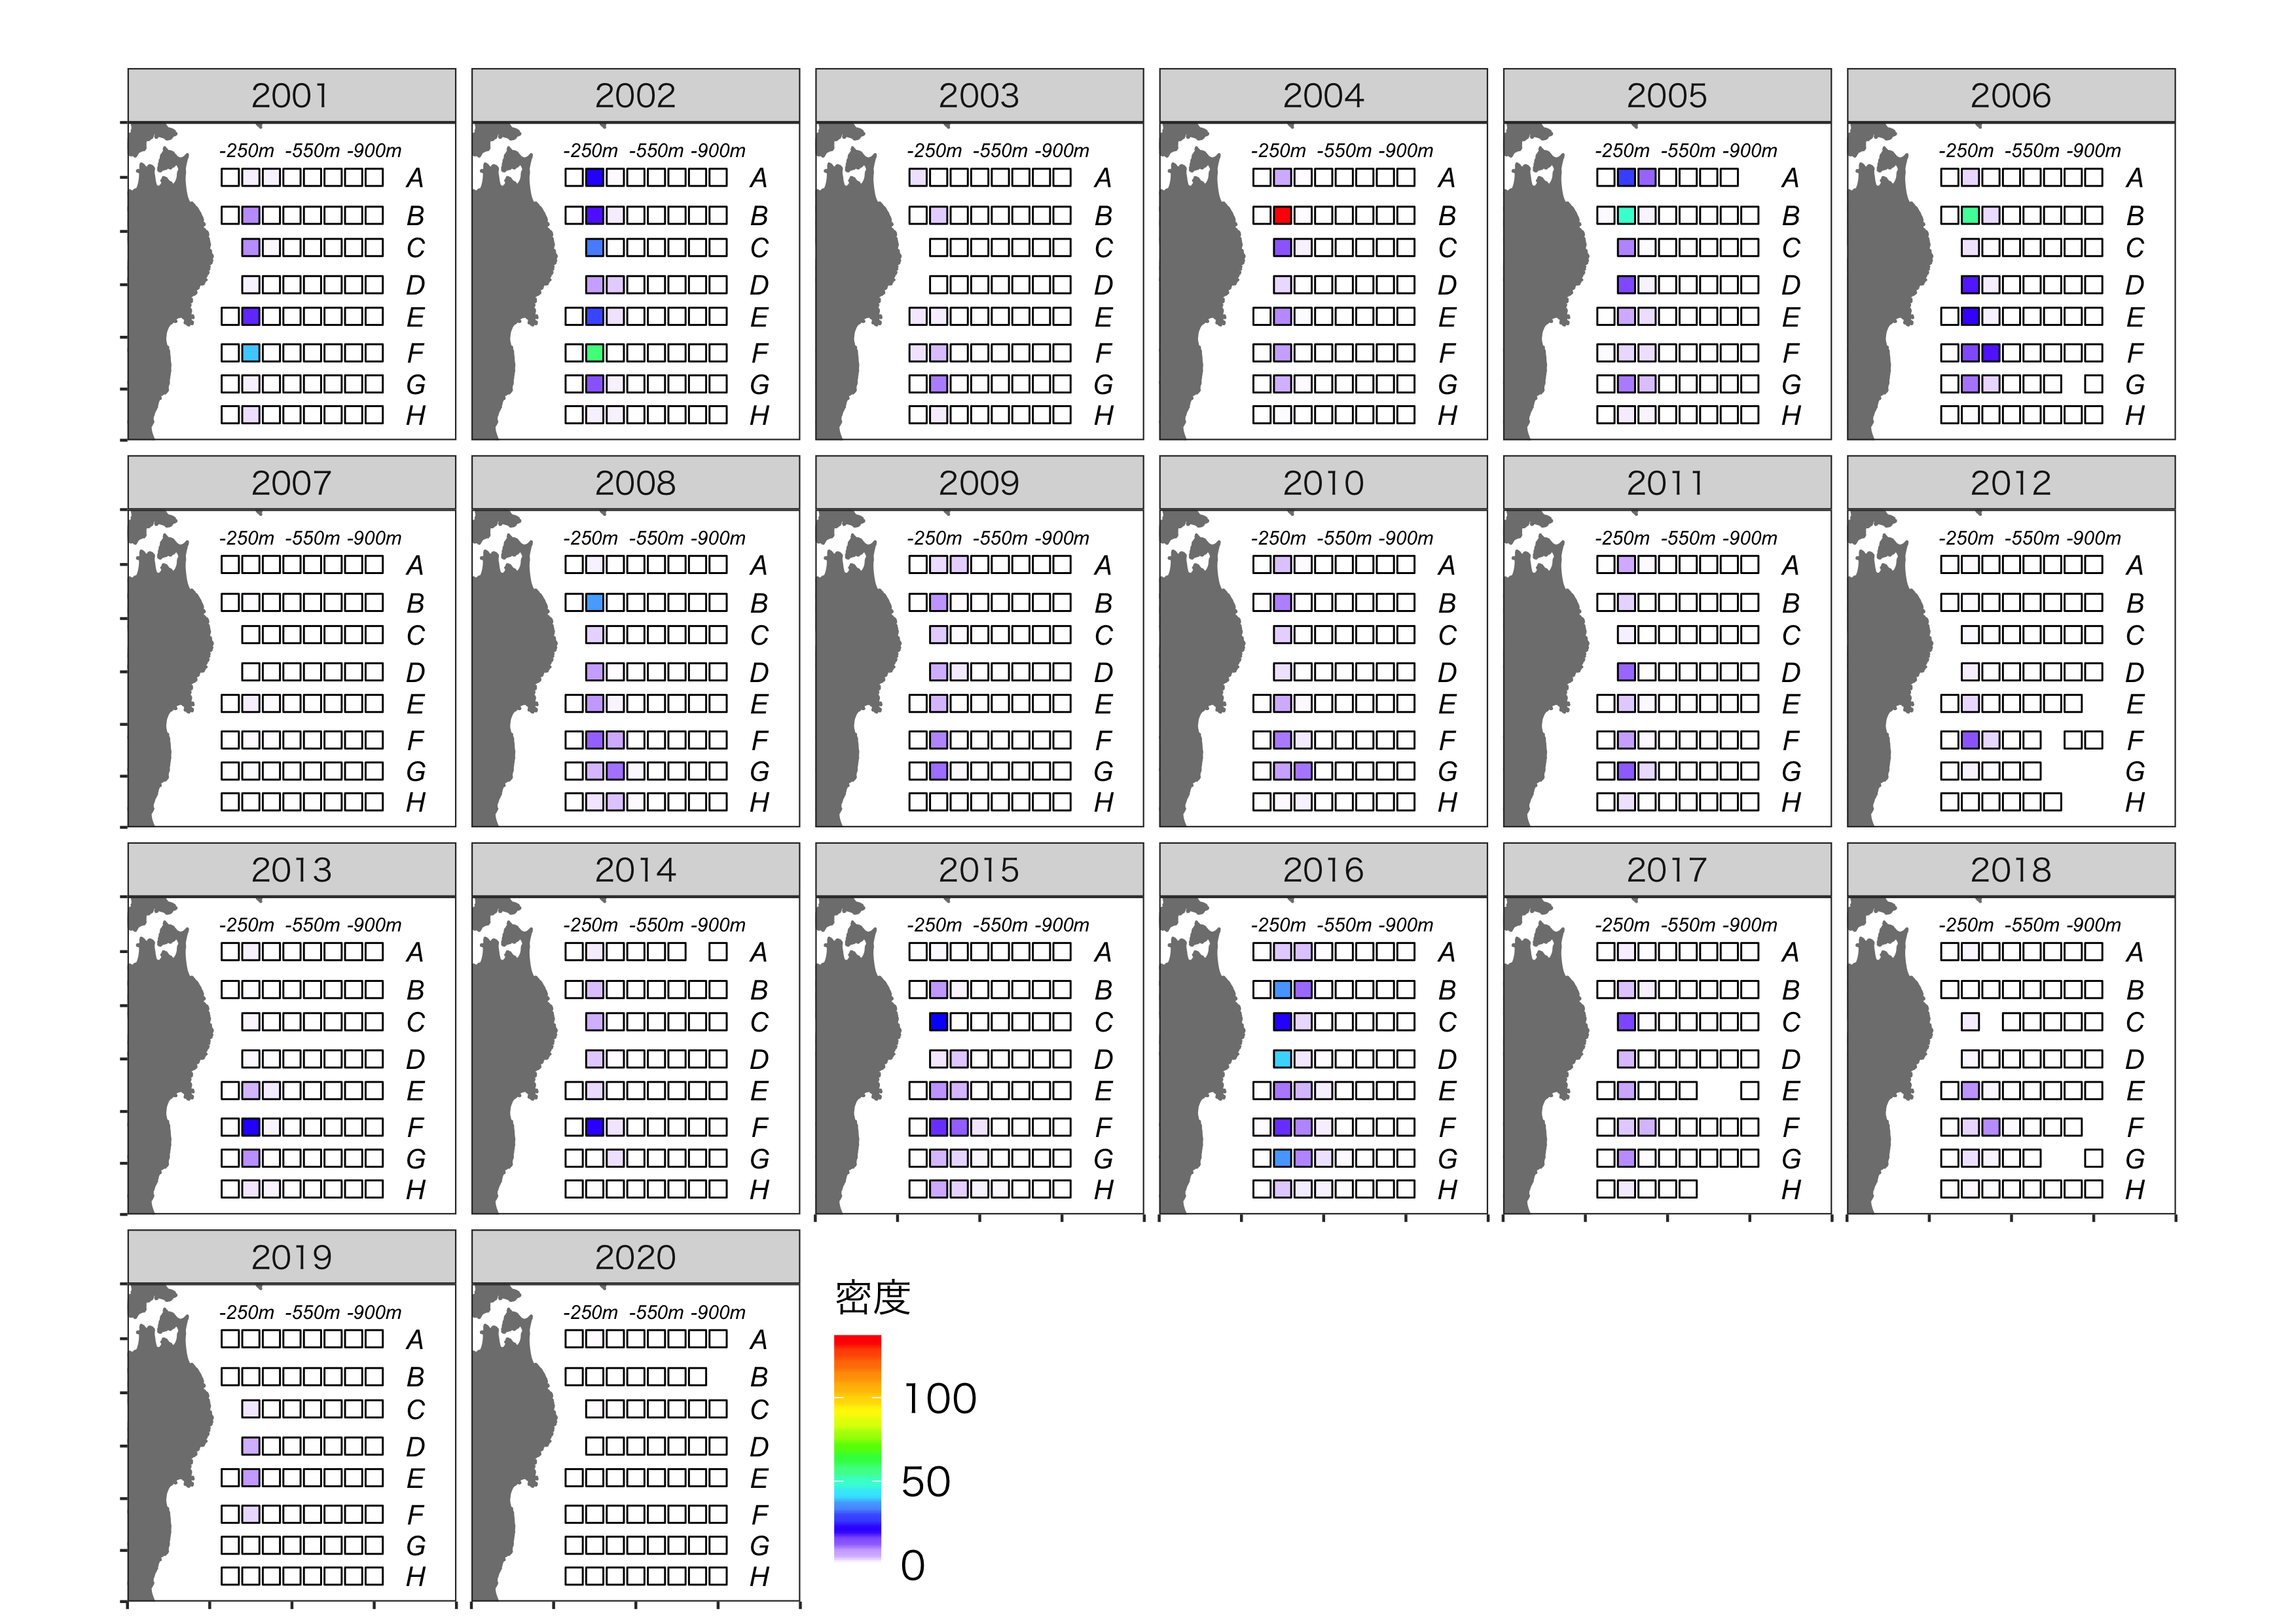
\includegraphics[width = 14cm]{マダラ0+dens.png}
  \caption{マダラ0歳魚の分布密度(千尾/km2)の経年変化}
\end{figure}

\begin{figure}[h]
  \centering
  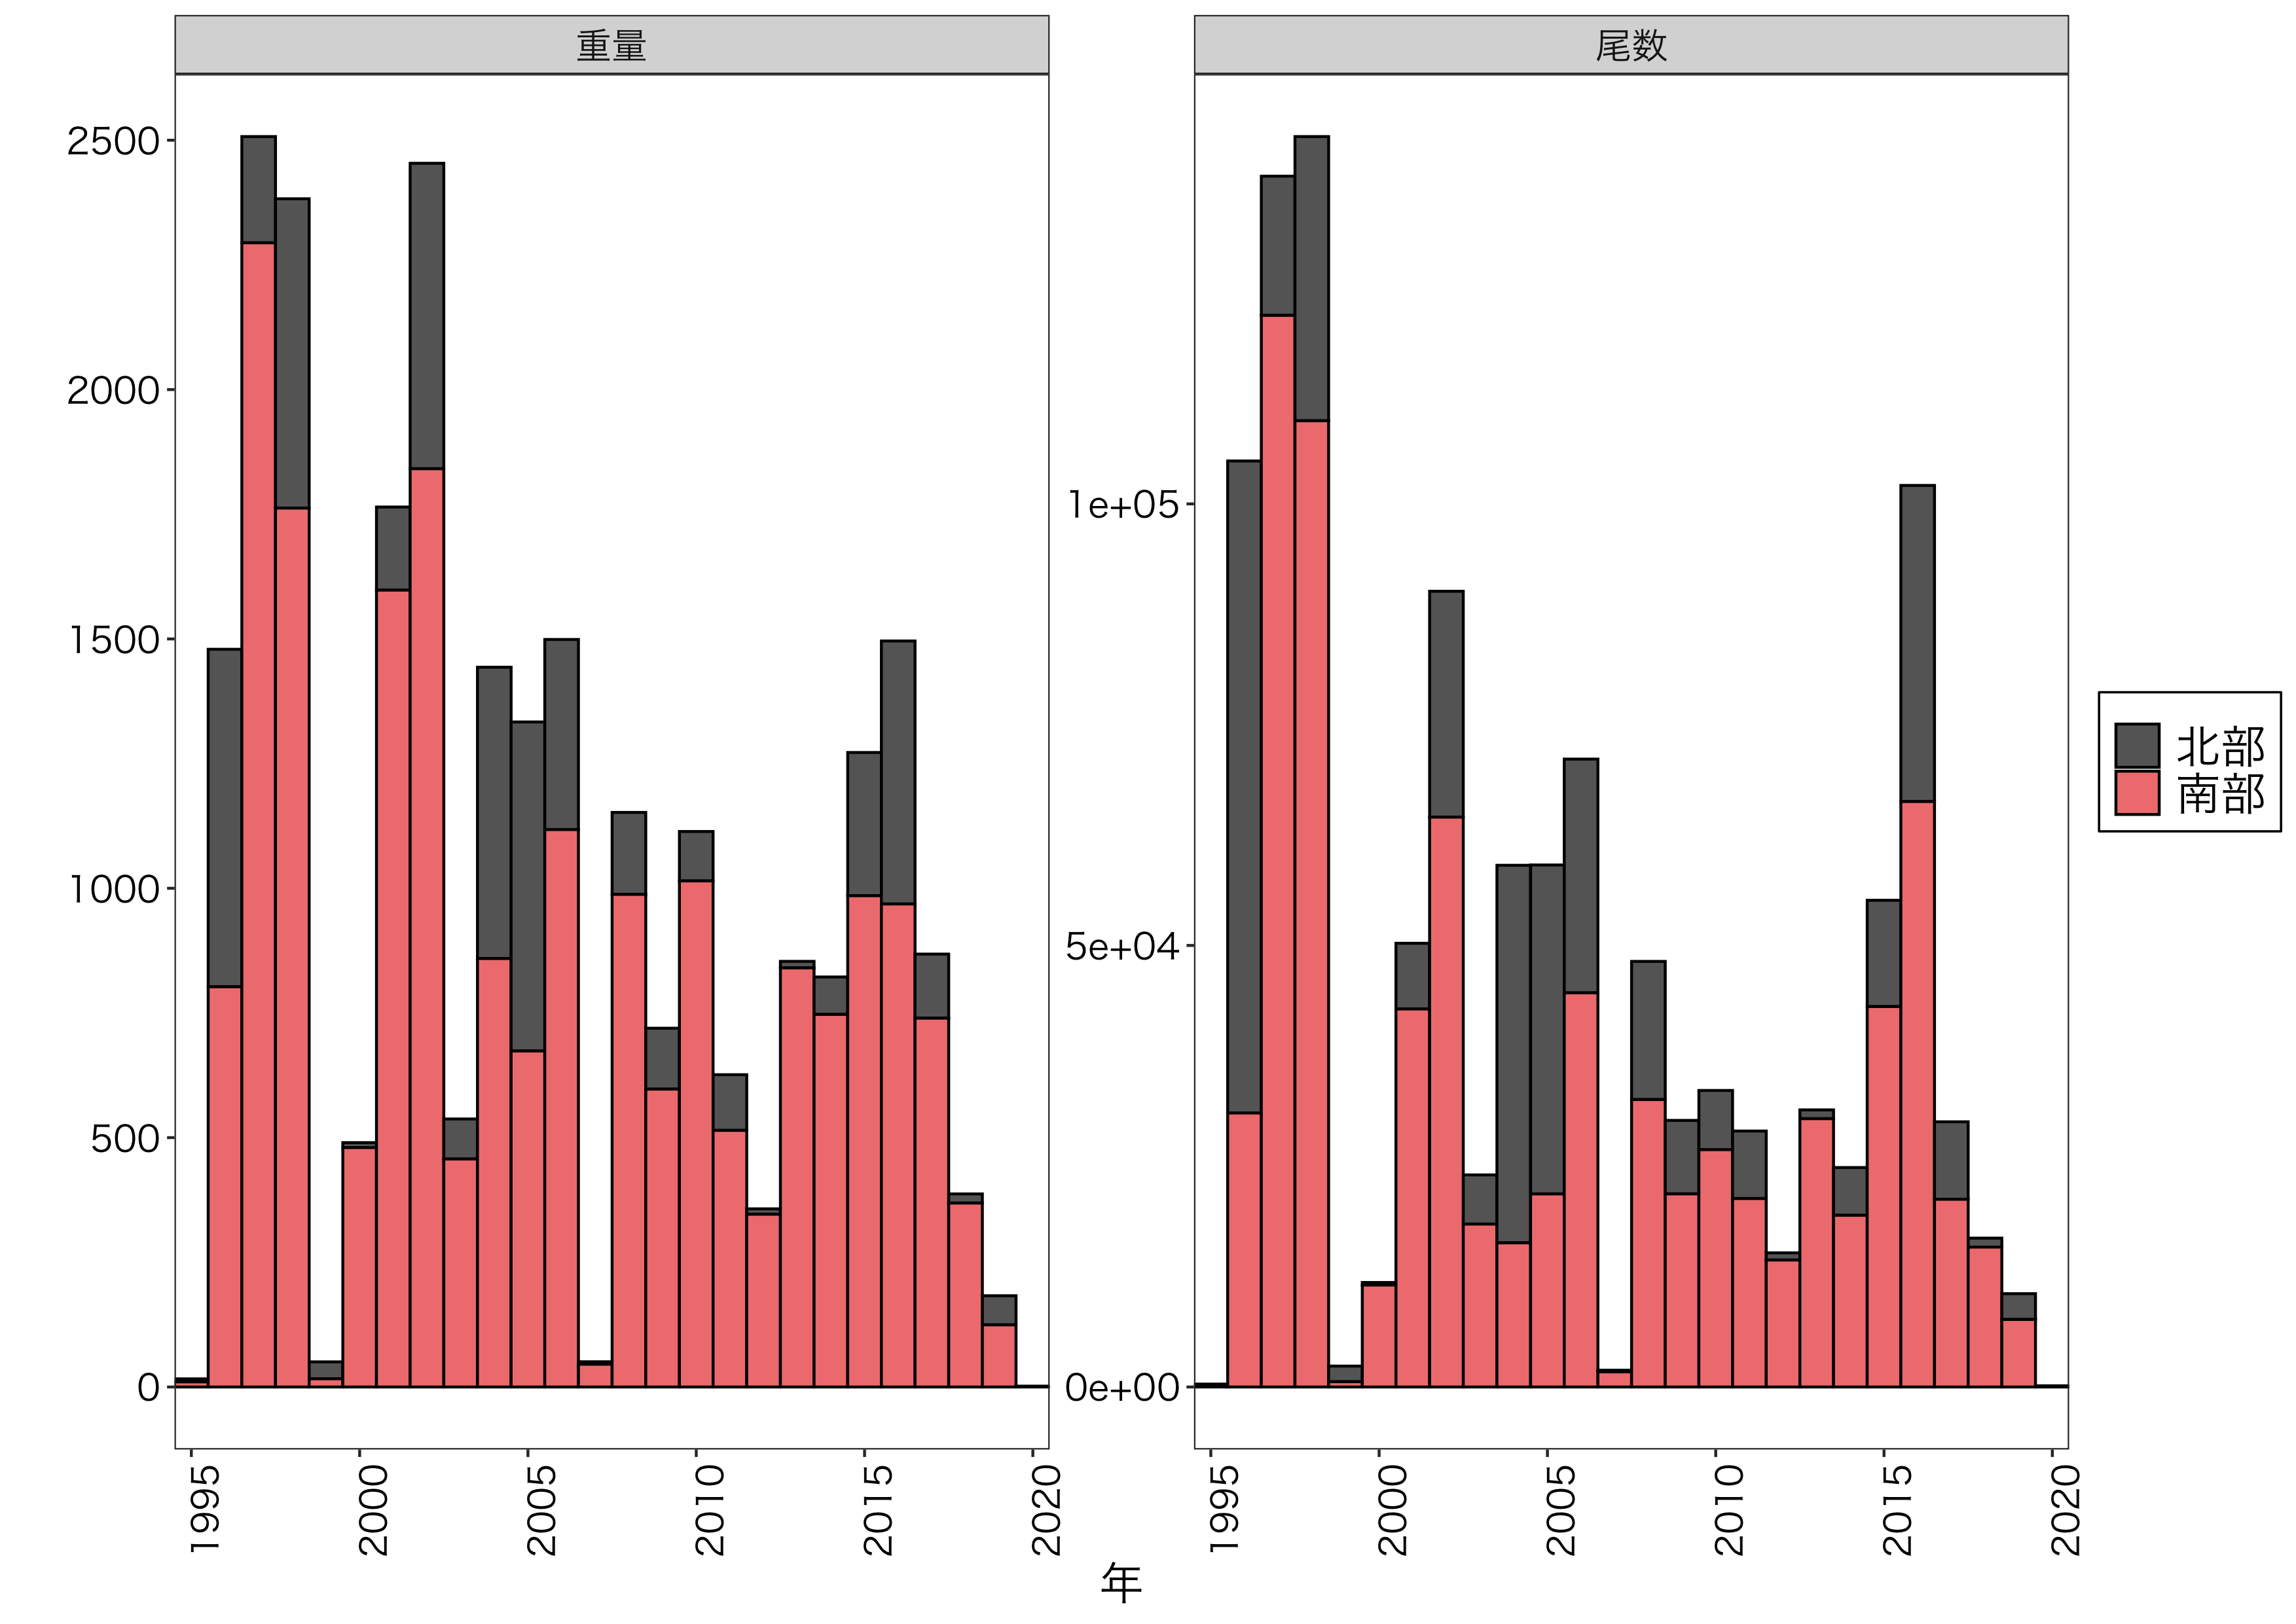
\includegraphics[width = 14cm]{マダラ0+trend.png}
  \caption{マダラ0歳魚の現存量(右; 単位は千トン)と現存尾数(左; 単位は百万尾)の経年変化}
\end{figure}

\begin{figure}[h]
  \centering
  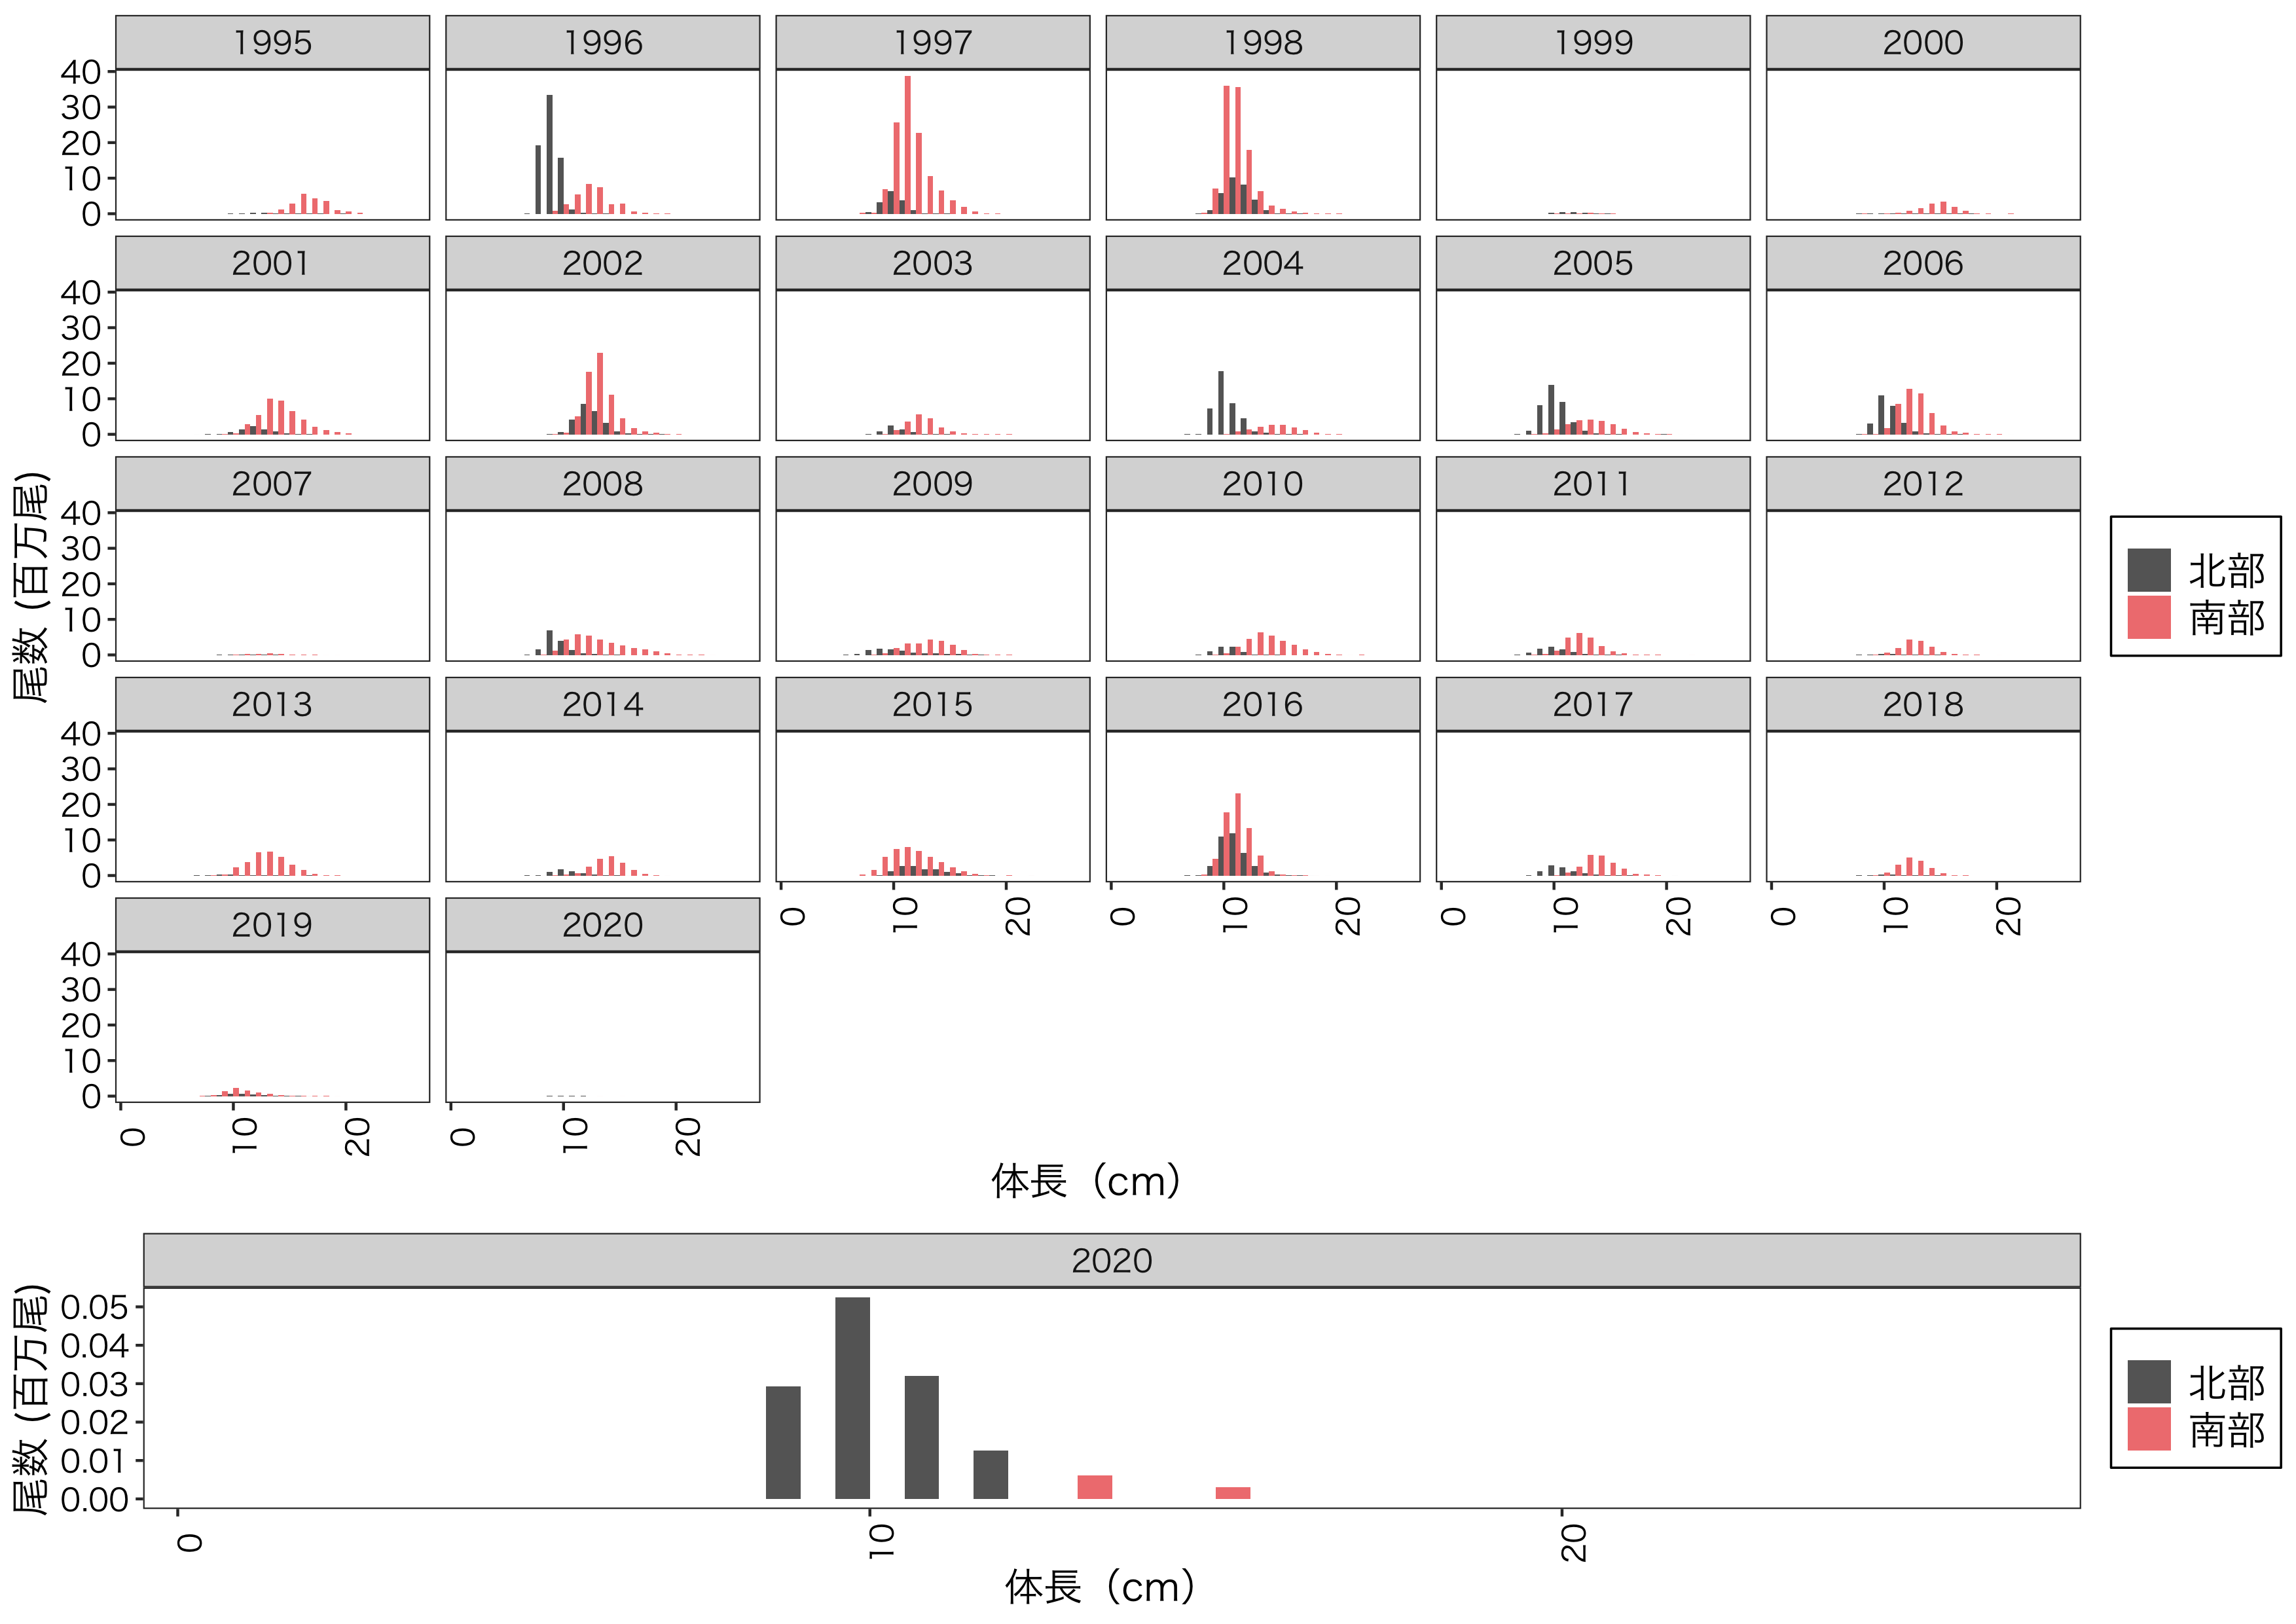
\includegraphics[width = 14cm]{マダラ0+length.png}
  \caption{マダラ0歳魚の体長組成の経年変化}
\end{figure}

\begin{figure}[h]
  \centering
  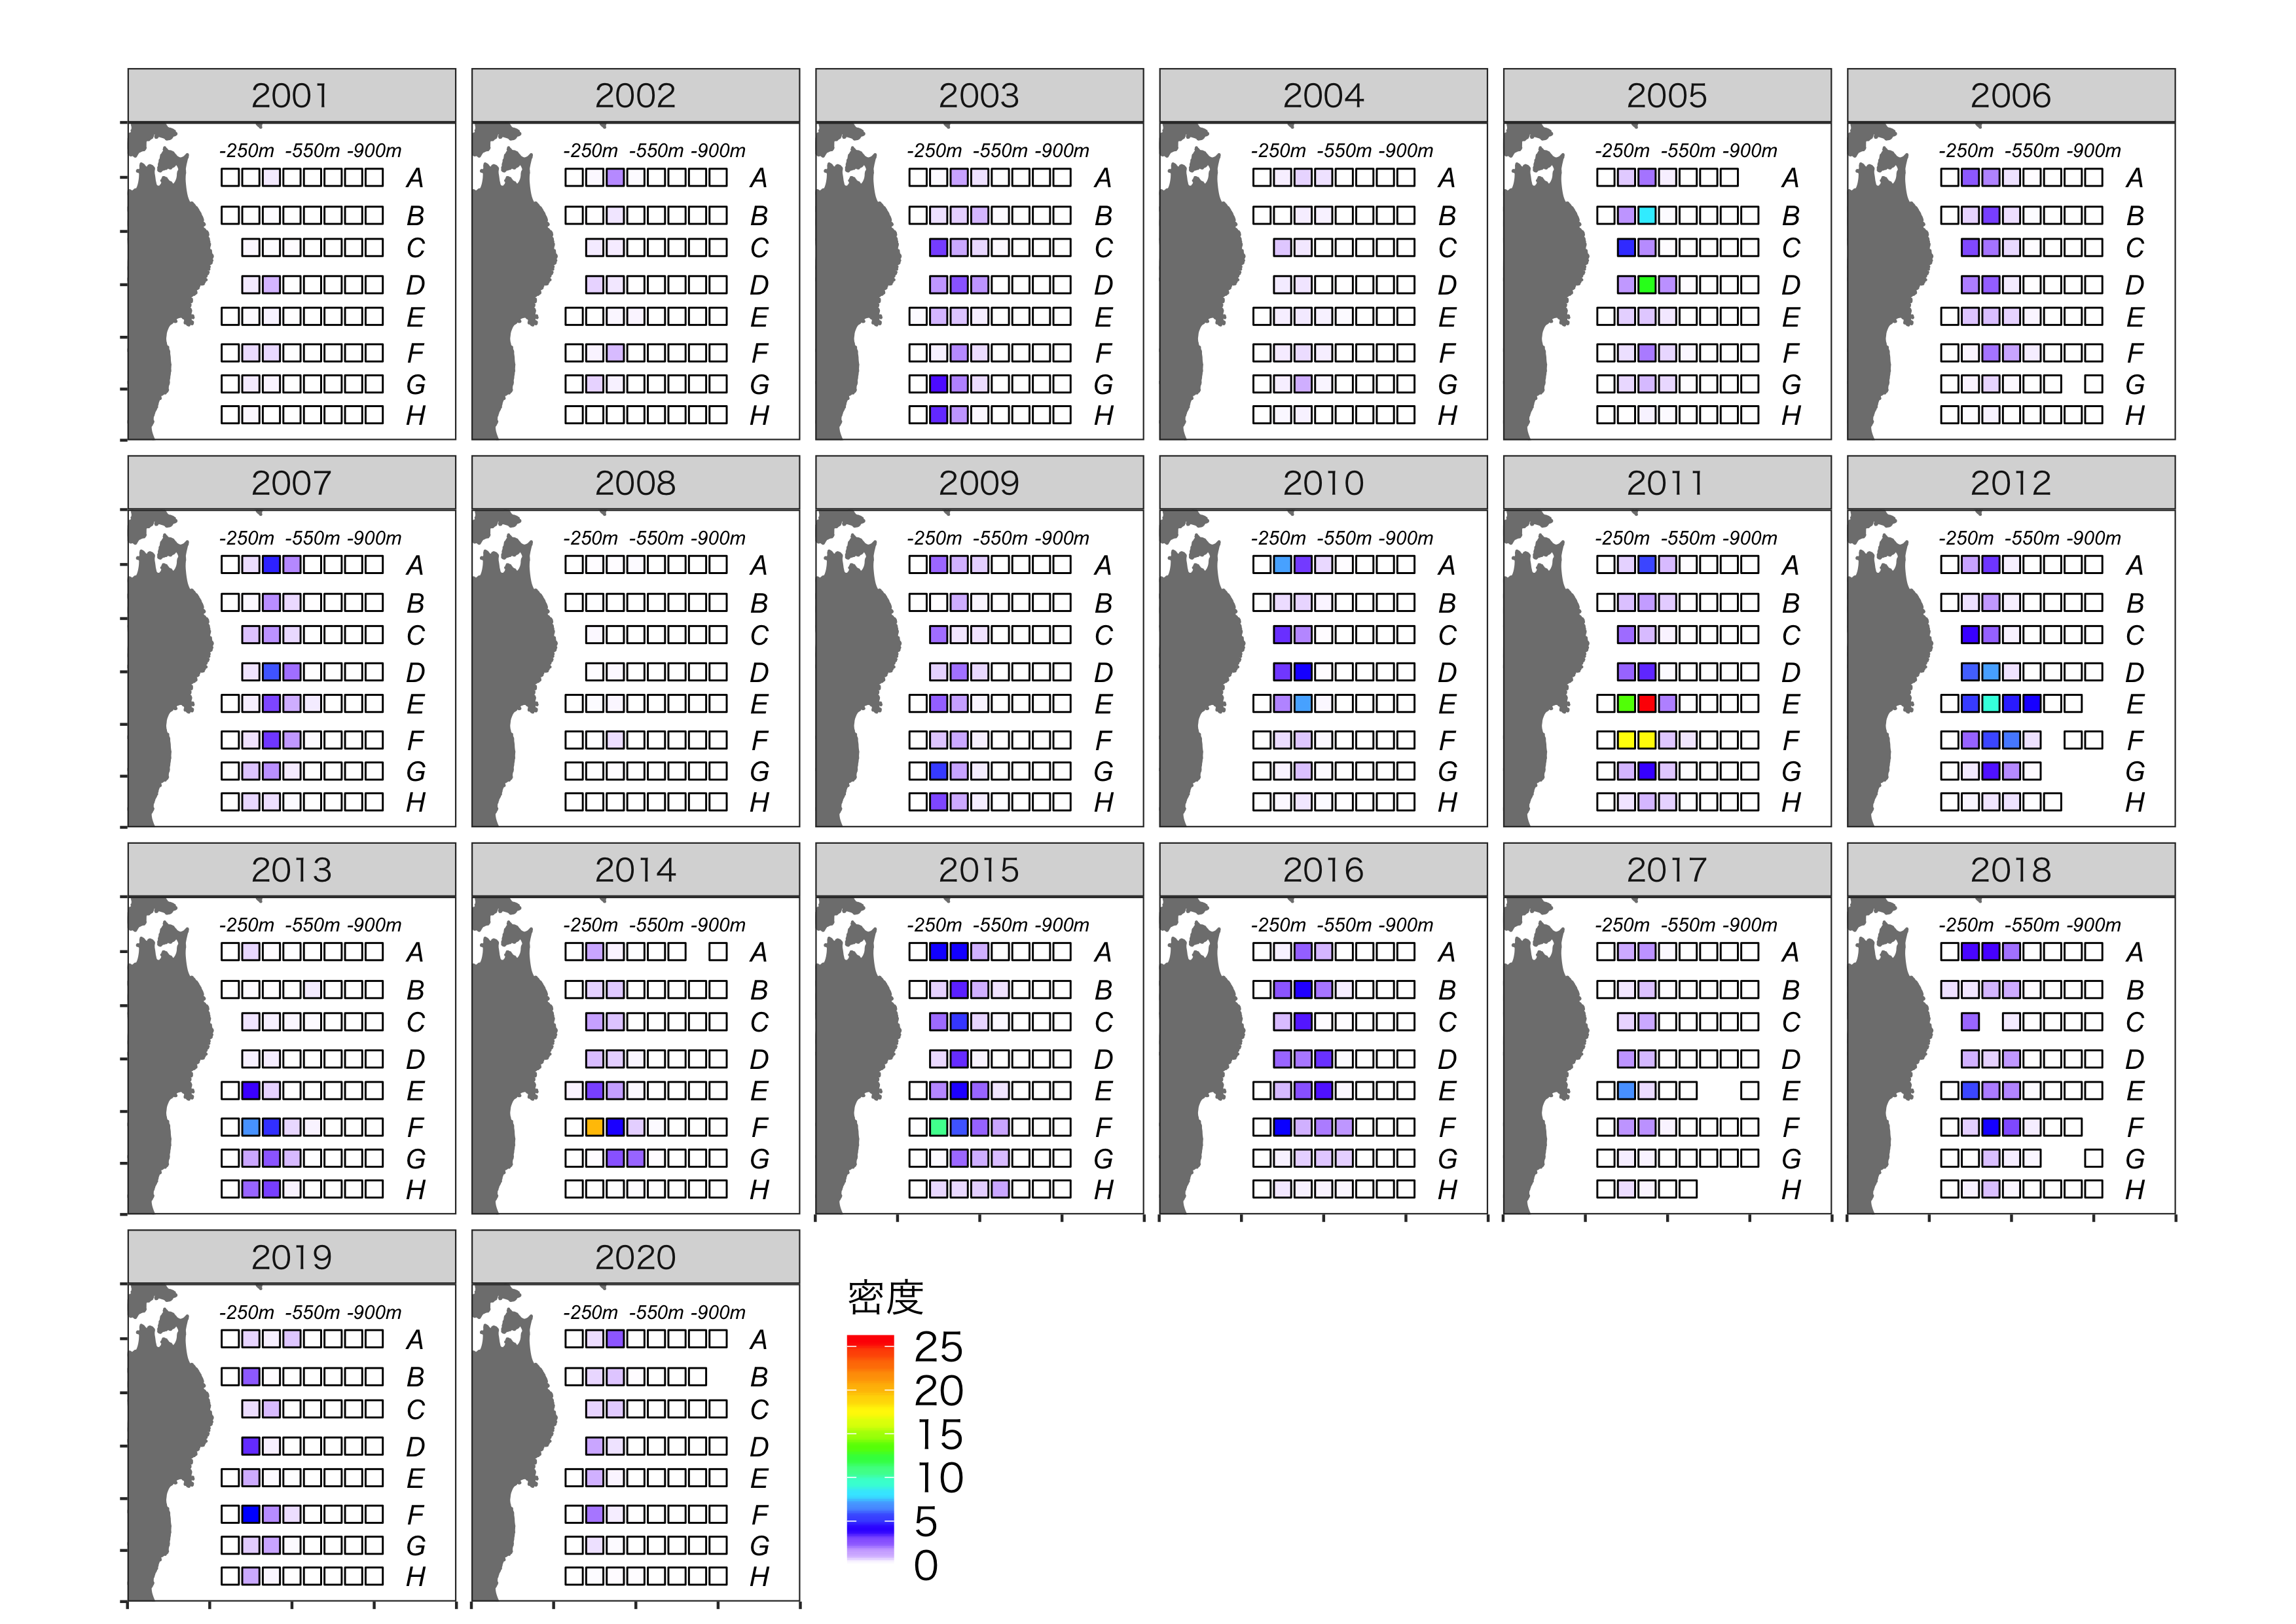
\includegraphics[width = 14cm]{マダラ1+dens.png}
  \caption{マダラ1歳魚の分布密度(千尾/km2)の経年変化}
\end{figure}

\begin{figure}[h]
  \centering
  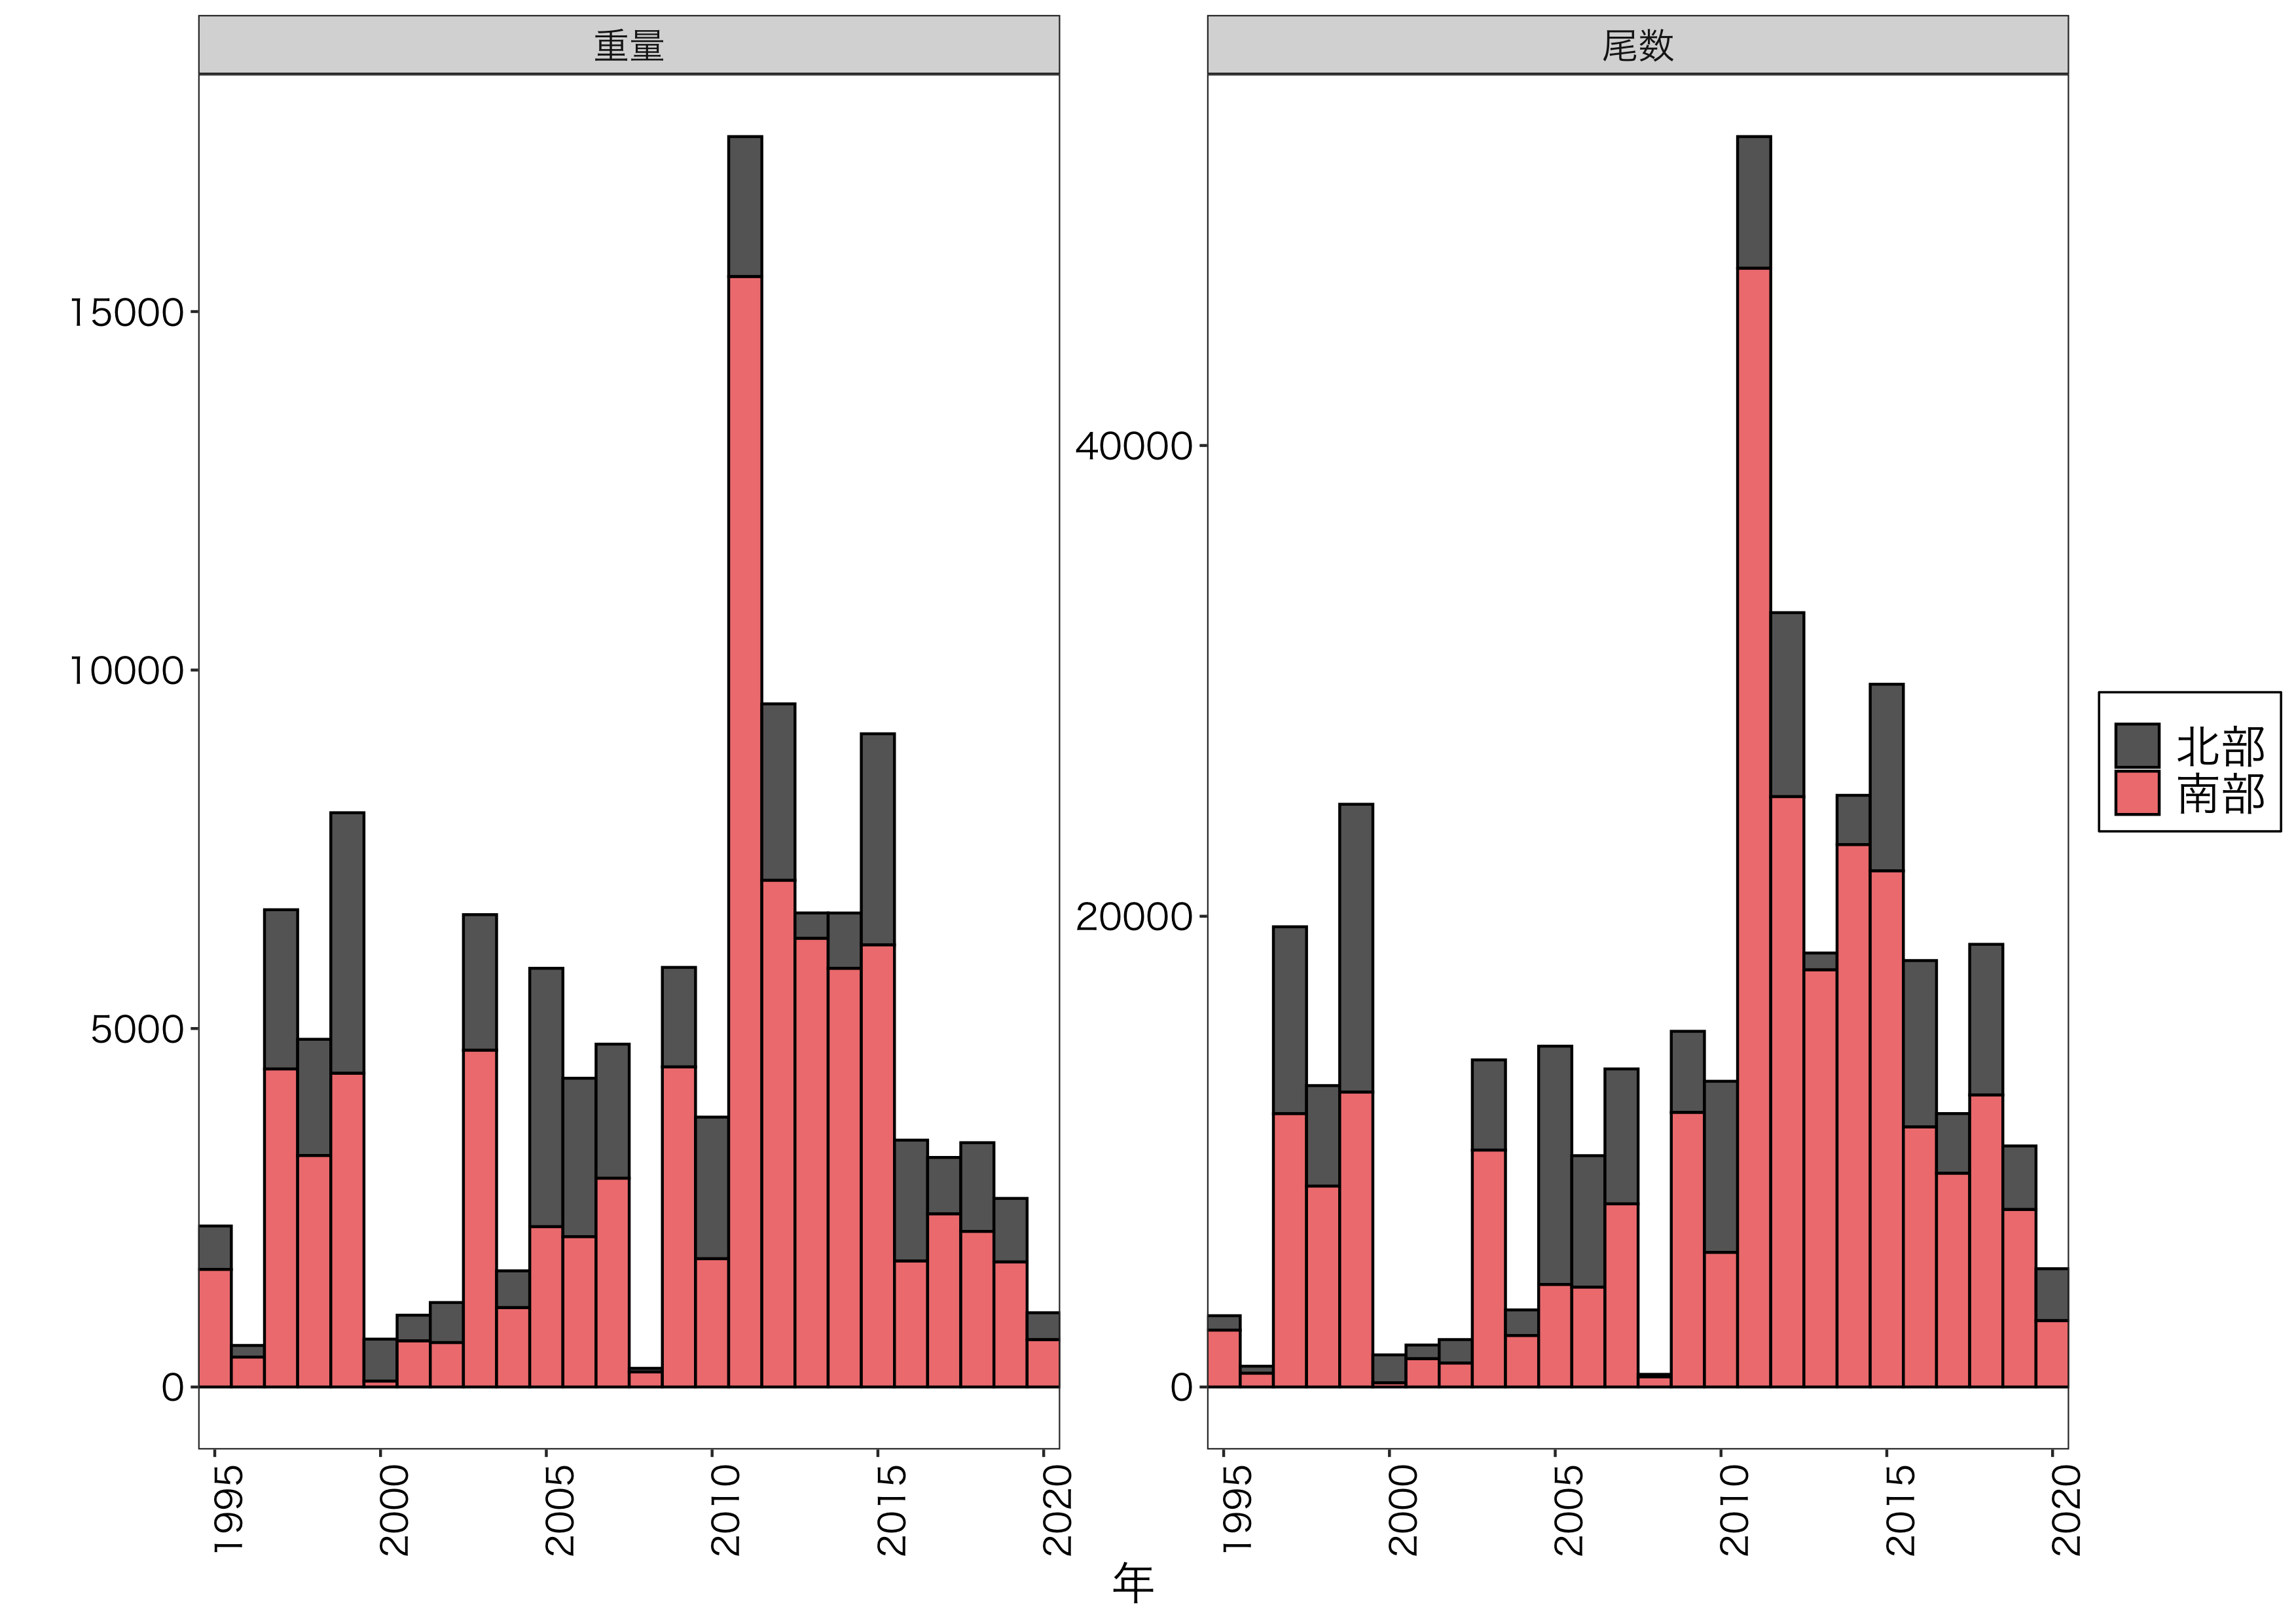
\includegraphics[width = 14cm]{マダラ1+trend.png}
  \caption{マダラ1歳魚の現存量(右; 単位は千トン)と現存尾数(左; 単位は百万尾)の経年変化}
\end{figure}

\begin{figure}[h]
  \centering
  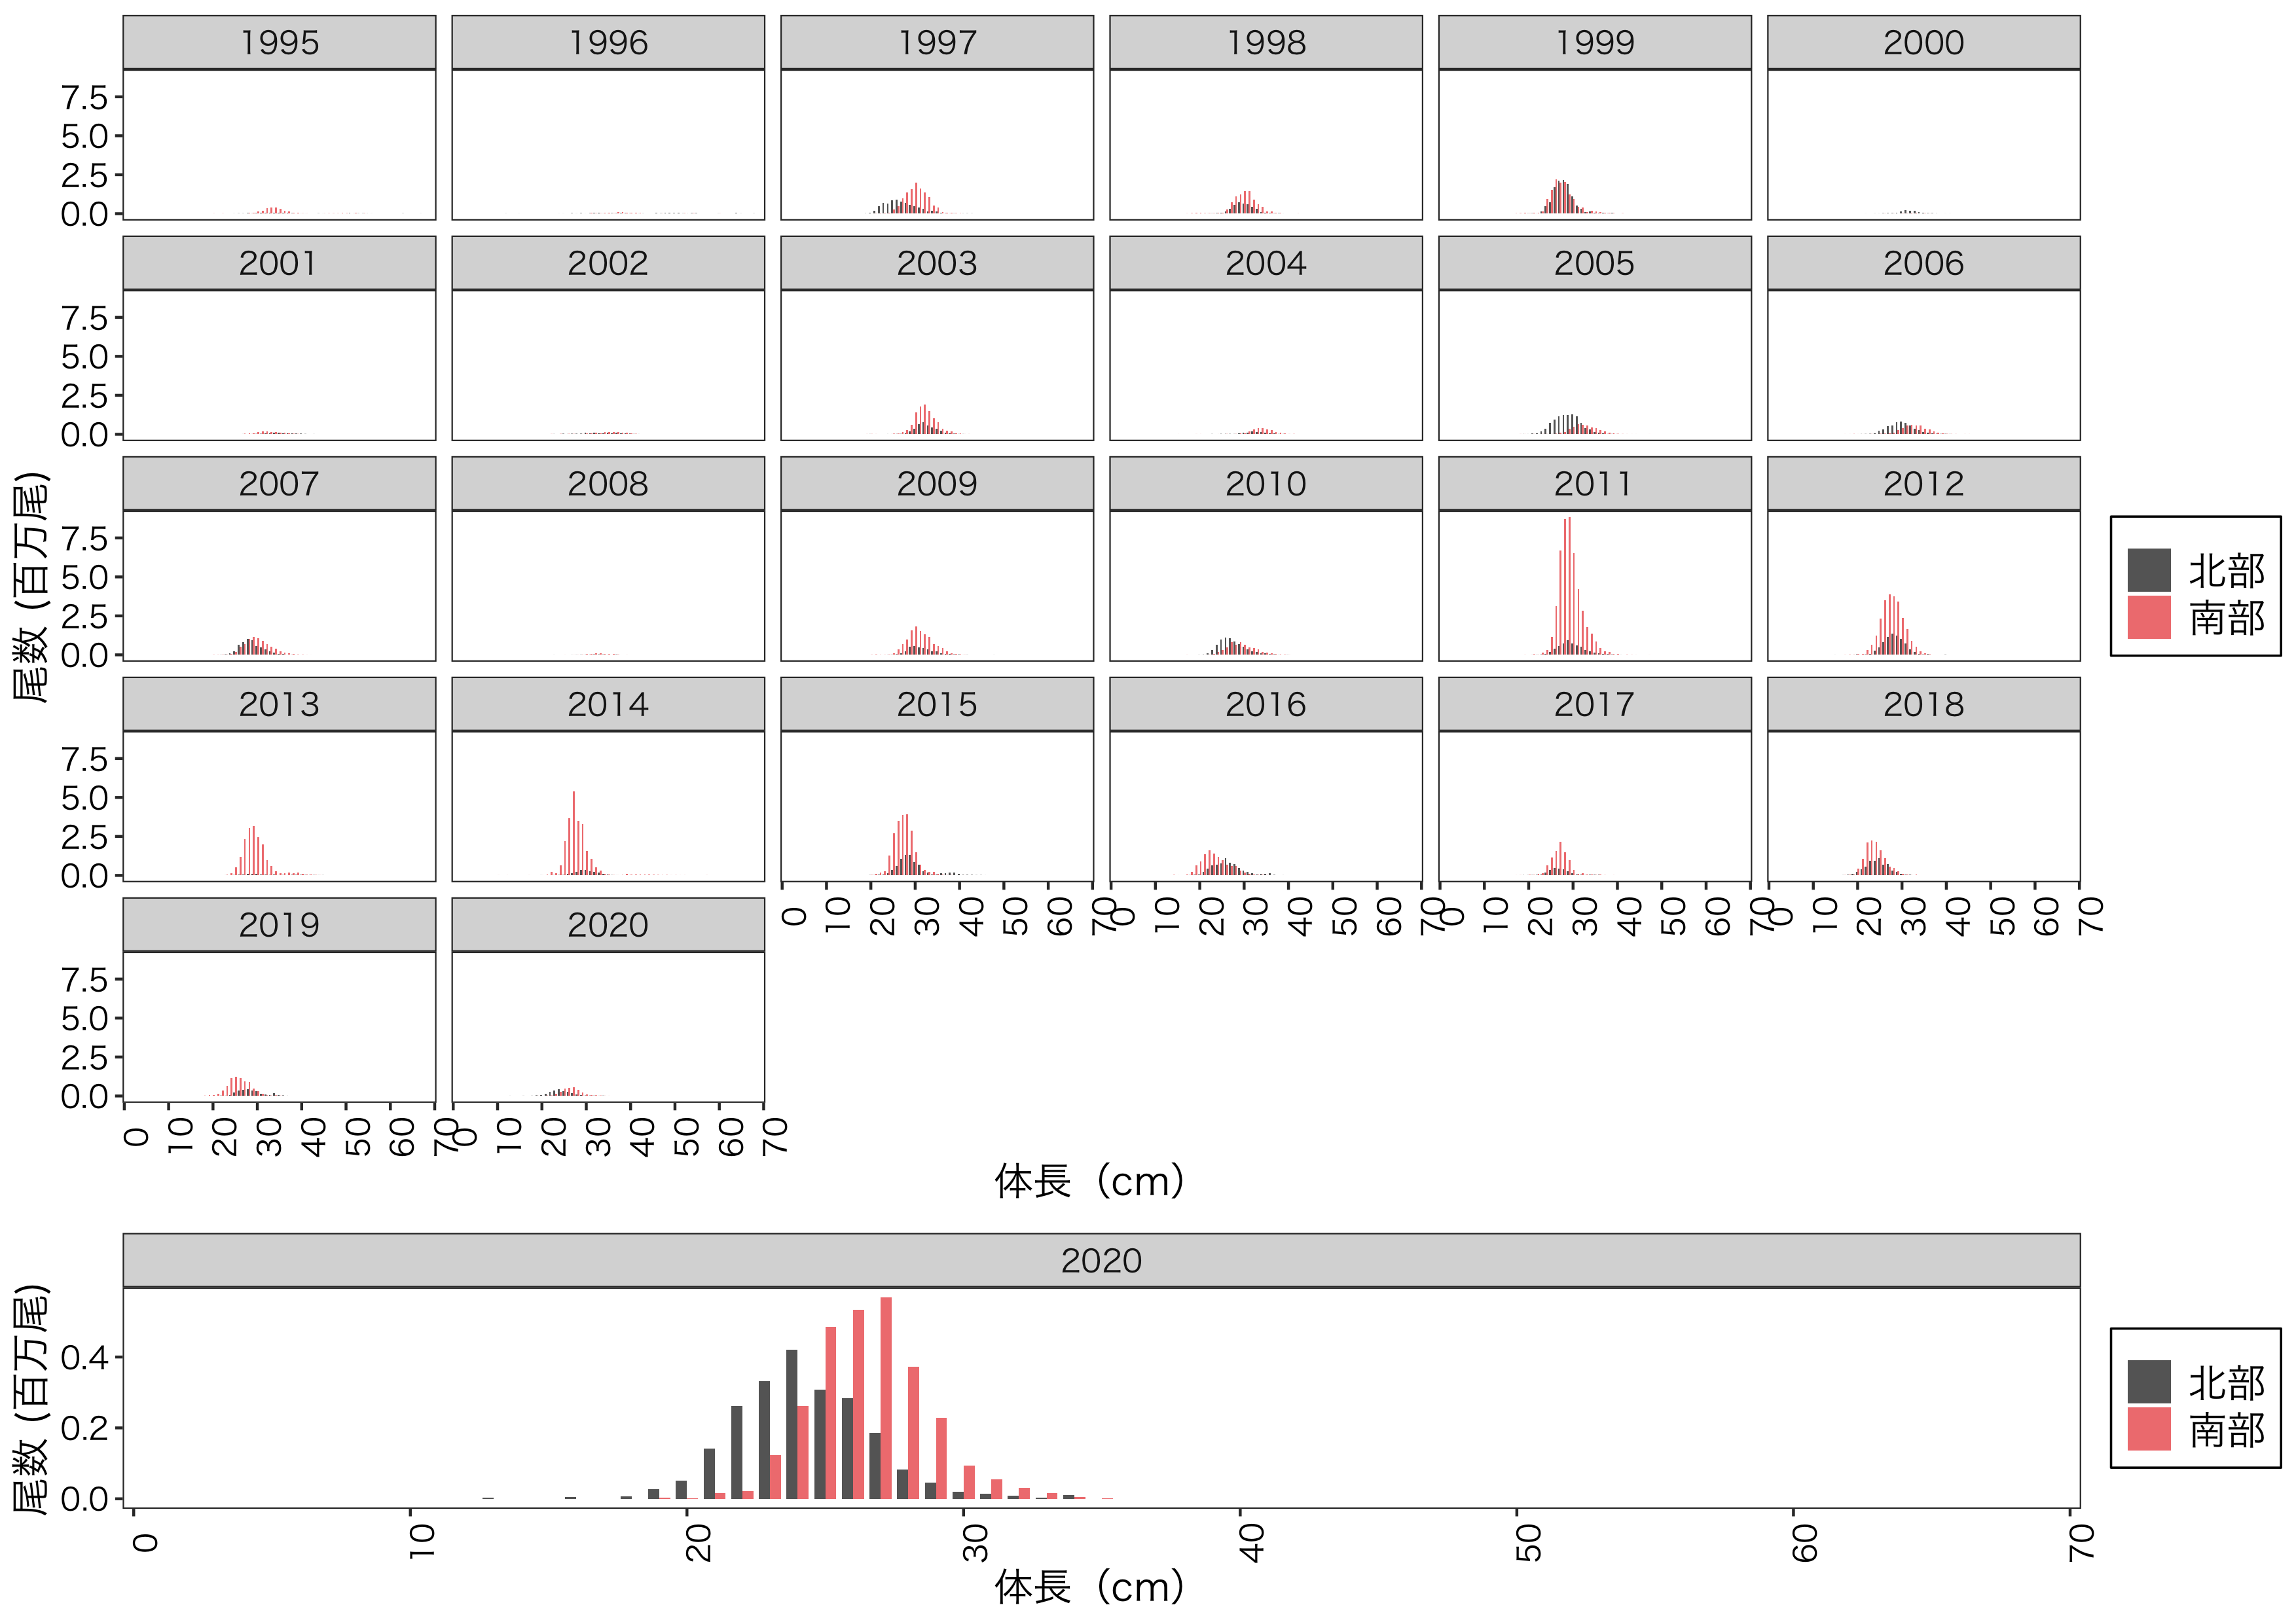
\includegraphics[width = 14cm]{マダラ1+length.png}
  \caption{マダラ1歳魚の体長組成の経年変化}
\end{figure}

\begin{figure}[h]
  \centering
  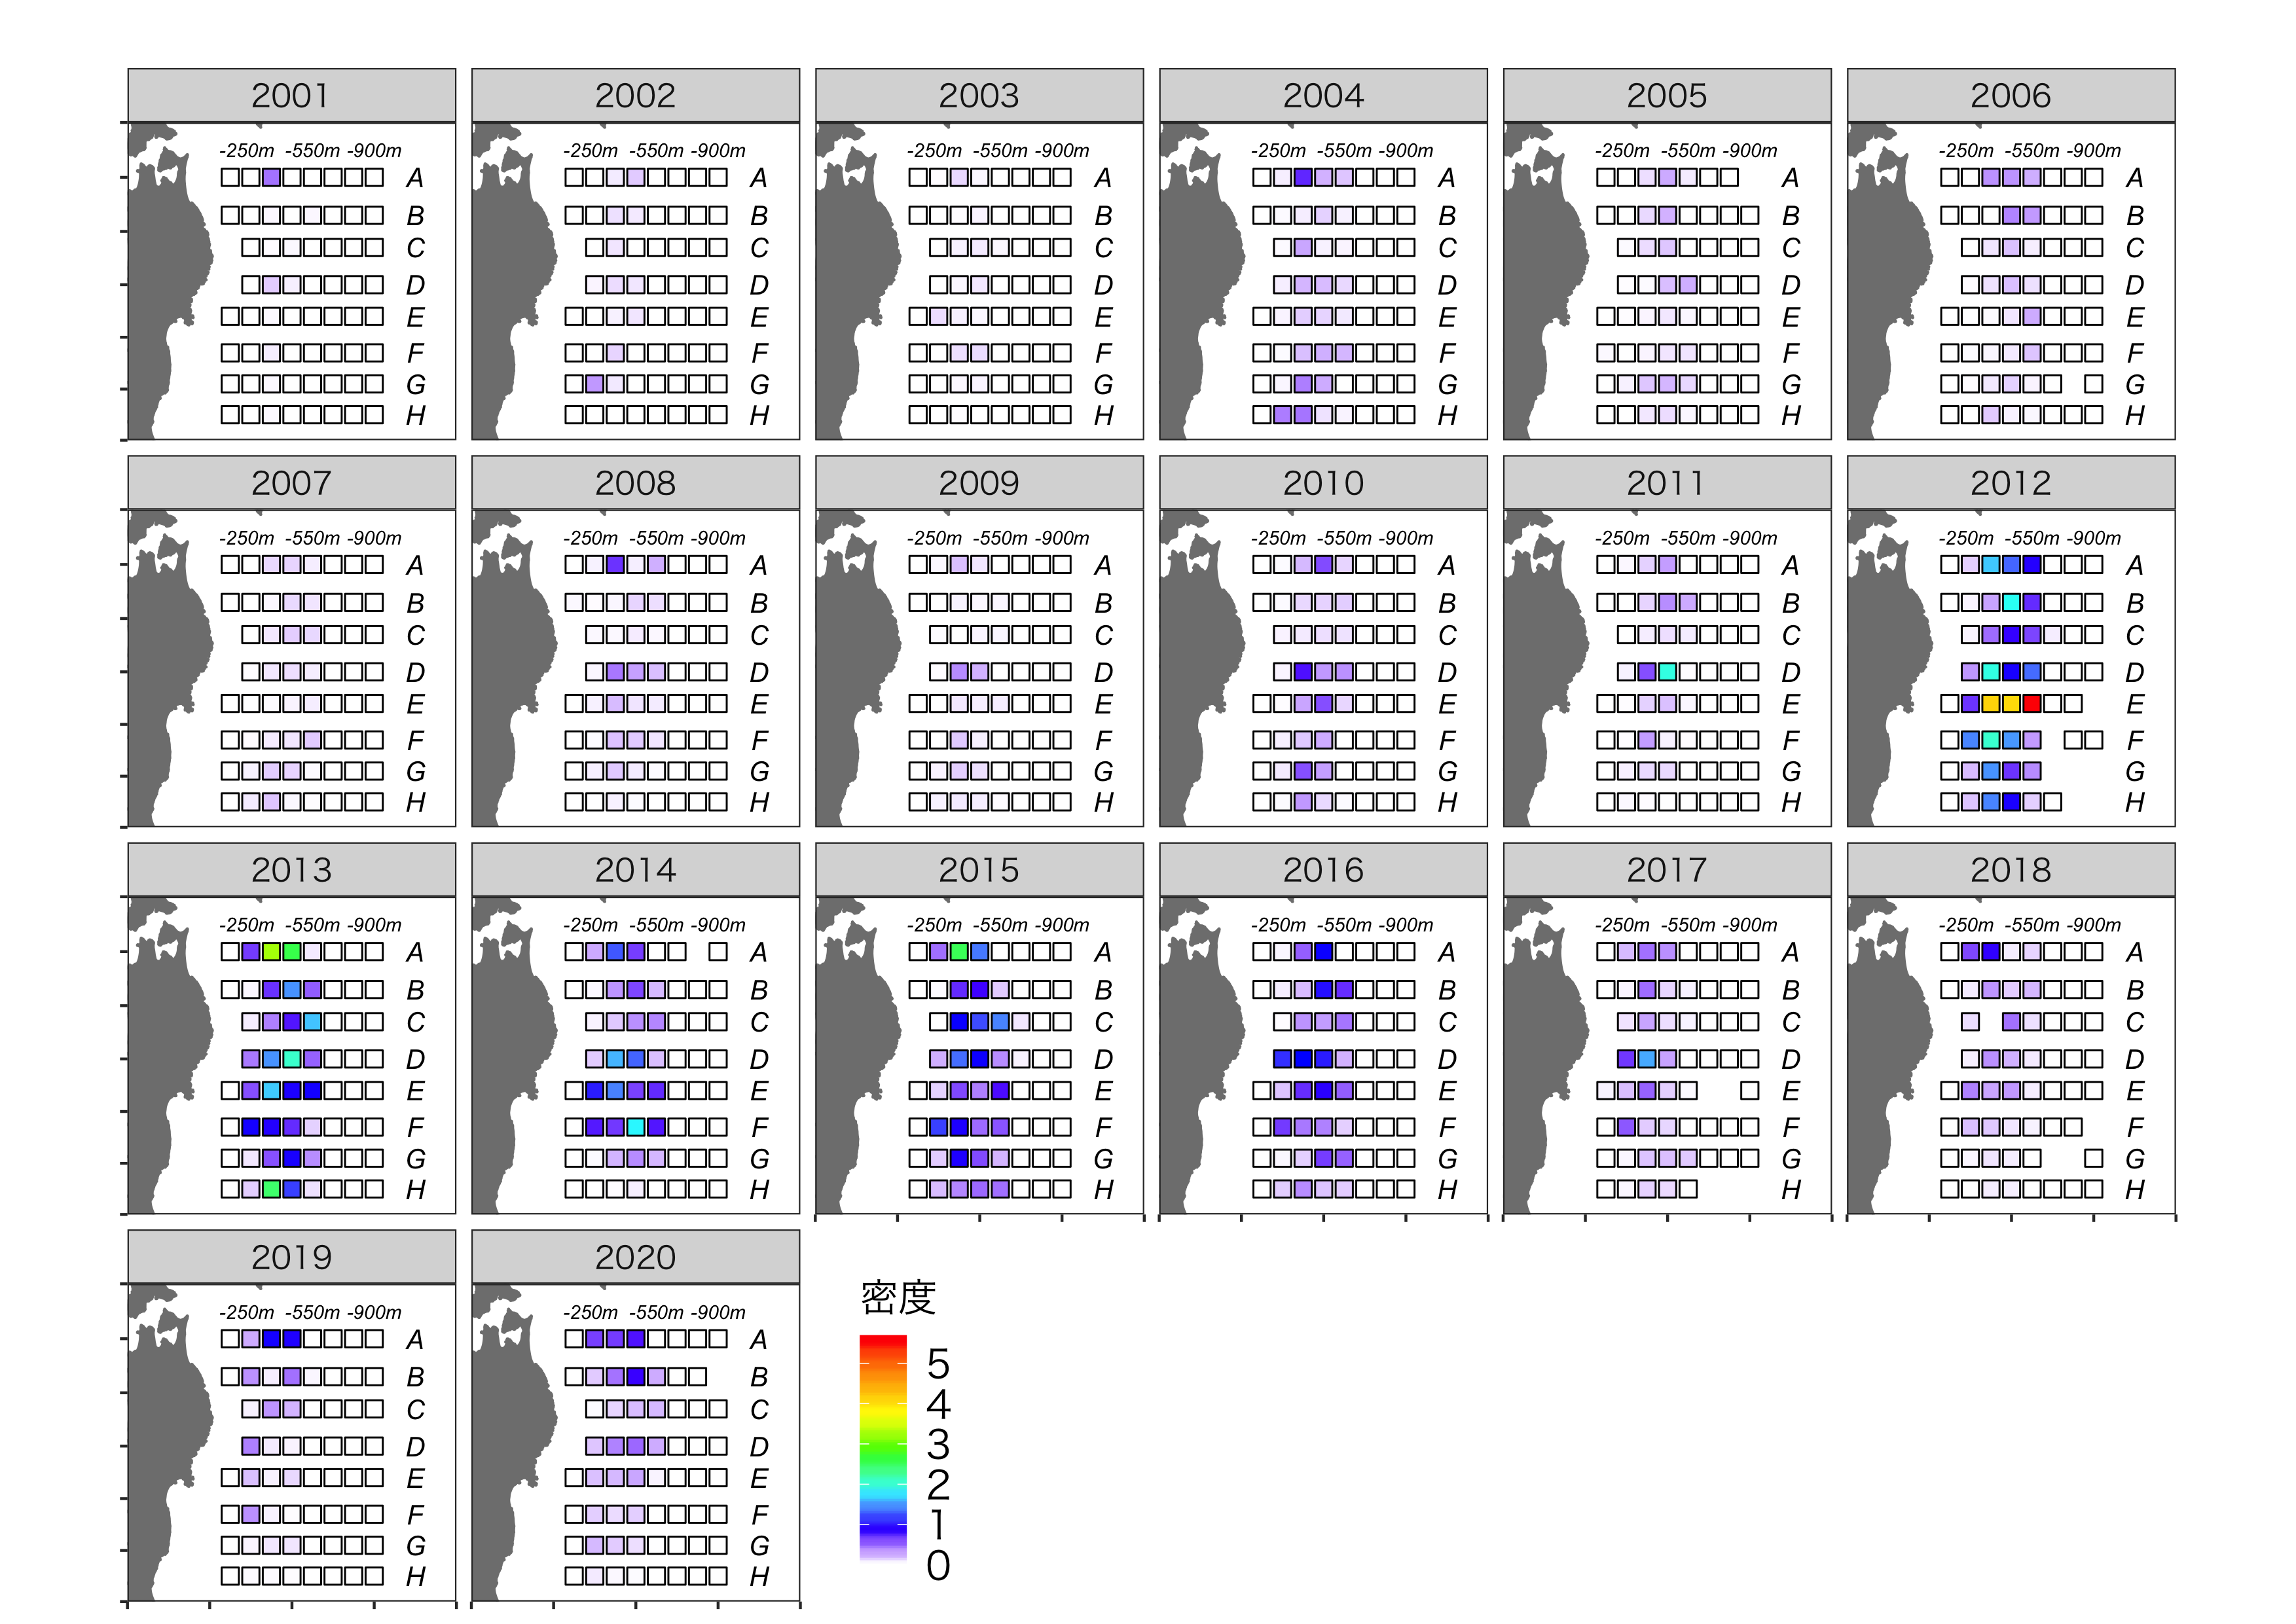
\includegraphics[width = 14cm]{マダラ2+dens.png}
  \caption{マダラ2歳魚以上の分布密度(千尾/km2)の経年変化}
\end{figure}

\begin{figure}[h]
  \centering
  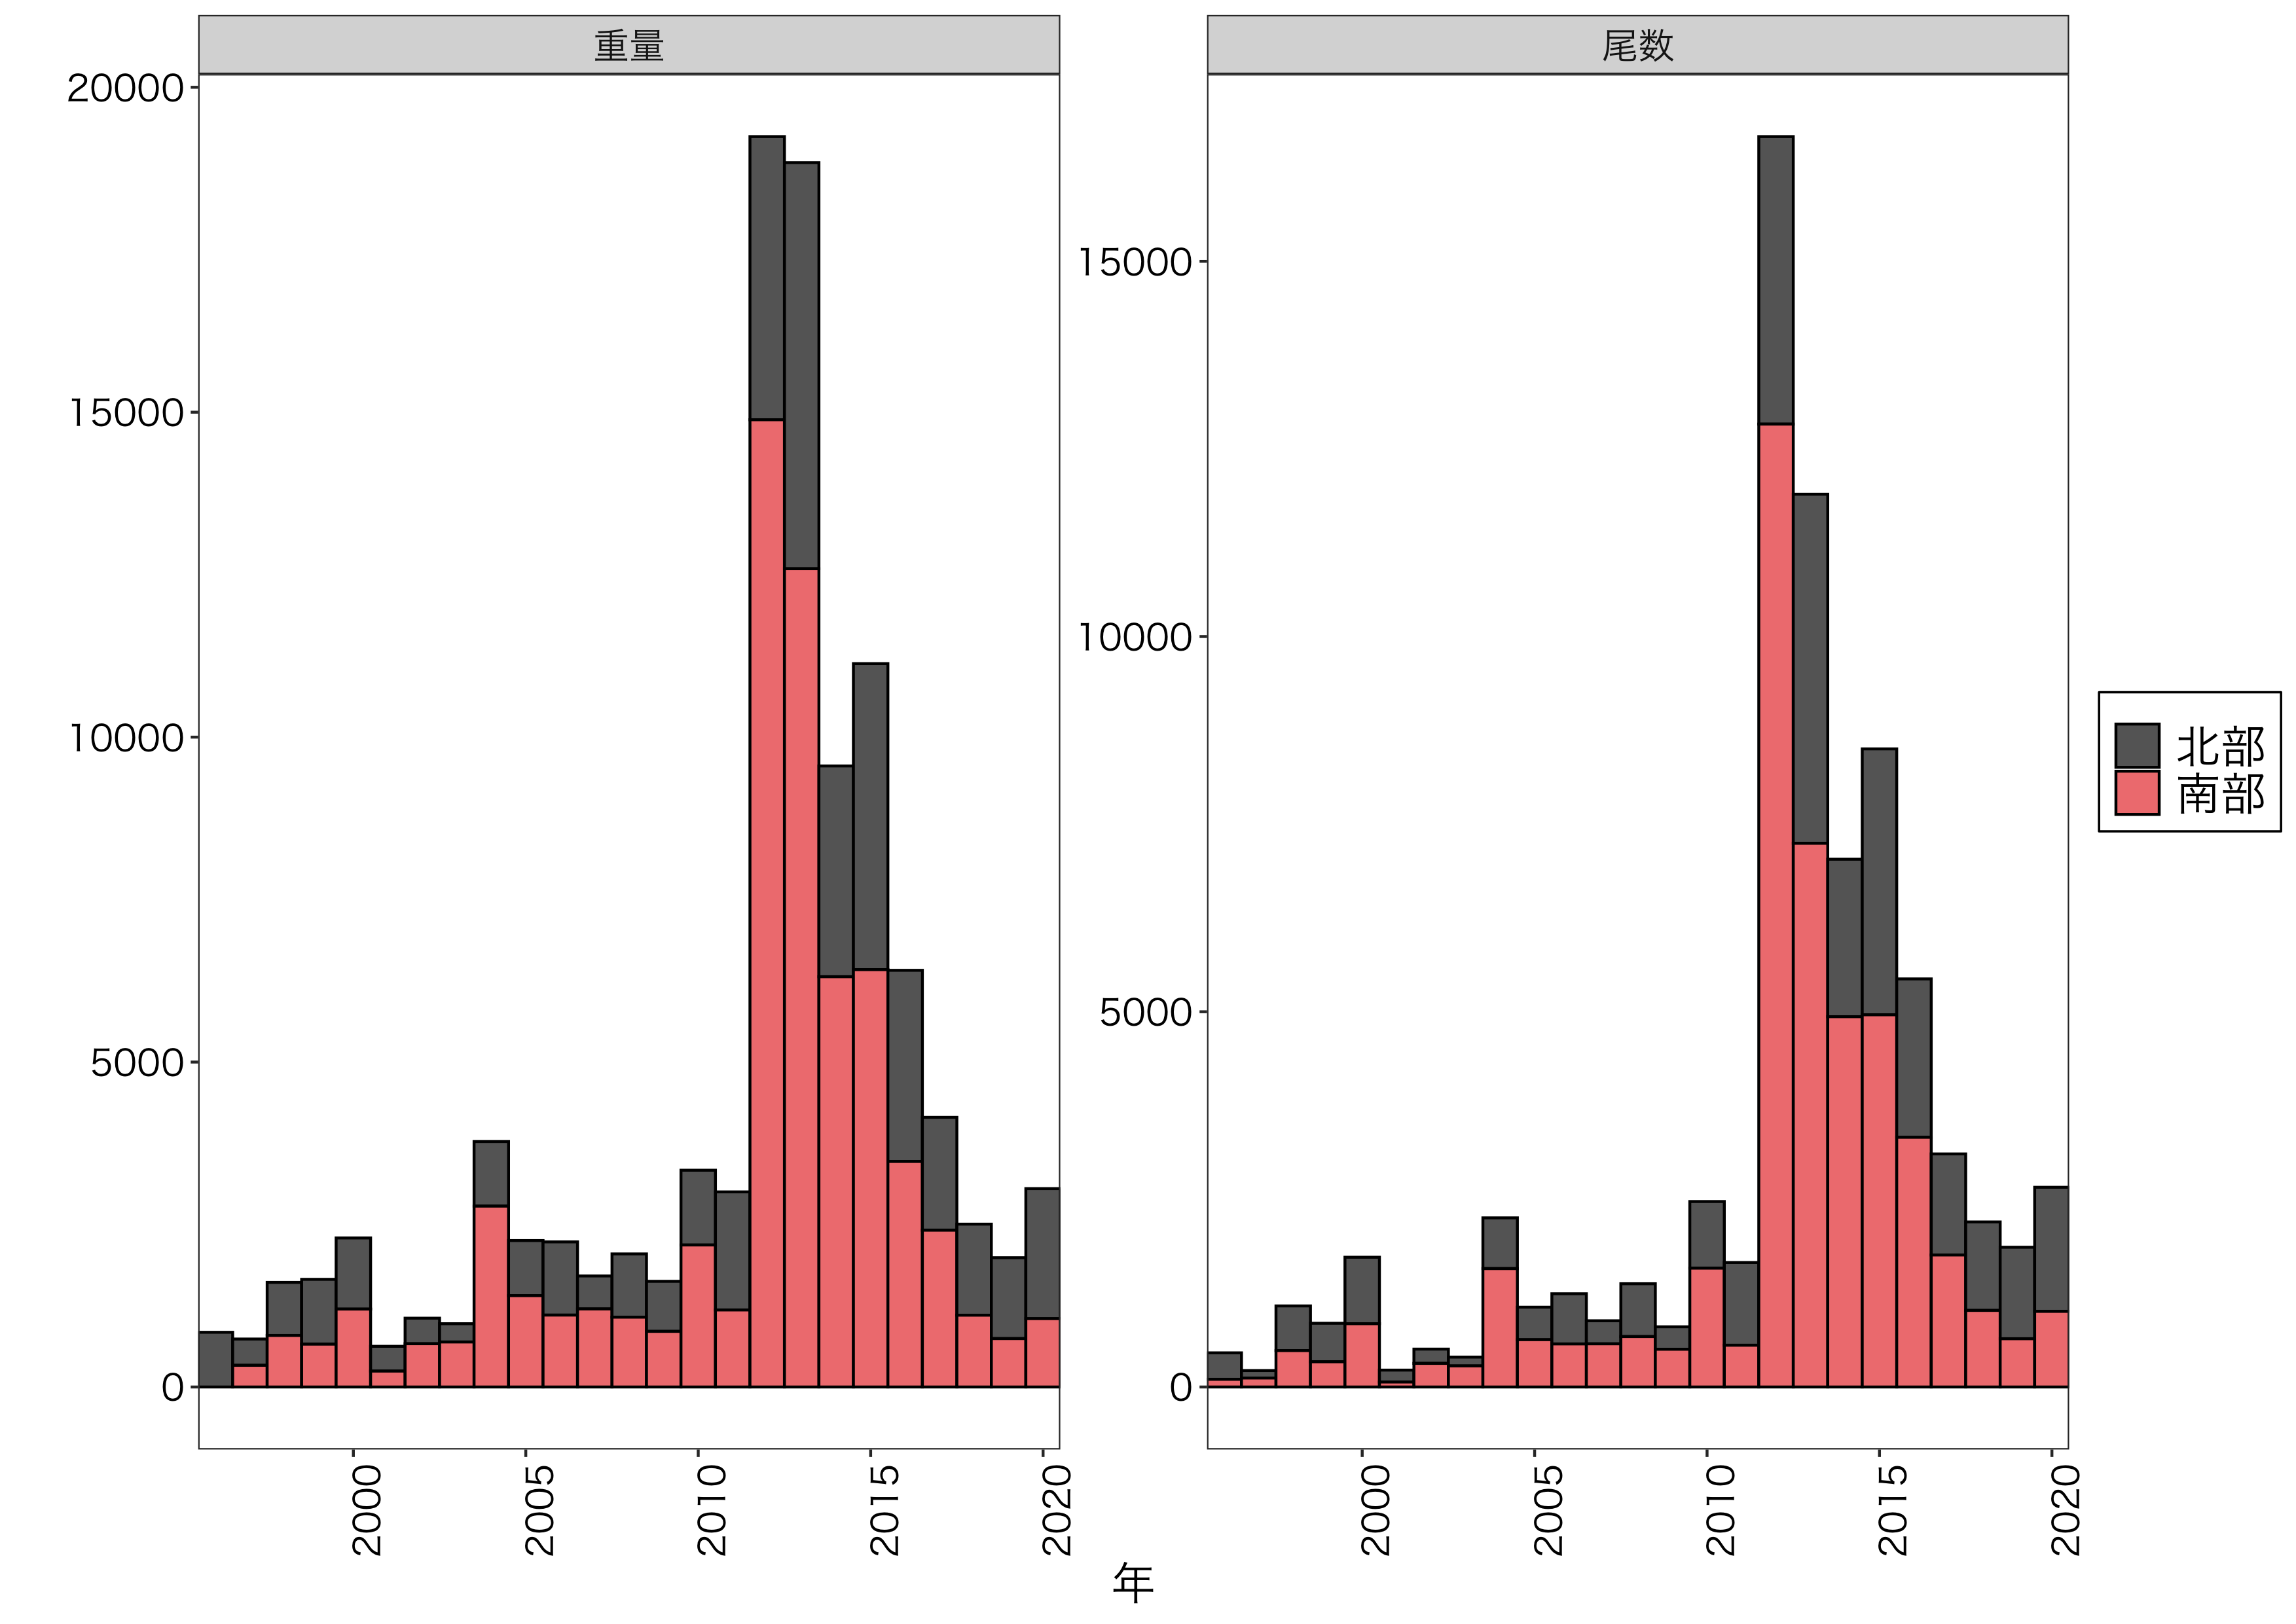
\includegraphics[width = 14cm]{マダラ2+trend.png}
  \caption{マダラ2歳魚以上の現存量(右; 単位は千トン)と現存尾数(左; 単位は百万尾)の経年変化}
\end{figure}

\begin{figure}[h]
  \centering
  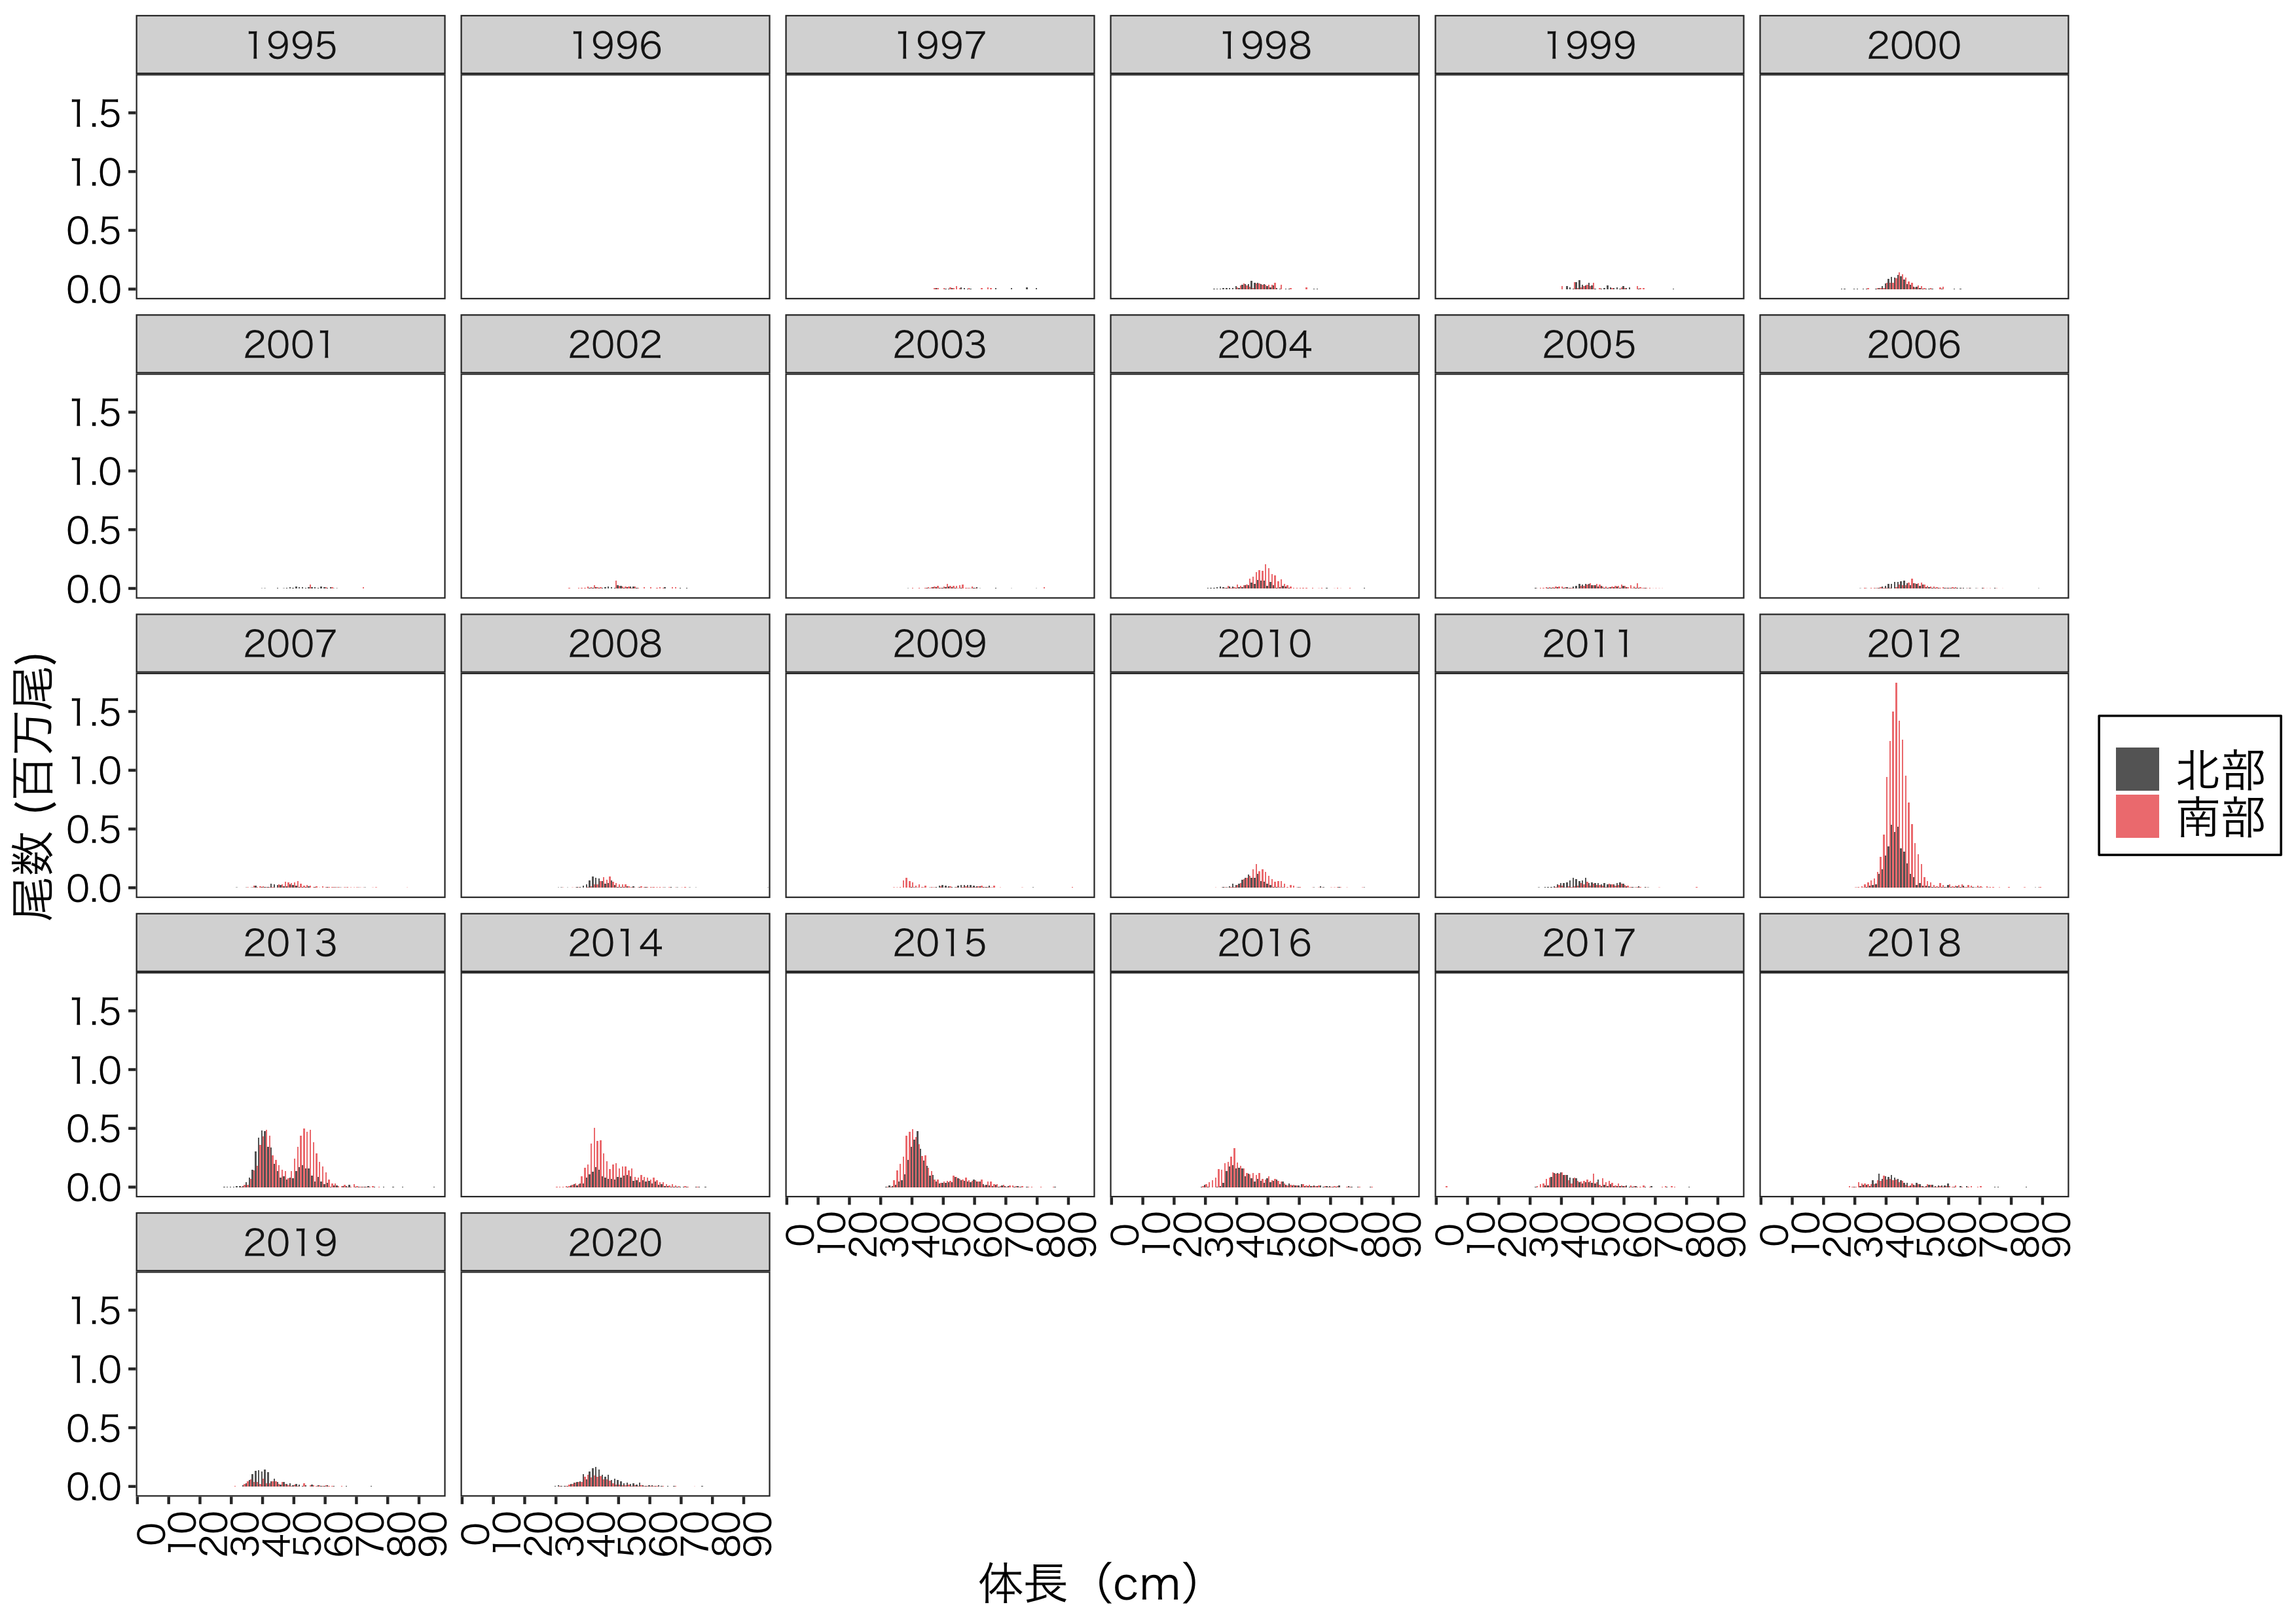
\includegraphics[width = 14cm]{マダラ2+length.png}
  \caption{マダラ2歳魚以上の体長組成の経年変化}
\end{figure}

\begin{figure}[h]
  \centering
  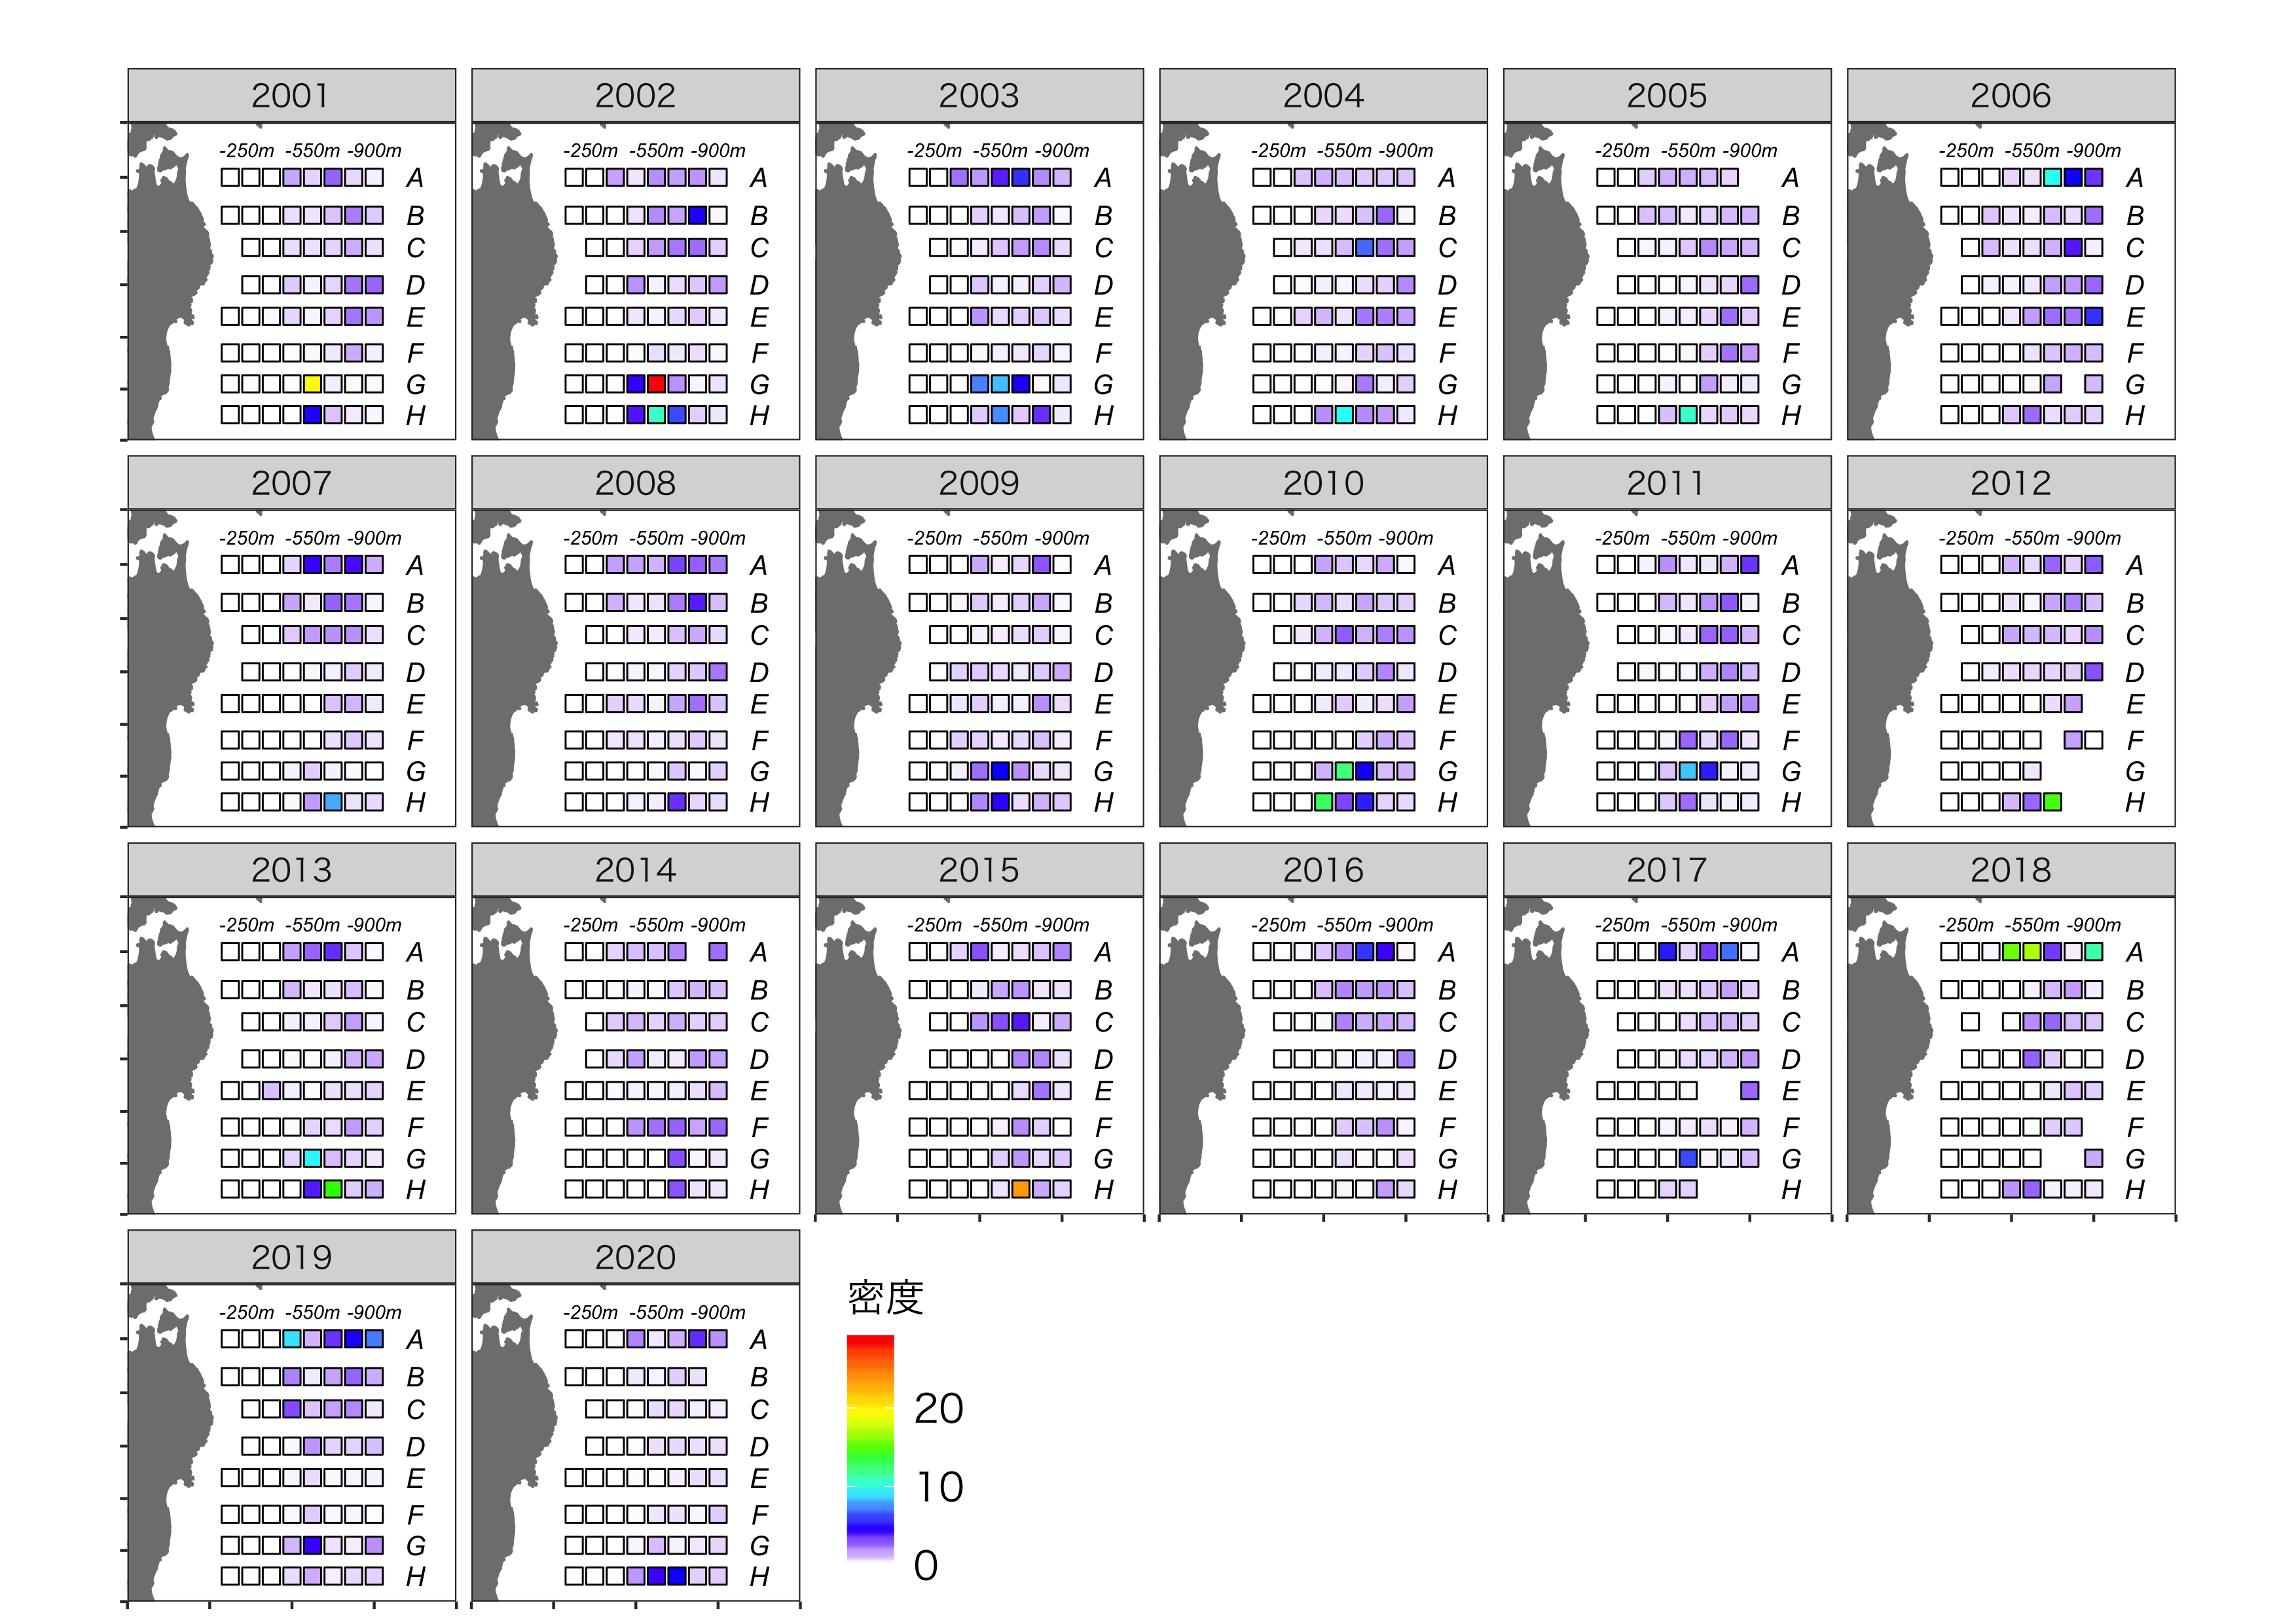
\includegraphics[width = 14cm]{イトヒキダラdens.png}
  \caption{イトヒキダラの分布密度(千尾/km2)の経年変化}
\end{figure}

\begin{figure}[h]
  \centering
  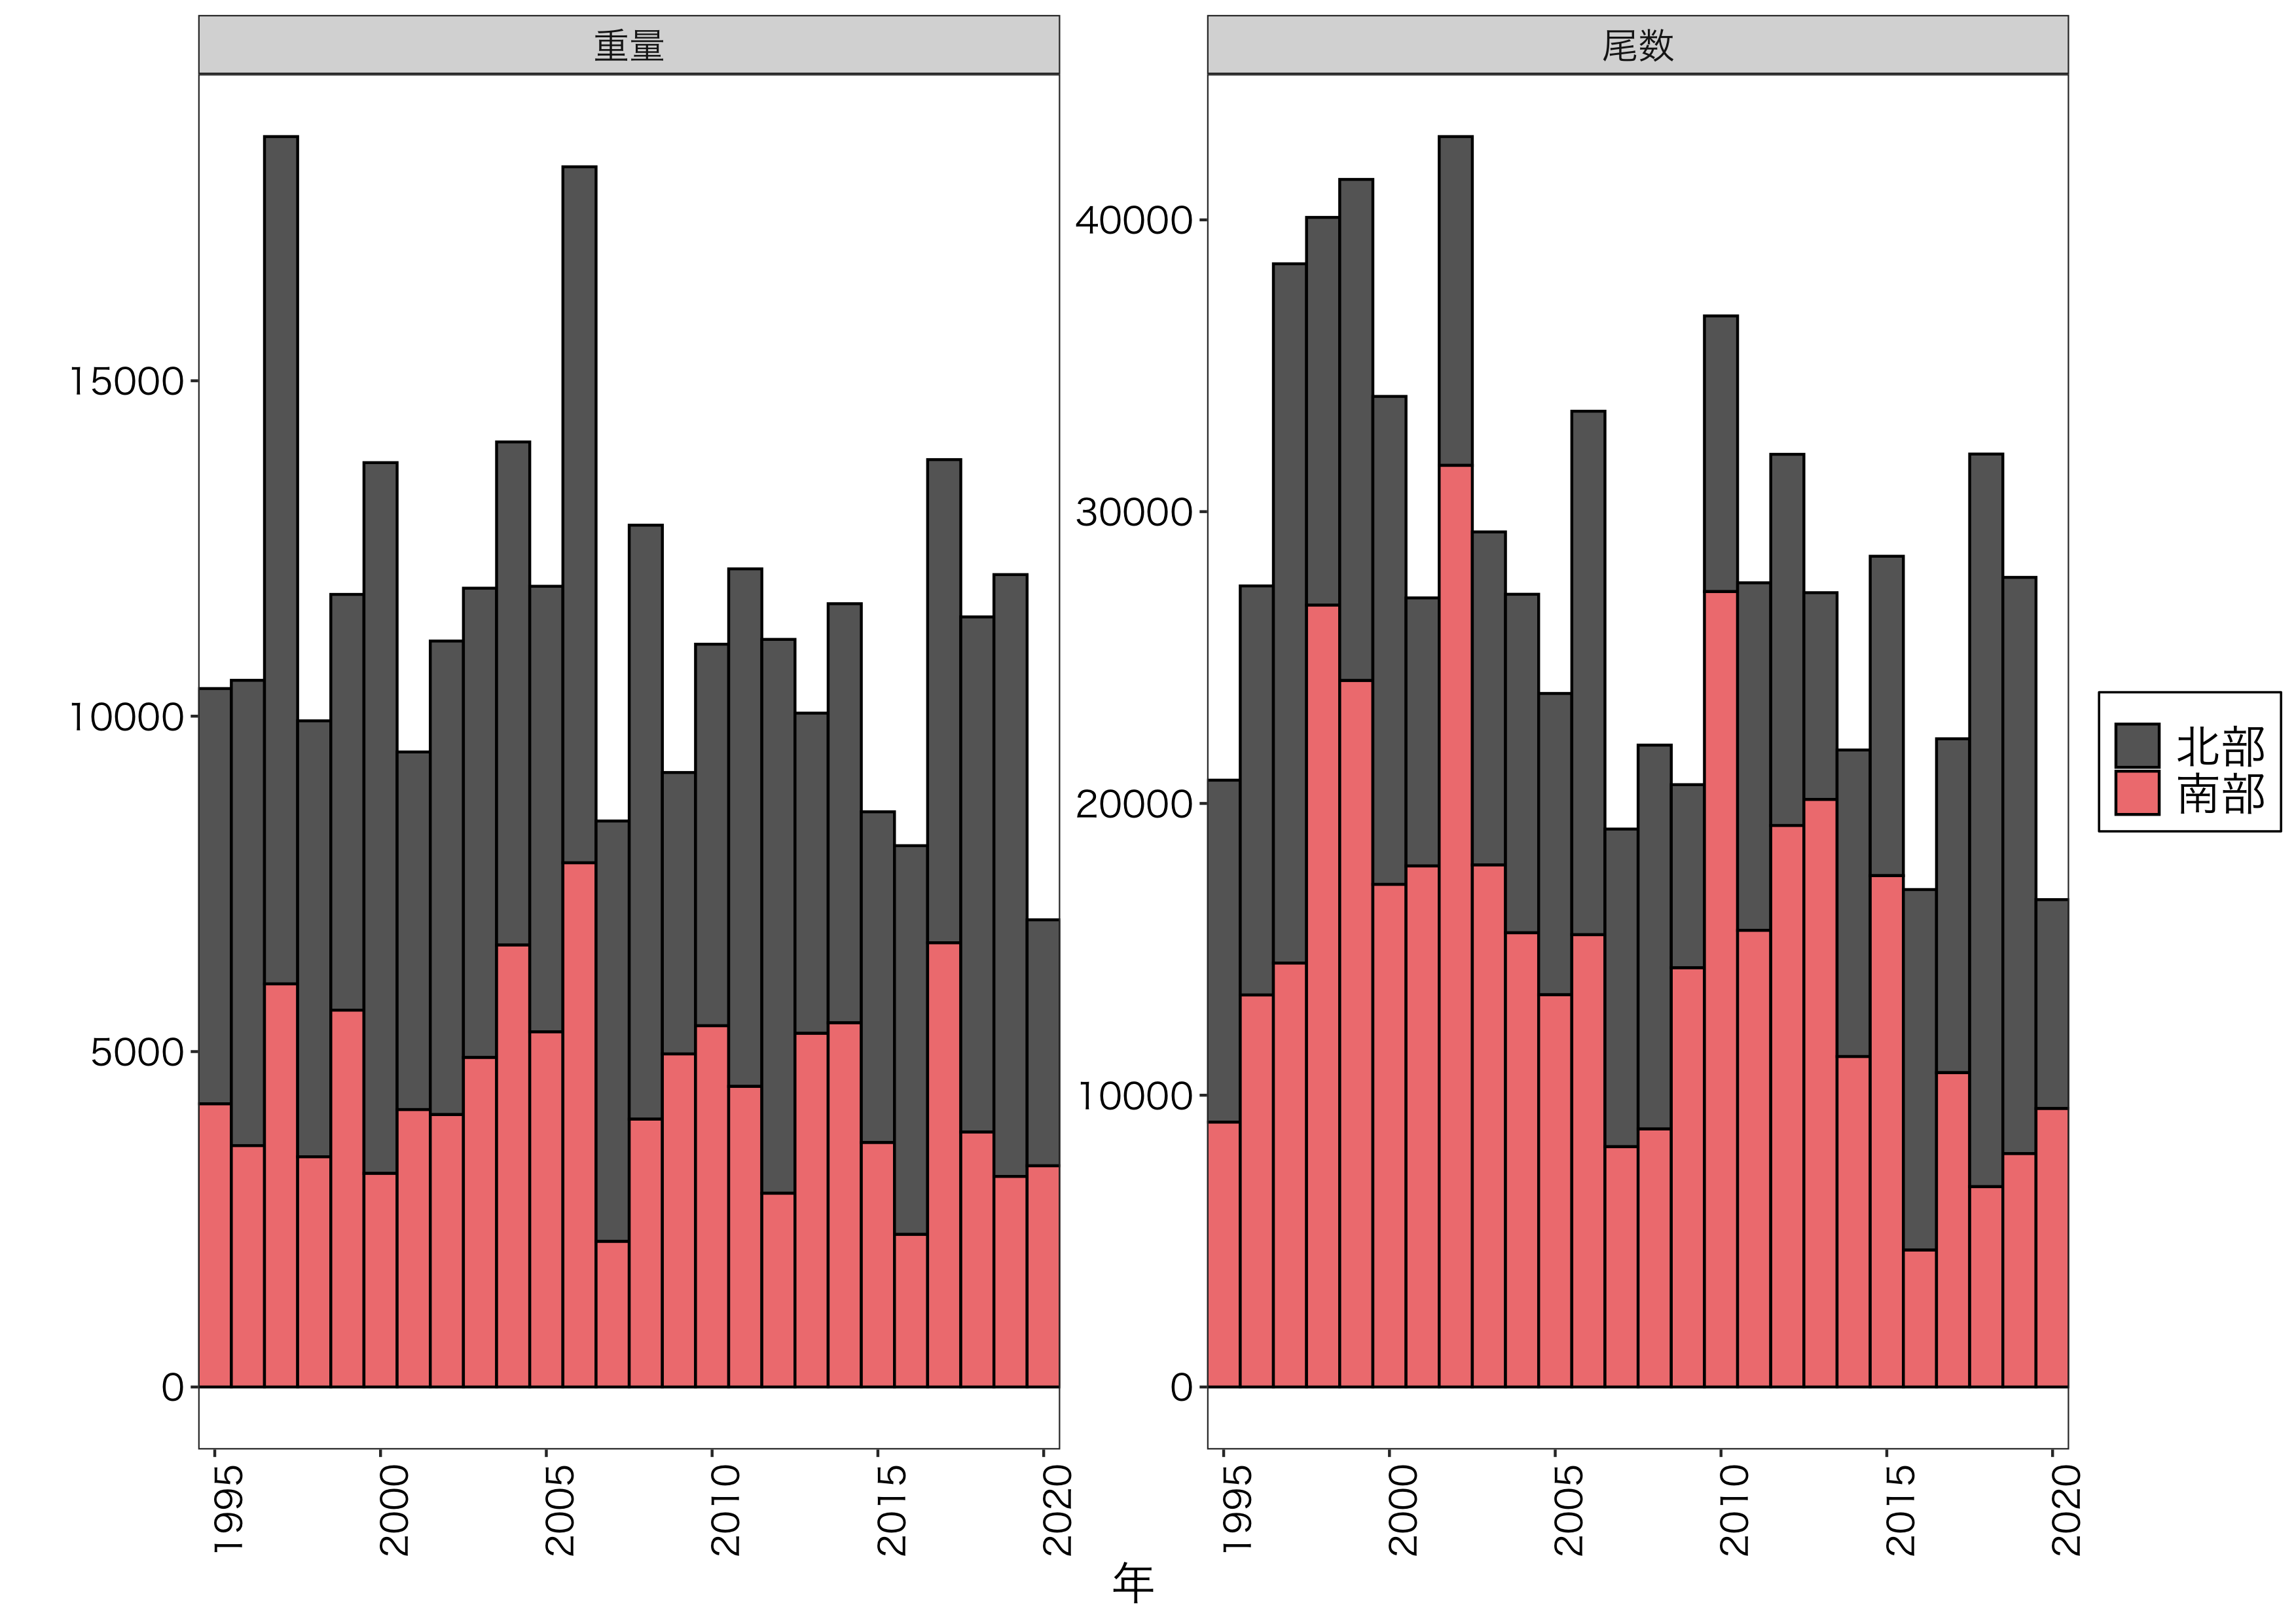
\includegraphics[width = 14cm]{イトヒキダラtrend.png}
  \caption{イトヒキダラの現存量(右; 単位は千トン)と現存尾数(左; 単位は百万尾)の経年変化}
\end{figure}

\begin{figure}[h]
  \centering
  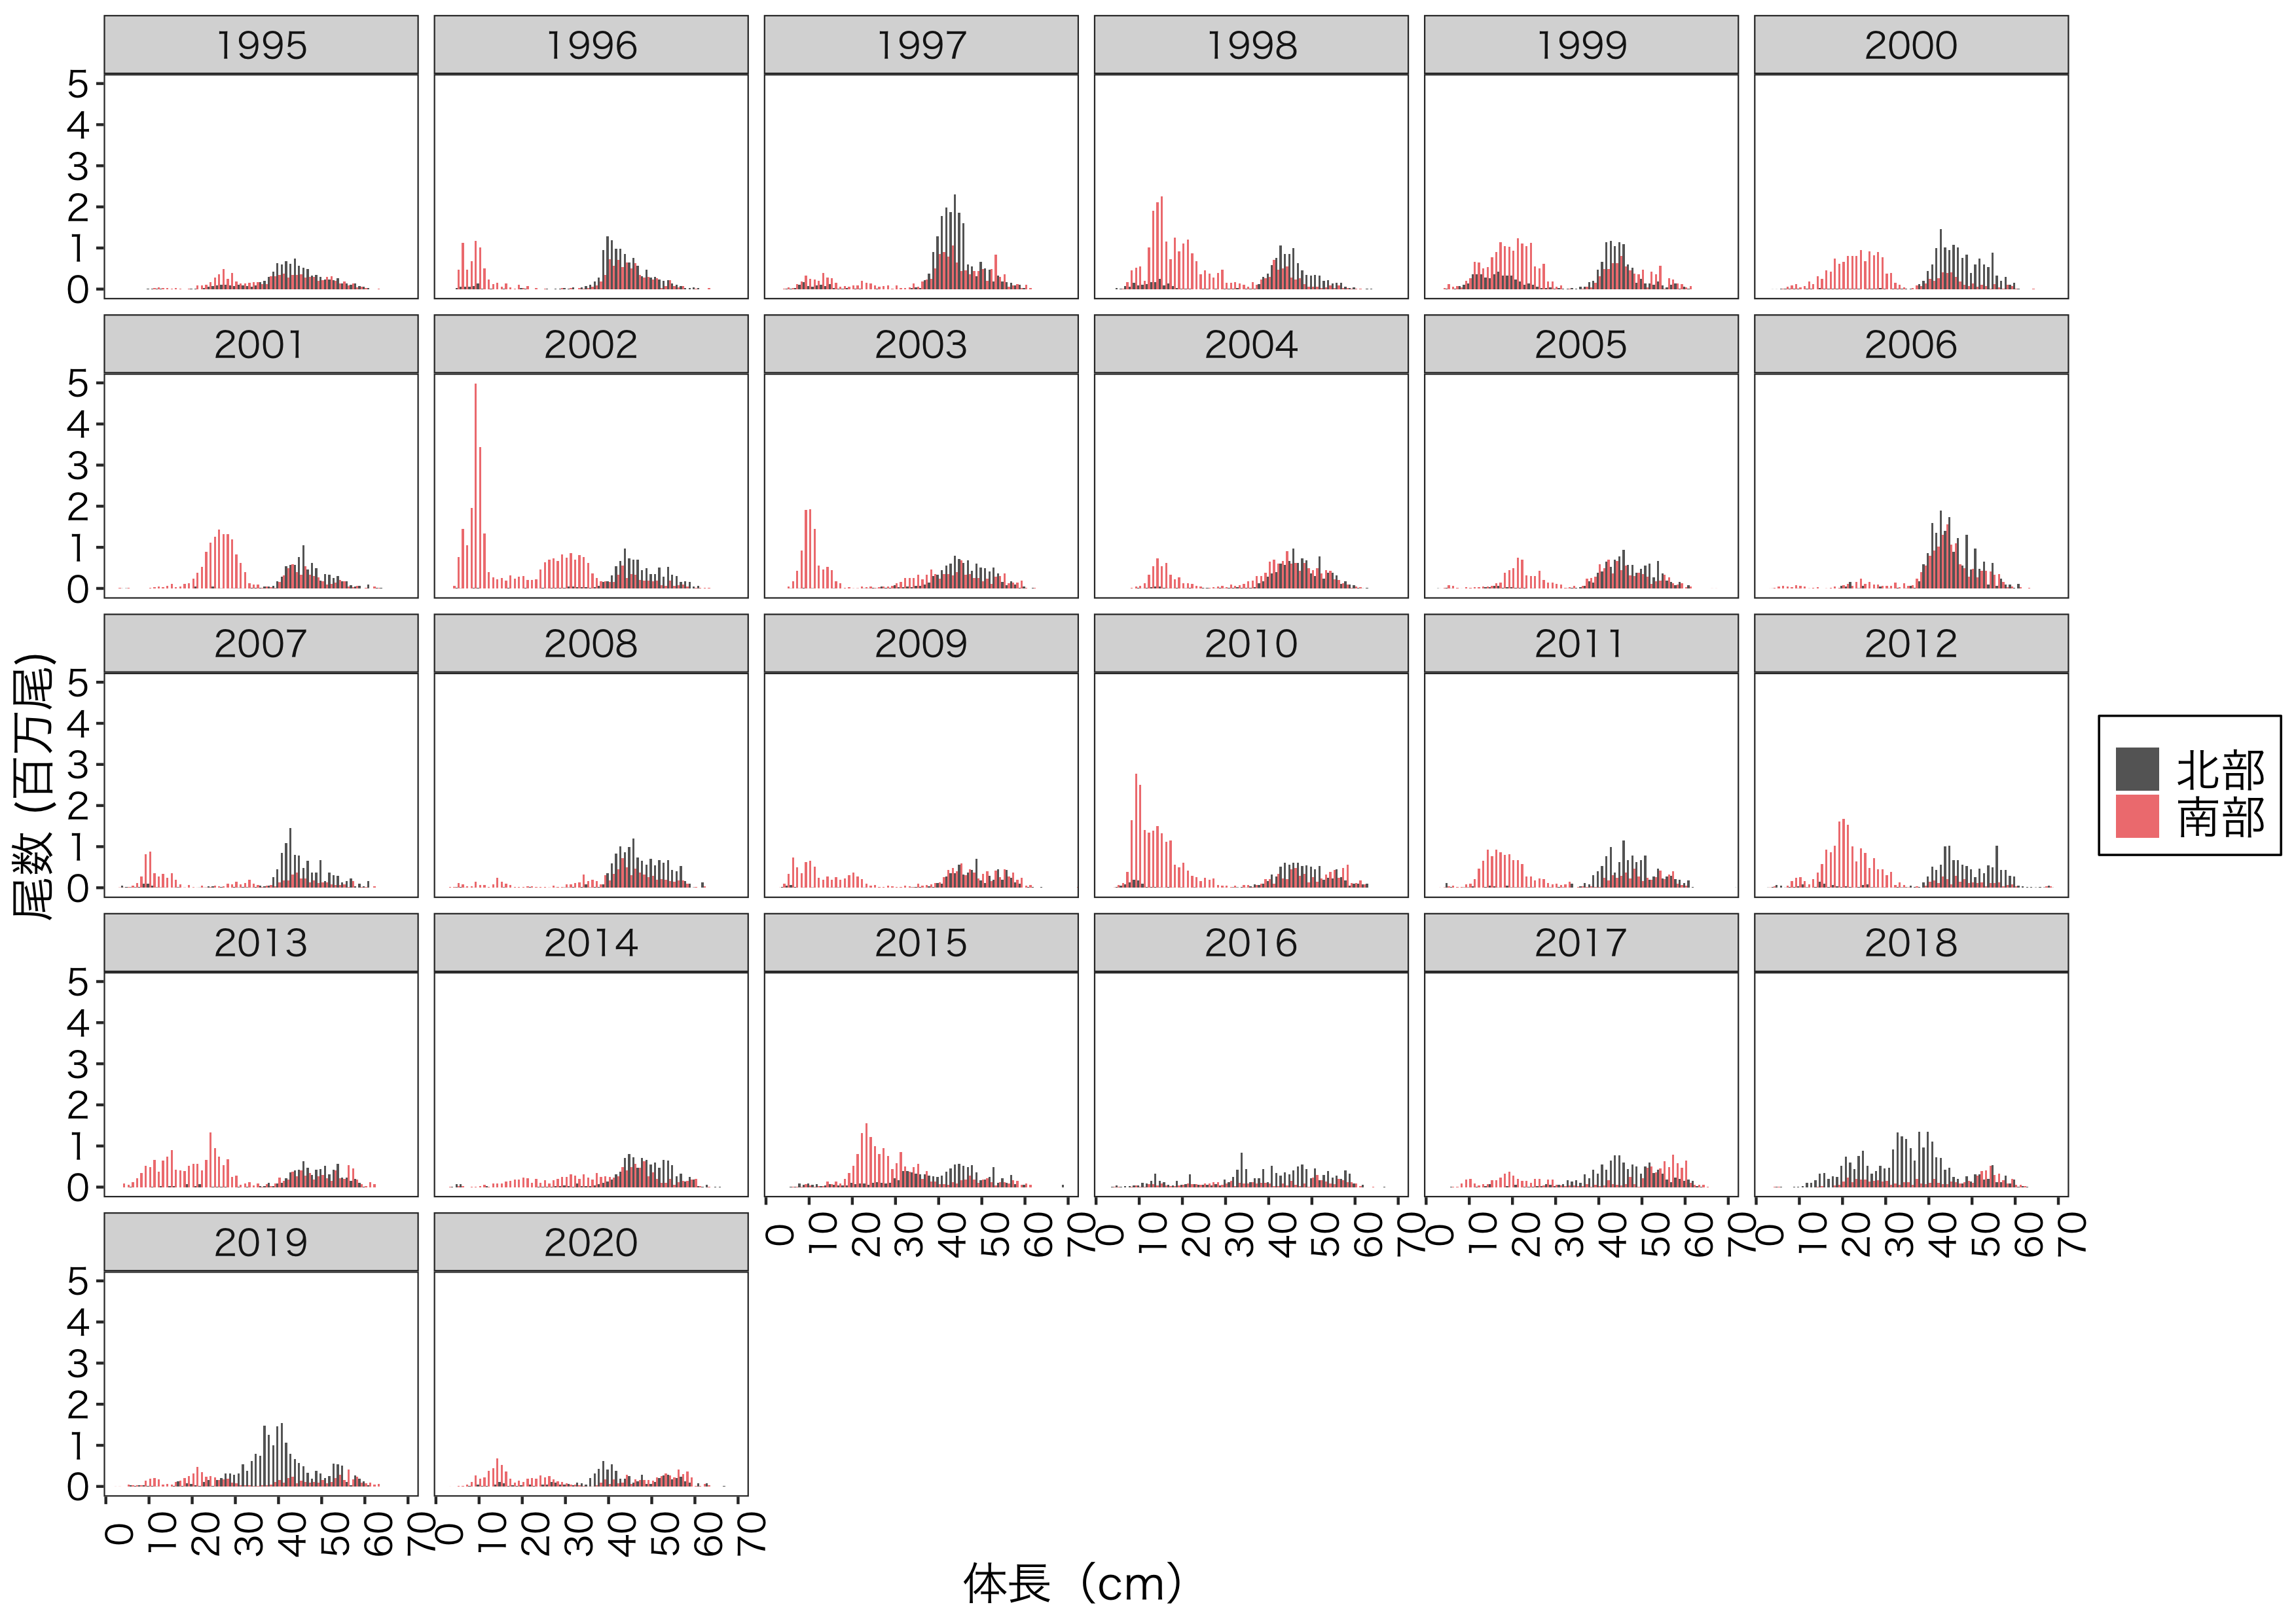
\includegraphics[width = 14cm]{イトヒキダラlength.png}
  \caption{イトヒキダラの体長組成の経年変化}
\end{figure}

\begin{figure}[h]
  \centering
  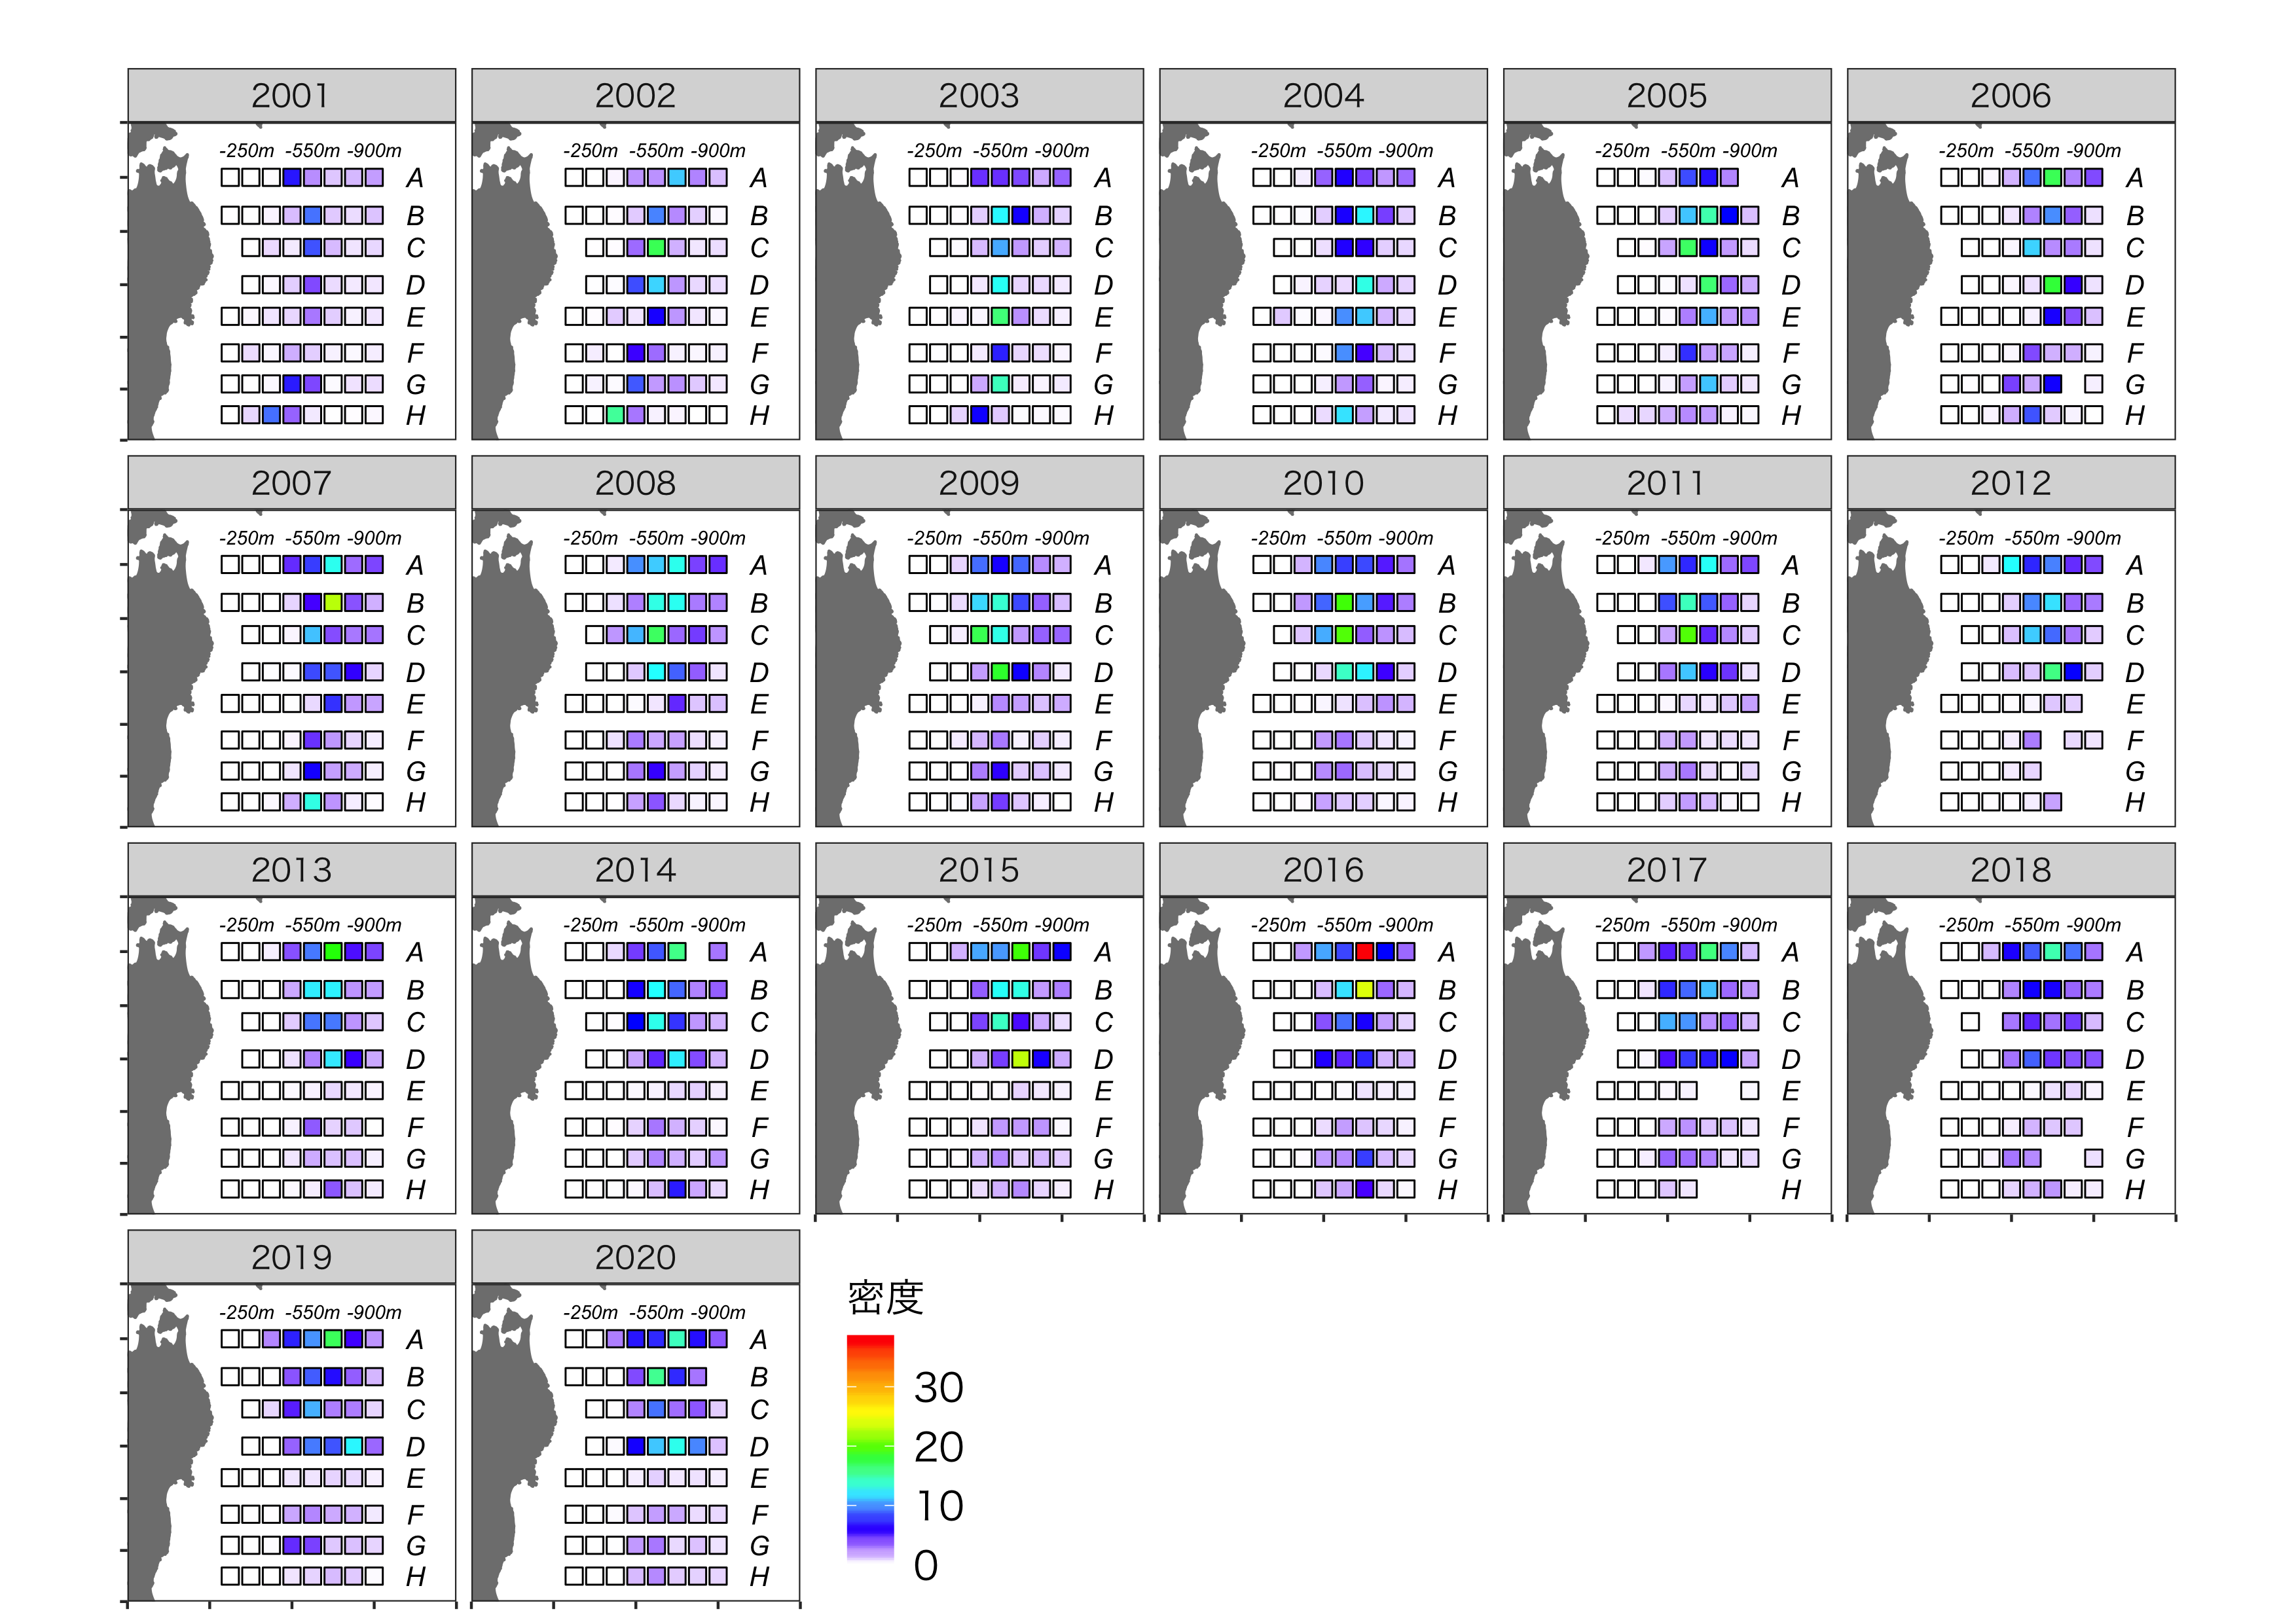
\includegraphics[width = 14cm]{キチジdens.png}
  \caption{キチジの分布密度(千尾/km2)の経年変化}
\end{figure}

\begin{figure}[h]
  \centering
  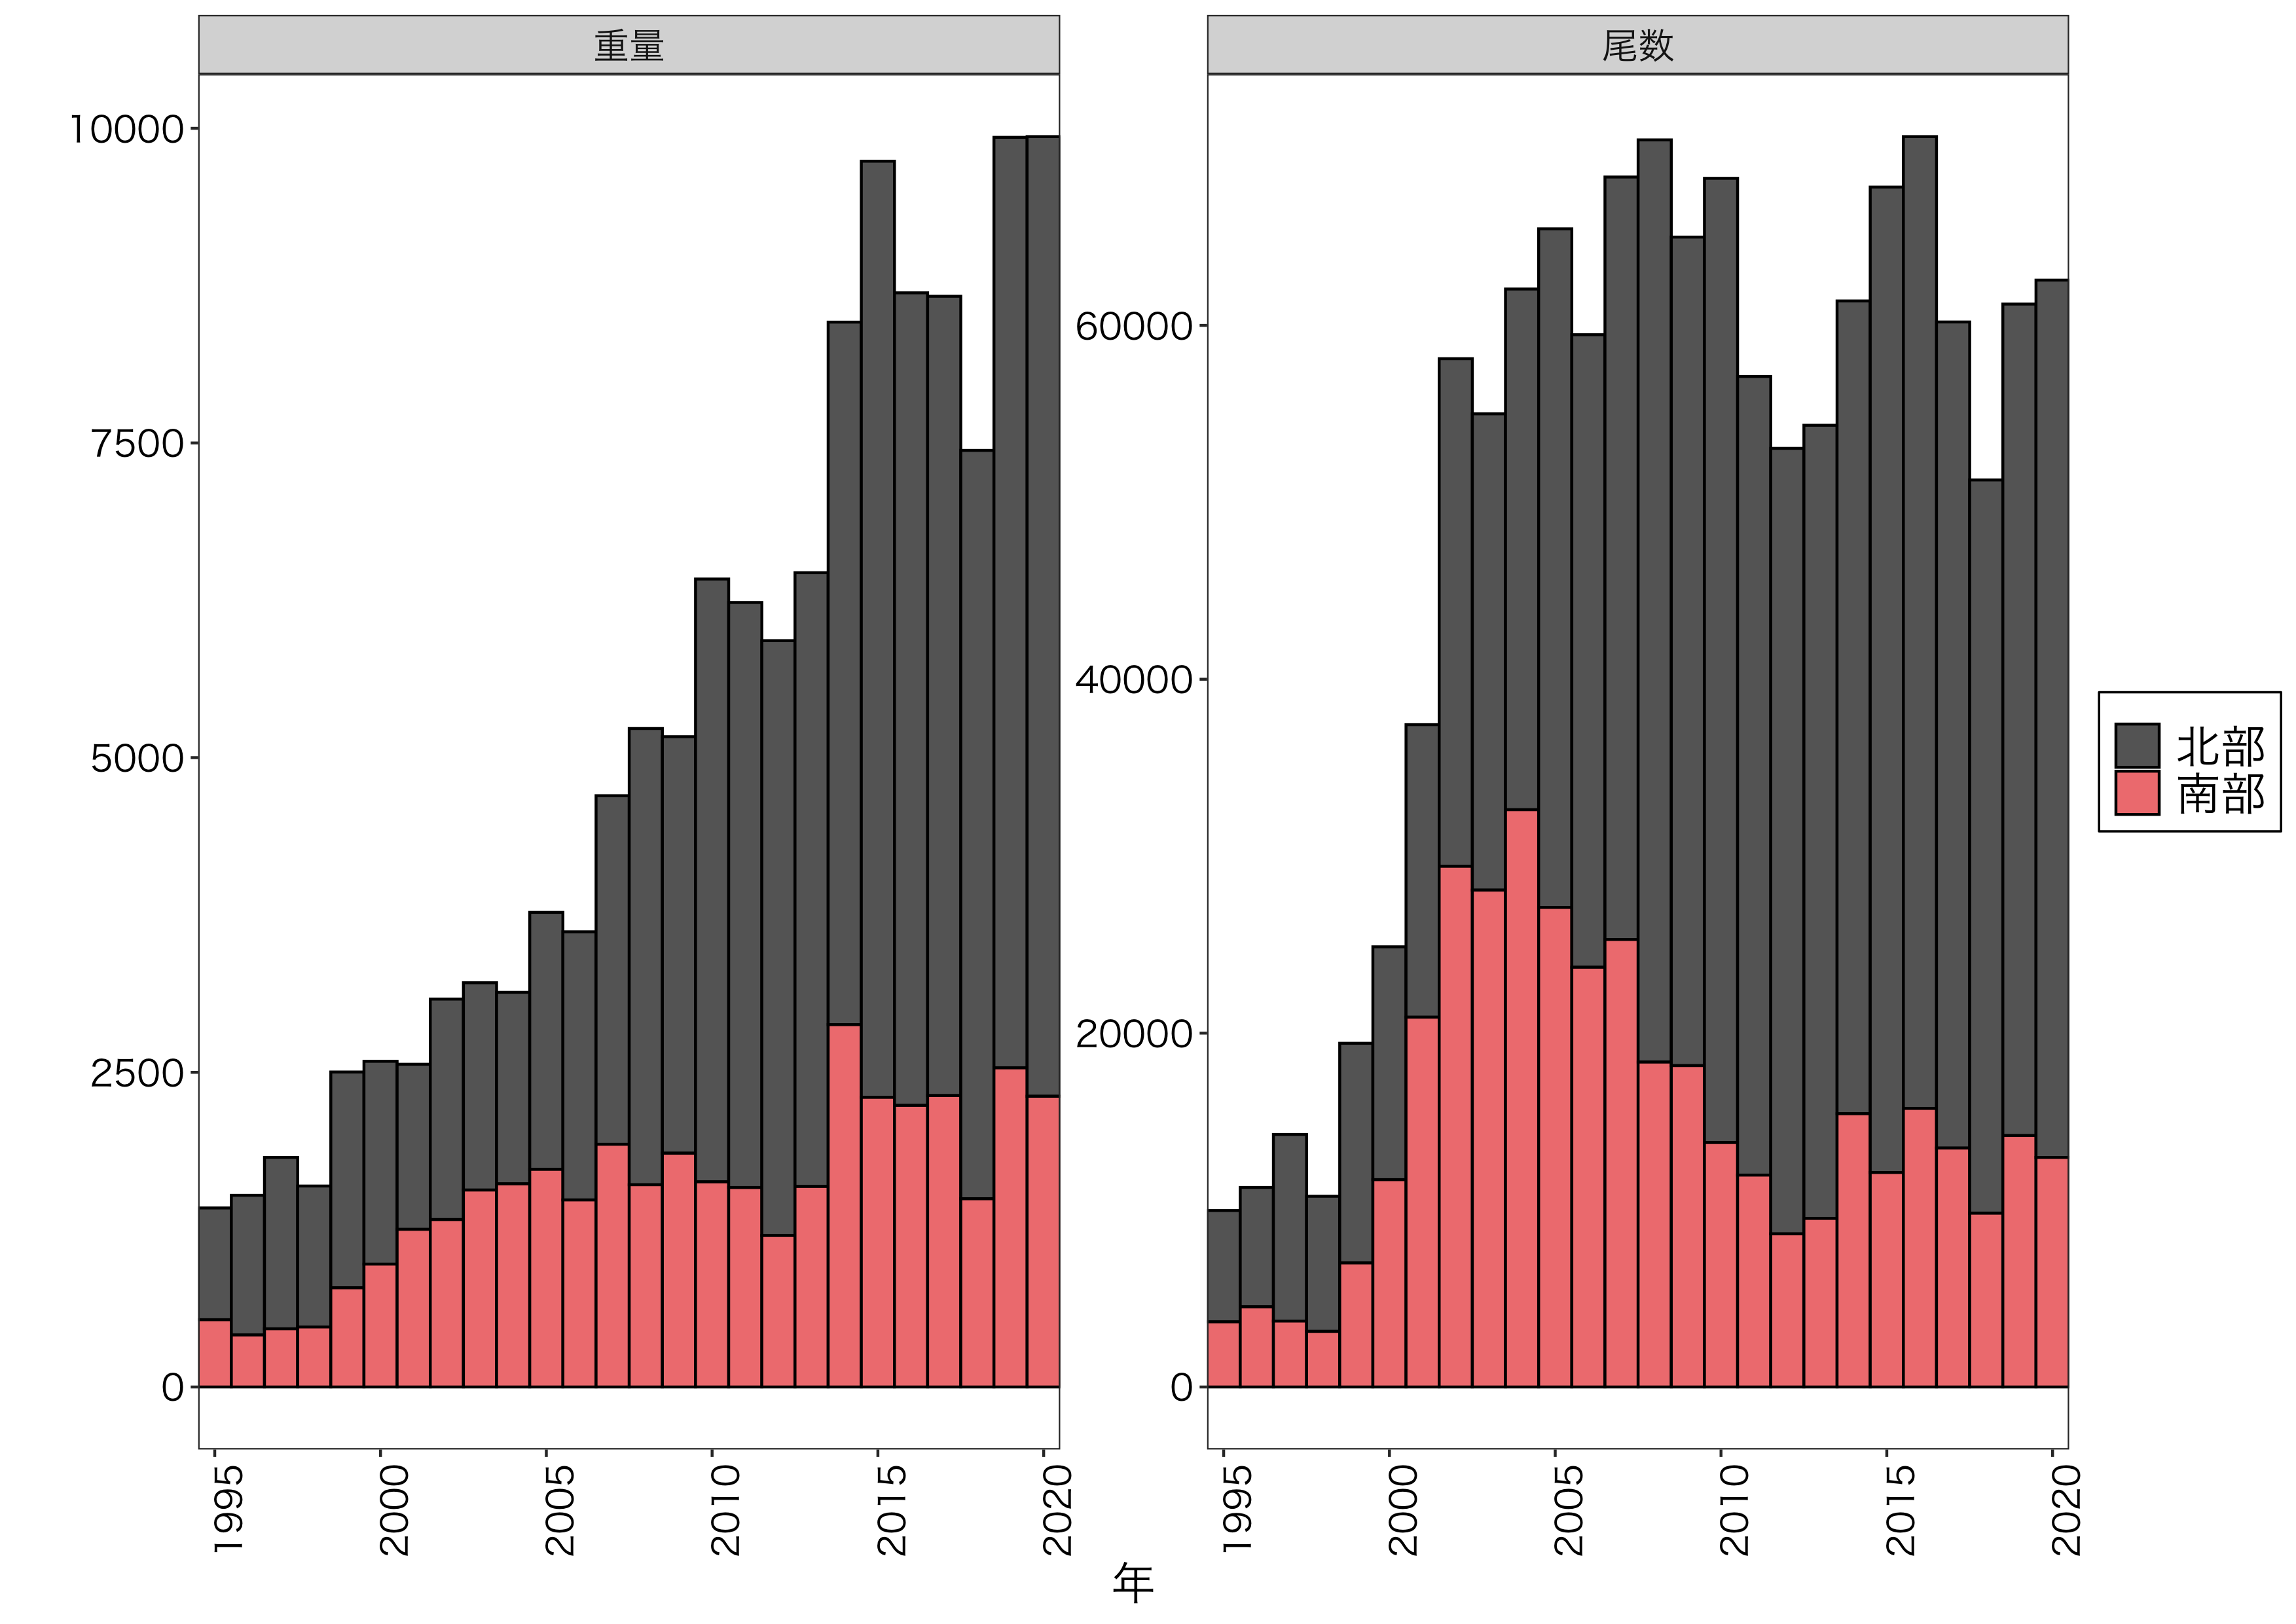
\includegraphics[width = 14cm]{キチジtrend.png}
  \caption{キチジの現存量(右; 単位は千トン)と現存尾数(左; 単位は百万尾)の経年変化}
\end{figure}

\begin{figure}[h]
  \centering
  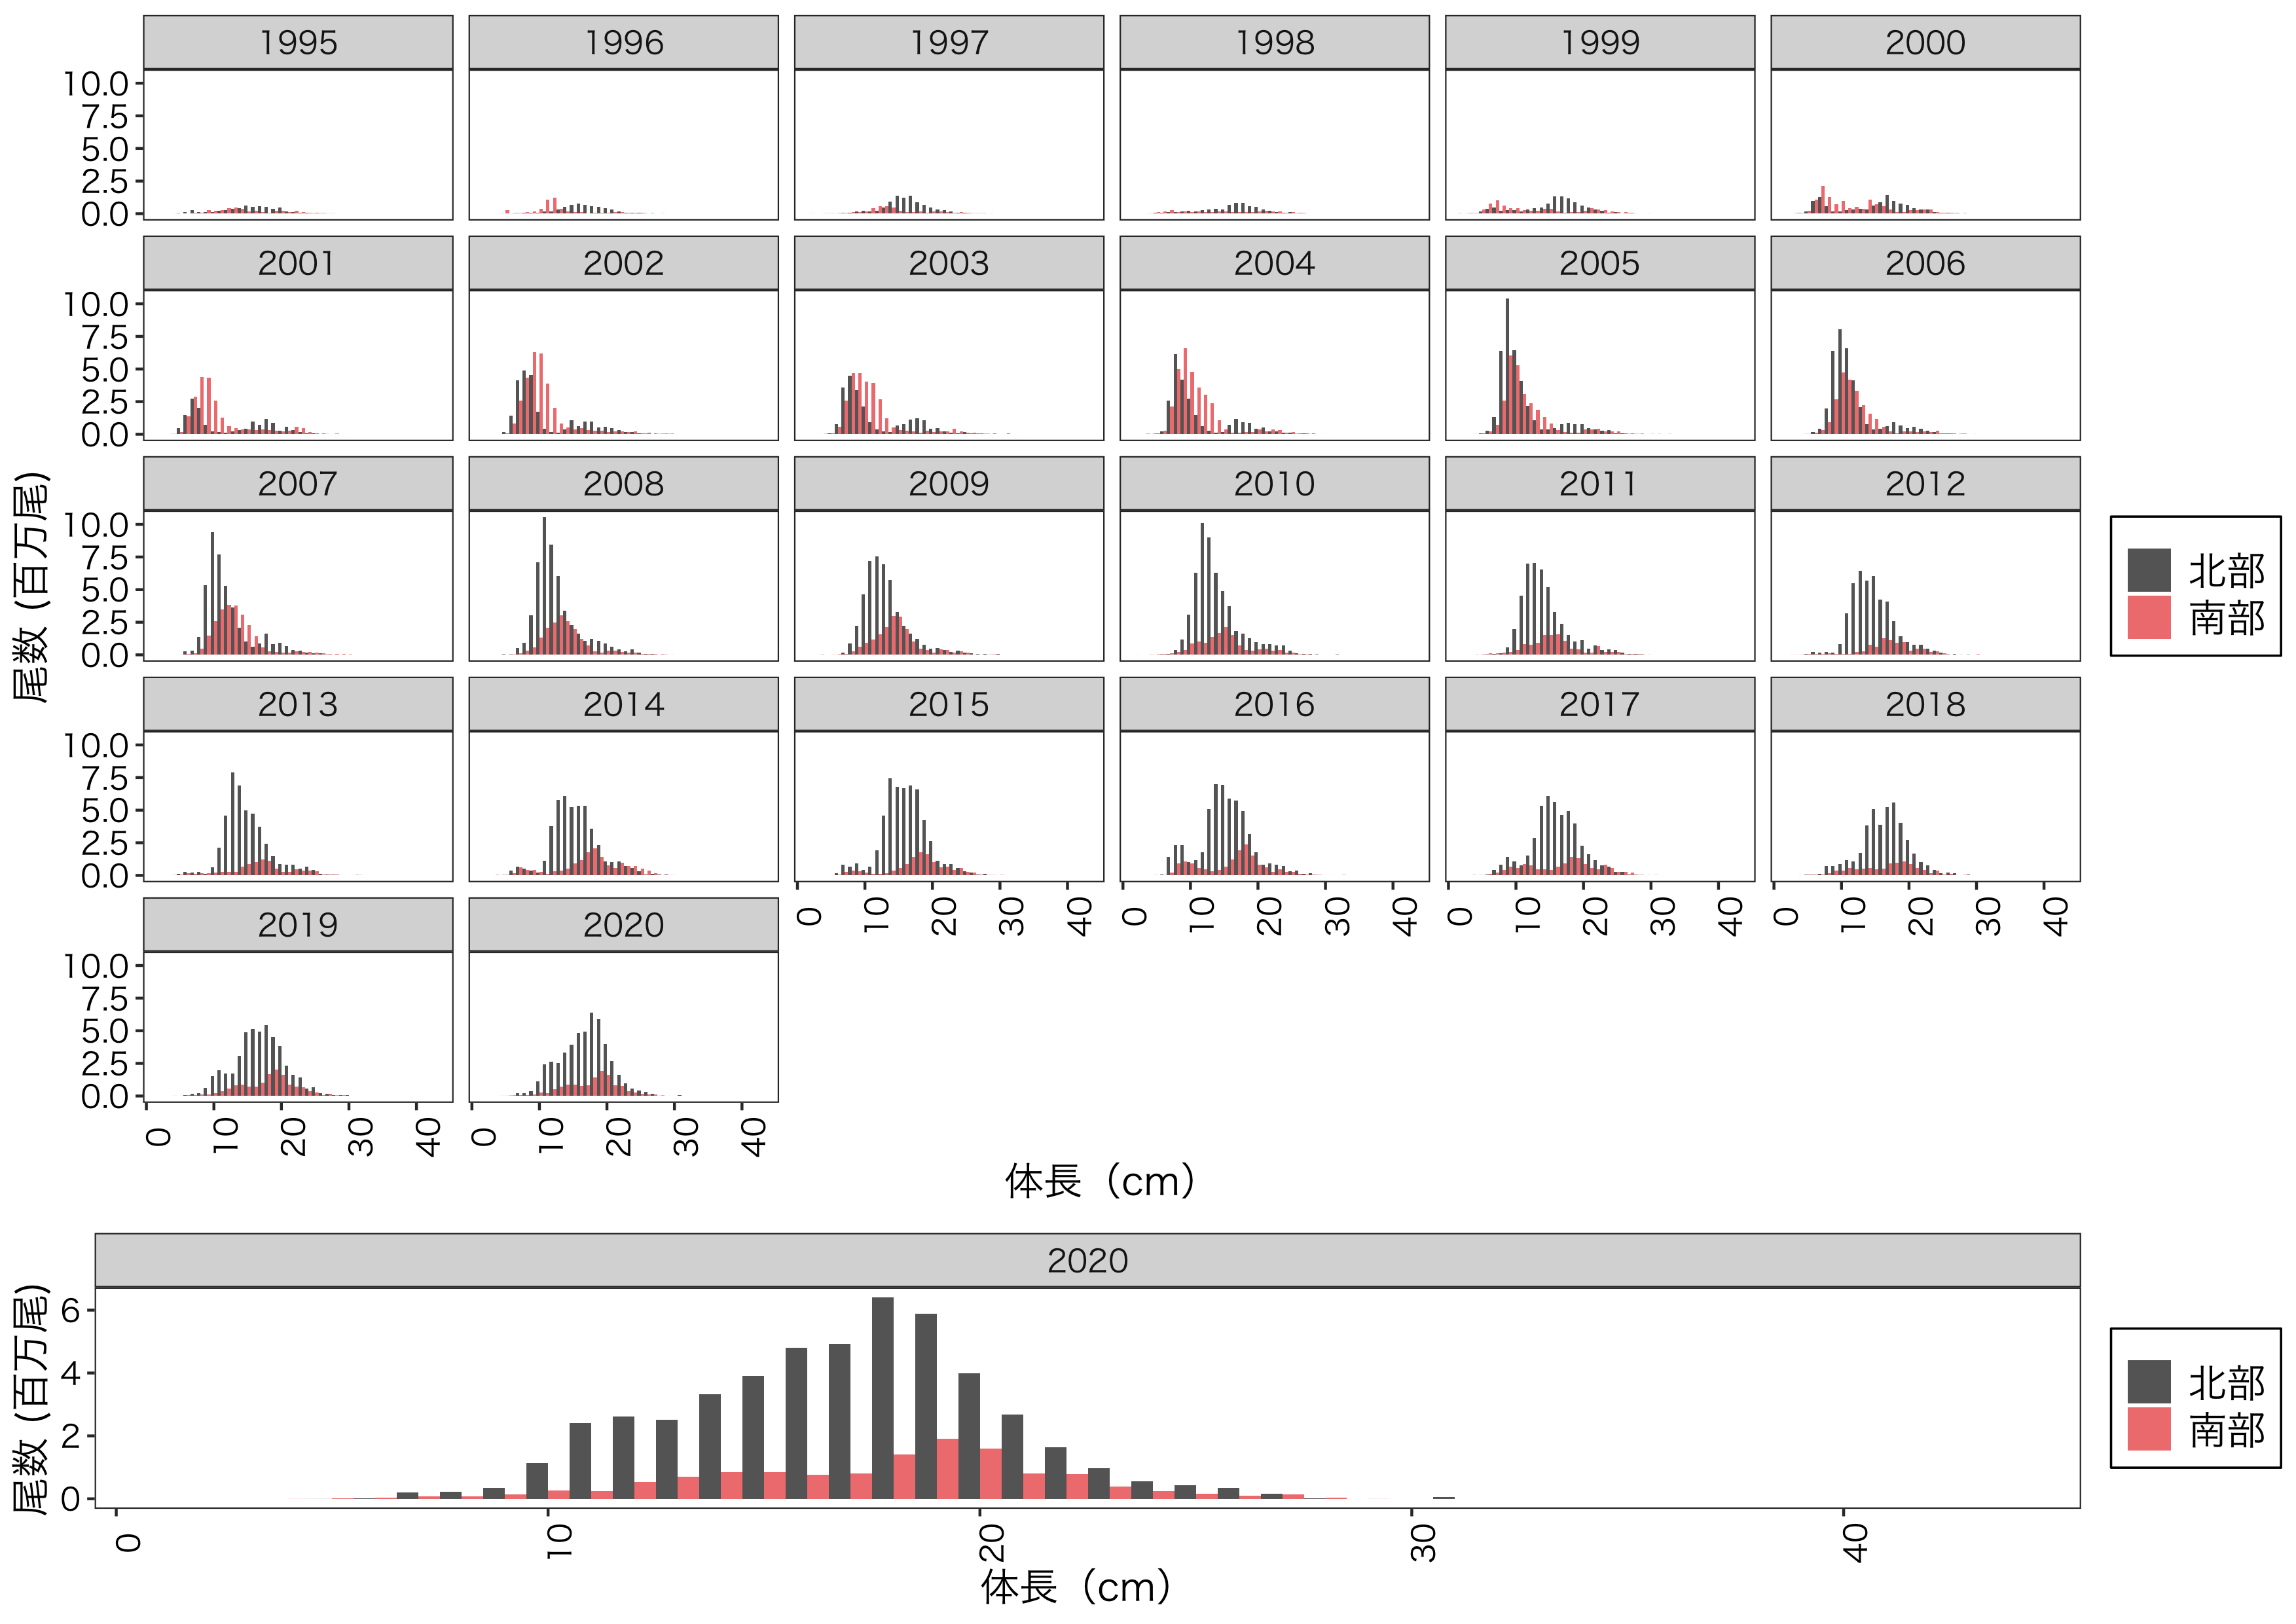
\includegraphics[width = 14cm]{キチジlength.png}
  \caption{キチジの体長組成の経年変化}
\end{figure}

\begin{figure}[h]
  \centering
  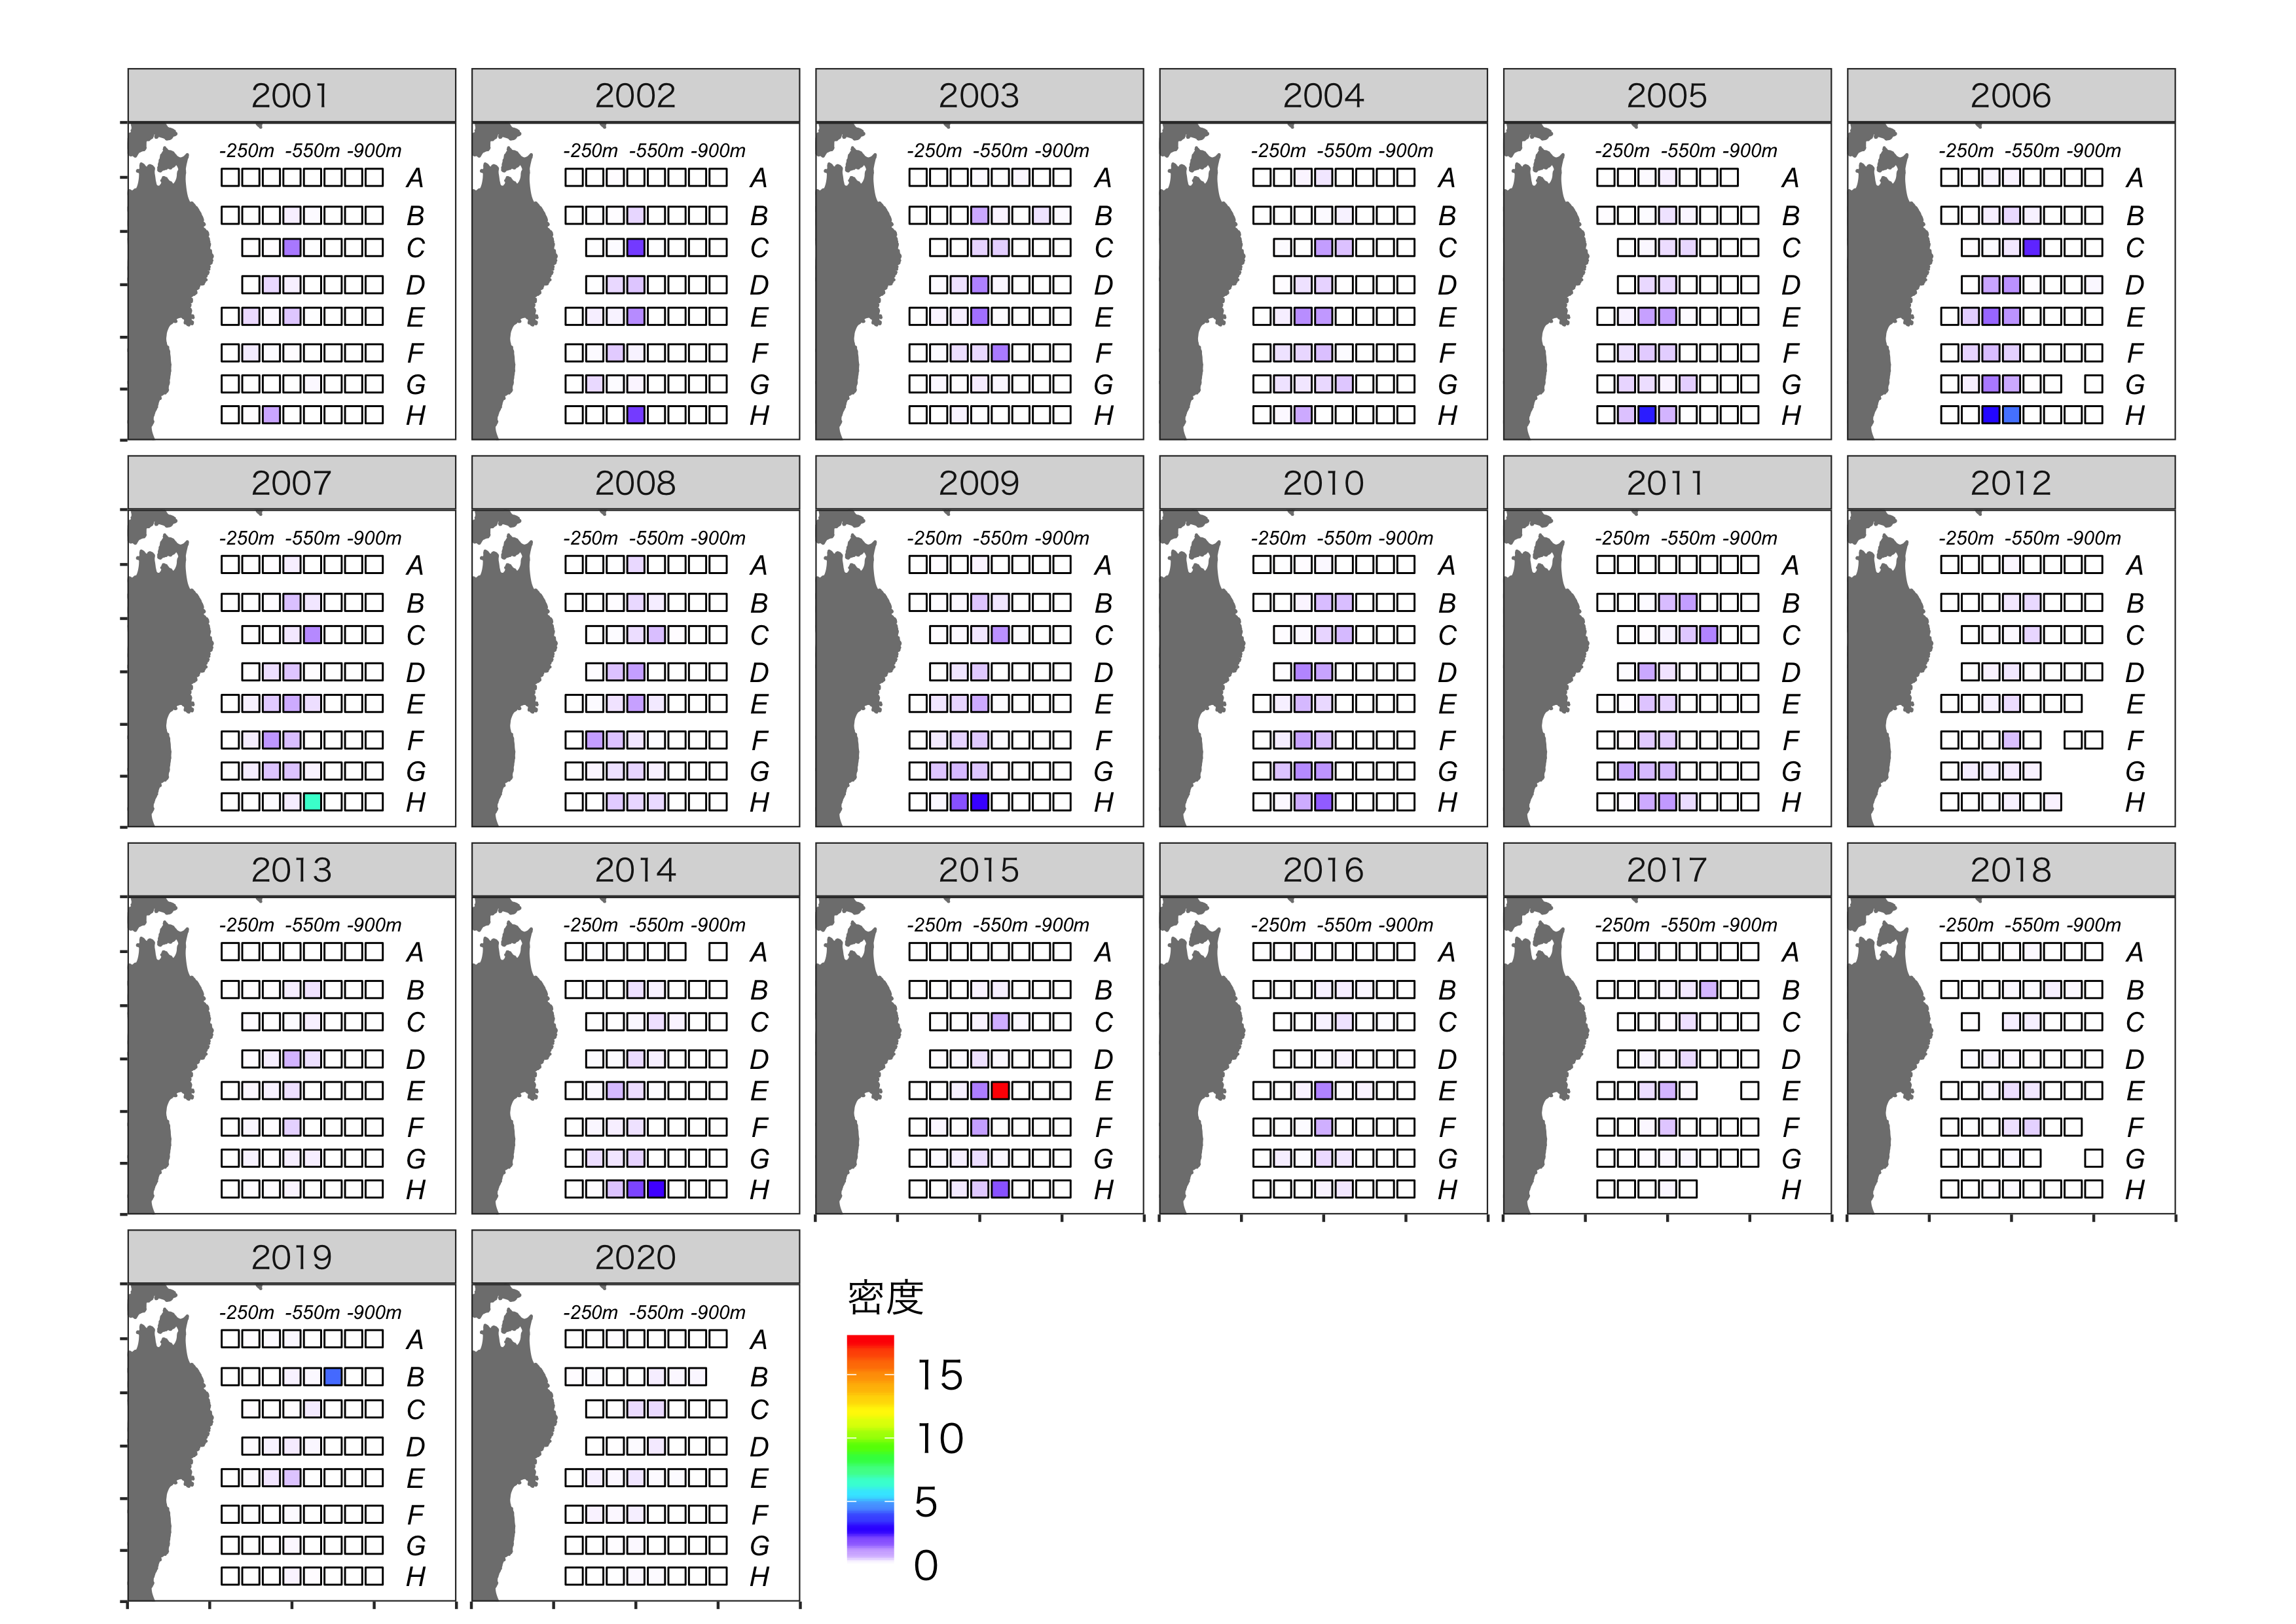
\includegraphics[width = 14cm]{ズワイガニ雌dens.png}
  \caption{ズワイガニ雌の分布密度(千尾/km2)の経年変化}
\end{figure}

\begin{figure}[h]
  \centering
  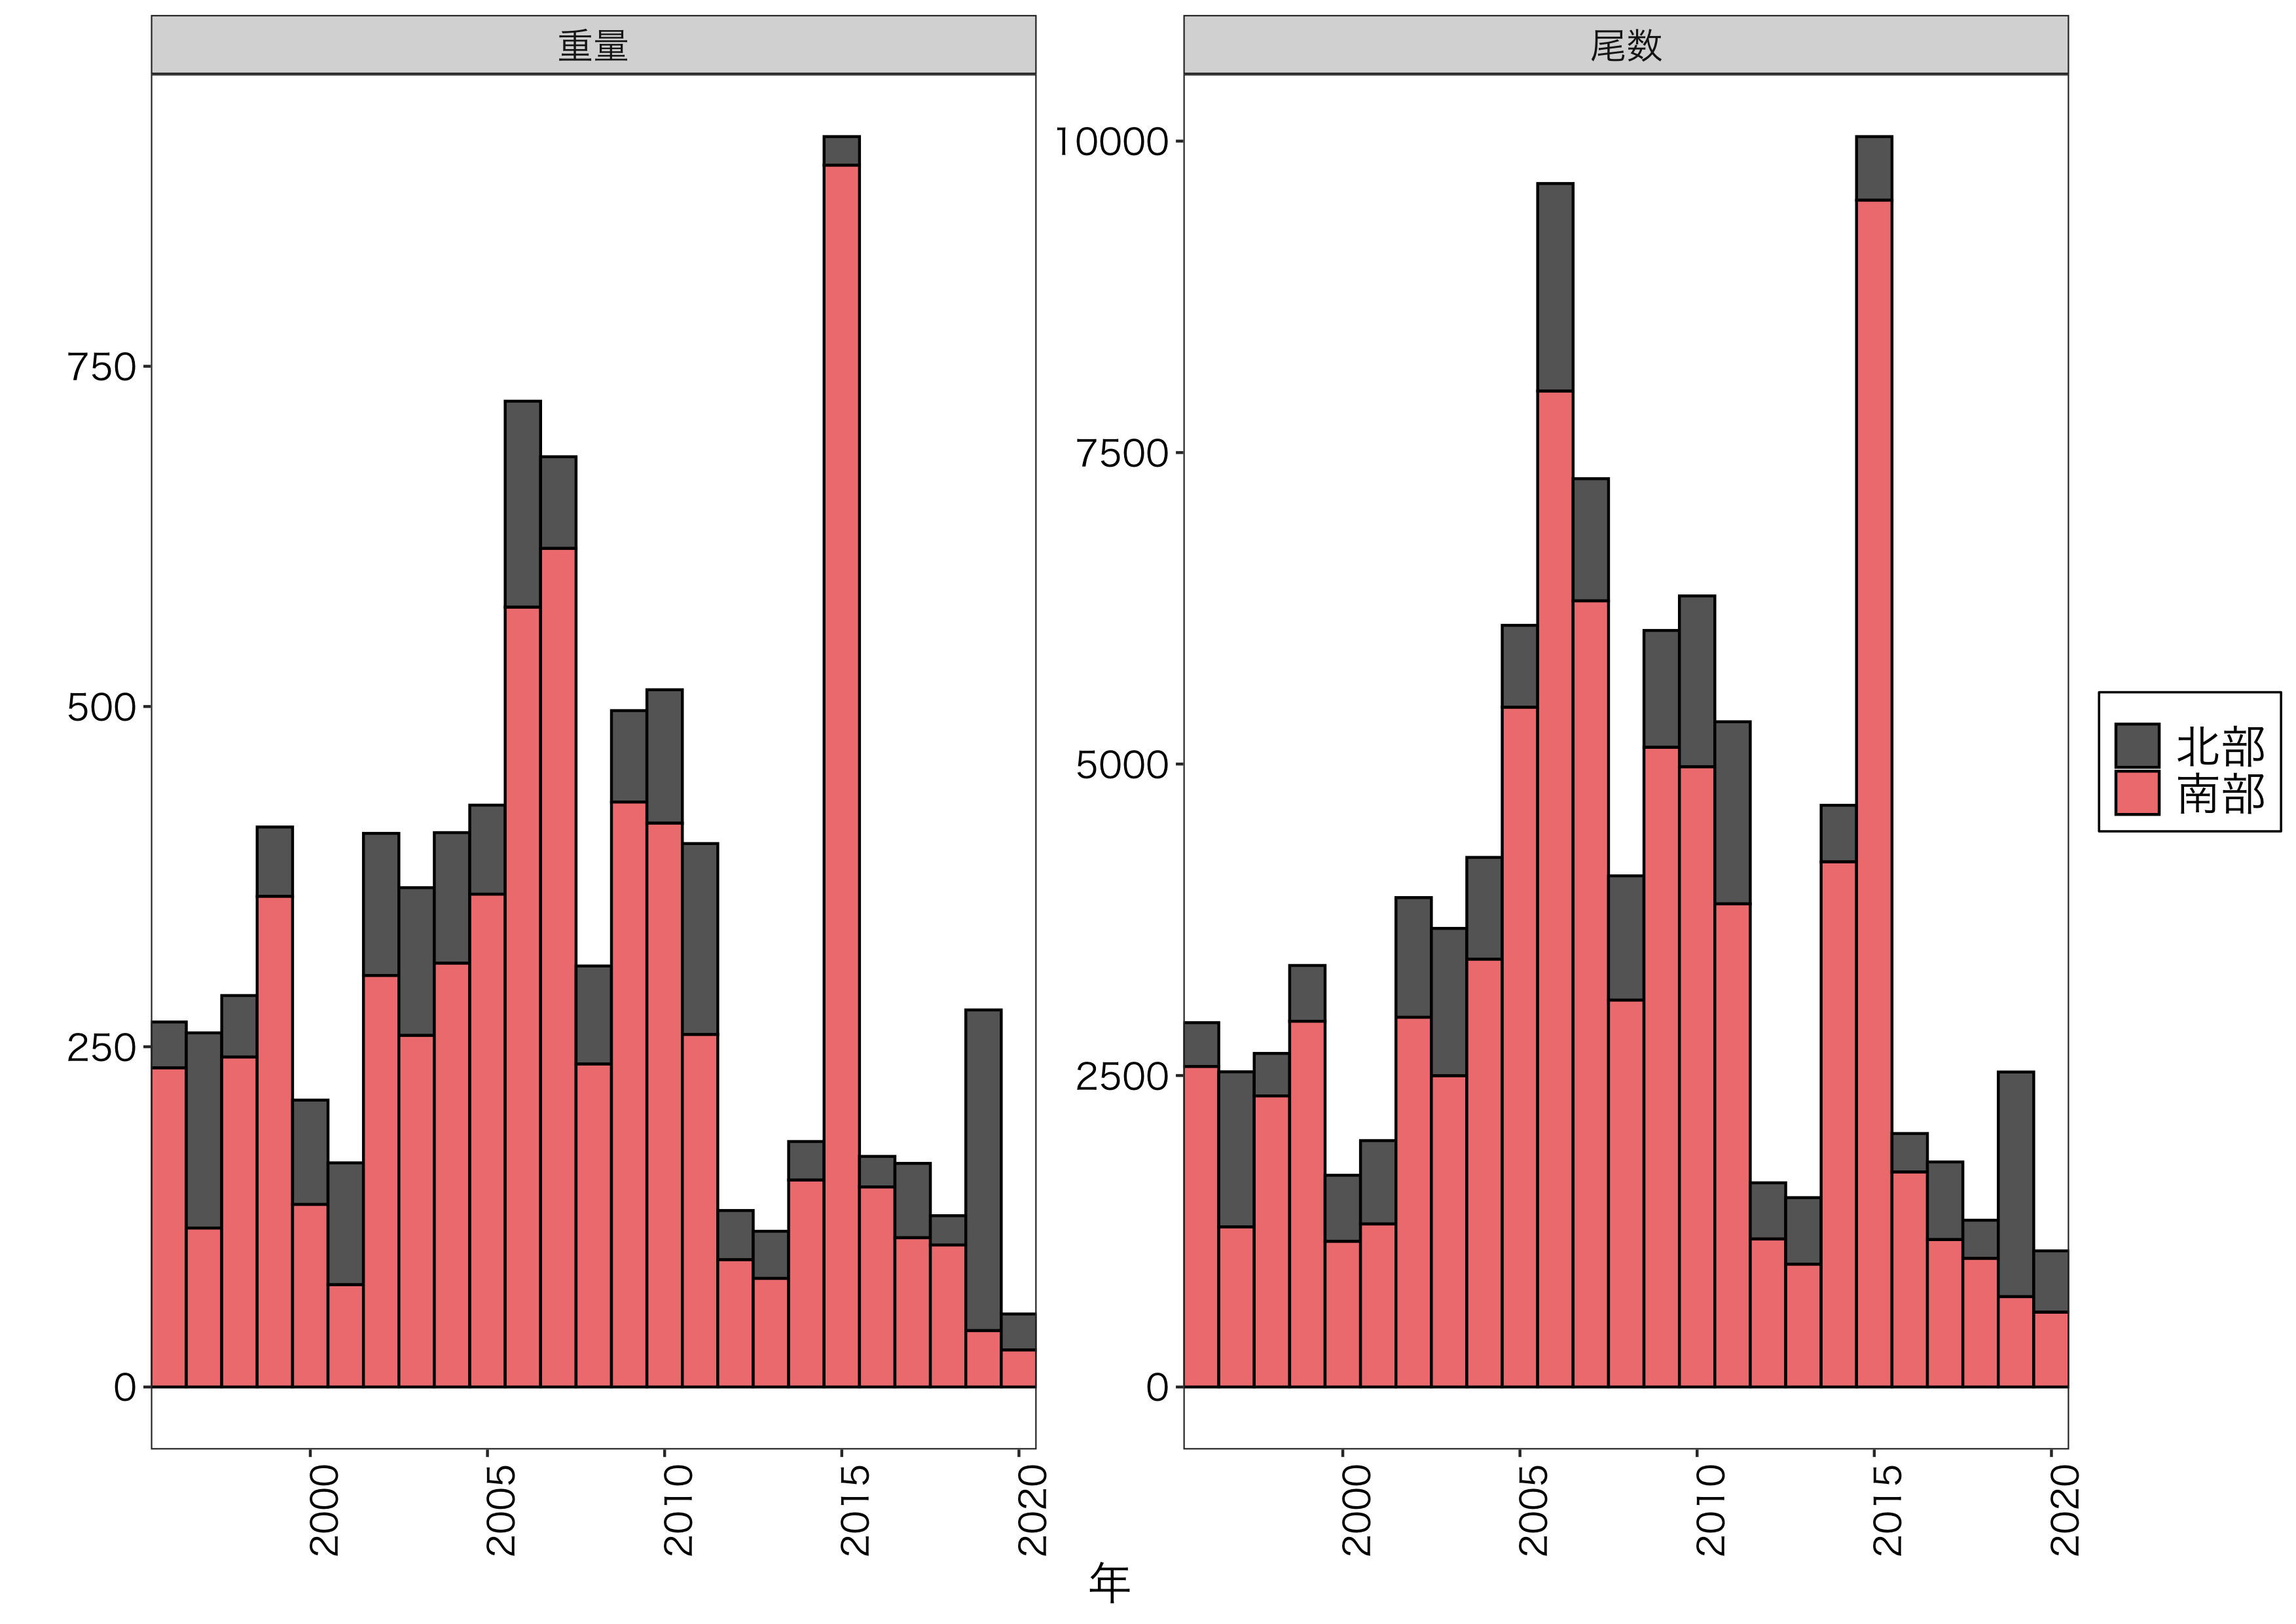
\includegraphics[width = 14cm]{ズワイガニ雌trend.png}
  \caption{ズワイガニ雌の現存量(右; 単位は千トン)と現存尾数(左; 単位は百万尾)の経年変化}
\end{figure}

\begin{figure}[h]
  \centering
  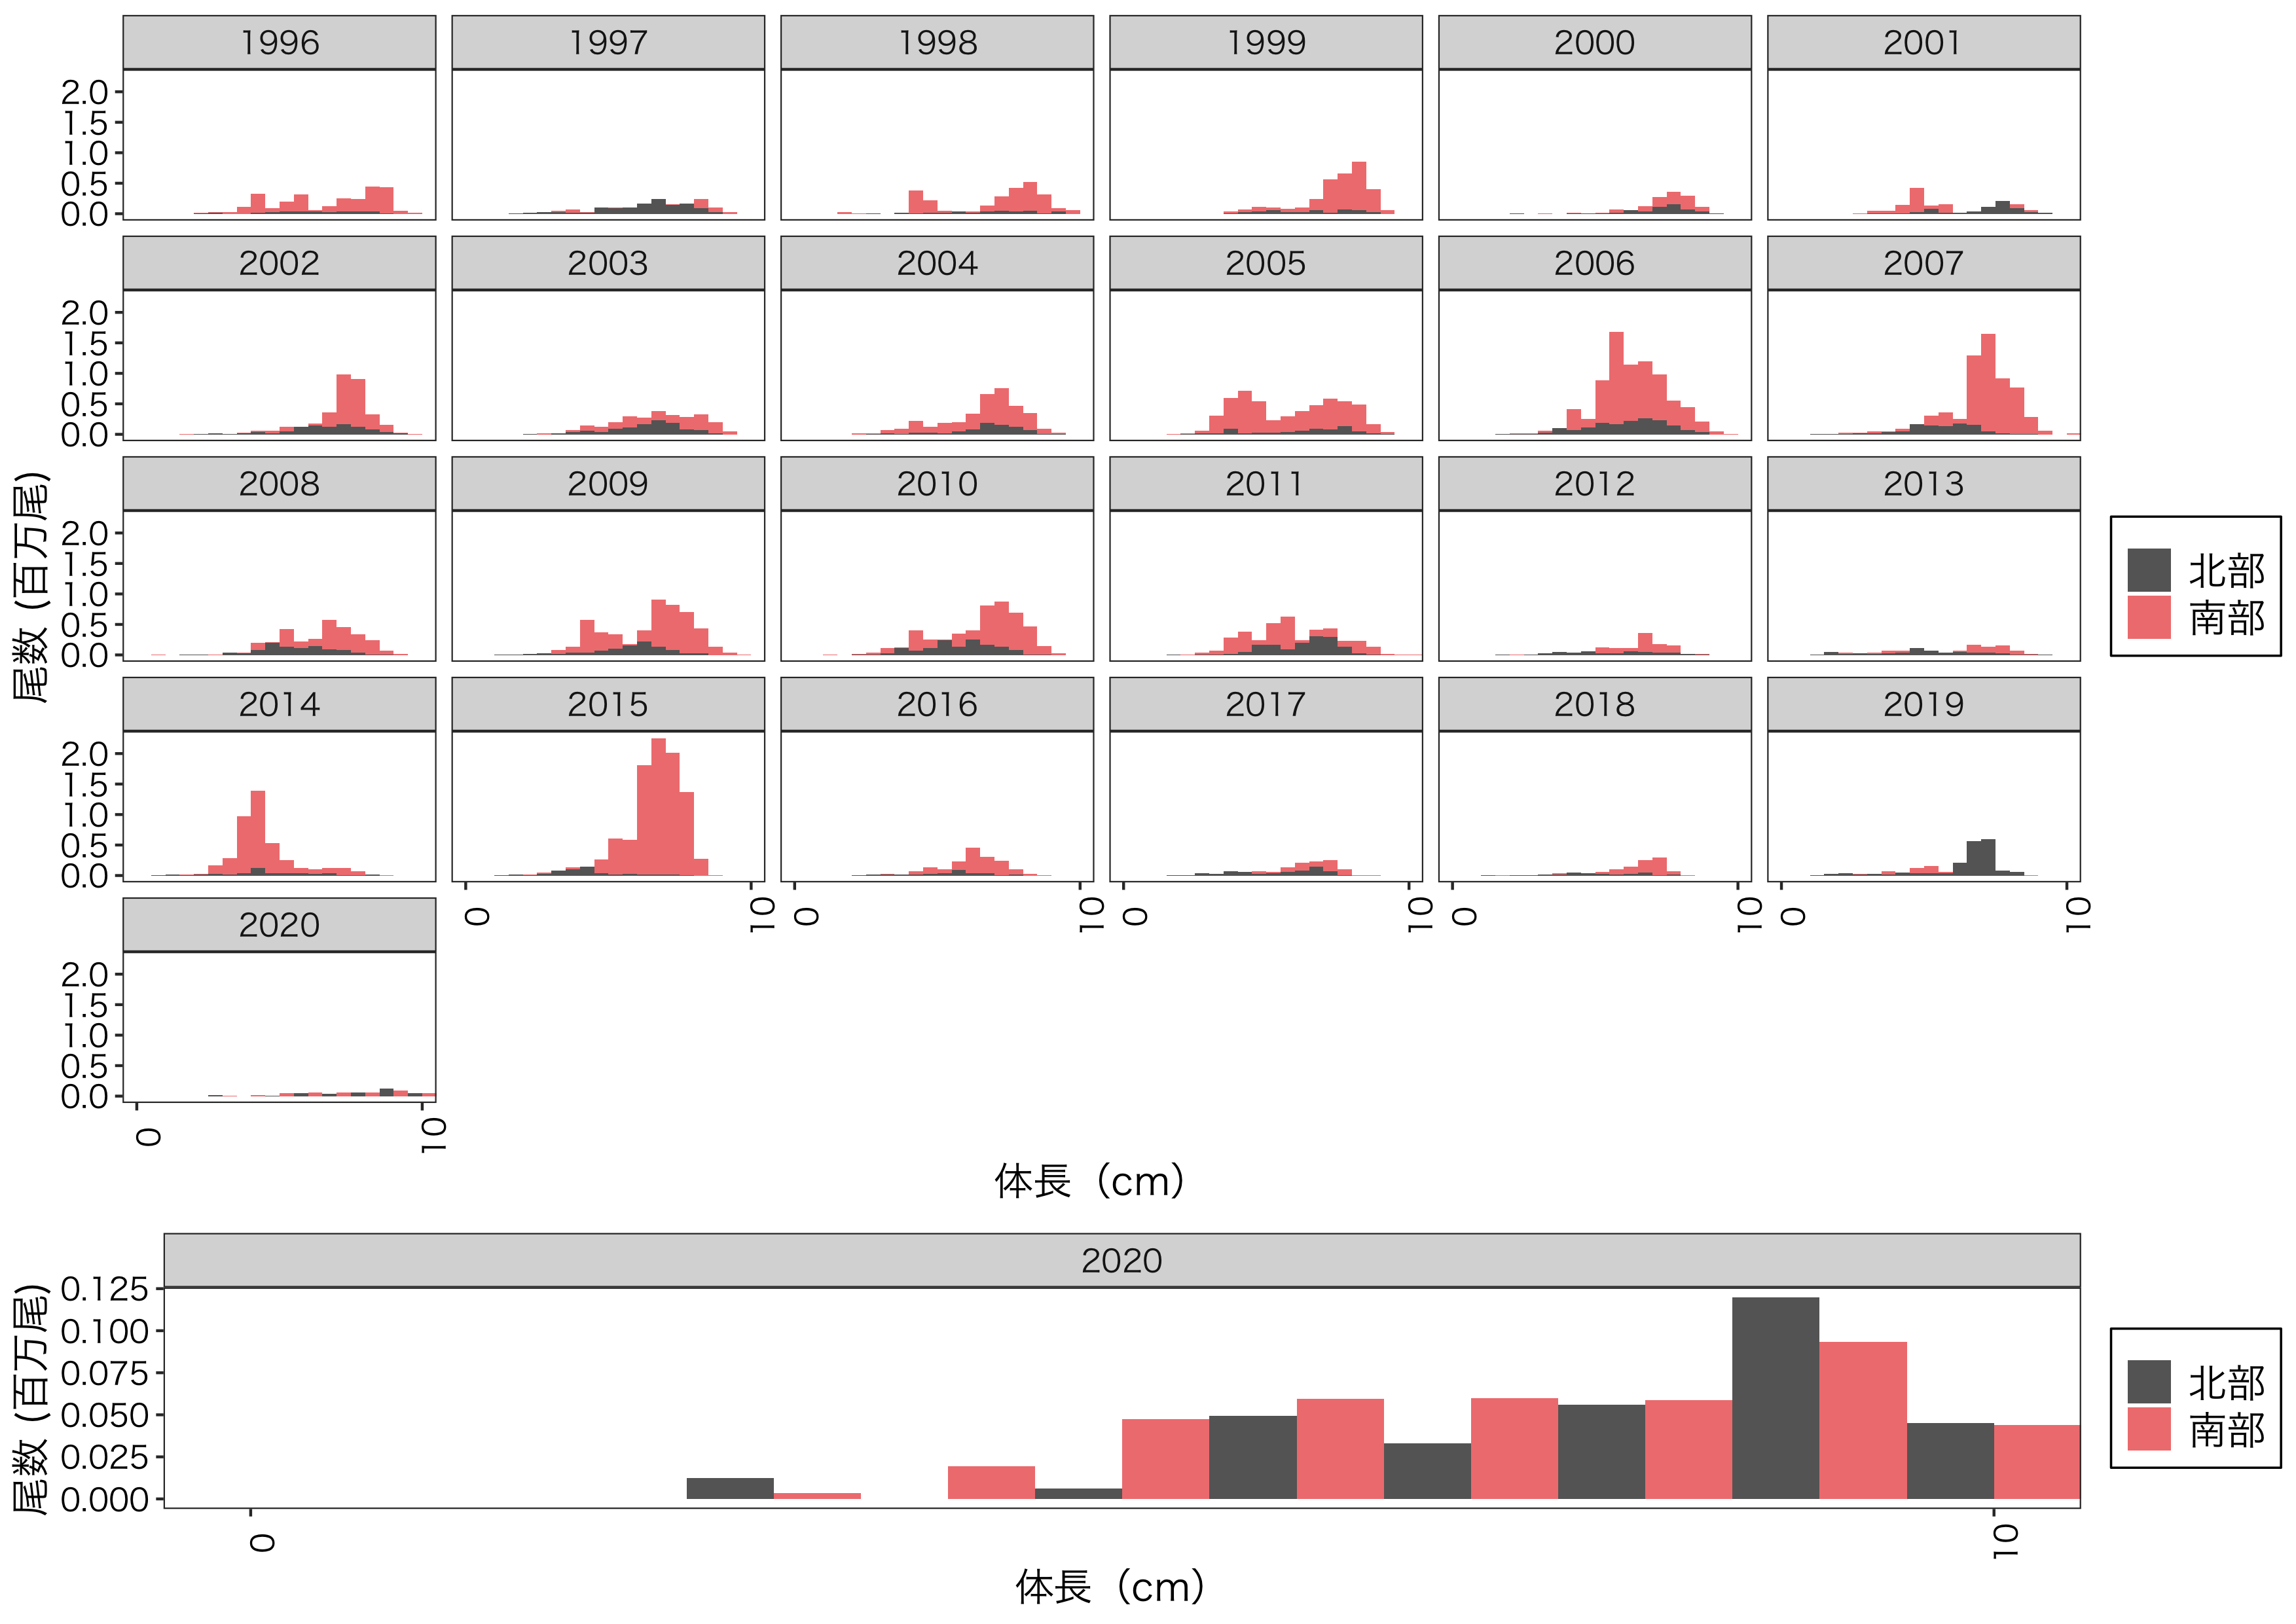
\includegraphics[width = 14cm]{ズワイガニ雌length.png}
  \caption{ズワイガニ雌の体長組成の経年変化}
\end{figure}

\begin{figure}[h]
  \centering
  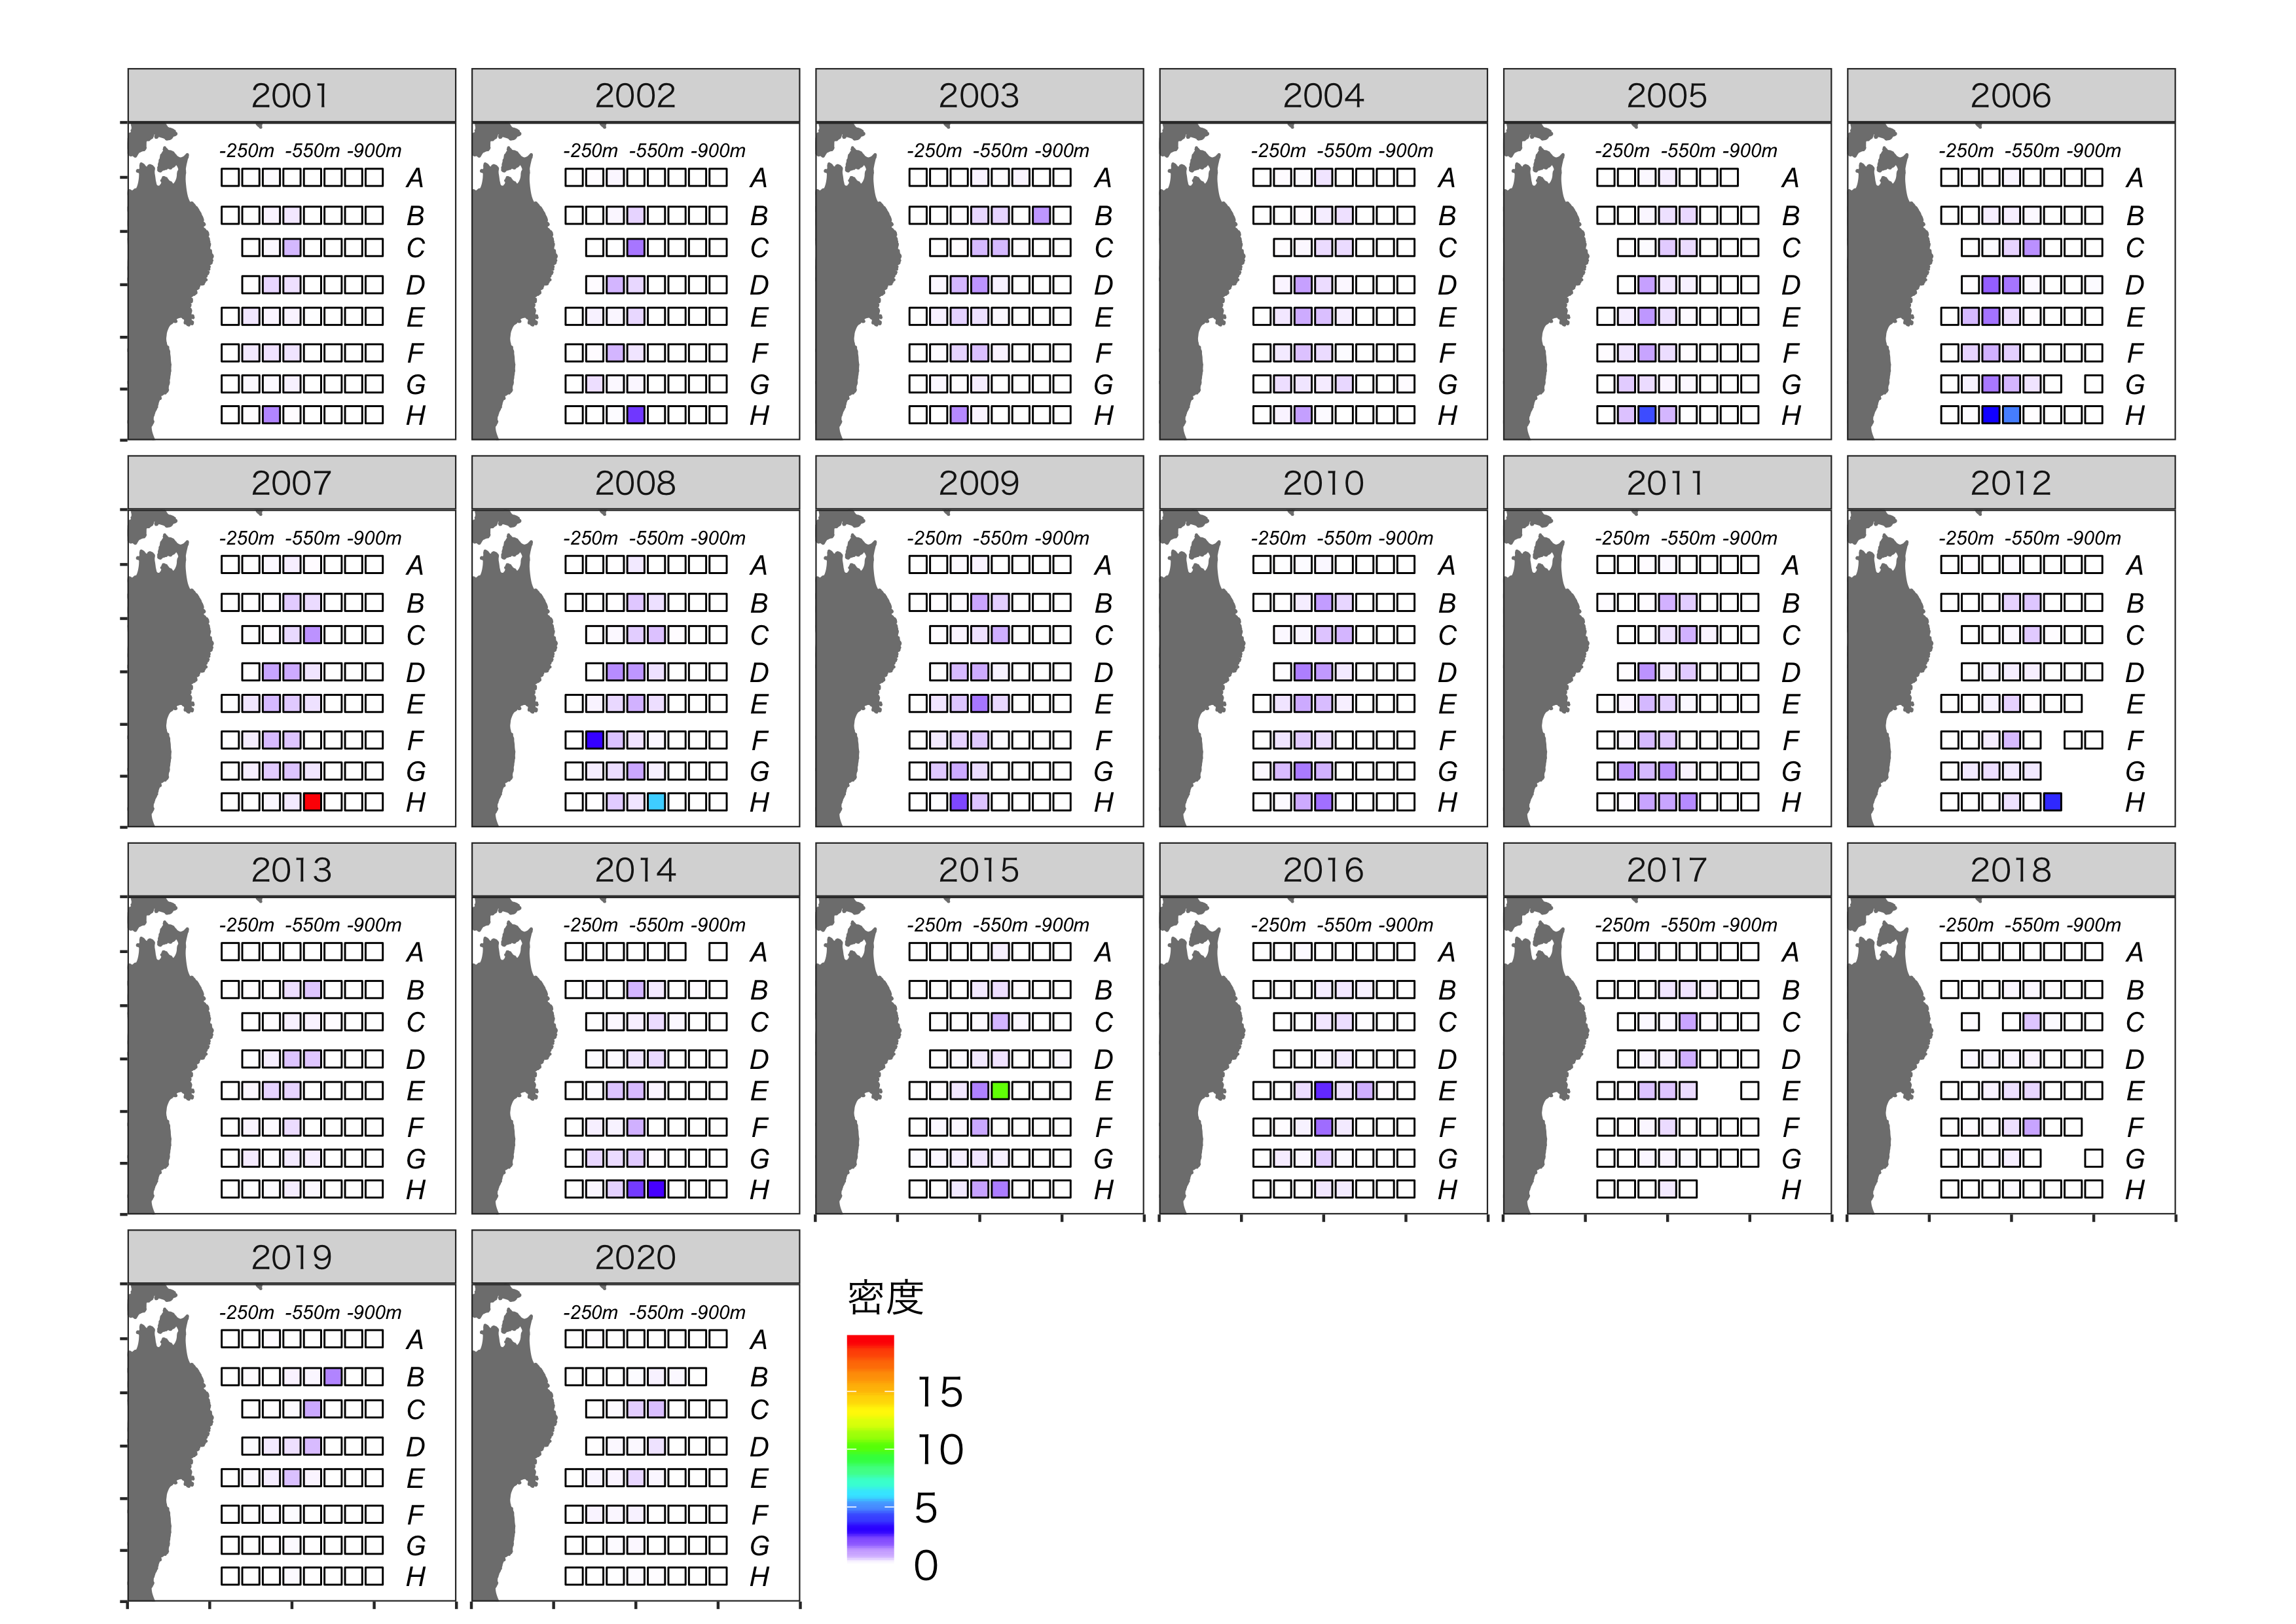
\includegraphics[width = 14cm]{ズワイガニ雄dens.png}
  \caption{ズワイガニ雄の分布密度(千尾/km2)の経年変化}
\end{figure}

\begin{figure}[h]
  \centering
  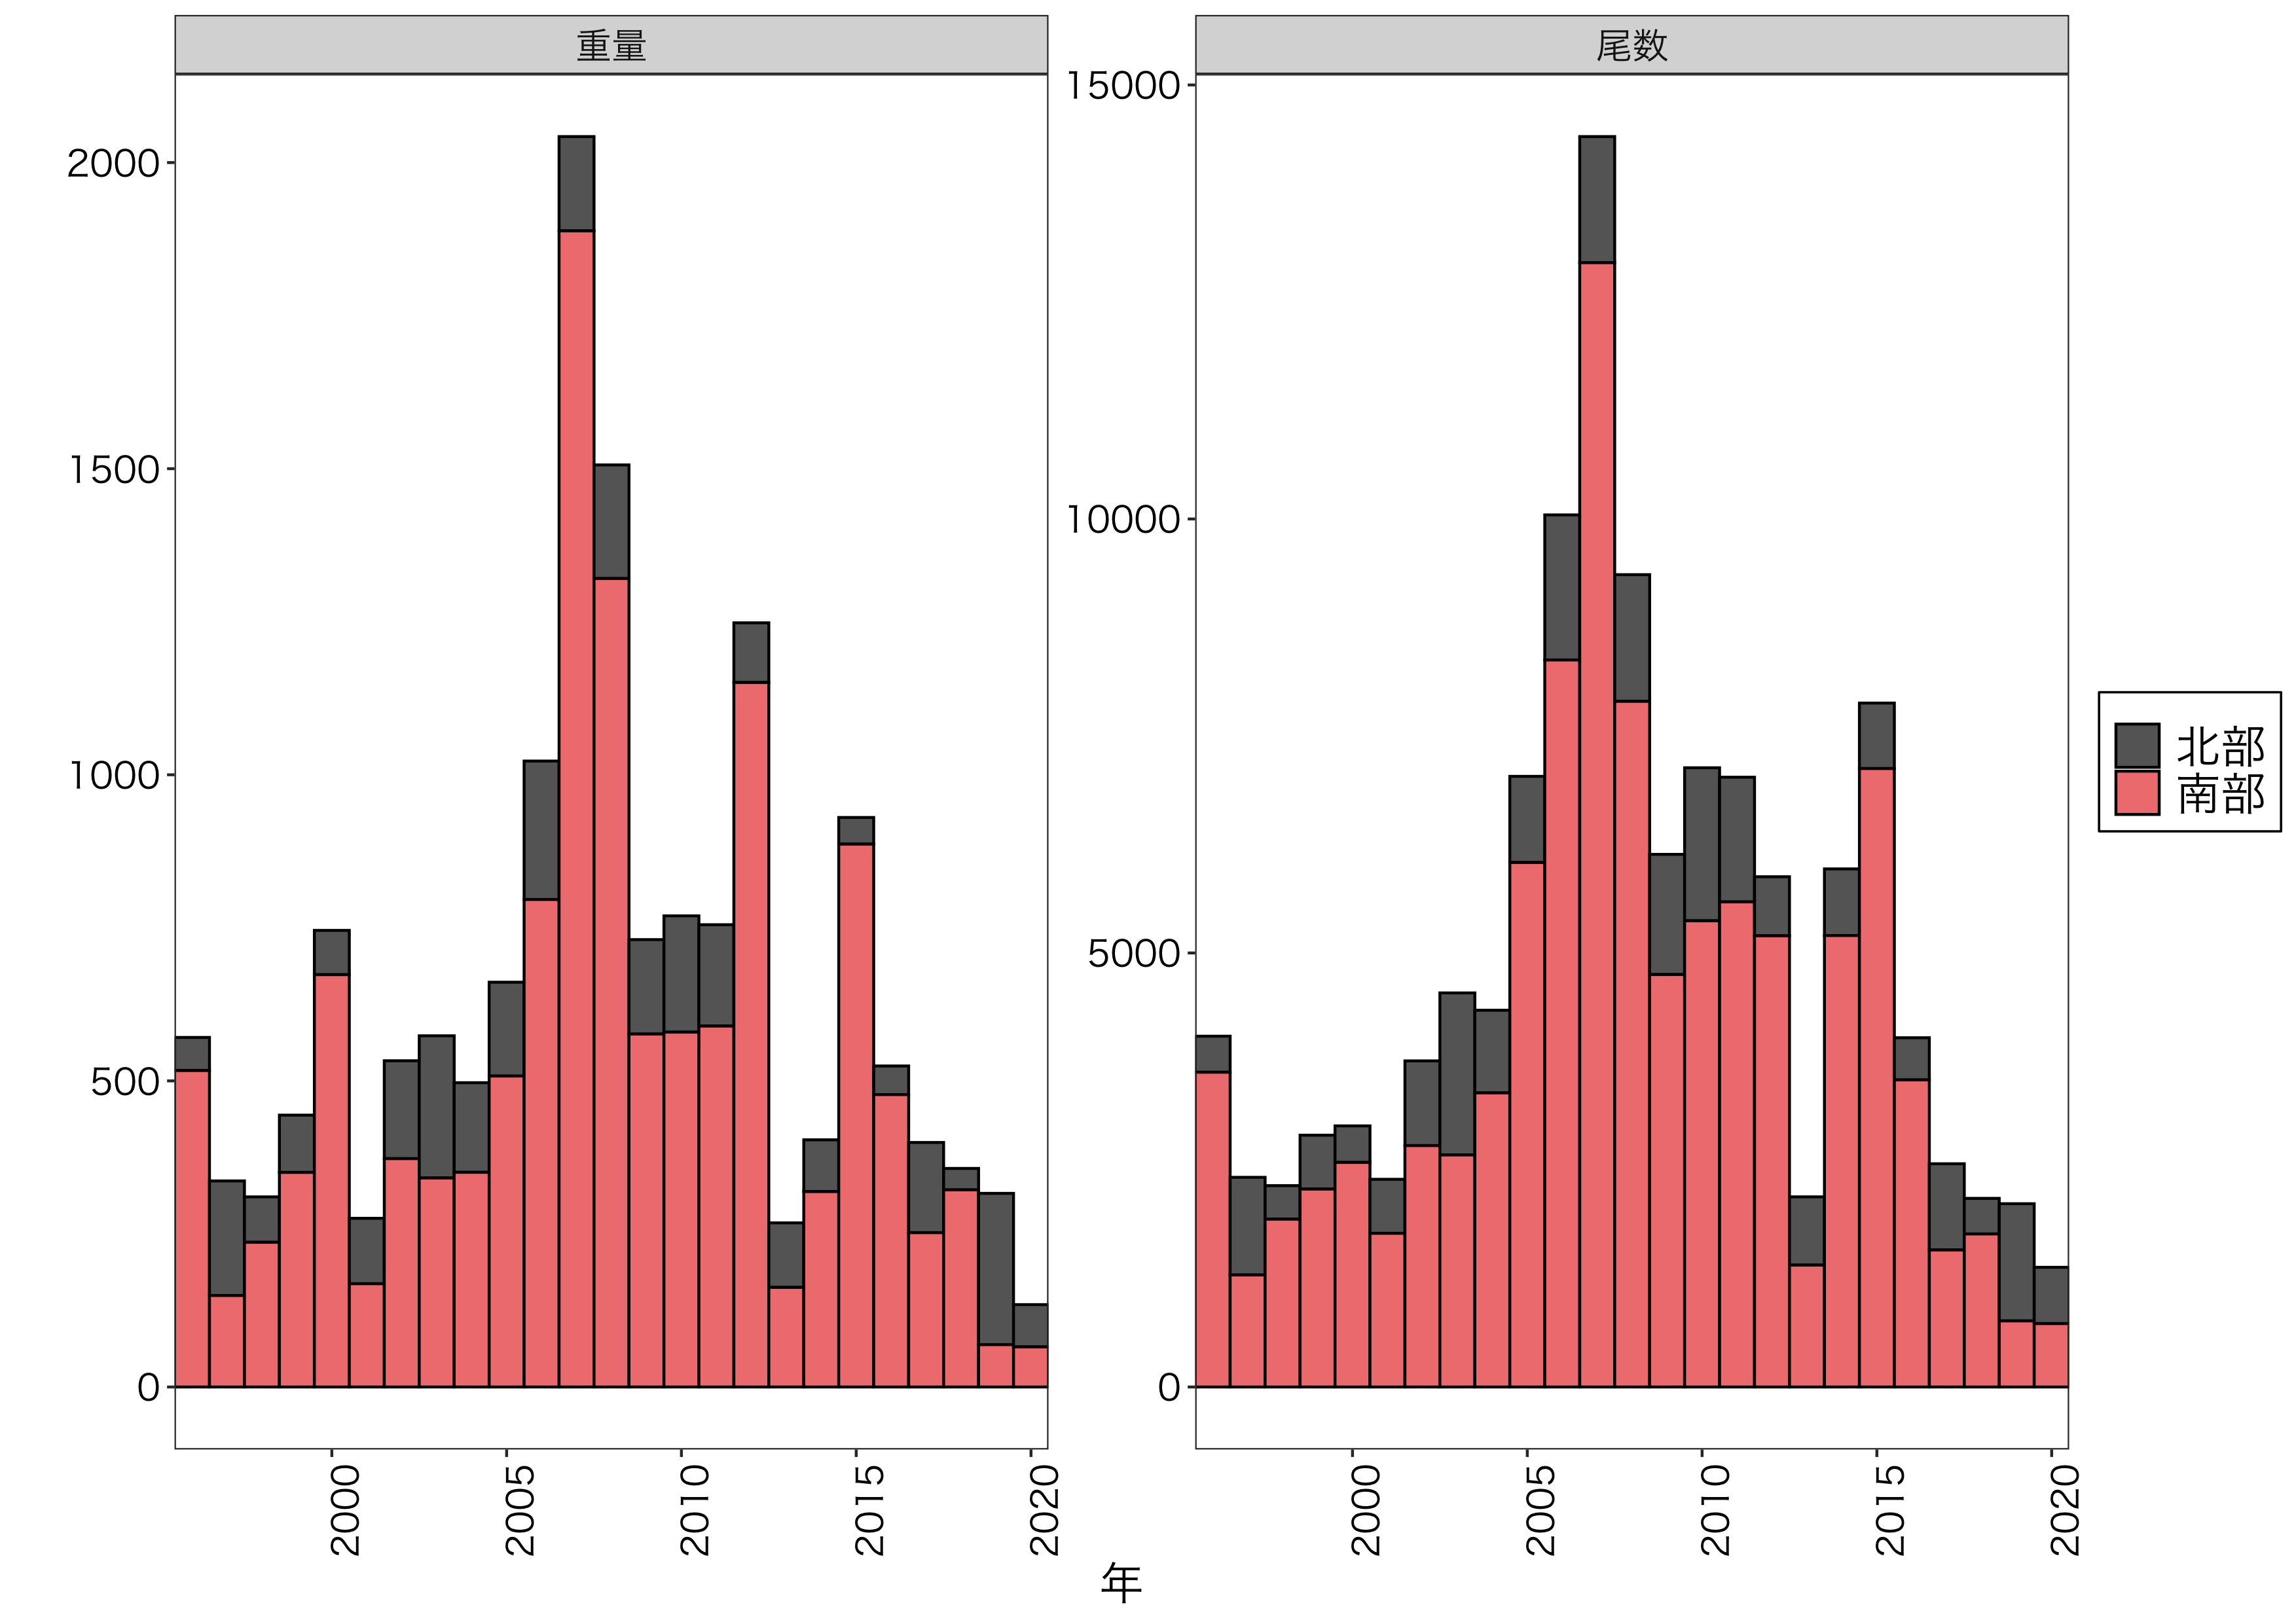
\includegraphics[width = 14cm]{ズワイガニ雄trend.png}
  \caption{ズワイガニ雄の現存量(右; 単位は千トン)と現存尾数(左; 単位は百万尾)の経年変化}
\end{figure}

\begin{figure}[h]
  \centering
  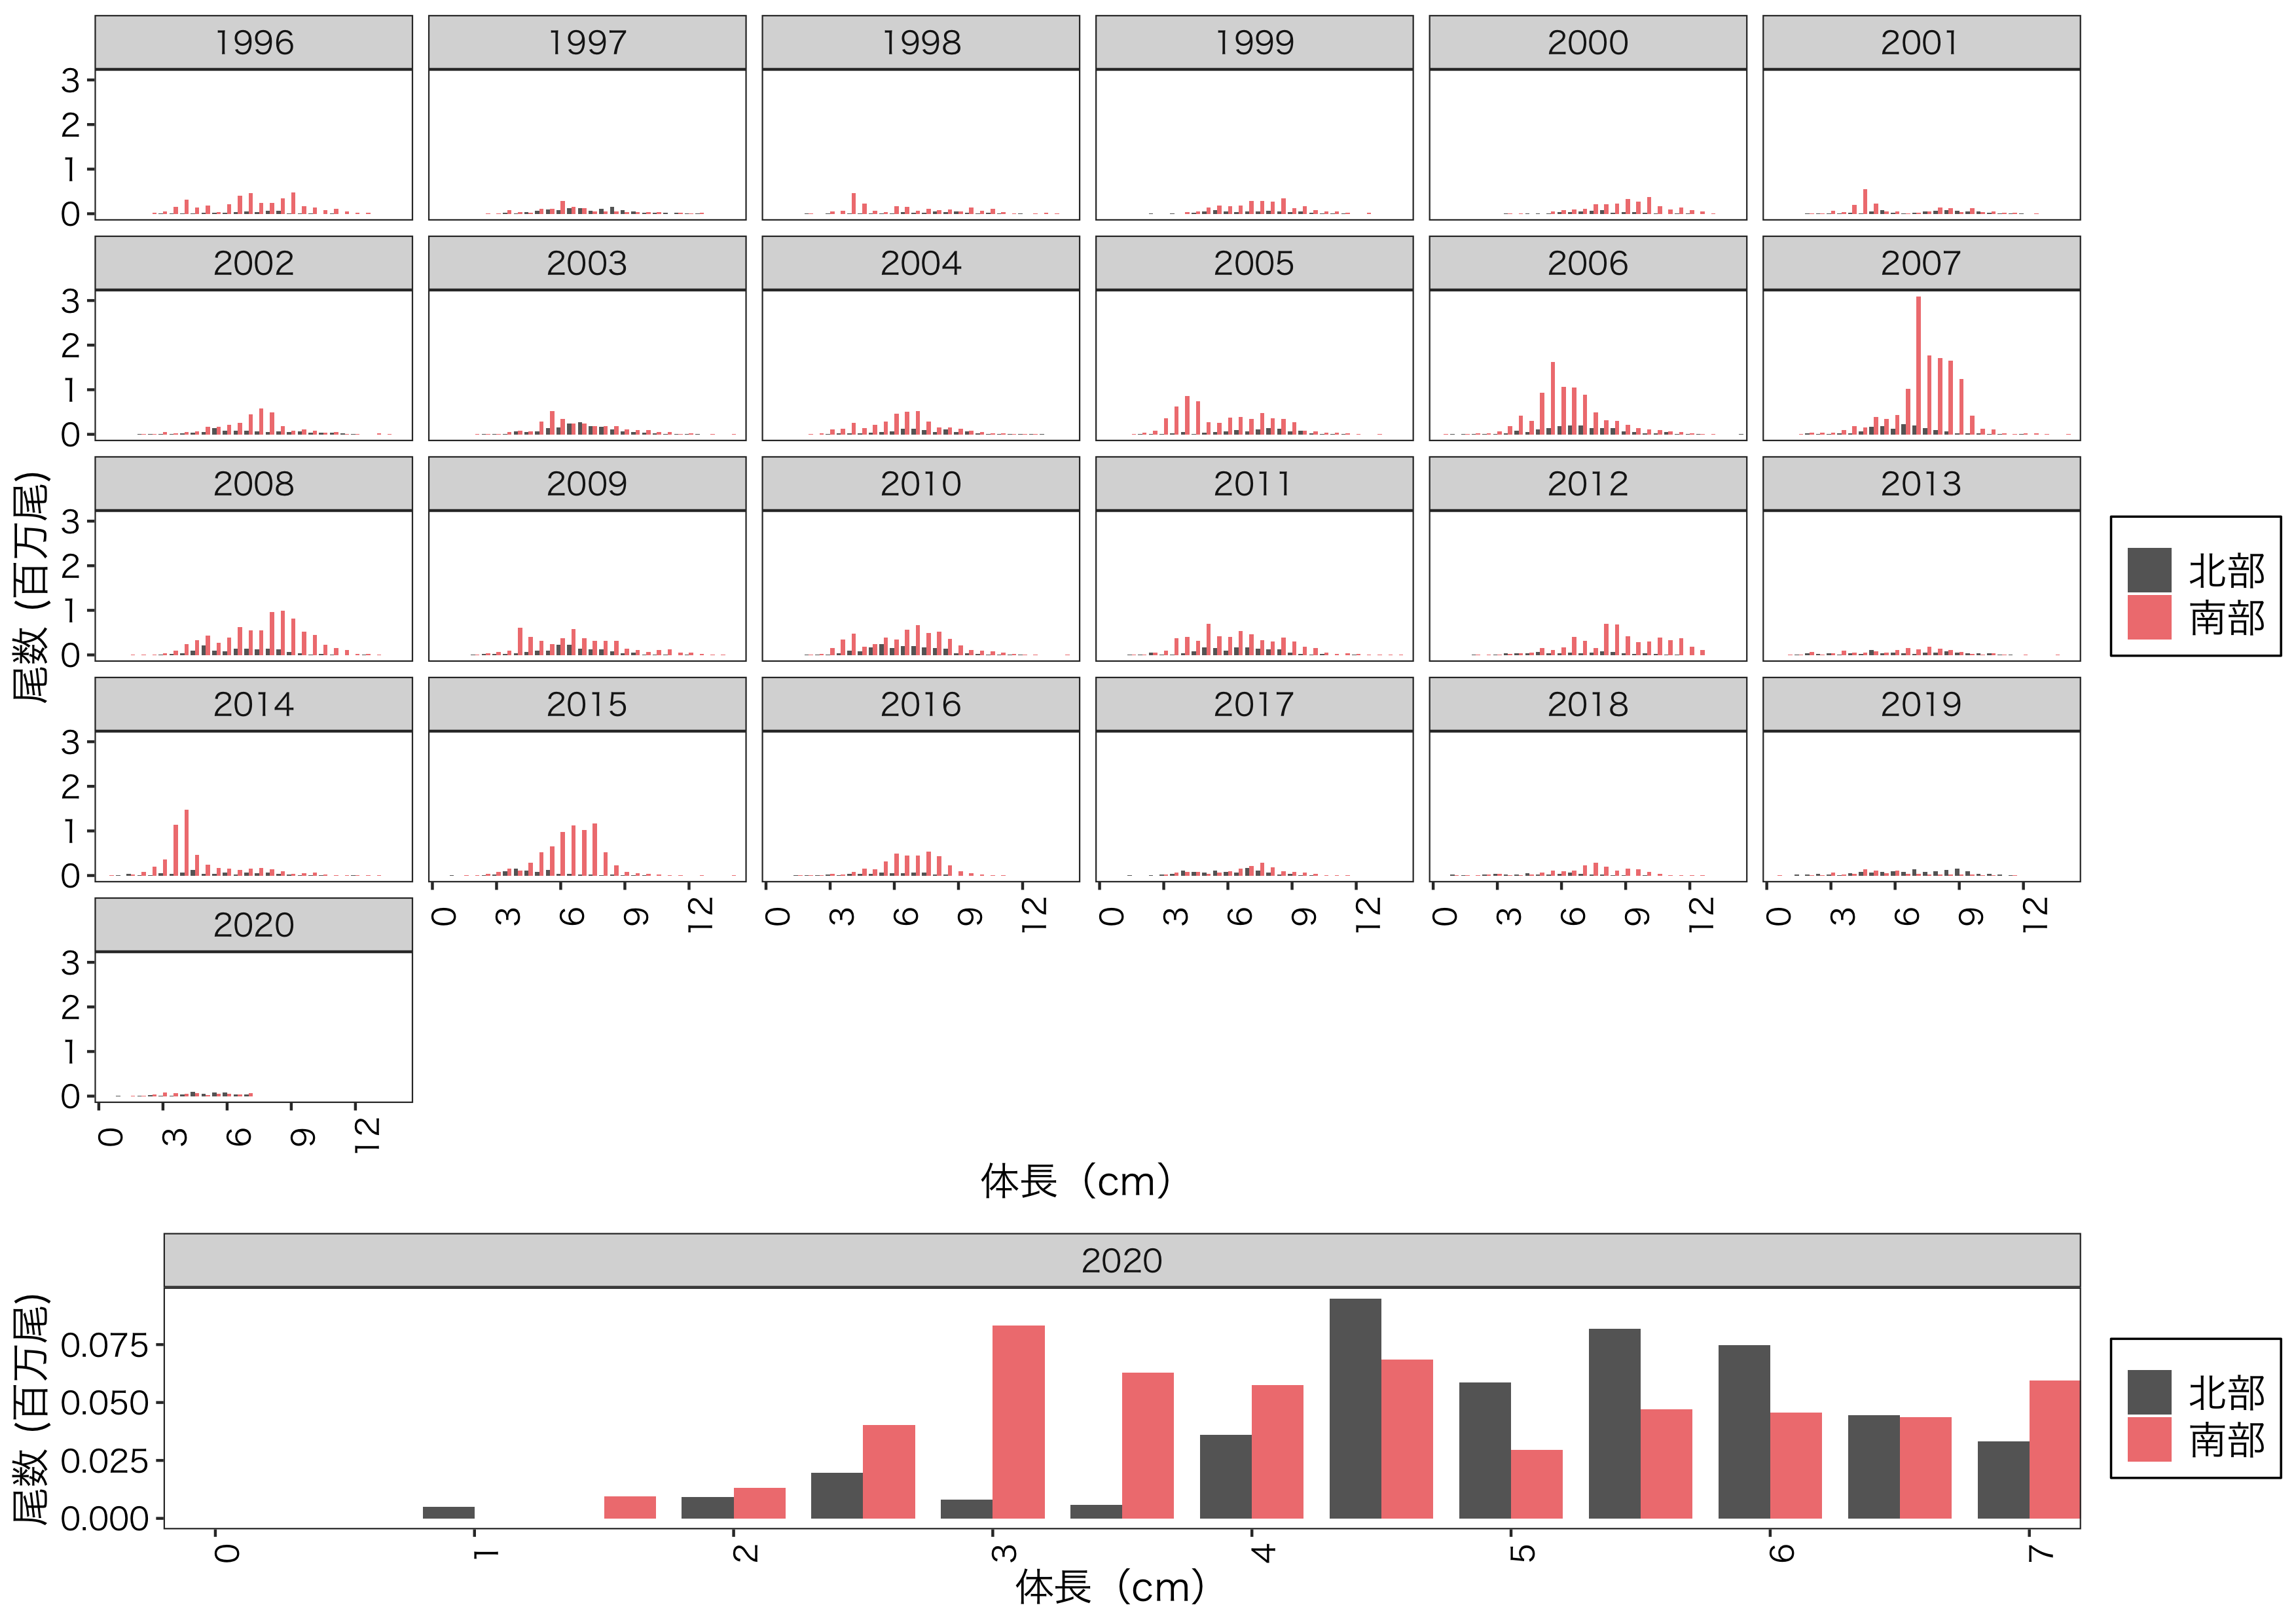
\includegraphics[width = 14cm]{ズワイガニ雄length.png}
  \caption{ズワイガニ雄の体長組成の経年変化}
\end{figure}

\begin{figure}[h]
  \centering
  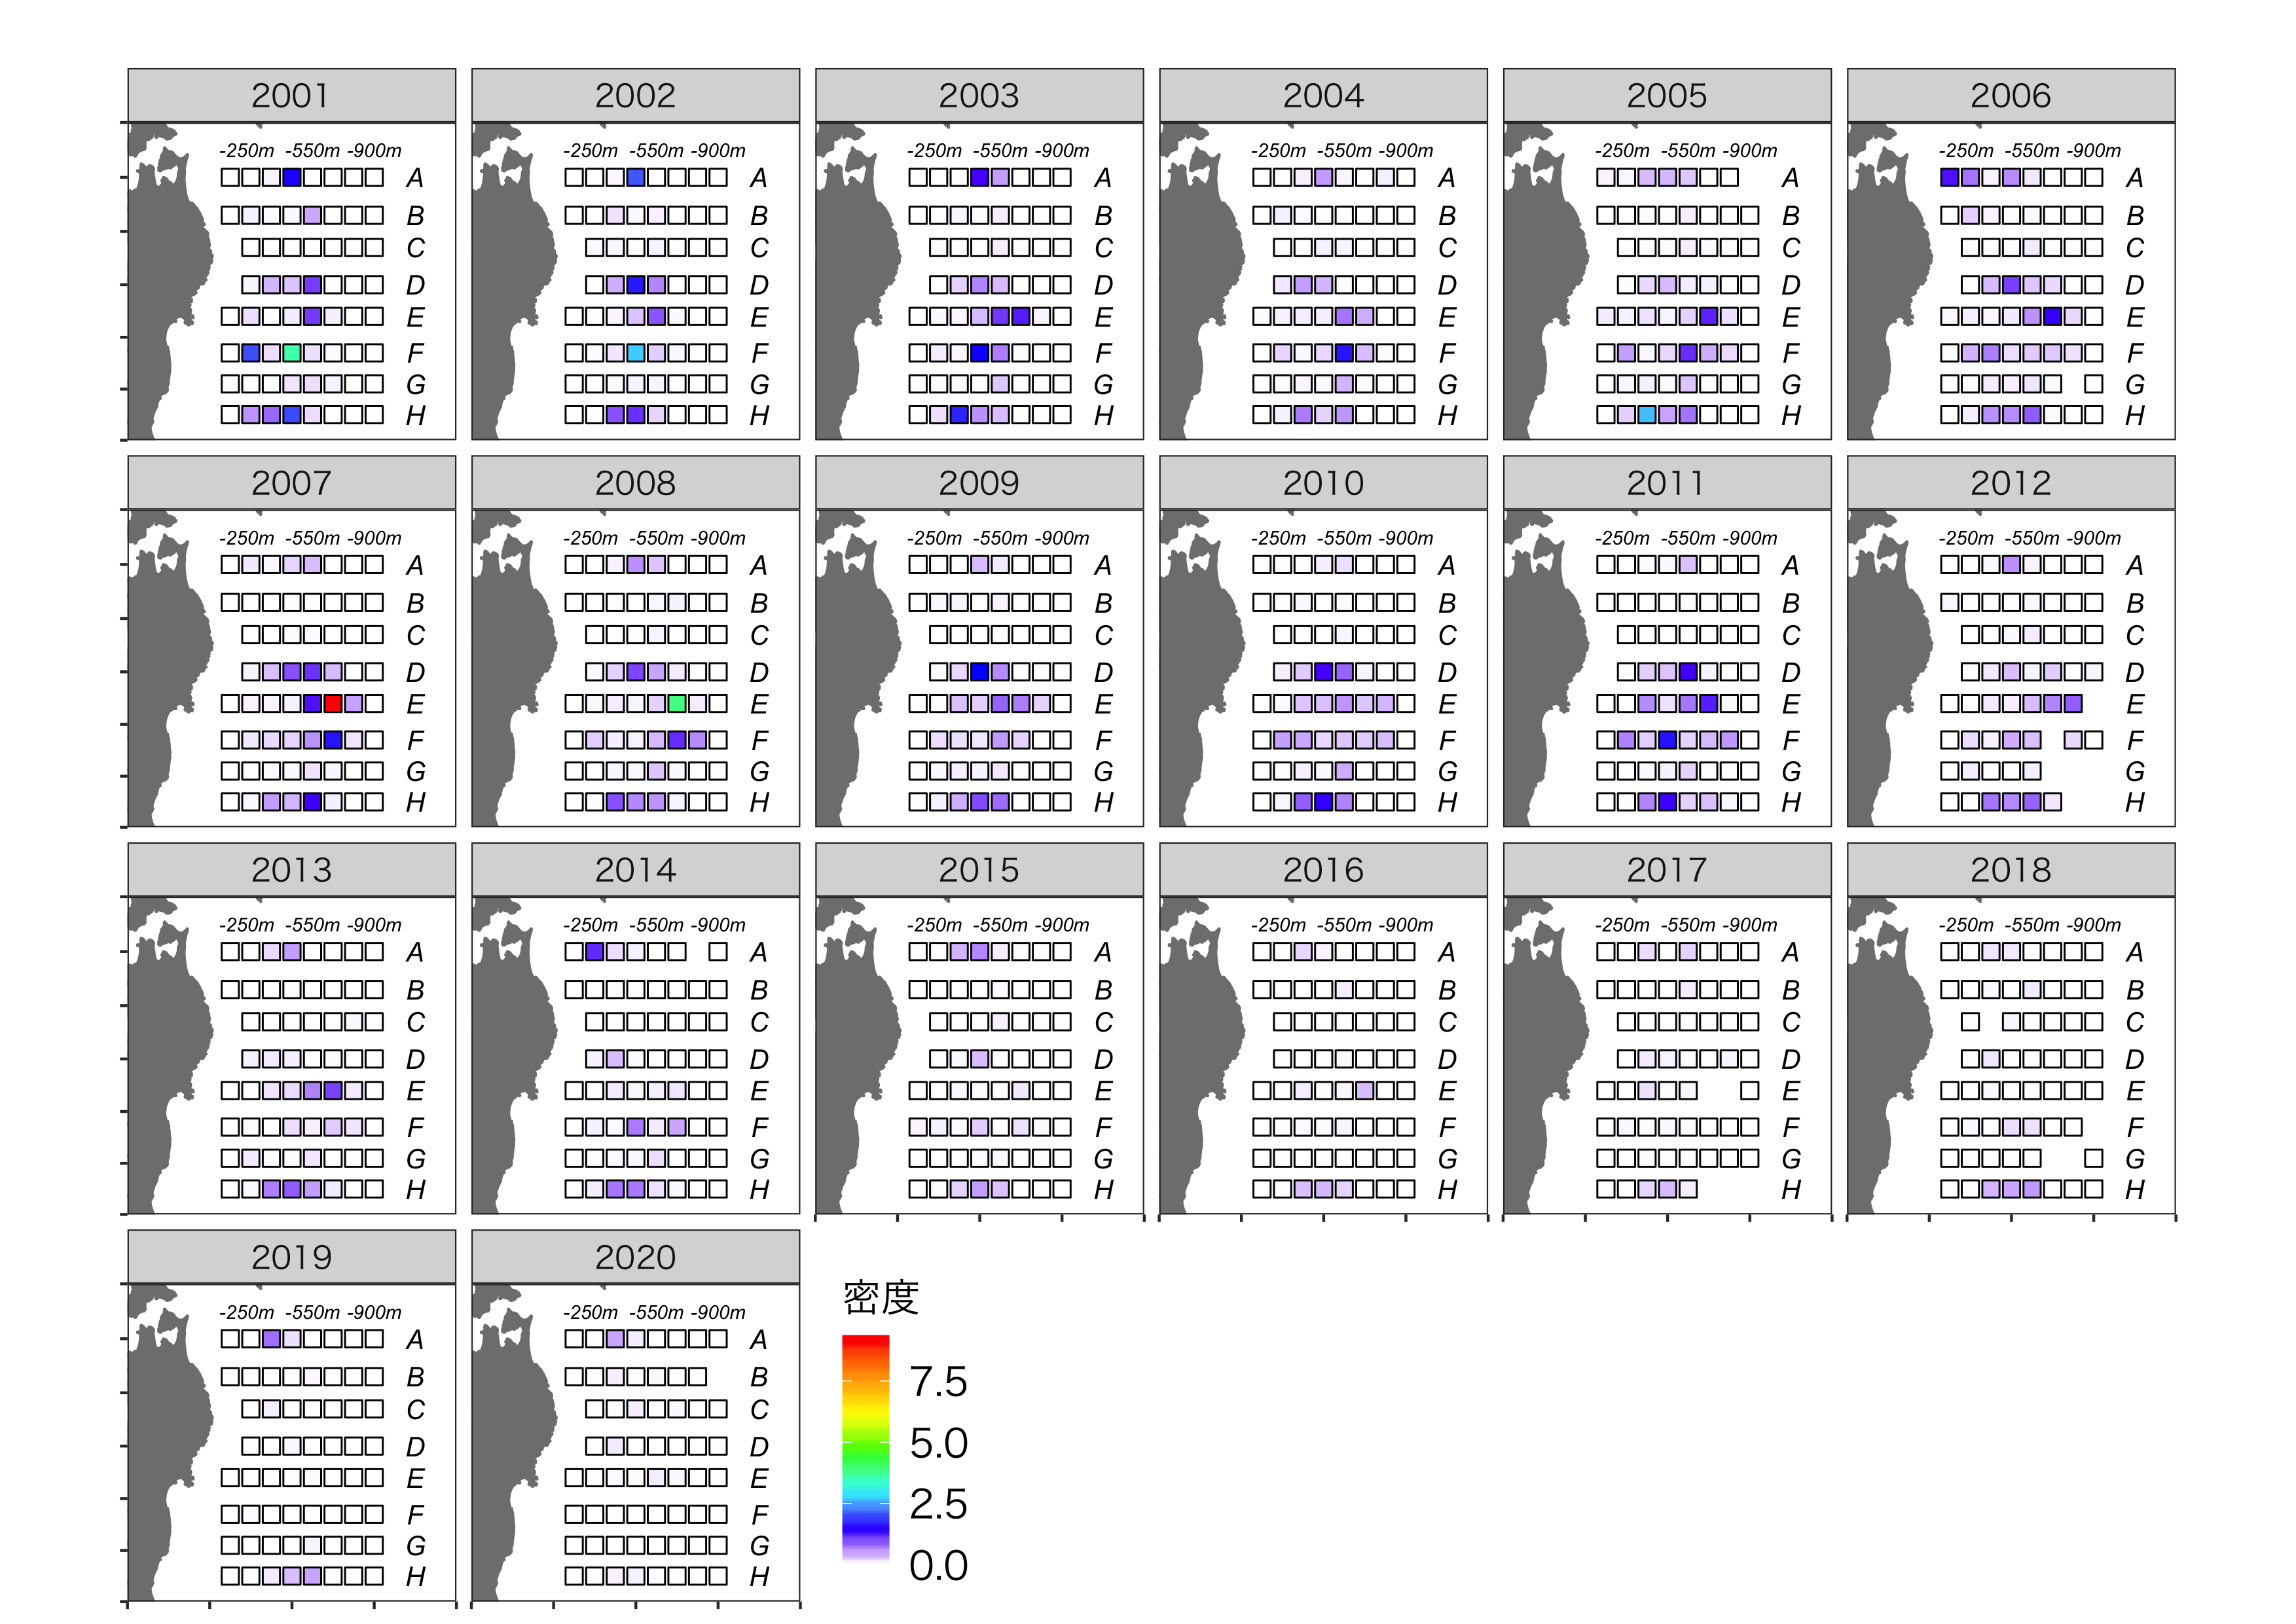
\includegraphics[width = 14cm]{アカガレイdens.png}
  \caption{アカガレイの分布密度(千尾/km2)の経年変化}
\end{figure}

\begin{figure}[h]
  \centering
  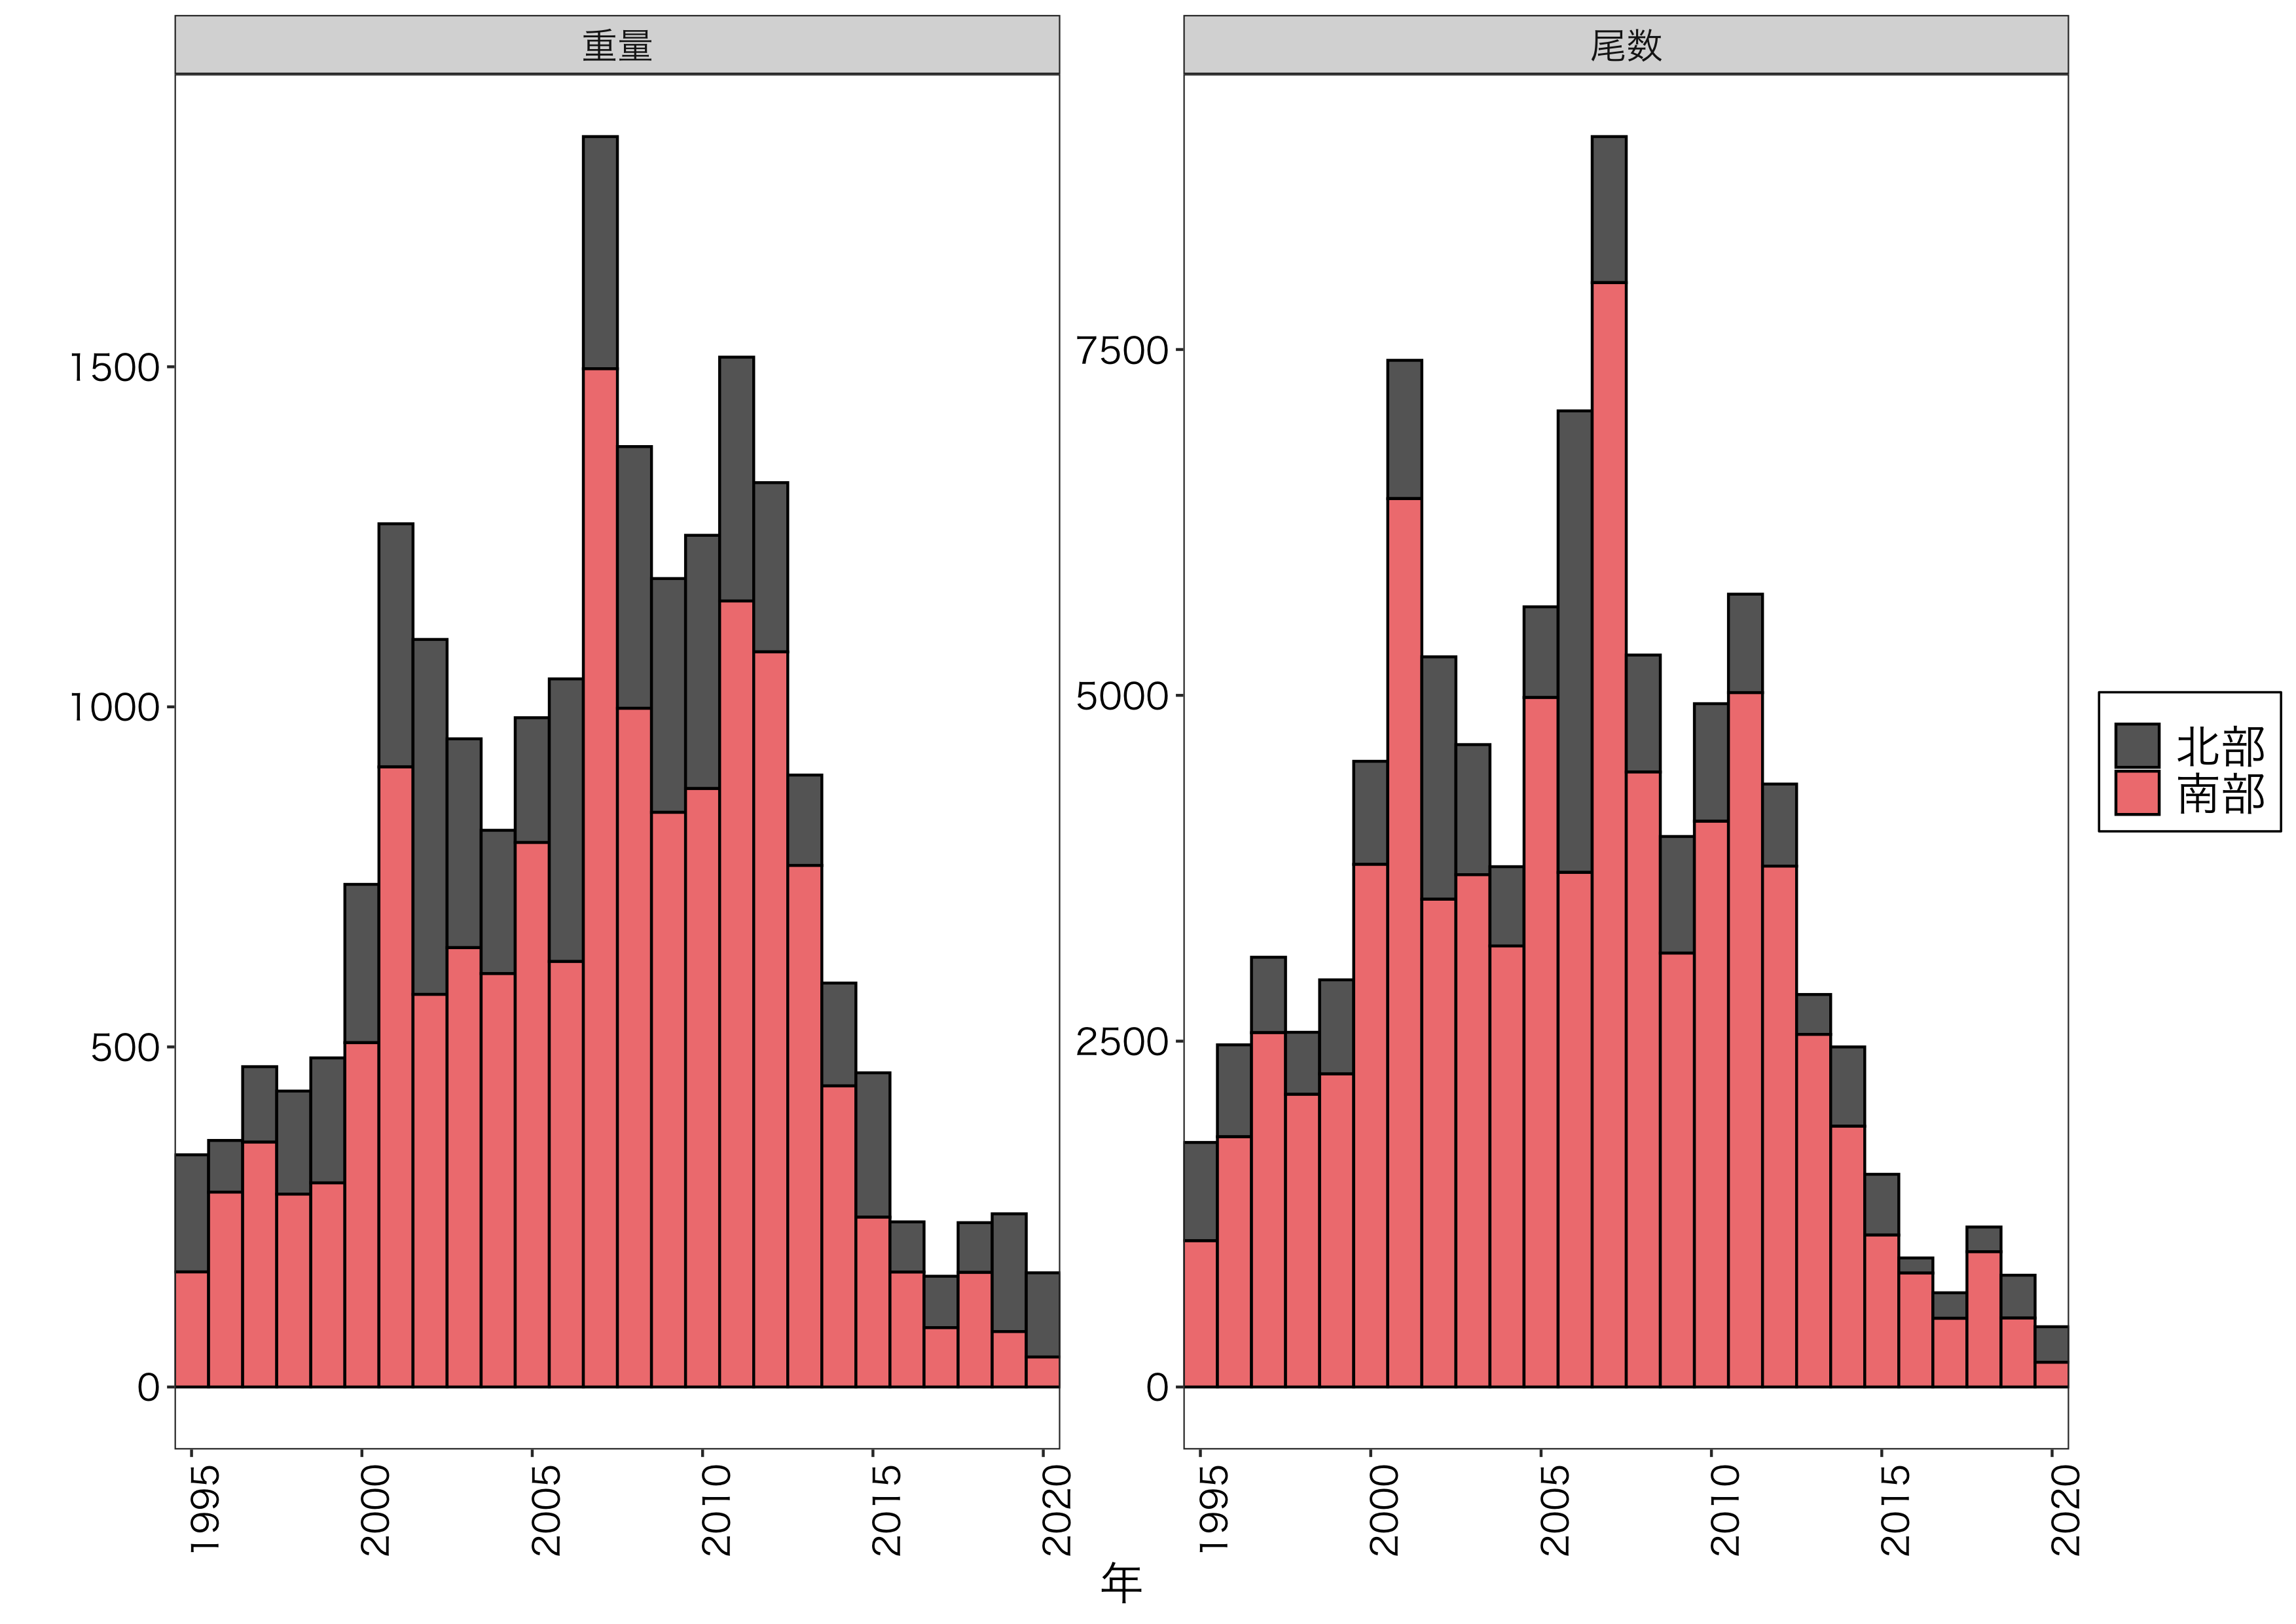
\includegraphics[width = 14cm]{アカガレイtrend.png}
  \caption{アカガレイの現存量(右; 単位は千トンと現存尾数(左; 単位は百万尾))の経年変化}
\end{figure}

\begin{figure}[h]
  \centering
  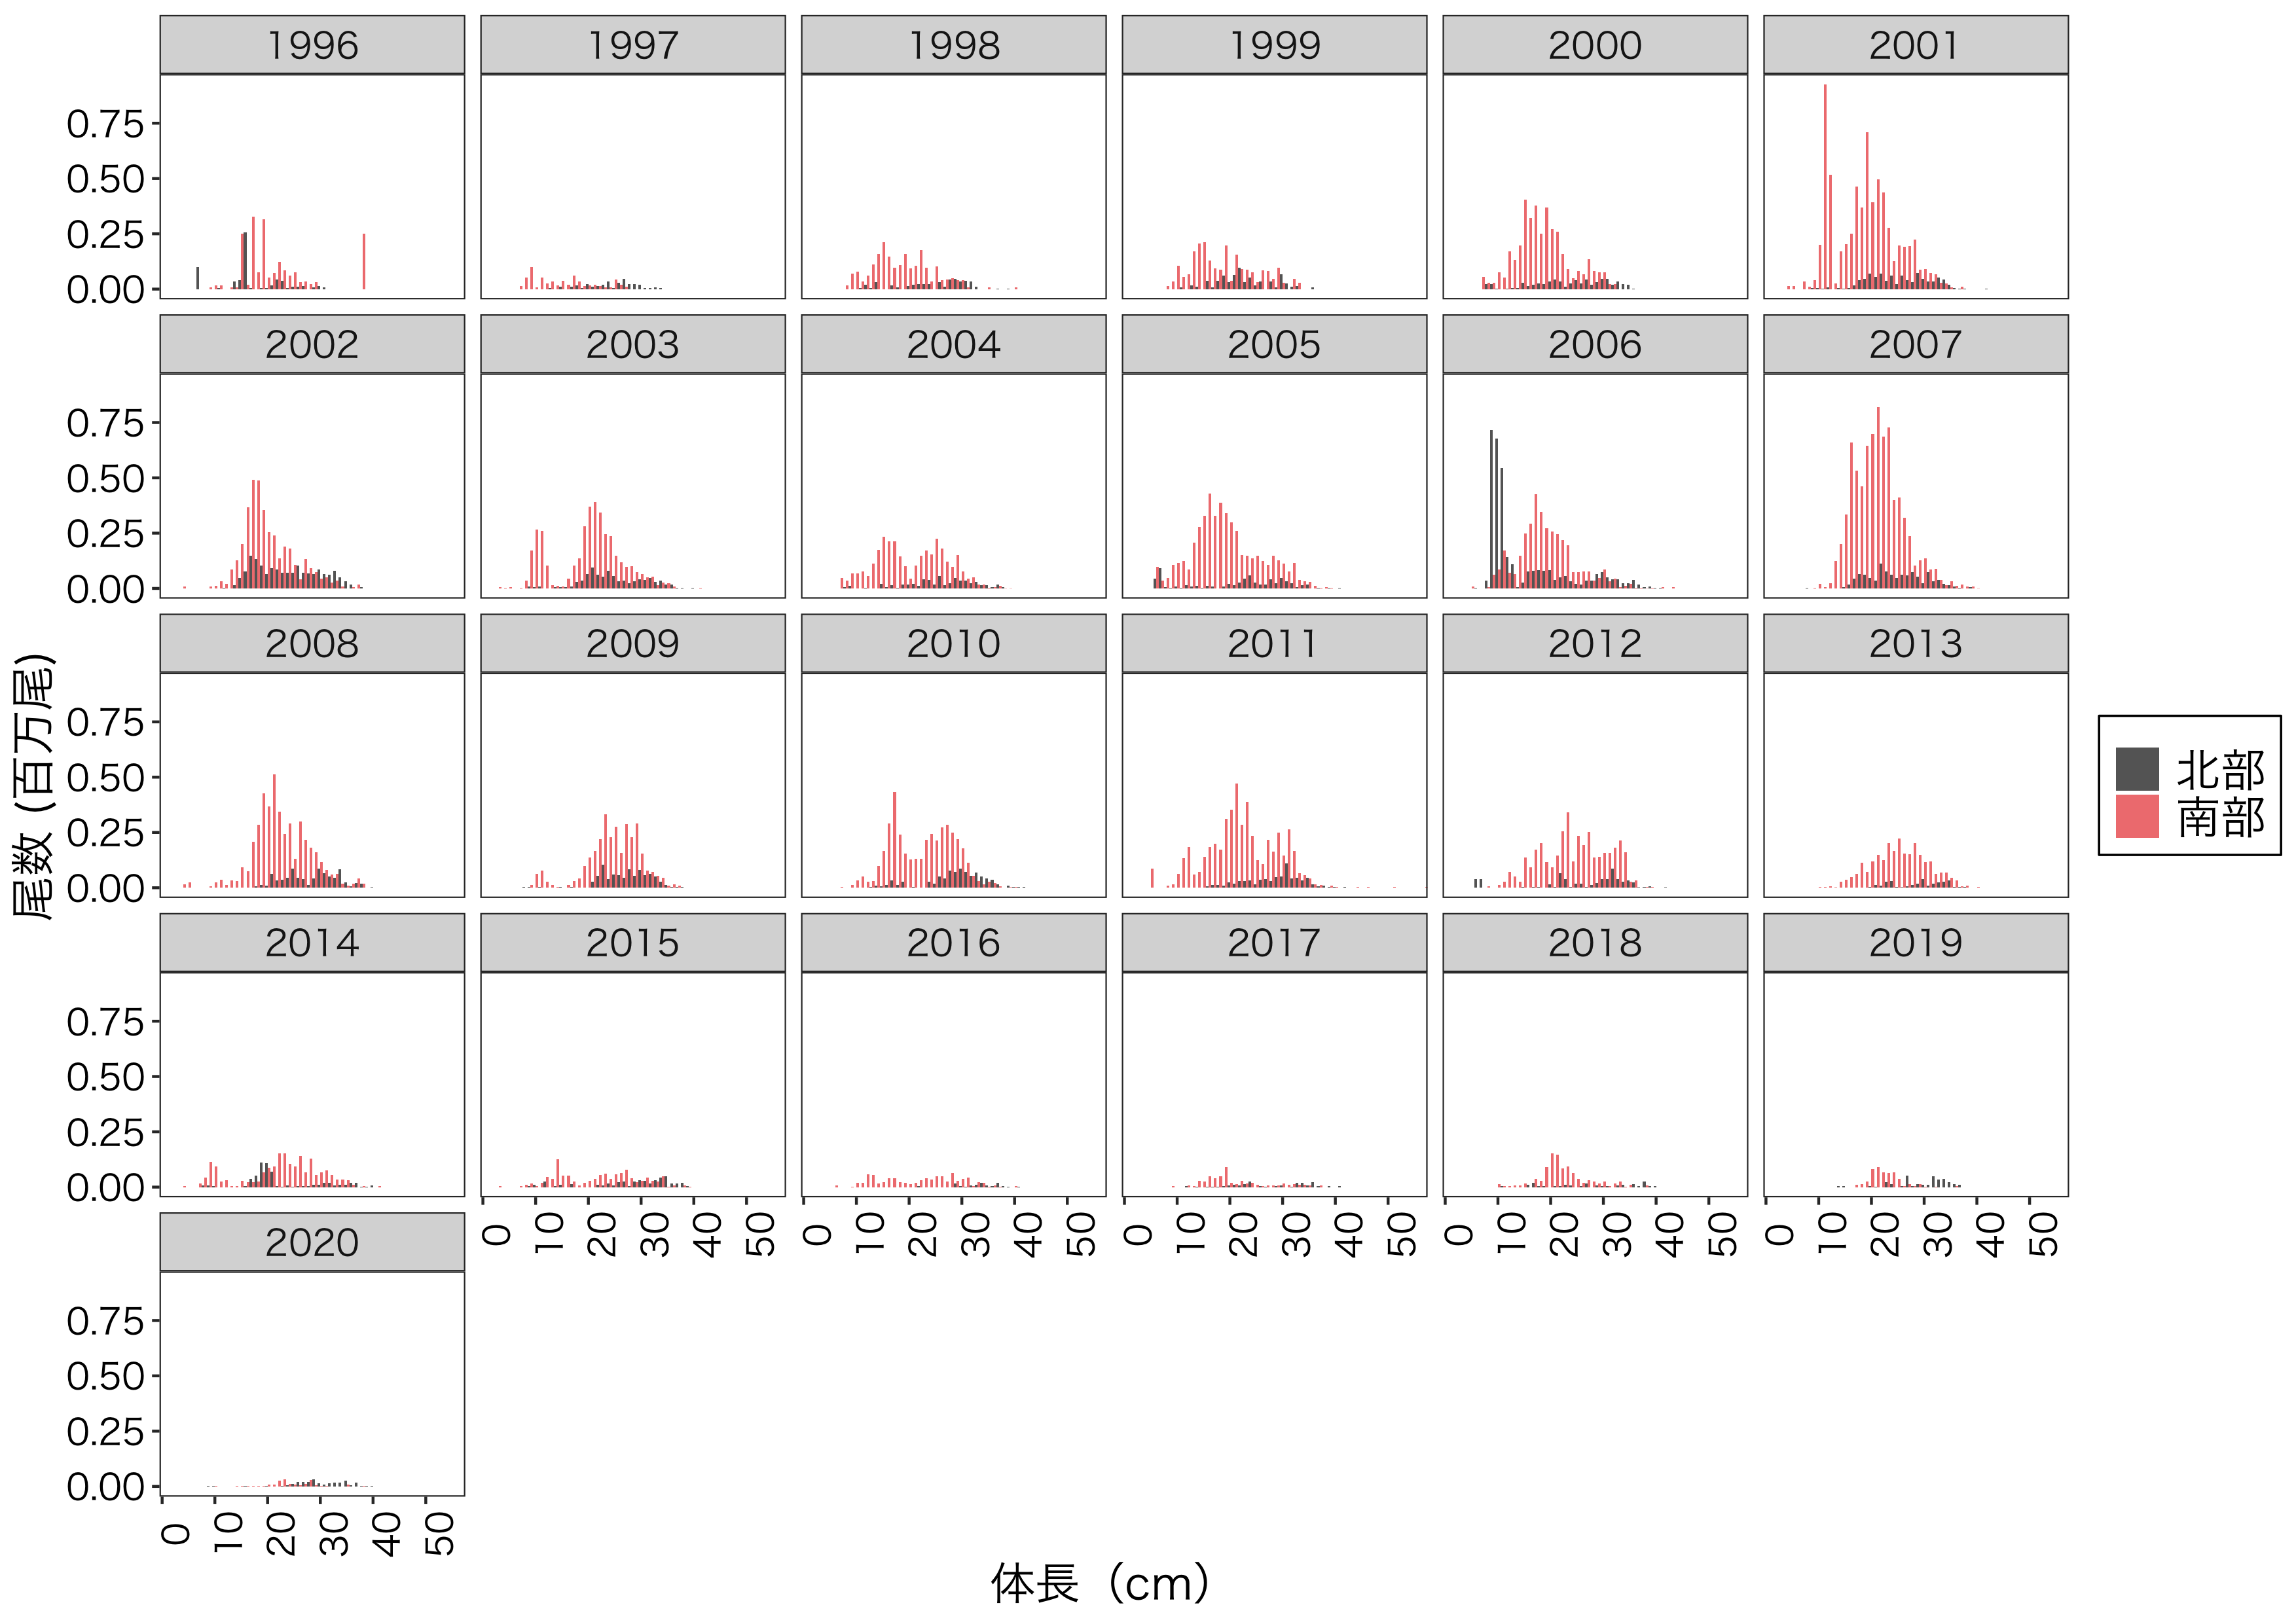
\includegraphics[width = 14cm]{アカガレイlength.png}
  \caption{アカガレイの体長組成の経年変化}
\end{figure}

\begin{figure}[h]
  \centering
  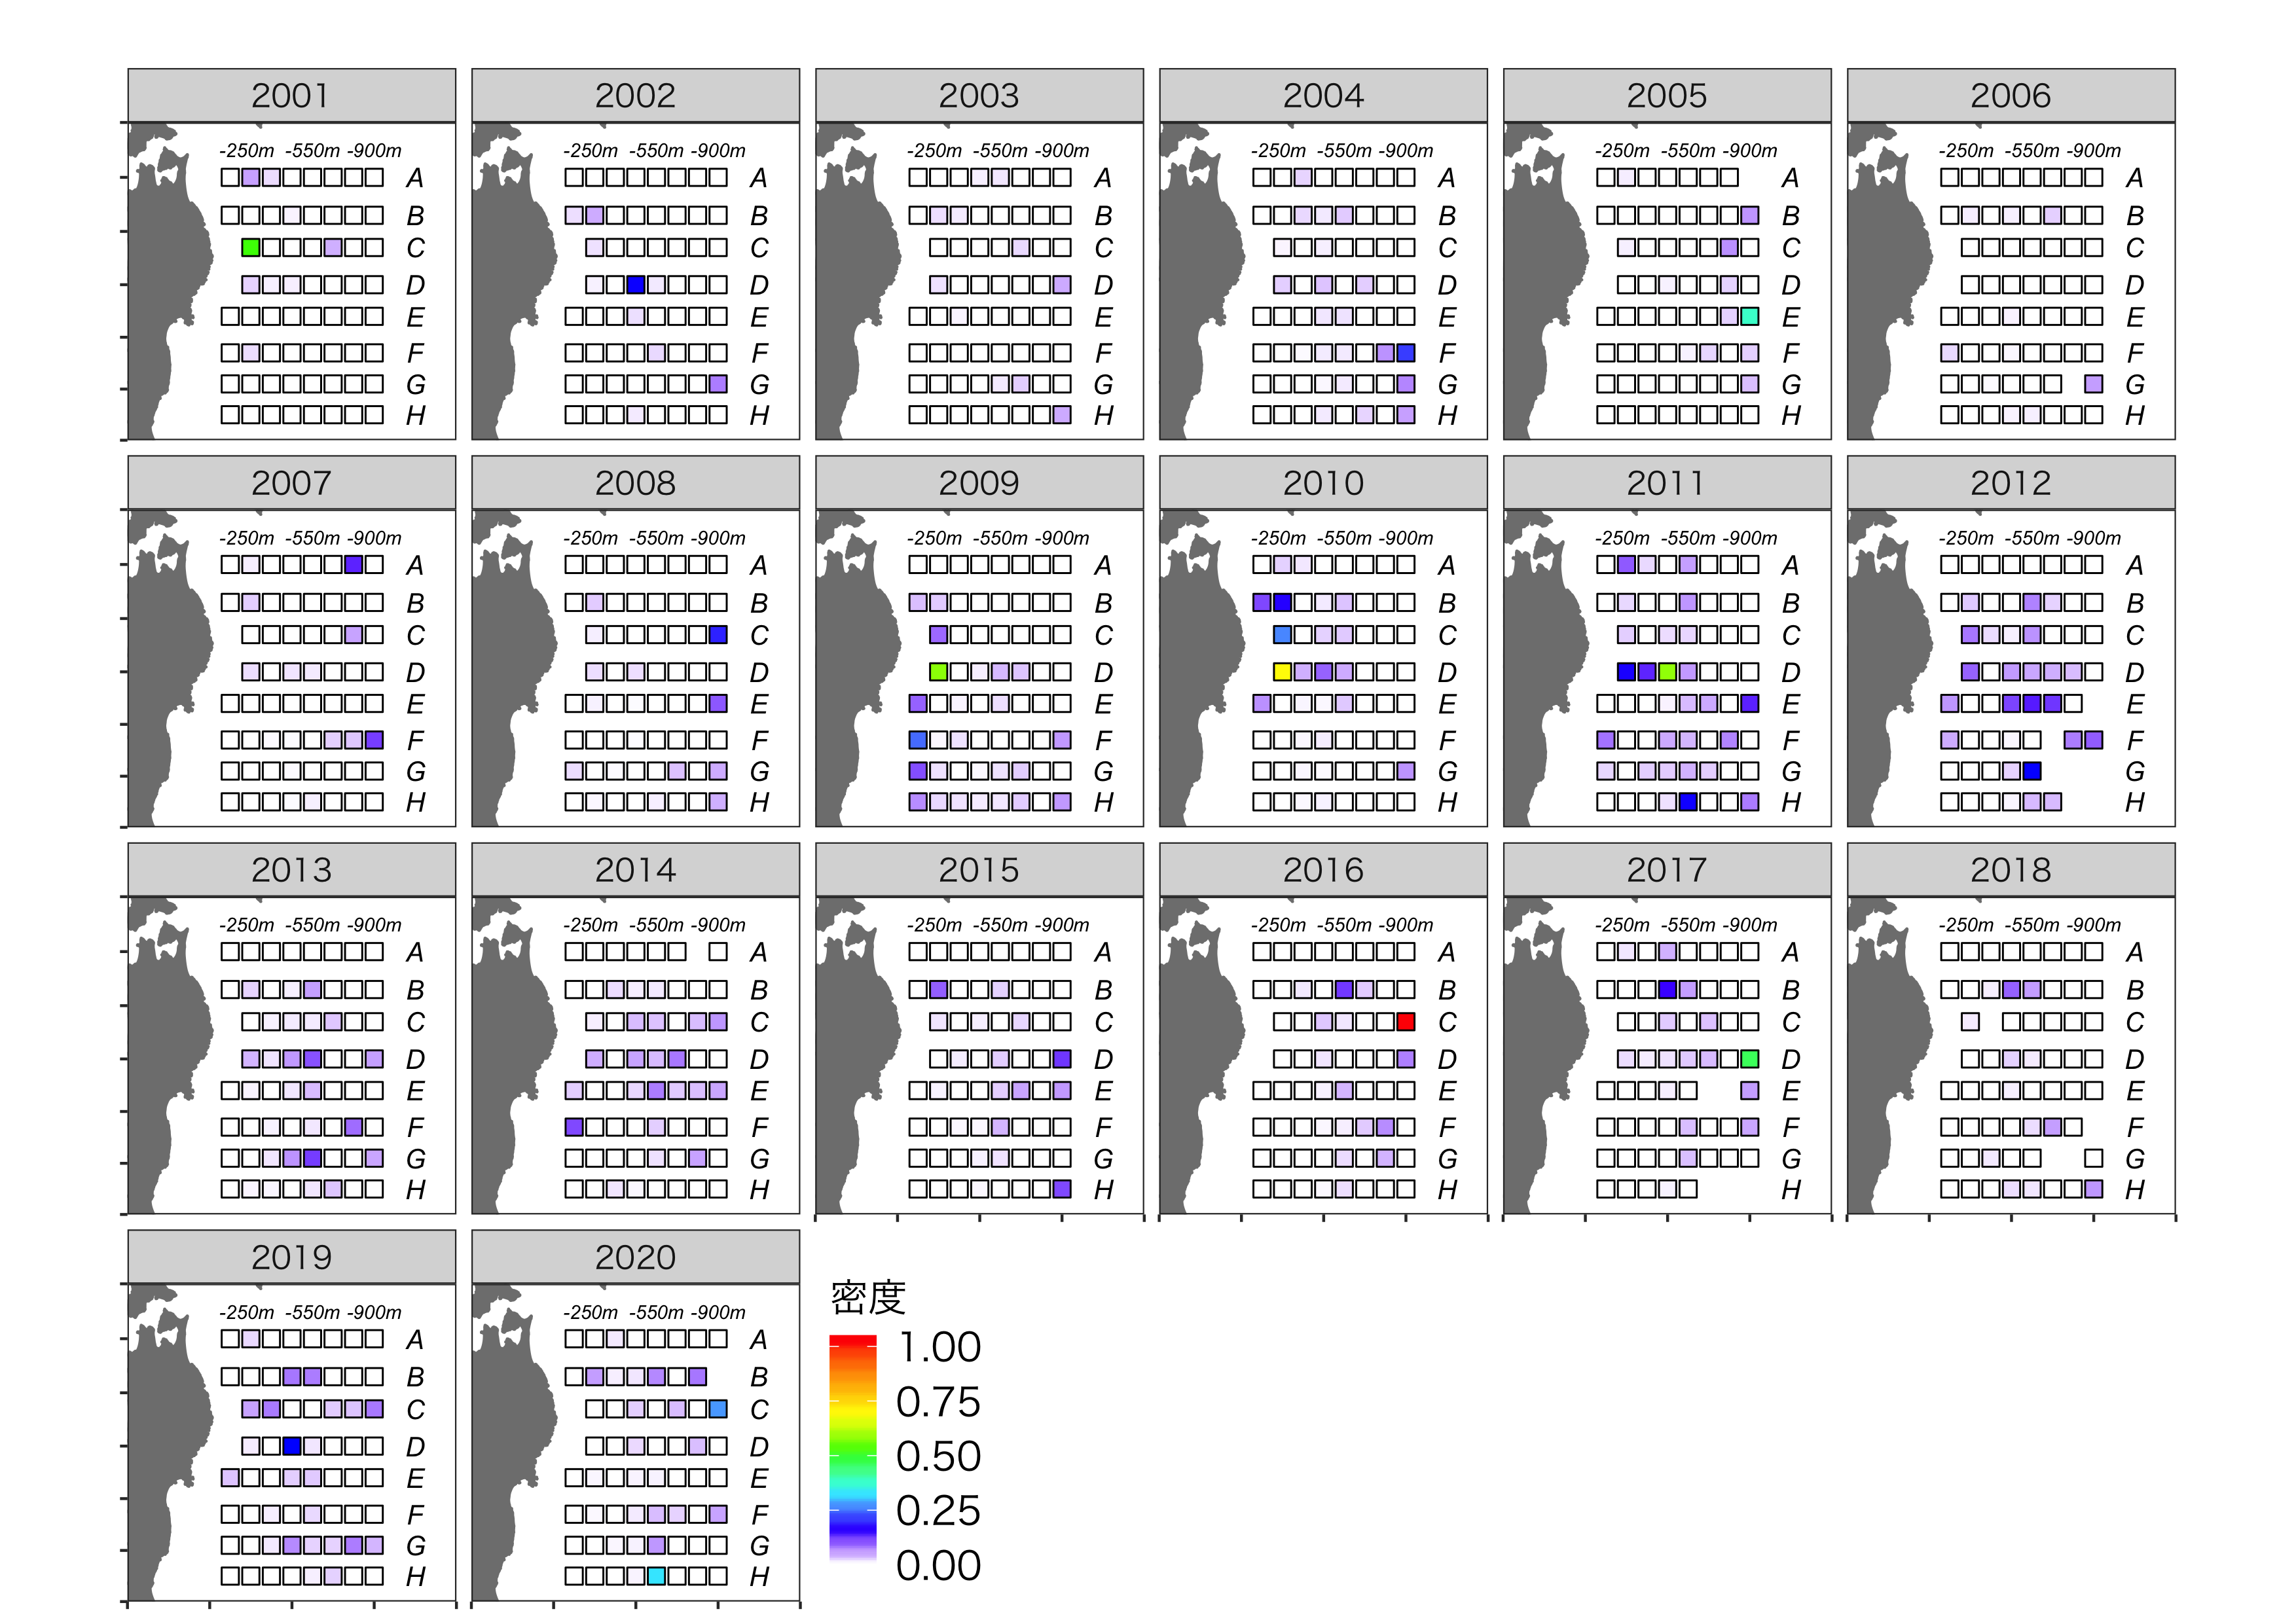
\includegraphics[width = 14cm]{サメガレイdens.png}
  \caption{サメガレイの分布密度(千尾/km2)の経年変化}
\end{figure}

\begin{figure}[h]
  \centering
  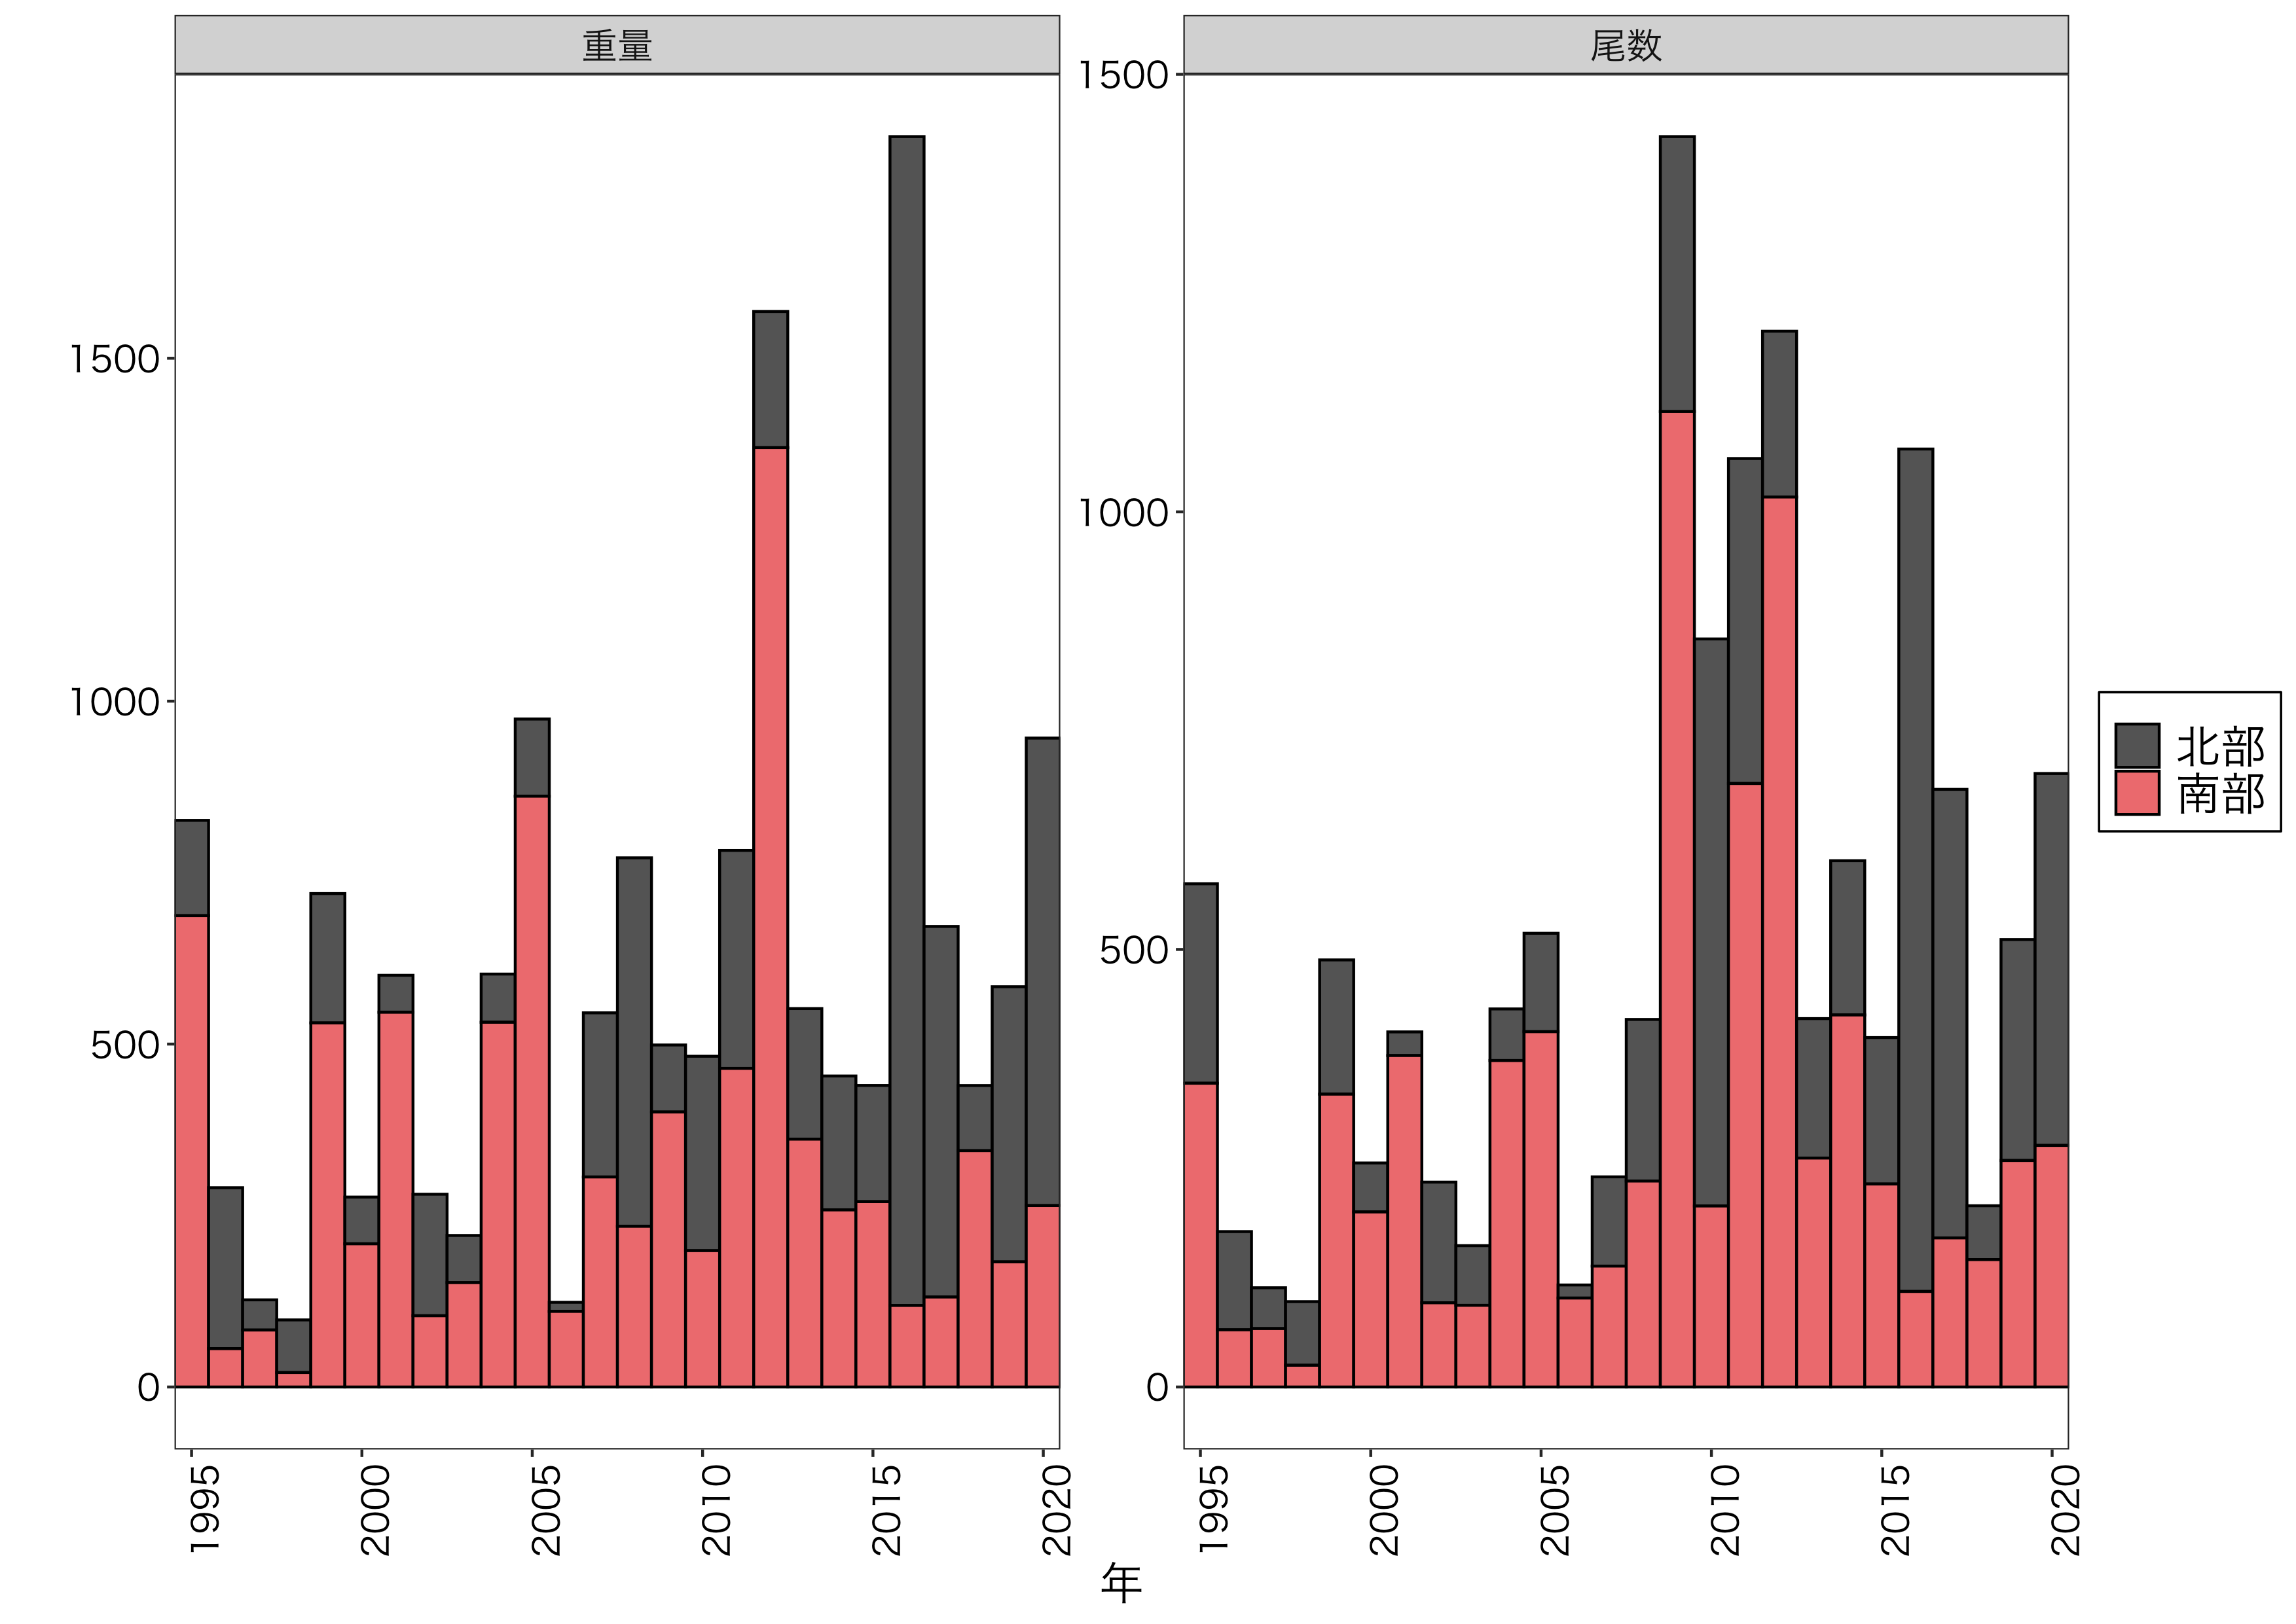
\includegraphics[width = 14cm]{サメガレイtrend.png}
  \caption{サメガレイの現存量(右; 単位は千トン)と現存尾数(左; 単位は百万尾)の経年変化}
\end{figure}

\begin{figure}[h]
  \centering
  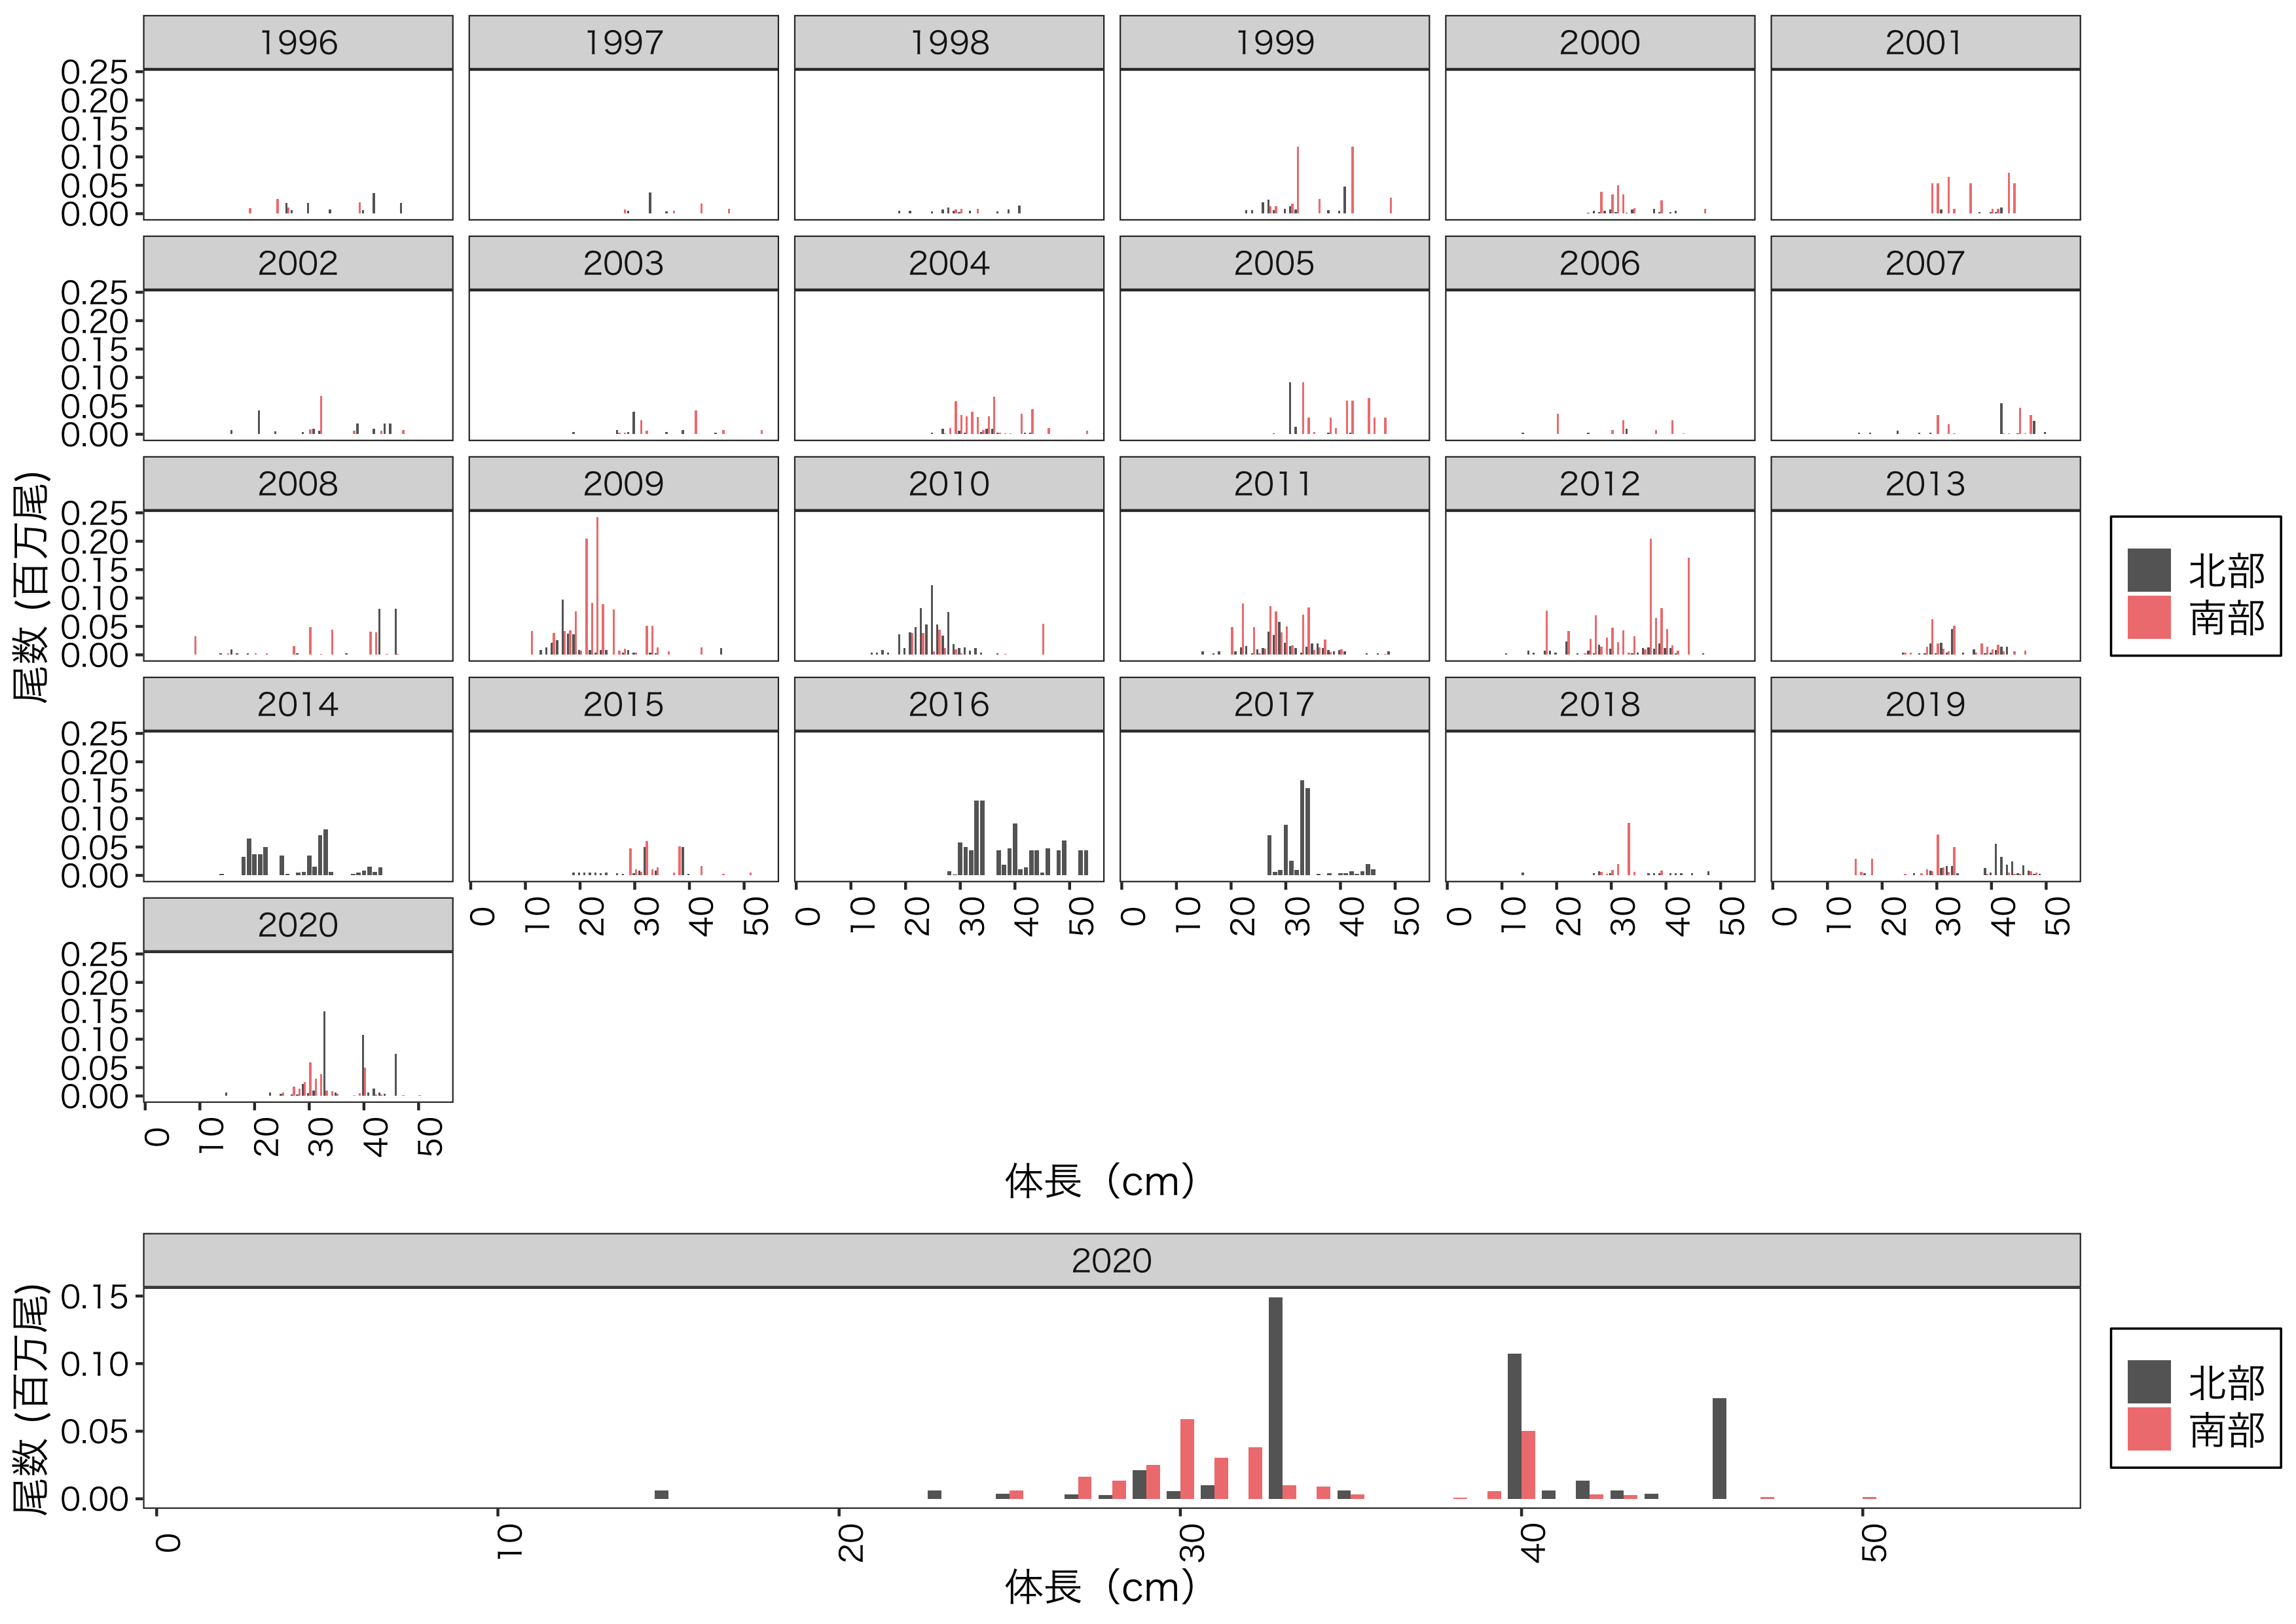
\includegraphics[width = 14cm]{サメガレイlength.png}
  \caption{サメガレイの体長組成の経年変化}
\end{figure}

\begin{figure}[h]
  \centering
  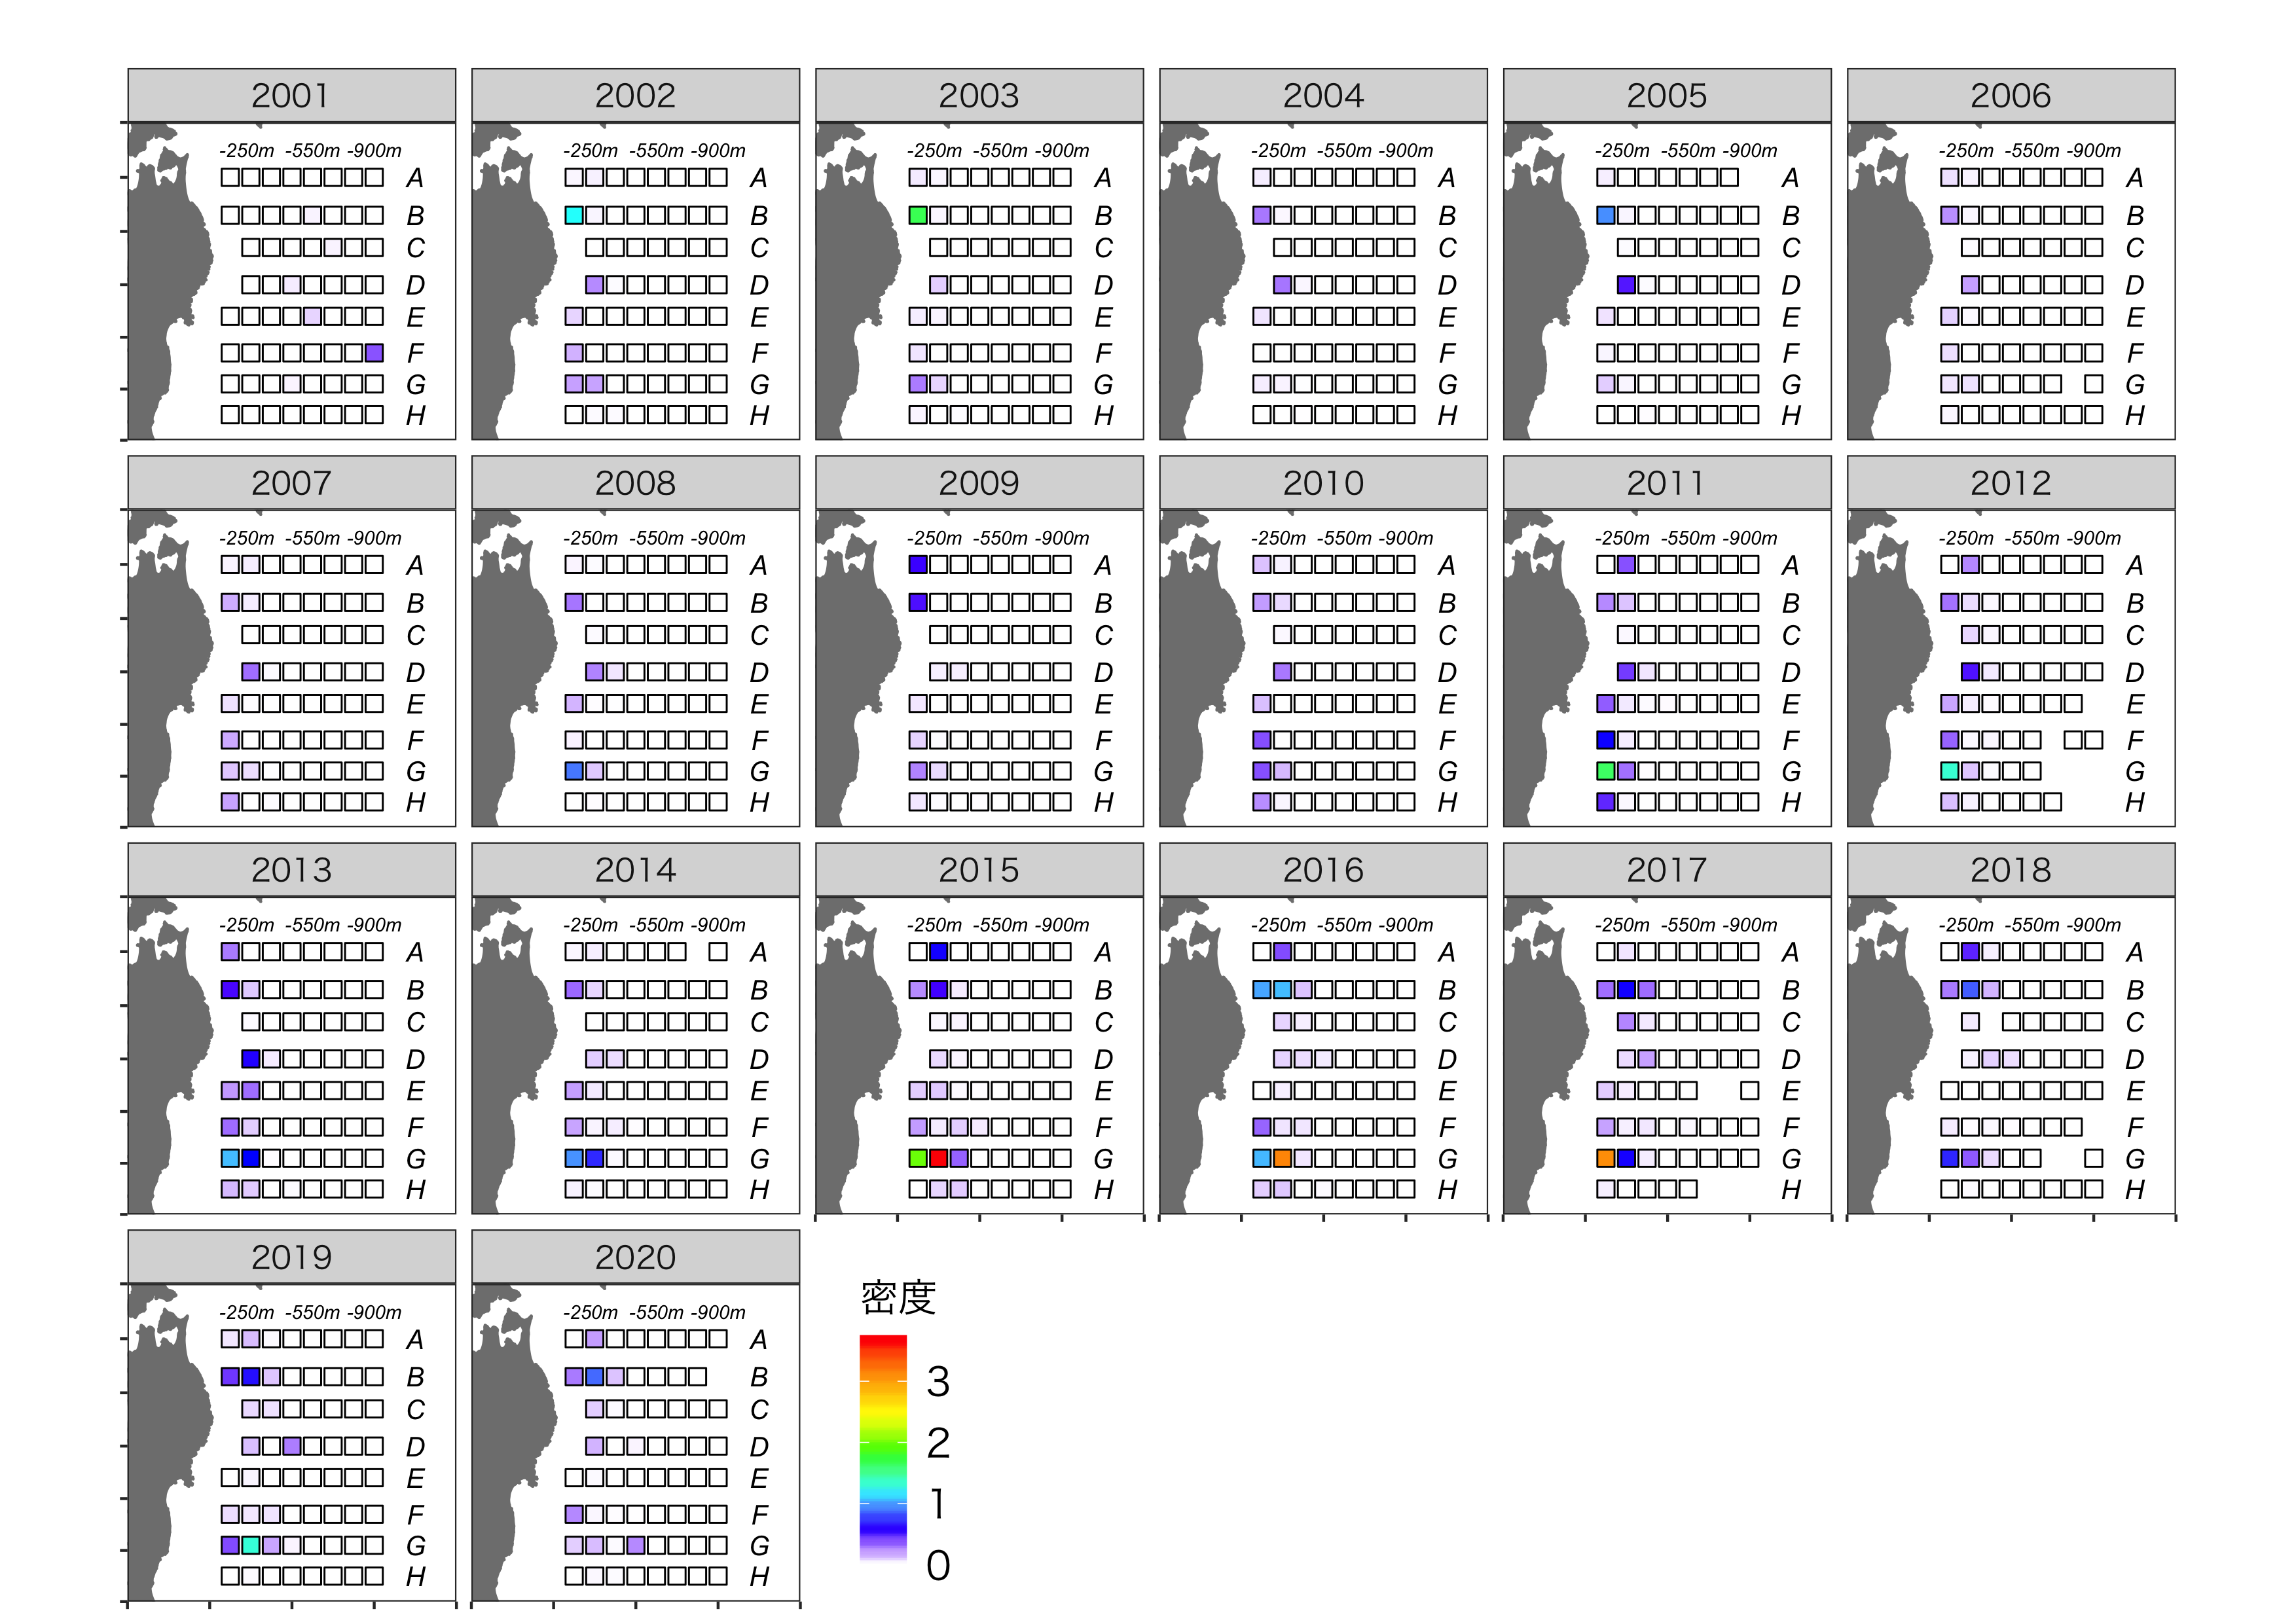
\includegraphics[width = 14cm]{ババガレイdens.png}
  \caption{ババガレイの分布密度(千尾/km2)の経年変化}
\end{figure}

\begin{figure}[h]
  \centering
  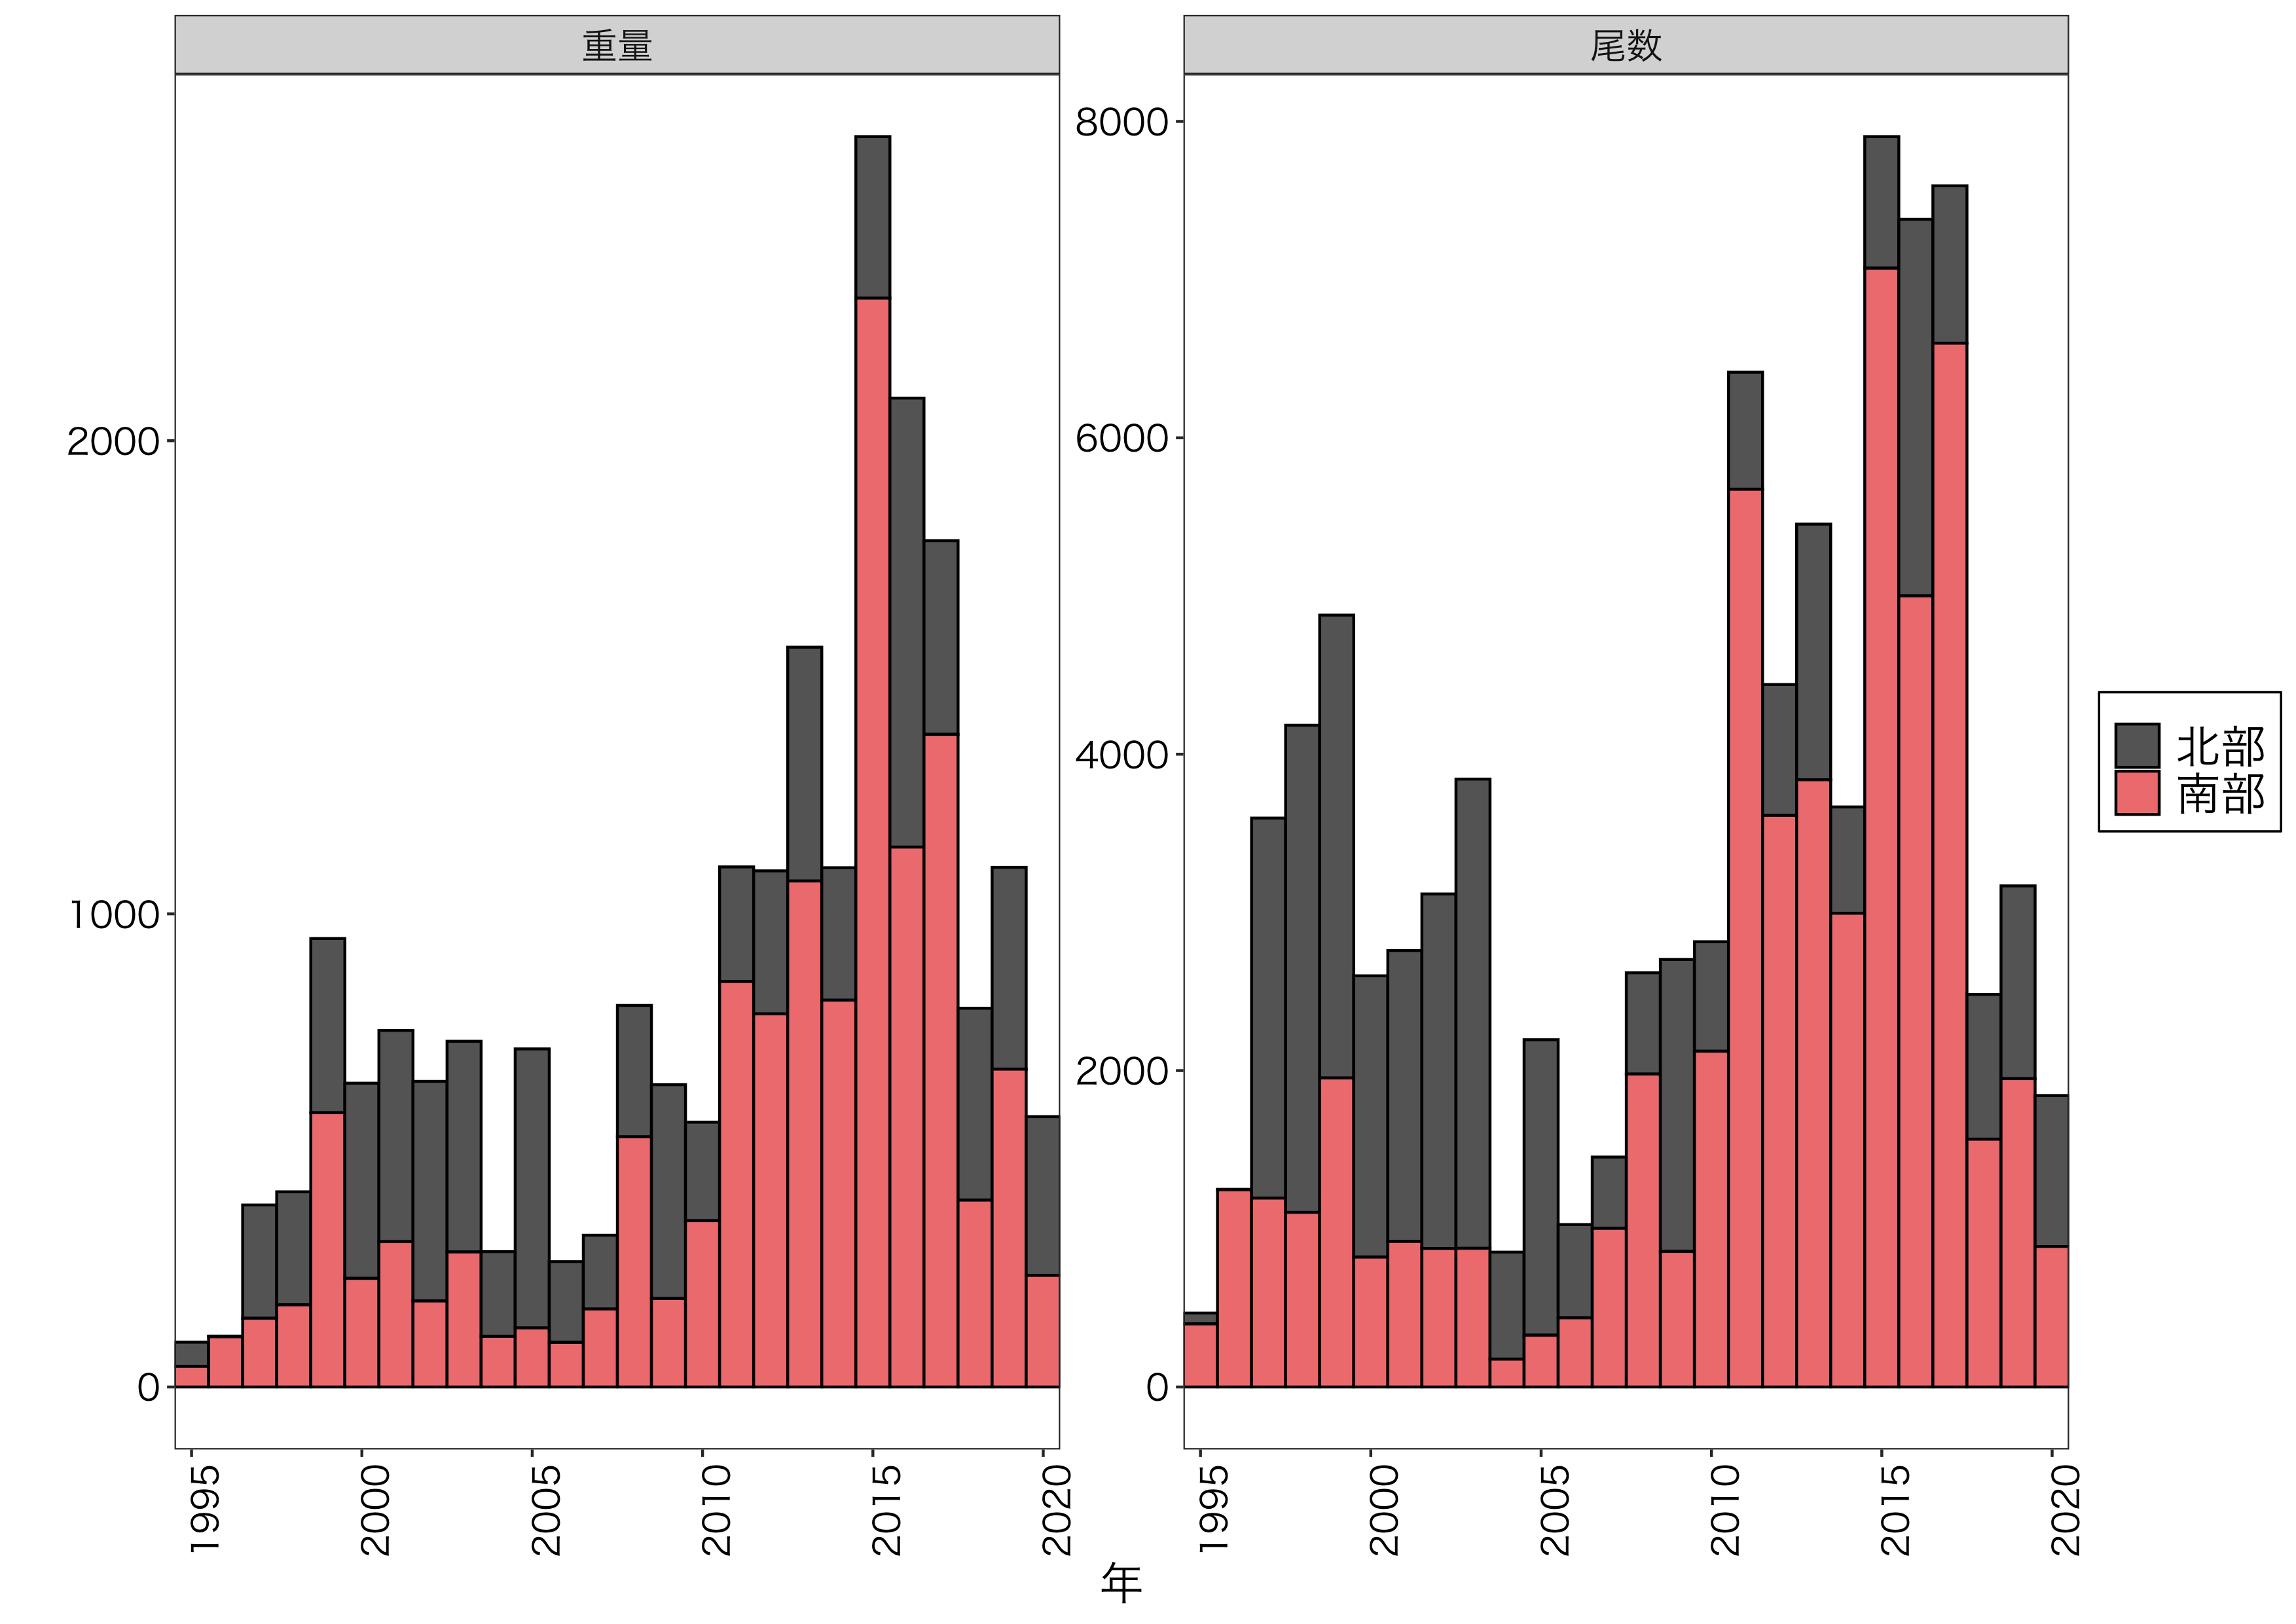
\includegraphics[width = 14cm]{ババガレイtrend.png}
  \caption{ババガレイの現存量(右; 単位は千トン)と現存尾数(左; 単位は百万尾)の経年変化}
\end{figure}

\begin{figure}[h]
  \centering
  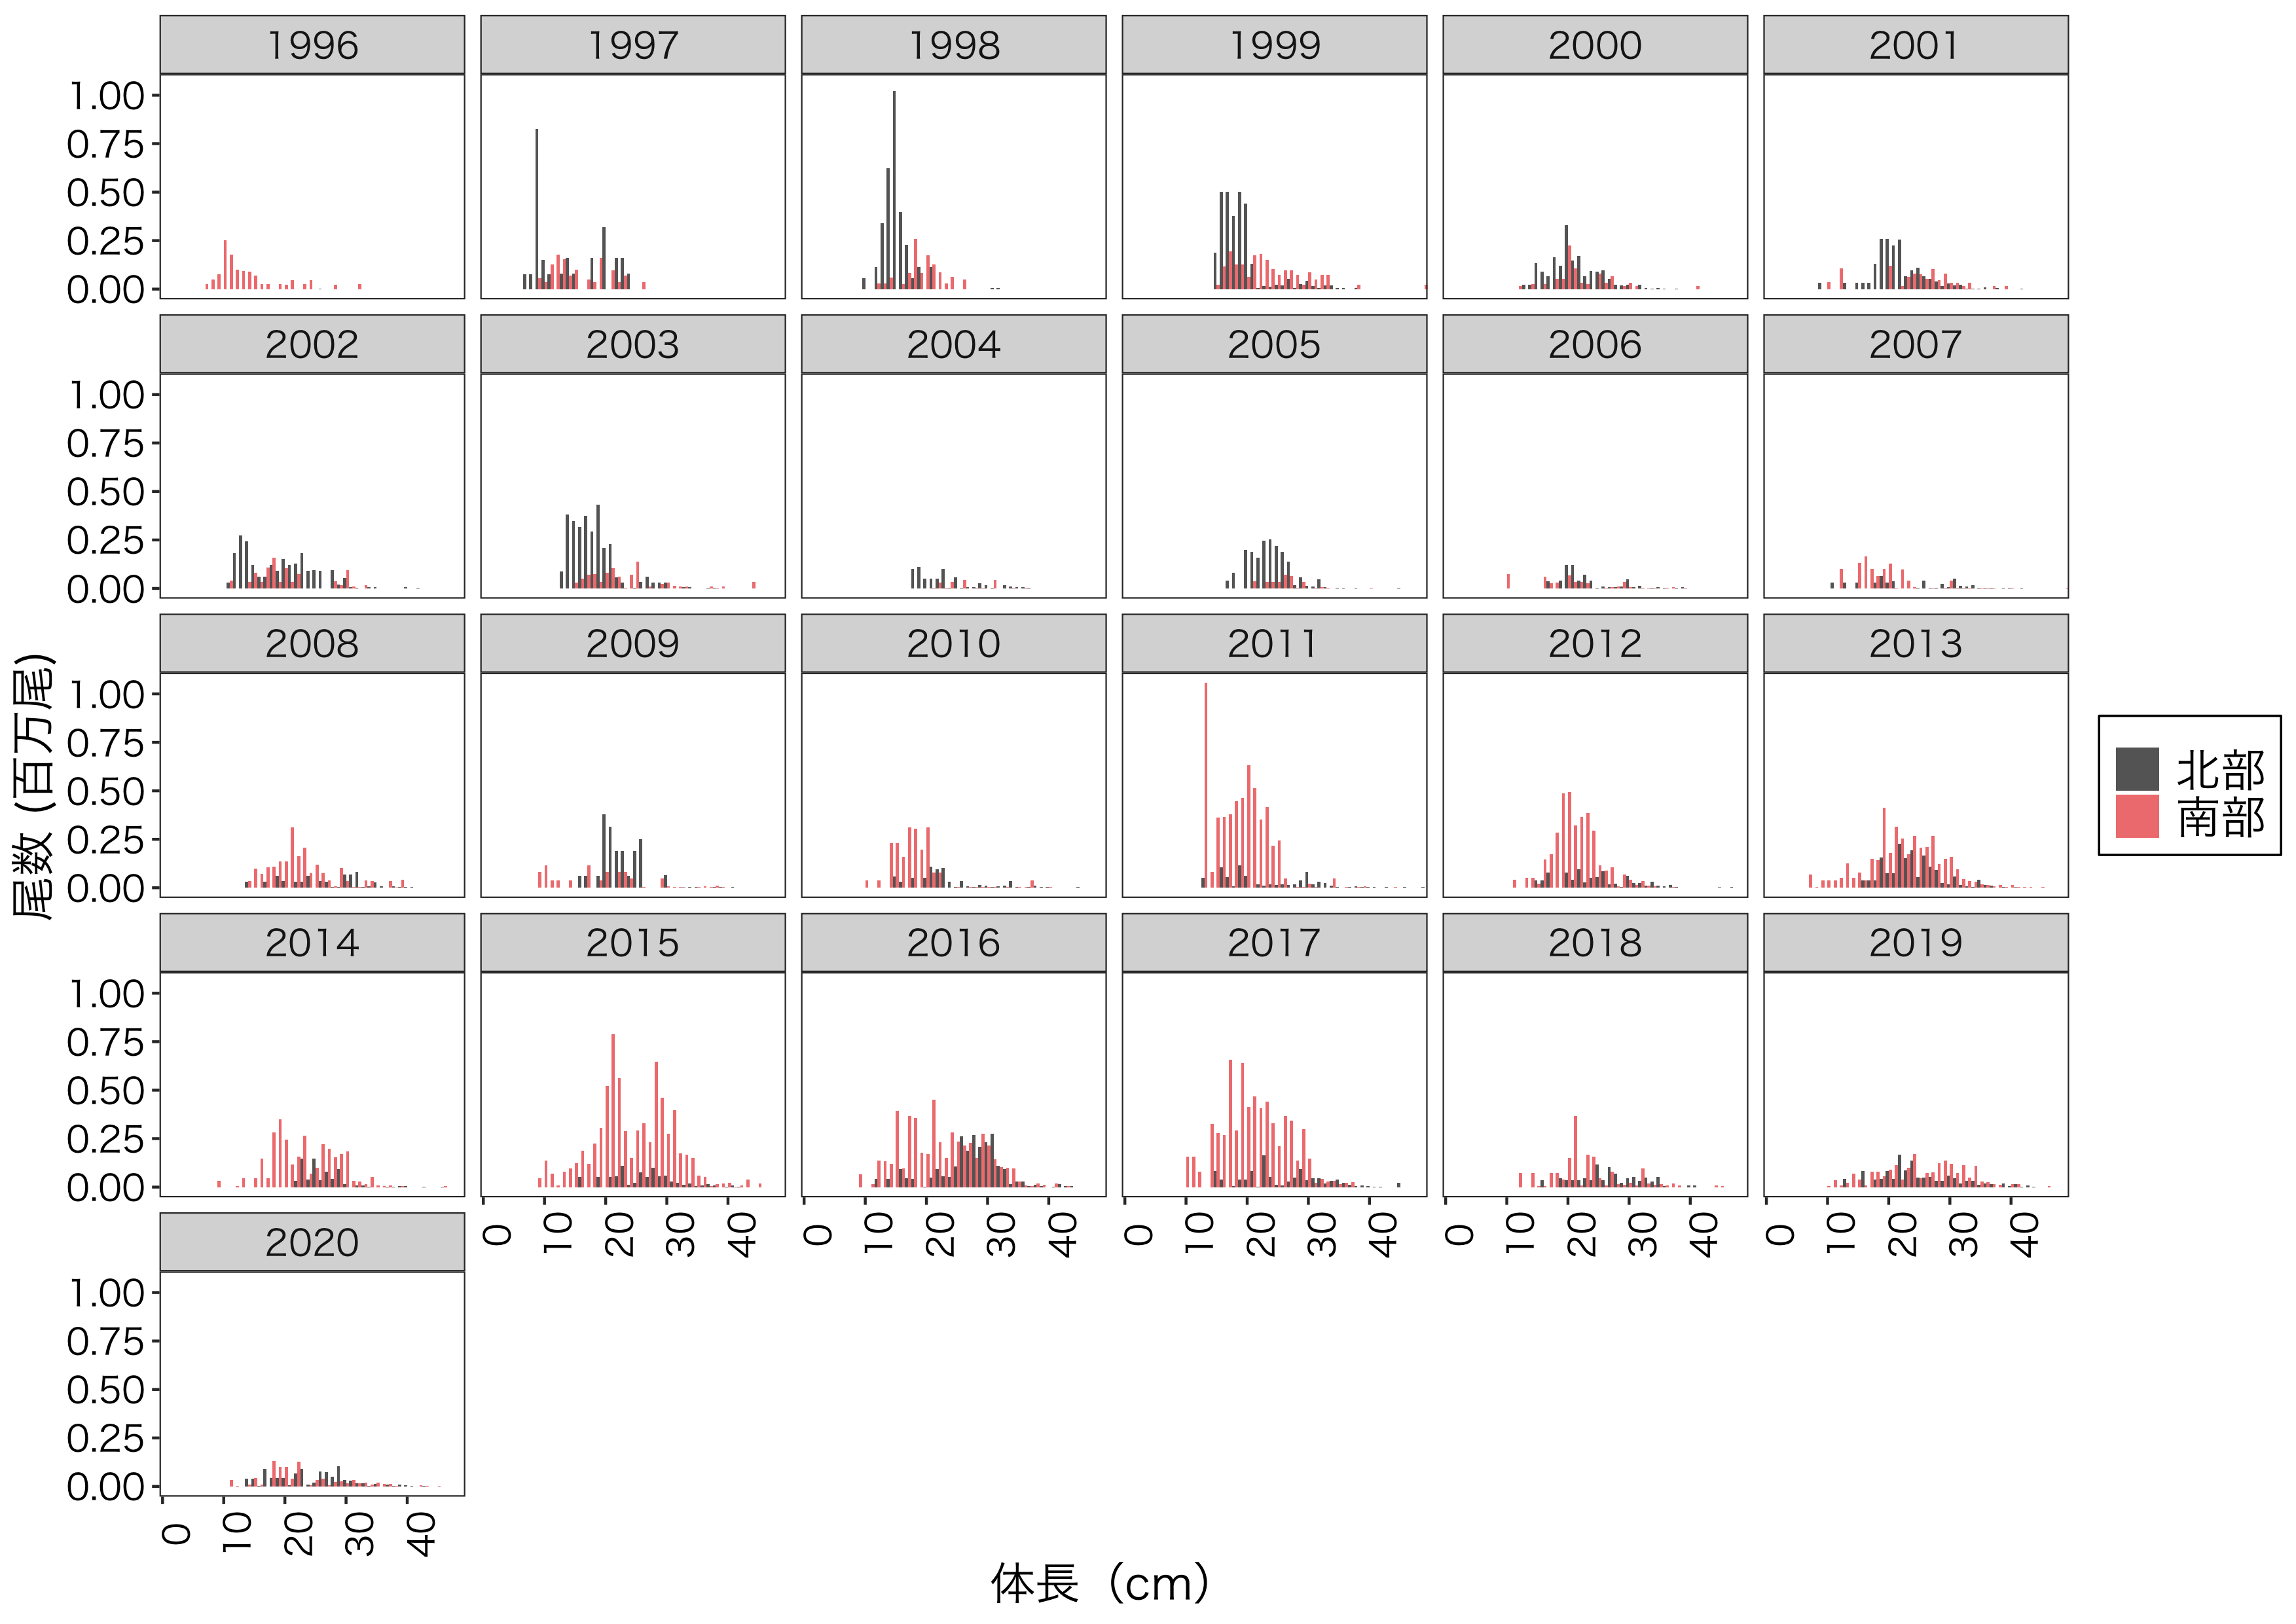
\includegraphics[width = 14cm]{ババガレイlength.png}
  \caption{ババガレイの体長組成の経年変化}
\end{figure}

\end{linenumbers}
\end{document}